%% TeX mode: XeLaTeX + bibTeX + XeLaTeX + XeLaTeX

%% Thesis Template of Guangzhou University
%% for using GZHUthesis package with LaTeX2e Created by Viming Wei
%% <weiviming@gmail.com> 2019-5.

\PassOptionsToPackage{quiet}{fontspec} % 消除字体警告
\expandafter\def\csname CTEX@spaceChar\endcsname{\hspace{1em}}
\documentclass[openany, notypeinfo]{style/GZHUthesis}

% 可选参数:
% openany    新一章从奇数页或偶数页开始都可以
% notypeinfo 取消扉页的LaTeX版本信息
%
% 下面三个选一个:
% 使用 dvipdfm  生成最终的 PDF 文档 (缺省设置)
% 使用 dvips    生成最终的 PS 文档
% 使用 pdfLaTeX 生成最终的 PDF 文档

%盲审模式,正常模式请注释掉
%\blindtrue
\blindfalse

%默认博士论文, 如需要硕士论文, 注释掉下行
\phdtrue
%\phdfalse

%字体设置
\setsansfont{Arial}

%\citeyearn{XXXX} 自动在\citeyear后面加上“年”
\hypersetup{hidelinks} %取消链接的颜色

%% 为了方便输入特殊符号, 添加如下新命令:
\medmuskip=2mu        %水平间距调整: 二元运算符 "+, -, <"
\thickmuskip=3mu      %水平间距调整: 关系符号调整 "="
% \abovedisplayskip=0pt
% \belowdisplayskip=0pt
% \abovedisplayshortskip=0pt
% \belowdisplayshortskip=0pt


\graphicspath{{chapter/}{figures/}}  % 设置图形文件的搜索路径
\ctexset{section={format+={\flushleft}}}  % 小节标题靠左对齐

% 添加新文件时, 需要在此处加入文件名, 方便控制编译结果
\ifblind
\includeonly{  %% 选择盲审时要编译的章节
  chapter/abstract,
  chapter/chapter1,
  chapter/chapter2,
  chapter/chapter3,
  chapter/chapter4,
  chapter/chapter5,
  chapter/conclusion,
}
\else
\includeonly{  %% 选择要编译的章节, 注释掉的章节不会编译, 平时可注释掉某些章节来提升整体编译速度
  chapter/abstract,
  chapter/chapter1,
  chapter/chapter2,
  chapter/chapter3,
  chapter/chapter4,
  chapter/chapter5,
  chapter/conclusion,
  chapter/Abbreviation,
  chapter/publications,
  chapter/projects,
  chapter/thanks
}
\fi


% 自定义命令
% !TEX root = ../main.tex
% 常用符号与自定义命令
\def\ZZ{{\mathbb Z}}
\def\NN{{\mathbb N}}
\def\RR{{\mathbb R}}
\def\CC{{\mathbb C}}
\def\QQ{{\mathbb Q}}
\def\EE{{\mathbb E}}
\def\FF{{\mathbb F}}
\def\Fp{\mathbb{F}_{p}}
\def\Fq{\mathbb{F}_{q}}
\def\Zp{\mathbb{Z}_{p}}
\def\Zq{\mathbb{Z}_{q}}
\def\Zk{\mathbb{Z}_{2^k}}
\def\Zl{\mathbb{Z}_{2^\ell}}

%\usepackage{pifont}
\newcommand{\cmark}{\ding{51}} % 打勾
\newcommand{\xmark}{\ding{55}} % 打叉

%% for algorithm
\floatname{algorithm}{算法}
\renewcommand{\algorithmicrequire}{\textbf{输入:}}
\renewcommand{\algorithmicensure}{\textbf{输出:}}

\newcommand{\upcite}[1]{\textsuperscript{\cite{#1}}} % 上标引用

% Protocol/Functionality
\tcbuselibrary{skins,breakable}
\newtcolorbox[auto counter,number within=chapter]{protocol}[2][]{%
  enhanced,
%  title        = {Protocol \thetcbcounter: {#2}},
  title        = {Protocol {#2}},
  attach boxed title to top left={xshift=+3mm,yshift*=-3mm},
  colback      = black!5,
  colframe     = black!35,
  fonttitle    = \bfseries,
  colbacktitle = black!15!white,
  arc          = 0mm,
  coltitle     = black,
  #1
}

\newtcolorbox[auto counter,number within=chapter]{functionality}[2][]{%
  enhanced,
%  title        = {Functionality \thetcbcounter: {#2}},
  title        = {Functionality {#2}},
  attach boxed title to top left={xshift=+3mm,yshift*=-3mm},
  colback      = yellow!5,
  colframe     = yellow!35!black,
  fonttitle    = \bfseries,
  colbacktitle = yellow!15!white,
  coltitle     = black,
  #1
}


% 论文基本信息设置(包含作者, 论文标题等)
% !TEX root = ../main.tex
%%%%%%%%%%%%%%%%%%%%%%%%%%%%%%
%%封面部分
%%%%%%%%%%%%%%%%%%%%%%%%%%%%%%
  
% 中文封面内容
  \title{临床特征驱动的智能辅助影像组学研究}
%  \version{版本:\today}
  \version{终稿}
  \subject{工学}
  \classification{}%O21
  \code{11078}%
  \confidential{}
  \UDC{}
  \secrecydate{}
  \secrecyperiod{}
  \advisorinstitute{网络空间安全学院}
  %\degree{博士}
  \major{网络空间安全}
  \area{人工智能理论与应用}
  \coverdate{2024年5月}
  \institute{网络空间安全学院}
  \school{广州大学}
  
\ifblind
  \serialnumber{}
  \author{}
  \advisor{} %
  \supervisor{}
  \submitdate{}
  \defenddate{}
  \chairman{}
  \membera{}
  \memberb{}
  \memberc{}
  \memberd{}
\else
  \serialnumber{1112006005}
  \author{温~金~玉}
  \advisor{方~美~娥~~~~教授} %
  \supervisor{~~~}
  \submitdate{2024年5月22日}
  \defenddate{2024年5月22日}
  \chairman{~~~}
  \membera{~~~}
  \memberb{~~~}
  \memberc{~~~}
  \memberd{~~~}
\fi


% 英文扉页与答辩页
  \englishtitle{Research of intelligent-assisted radiomics driven by clinical features}
  \englishsecrecydate{}
  \englishsecrecyperiod{}
  \englishsubject{Science}
  \englishinstitute{School of Network Space Security}
  \englishschool{Guangzhou University}
  \englishdegree{Doctor of Science}
  \englishmajor{Network Space Security}
  
\ifblind
  \englishauthor{}%
  \englishadvisor{}%
  \englishdefencedate{}
\else
  \englishauthor{Jinyu Wen}%
  \englishadvisor{Prof. Meie Fang}%
  \englishdefencedate{May 22, 2024}
\fi



 

\pgfplotsset{compat=1.18}
\begin{document}
\begin{sloppypar} % 处理行溢出
\let\standardtilde=\relax 
% 此命令可将其后所有"~"改为不可换行的空格符, 因为ctex宏包重新定义"~"是可换行的空格符
\standardtilde
\CJKspace     
% ctex宏包默认CJK*环境模式(即忽略汉字和中文标点之后的空格), 当文中数学符号比较多时很不方便.
% 解决办法: 
%         1. 正文使用 \CJKspace 切换至CJK环境模式(不忽略空格)
%         2. 或在导引中使用 \usepackage[space]{ctex}(不忽略空格). 
%         3. \begin{CJK} \end{CJK}
% 若用英文符号, 只要不在两个汉字之间"回车"换行即可.
              
\makechinesetitle  % 中文封面
% \makeenglishtitle  % 英文封面, 广大默认不使用英文封面
\makedefendpage    % 中文答辩页
\makeenglishpage   % 英文答辩页

\frontmatter  % 前言部分
 \pagenumbering{Roman} % 页码大写罗马字体
  % !TEX root = ../main.tex
\begin{abstract}
\addcontentsline{toe}{chapter}{\bfseries Abstract(In Chinese)}
\if 0
%自己查重时候的摘要前两段:
医学影像分析的进步得益于电子科学技术的飞速发展,这不仅推动了医学
影像设备的不断创新,也极大地提升了临床诊断的精确度和效率。尽管医学影
像在疾病诊断中展现出巨大的潜力,但由于影像科医生培养周期长且科室规模
增长缓慢,医生常常面临长时间工作和高负荷的压力。因此,智能辅助诊断技
术成为了缓解这一困境的关键技术之一,特别是在人工智能技术迅速发展的今
天,深度学习技术为医学影像分析带来了革命性的突破。当前,尽管智能辅助
诊断技术取得了一定进展,但它们大多依赖于单一模态的数据,忽略了其他潜
在的诊断信息。基于医学影像组学的智能辅助诊断技术有望弥补这一不足,为
医生提供更加精确的诊断支持,并有助于实现疾病的早期筛查,对改善患者的
预后具有重要意义。

医学影像组学分析作为一个交叉研究领域,正经历从传统手工设计特征到
特征学习的演变。深度学习方法的崛起为医学影像组学分析带来了新的动力,无
需人工设计,使得模型能够直接从医学影像中学习特征。本研究旨在通过人工
智能和影像组学的综合应用,结合机器学习和深度学习技术,对脑肿瘤、阿尔
茨海默病和帕金森疾病的多模态医学数据进行智能辅助诊断。本研究立足临床
实际需求,紧紧围绕着基于医学影像组学的智能辅助诊断算法研究,主要进行
了以下工作:
\fi

\if 0
%预答辩时候的摘要前4段:
医学影像数据占据了90\%的医学信息,是疾病筛查和诊治最主要的信息来源,医学影像诊断也是辅助临床疾病诊疗最重要的手段,约临床诊断的 70\% 依靠医学影像。然而,由于大多数医学影像检查排队久、医学影像诊断等待时间长、影像医生负荷严重、医生水平区域差异性大等原因,整体影像诊断的误诊漏诊率难以达到临床需求,运用人工智能方法来辅助医生在更舒适的工作环境下做出高质量的医学影像诊断成为急切需求。近年来随着深度学习等方法在自然图像视觉任务中的席卷与应用,基于医学影像的智能辅助诊断研究也逐渐被关注并取得快速发展。包括CT、MRI(磁共振成像)、超声、眼底影像等在内的大部分传统医学影像都可以与Al结合,应用场景覆盖头、胸、腹、骨等全身部位大部分疾病种类。未来随着技术的不断迭代完善,基于影像数据的智能辅助诊断技术产品将得以快速发展和应用,市场前景巨大。据中国AI医学影像行业分析数据显示,2021年我国AI医学影像市场规模为8.2亿元,预计2025年将突破100亿元,2030年有望达到923.1亿元。

%不同疾病依赖的影像检查类别不同,本文工作主要关注脑疾病,常用的影像检查包括。。。
不同疾病依赖的影像检查类别不同,本文工作主要关注脑疾病的诊断,常用的影像检查包括CT、MRI、PET等,这些检查能够提供脑部结构和功能的详细信息,对于脑疾病的早期发现和治疗规划至关重要。脑疾病种类繁多,诊断过程复杂,因此需要多模态影像技术共同作为辅助诊断依据,以提高诊断的准确性和全面性。多模态融合技术结合了不同类型影像的优势,例如CT和MRI可以互补彼此在分辨率和软组织对比度方面的不足,而PET则可以提供关于脑部代谢状态的额外信息。

%脑疾病种类多,诊断困难,需要多模态影像共同作为辅助诊断依据。。。引出多模态融合的必要性,现有方法的局限性,比如侧重于将自然图像融合的方法直接运用到医学影像,没有将医学信息和影像特征充分结合。
%AD/PD病因更为复杂,受多种因素影响,生物标志物包括。。。需要跨模态影像组数据共同作为辅助诊断依据。。。,影像组学分析的必要性,现有方法的局限。。。
AD和PD等神经退行性疾病的病因尤为复杂,受遗传、环境和生活方式等多种因素影响。这些疾病的生物标志物包括$\beta$-淀粉样蛋白和$tau$蛋白沉积(AD),以及$\alpha$-突触核蛋白聚集(PD)。为了更准确地诊断这些疾病,需要跨模态影像组数据共同作为辅助诊断依据,并且影像组学分析变得尤为重要。然而,现有的多模态融合方法往往侧重于将自然图像融合的方法直接运用到医学影像,没有充分考虑医学信息和影像特征之间的内在联系,这限制了其在脑疾病诊断中的应用效果。
因此,本文旨在探讨如何改进多模态融合技术,以便更有效地结合医学信息和影像特征,提高脑疾病的诊断准确率。同时,也将讨论如何克服现有方法的局限性,以促进脑疾病的精准诊疗。

当前,尽管智能辅助诊断技术取得了一定进展,但它们大多依赖于单一模态的数据,忽略了其他潜在的诊断信息。基于医学影像组学的智能辅助诊断技术有望弥补这一不足,为医生提供更加精确的诊断支持,并有助于实现疾病的早期筛查,对改善患者的预后具有重要意义。医学影像组学分析作为一个交叉研究领域,正经历从传统手工设计特征到特征学习的演变。深度学习方法的崛起为医学影像组学分析带来了新的动力,无需人工设计,使得模型能够直接从医学影像中学习特征。本研究旨在通过人工智能和影像组学的综合应用,结合机器学习和深度学习技术,对脑肿瘤、阿尔茨海默病和帕金森疾病的多模态医学数据进行智能辅助诊断。本研究立足临床实际需求,紧紧围绕着基于医学影像组学的智能辅助诊断算法研究,主要进行了以下工作:
\fi

%%  预答辩后更改的摘要内容(要求 <= 2000字):
医学影像数据是疾病诊断的关键信息源,传统的影像诊断手段因人为因素易产生误诊和漏诊的问题。因此,人工智能辅助诊断的需求日益迫切。对于脑部疾病,特别是阿尔茨海默病(AD)和帕金森病(PD)等神经退行性疾病,这些疾病的诊断主要依赖于CT、MRI、PET等影像检查,这些检查能提供脑部结构和功能的详细信息。
由于脑疾患类型多样且诊断流程复杂,因此整合多模态影像数据成为提升诊断精确度与全面性的关键环节。
一方面,现行的多模态影像融合策略在一定程度上忽视了医学信息与影像特征间的内在关联性,倾向于简单套用自然图像融合技术,这种局限性在脑疾病诊断中限制了其实际效能。因此,本研究旨在从耦合医学信息与影像特征出发探究多模态融合技术新方法,增强对脑疾病诊断的准确性和医学可解释性。%同时,也将讨论如何克服现有方法的局限性,以促进脑疾病的精准诊疗。

另一方面,尽管现阶段基于医学影像数据的智能辅助诊断技术已取得了显著进步,但在很大程度上仍受制于对单一模态影像数据的过分依赖,以及忽略了其他潜在的诊断信息,这导致某些潜在的诊断线索可能被忽略。与此相比,基于医学影像组学的智能辅助诊断方法则展现出填补这一空白的潜力,它能够为临床医生提供更为精准的诊断依据,并有助于实现疾病的早期筛查,从而显著改善患者的预后。
医学影像组学作为一门新兴的交叉研究领域,正在经历从传统的手工设计特征到特征学习的转型。深度学习方法的兴起赋予了医学影像组学全新的研究动能,使得模型能够直接从医学影像中发掘有价值的信息特征。本研究旨在通过人工智能和影像组学的综合应用,结合机器学习和深度学习技术,对脑肿瘤、AD和PD的多模态医学数据进行智能辅助诊断。本研究立足临床实际需求,紧紧围绕着基于医学影像组学的智能辅助诊断算法研究,主要开展了以下工作:


(1)针对现有的大多医学影像融合方法没有考虑医学影像的医学语义信息的问题,本文提出了一种基于医学语义信息引导的医学影像融合方法(MsgFusion)。首先在多模态脑影像的关键医学语义信息和影像特征之间建立关系,接着引导使用两个分支的特征提取和影像融合框架的设计。其中,在融合过程中使用了一种基于分层分类的策略,用于重建融合影像,以保持和增强反映解剖结构和功能代谢的突出的医学语义信息。相对现有的一些方法,本文提出的方法在6/7个客观评估指标上和30位临床医生主观评估上均占据优势。

(2)因磁共振成像与正电子发射断层成像的融合,可以将生物解剖信息和生理代谢信息结合起来,对临床诊断和病变定位具有重要意义。因此,本文提出一种多维特征的自适应线性融合方法(MdAFuse)。在特征提取阶段,构建三维特征独立的提取模块,可以有效地利用结构信息。在融合阶段,建立多维特征的仿射映射函数,以保持特征之间恒定的几何关系。此外,本文提出的方法中还含有关键特征可视化增强部分,旨在观察脑病变的动态生长,这可以促进脑肿瘤的早期诊断和治疗。实验结果表明,本文的方法得到了临床医生的高度评价和统计数据的支持。其中,本文提出的方法在SSIM和VIF指标上分别提升了5.61\%和13.76\%。

(3)针对绝大多数基于神经网络的分类方法都只能提取局部特征,感受野有限的问题,本文提出一种有效扩大感受野的小波卷积单元。另外,细粒度分类对于认知障碍的准确诊断和正确治疗具有重要意义。本文进一步设计小波卷积单元网络(WCU-Net)。并成功应用于AD的细粒度多分类任务,在基于AD的脑DTI数据上首次实现了细粒度三分类。在细粒度三分类的实验中,均能获得超过95\%的精确度。另外,在细粒度四(AD、NC、EMCI、LMCI)分类中,获得了93.79\%的精确度,比现有的SOTA方法提高了1.19\%。

(4)基于PD分类预测的研究,本文综合分析了国内外PD分类预测的智能辅助诊断技术,并梳理了利用机器学习模型进行辅助PD早期检测的研究工作,以指导早期干预和防止病情进展。首次尝试将帕金森病(PD)的诊断与疾病进展区分开来,不仅仅局限于简单的分类预测。另外,
探讨了帕金森病预测领域的最新研究趋势,并统计了PubMed数据库中相关主题的文献数量。结合实际临床需求,概述了帕金森病预测的未来发展方向,这为智能辅助诊断提供了有价值的见解。

(5)随着对评估和跟踪帕金森病进展的动态监测变得越来越重要,本文提出了一种基于跨模态数据融合的PD进展预测新方法(CMFP)。该方法的独特之处在于采用纵向数据研究方法,结合机器学习技术,建立了早期PD进展预测模型。CMFP方法对PD进展的预测达到77.91\%的AUC。与仅使用临床数据、DTI数据和DAT数据的预测相比,AUC分别提升了24.48\%、30.78\%和32.7\%。研究结果显示,跨模态数据融合显著提升了单模态预测的准确度,并且也说明了DTI数据与临床结合更有助于提高预测PD进展的性能,可辅助临床诊断。

本研究充分利用影像组学(多模态和异构数据),以机器学习或深度学习为基础,充分发挥人工智能在医疗领域的潜力,以辅助医生的临床决策。通过为医疗团队提供更加精准详实的数据分析及丰富的临床洞见,旨在为患者提供更个性化和有效的治疗方案,从而提升患者的生存质量、延长生存期。


\keywords{多模态; 医学影像分析; 影像组学; 深度学习; 智能辅助诊断}
\end{abstract}

\clearpage{\cleardoublepage}
\newpage

\begin{englishabstract}
\addcontentsline{toe}{chapter}{\bfseries Abstract(In English)}
Medical imaging data serves as a critical source of information for disease diagnosis, and traditional imaging diagnostic methods are prone to misdiagnosis and missed diagnosis due to human factors. As a result, the demand for artificial intelligence-assisted diagnosis is increasingly pressing. For brain diseases, particularly neurodegenerative disorders such as Alzheimer's Disease (AD) and Parkinson's Disease (PD), the diagnosis of these conditions heavily relies on imaging examinations like CT, MRI and PET, which provide detailed structural and functional information about the brain.
Given the diversity of brain disorders and the complexity of their diagnostic processes, integrating multi-modal imaging data becomes a pivotal step towards enhancing both diagnostic precision and comprehensiveness. On one hand, current strategies for fusing multi-modal imaging often overlook the intrinsic relationship between medical information and imaging characteristics, opting instead for straightforward applications of natural image fusion techniques. This limitation constrains their practical effectiveness in diagnosing brain diseases. Therefore, this research aims to
investigate novel multi-modal fusion methodologies by exploring the coupling between medical information and image characteristics, with the goal of enhancing diagnostic accuracy and interpretability for brain diseases. 

On the other hand, despite significant advancements made in the field of intelligent auxiliary diagnostic technology based on medical imaging data at present, these systems remain largely constrained by an over-reliance on single-modal imaging data and, consequently, may overlook other potential diagnostic information, leading to the possibility of disregarding certain subtle diagnostic clues. By contrast, intelligent diagnostic approaches rooted in medical radiomics show particular promise in bridging this gap. These methodologies offer clinicians more accurate diagnostic foundations and play a crucial role in enabling early disease screening, thereby significantly improving patients' prognoses.
Medical radiomics, as an emerging interdisciplinary field, is undergoing a transformation from the conventional manual design of features to feature learning. The rise of deep learning methodologies has infused medical radiomics with fresh research momentum, enabling models to directly extract valuable informative features from medical images. This research aims at integrating artificial intelligence (AI) with medical radiomics, coupling machine learning and deep learning techniques, to conduct intelligent auxiliary diagnosis on multi-modal medical data pertaining to brain tumors, AD, and PD.
Grounded in actual clinical needs, this research focuses centrally on the investigation of intelligent auxiliary diagnostic algorithms based on medical radiomics, and it primarily encompasses the following tasks: 

(1) In response to the prevalent issue where most existing medical image fusion methods do not adequately consider the medical semantic information within medical images, this thesis proposes a medical image fusion method guided by medical semantic information, termed MsgFusion. Initially, it establishes a correlation between essential medical semantic information and corresponding image features across multi-modal brain images. Subsequently, it guides the design of a dual-branch framework for feature extraction and image fusion.
Within this framework, a hierarchical classification strategy is employed during the fusion process to reconstruct the fused image, ensuring that the prominent medical semantic information reflecting anatomical structures and functional metabolism is maintained and enhanced. Compared to several existing methods, the proposed MsgFusion method demonstrates superiority across six out of seven objective evaluation metrics and also garners favorable evaluations from thirty clinical experts in subjective assessments.

(2) The integration of Magnetic Resonance Imaging with Positron Emission Tomography enables the combination of biological anatomical information and physiological metabolic information, which holds considerable significance for clinical diagnosis and lesion localization. Consequently, this thesis presents a novel adaptive linear fusion method for multidimensional features, referred to as MdAFuse.
During the feature extraction phase, a three-dimensional independent module is constructed to effectively exploit structural information. In the fusion stage, an affine mapping function is established for the multidimensional features to preserve constant geometric relationships among them. Moreover, the proposed methodology incorporates a crucial part dedicated to visual enhancement of key features, aimed at observing the dynamic growth of brain lesions, which can facilitate early diagnosis and treatment of brain tumors.
Experimental results demonstrate that the method introduced in this thesis has been highly commended by clinical practitioners and substantiated by statistical data. Specifically, the proposed method achieved improvements of 5.61\% and 13.76\% respectively in the Structural Similarity Index (SSIM) and Visual Information Fidelity (VIF) metrics.

(3) Addressing the prevailing issue that the majority of neural network-based classification methods are limited in their ability to extract global features and possess finite receptive fields, this thesis introduces a novel Wavelet Convolution Unit (WCU) designed to effectively expand the receptive field. Furthermore, fine-grained classification plays a pivotal role in accurate diagnosis and appropriate treatment of cognitive impairments. this thesis further devises a Wavelet Convolutional Unit Network (WCU-Net), successfully applying it to fine-grained multi-classification tasks in the context of Alzheimer's Disease (AD). For the first time, it achieves fine-grained triple classification on AD-related brain Diffusion Tensor Imaging (DTI) data. In experiments involving fine-grained triple classification, the model consistently attains precision rates exceeding 95\%.
Moreover, in the case of fine-grained quadruple (AD, NC, EMCI, LMCI) classification, the model achieves a precision rate of 93.79\%, representing an improvement of 1.19\% over the current state-of-the-art (SOTA) methods.

(4) Based on studies concerning PD classification prediction, this thesis conducts a comprehensive analysis of both domestic and international intelligent auxiliary diagnostic technologies for PD classification and progression forecasting. It further reviews research endeavors that leverage machine learning models for assisting in the early detection of PD, aiming to guide timely interventions and prevent disease progression. For the first time, an attempt is made to distinguish between PD diagnosis and its disease progression, transcending mere binary or categorical predictions.
Additionally, this thesis explores the latest research trends in the realm of PD prediction and statistically documents the number of related publications in the PubMed database. Grounded in practical clinical demands, this work delineates prospective avenues for PD prognosis, imparting invaluable guidance for the advancement of intelligent diagnostic aids.

(5) With the increasing importance of dynamic monitoring for assessing and tracking the progression of PD, this thesis presents a novel method for predicting PD progression based on cross-modal data fusion, coined CMFP (Cross-Modal Fusion for Parkinson’s Progression Prediction). The uniqueness of the CMFP approach lies in its longitudinal data research methodology, combining machine learning techniques to construct an early PD progression prediction model. The method achieves an AUC (Area Under Curve) of 77.91\% in predicting PD progression.
Comparatively, when using CMFP, there is a respective increase of 24.48\%, 30.78\%, and 32.7\% in the AUC compared to predictions relying solely on clinical data, DTI data, and DAT (Dopamine Transporter) data alone. This research findings indicate that cross-modal data fusion significantly enhances the accuracy of predictions made using single modalities and further demonstrates that the integration of DTI data with clinical data particularly contributes to improving the performance in predicting PD progression. This supports its potential use as an auxiliary tool in clinical diagnosis.


This research fully harnesses the power of radiomics (multi-modal and heterogeneous data), building upon Machine Learning or Deep Learning foundations, to maximize the potential of Artificial Intelligence in the healthcare domain, thus supporting clinical decision-making for physicians. By furnishing medical teams with more precise and comprehensive data analyses, as well as rich clinical insights, the aim is to provide patients with more personalized and efficacious treatment plans, ultimately enhancing patient quality of life and prolonging survival periods.

\englishkeywords{Multi-modal; Medical image analysis; Radiomics; Deep learning; Intelligent assisted diagnosis}
\end{englishabstract}

%%% Local Variables:
%%% mode: latex
%%% TeX-master: "../main"
%%% End:
  % 摘要
  \begin{spacing}{1.0}
  \tableofcontents             % 目录
%  \tableofengcontents		   % 英文目录, 只有使用双语章节时才使用, 例如\bichapter{中文章名}{English Chapter}, 此外还有\bisection, \bisubsection, \bicaption
%  \listoftables               % 表格目录
%  \listoffigures              % 插图目录
  \end{spacing}
\mainmatter   %% 正文部分

%\linenumbers  %% 开始添加行号, 盲审时使用

% 添加新章节时必须在此处声明
\chapter{绪论} 
\label{chapter:Introduction}
自从影像组学这一概念被首次提出以来\cite{lambin2012radiomics},基于医学影像组学的智能辅助诊断技术便持续成为计算机应用研究领域的研究热点\cite{lambin2012radiomics,lo2019computer}。在特定情况下,它能够为医生提供有效的决策支持,提高诊断准确性。随着数字化医学影像的广泛应用,这一技术在实际临床诊断中的需求和可控性大大增强,为深度学习在医学影像领域的落地提供了重要的突破口。这标志着智能辅助诊断技术将进一步与先进的计算机科学、机器学习相结合,为医学诊断领域带来更为准确、高效的解决方案,推动医学科技取得新的突破。

\section{研究背景及意义}
自1985年德国物理学家威廉·康拉德·伦琴(Wilhelm Conrad Röntgen)发现X射线以来\cite{bunaciu2015x},医学影像已经在医学诊断领域扮演着越来越重要的角色。在此之前,医生只能依赖解剖学来观察人体内部组织或通过确诊来了解病患身体内部的状况。然而,这种方式严重依赖医生个人经验,缺乏一致的直观和客观标准,同时存在一定的潜在风险。自20世纪50年代以来,电子科学技术的迅猛发展彻底改变了人类观察世界的方式。人们如今具备了制造精密传感器来表征各种物理量的能力。医学影像技术的崛起使得医生能够非侵入性地获得关于患者内部结构和病变的详细信息。
%X射线(X Radiography,X-Ray)\cite{warren1990x}、计算机断层扫描(Computed Tomography,CT)\cite{boyd1983cardiac}、磁共振成像(Magnetic Resonance Imaging,MRI)\cite{young1984nuclear}等高级成像技术的引入,使医生能够以前所未有的清晰度和准确性查看人体内部的各个方面。
%这一技术进步不仅提高了医学诊断的准确性,而且为医生提供了更全面的了解患者的病情,有力支持了临床决策。
随着影像技术的不断创新和进步,高清晰度影像设备(如X射线(X Radiography,X-Ray)\cite{warren1990x}、计算机断层扫描(Computed Tomography,CT)\cite{boyd1983cardiac}、磁共振成像(Magnetic Resonance Imaging,MRI)\cite{young1984nuclear}、显微影像(Microscopic Imaging,Microscopy)\cite{haider1998electron}、单光子发射计算机断层扫描(Single Photon Emission Computed Tomography,SPECT)\cite{jaszczak1980spect}、超声成像(Ultrasound,US)\cite{newman1998history}及正电子发射计算机断层扫描(Positron Emission Tomography,PET)\cite{raichle1983positron}等)的不断进步为医学诊断开辟了崭新的篇章。

%X-Ray在临床实践中的广泛应用,尤其在骨折、关节异常和肺部感染等疾病的检测方面,以其迅速而精准的成像能力为医生提供了即时的临床诊断信息。US则以其无辐射的特性,成为观察胎儿发育、腹部器官以及心脏等方面的理想检查工具,在孕妇和儿童的医疗中显示出卓越的优势。Microscopy技术通过提供高分辨率的影像,使医生能够深入观察微小结构和细胞组织,从而为疾病的早期检测和治疗提供了强大的工具。这种技术在病理学领域特别有益,可以用于癌症和其他疾病的诊断。通过显微影像,医生能够更清晰地观察组织中的细胞结构和异常,为精准的病理学评估提供支持。CT通过提供详尽的断层影像,对于复杂病变如肿瘤、血管疾病等的精准定位和评估提供了无法替代的价值。MRI则以其对软组织高分辨率的成像在神经学、心脏病学等多个领域得到广泛应用,为医生提供了更为全面的解剖信息。SPECT及PET则通过观察器官功能、代谢等方面的直观信息,对于癌症、心脏疾病等提供了关键的生物学信息。

然而,尽管这些现代医学影像设备为诊断提供了强大的支持,单一模态的影像仍存在一定的局限性,难以满足准确诊断的需求。以脑肿瘤为例,CT、MRI及PET/SPECT扫描成像差异明显,CT可以观察到脑肿瘤的硬组织结构,MRI则提供了更详细的软组织信息,而PET/SPECT则呈现了代谢活动。同样,对于阿尔茨海默病(Alzheimer's disease,AD)患者,MRI可以观察到结构性改变,而PET/SPECT则突显了代谢变化。对于帕金森疾病(Parkinson's disease,PD),DAT、DTI与PET成像也呈现不同的信息,DAT观察到神经元的损伤,DTI显示了白质纤维损害,而PET/SPECT揭示了脑部代谢活动。因此,为了得出更为全面的结论,必须结合多种影像数据或者融入临床数据(脑脊液检查、神经性评估、生物标记物检测等)进行综合分析。

另外,放射科医生在面对庞大的病例图片时,需要处理复杂的影像信息,并进行主观判断。这一判断历程容易受到医生的经验、知识储备以及疲劳程度的影响,因而存在着漏诊和误诊的潜在风险。特别是在脑部疾病的诊断过程中,如阿尔茨海默病的轻度认知障碍容易被误诊为阿尔茨海默病,帕金森疾病的早期阶段也容易被误诊为其他神经系统疾病。这些微小而关键的变化往往在诊断过程中被忽略,进一步增加了临床决策的复杂性。
随着计算机技术的不断提升和医学影像设备的普及,智能辅助诊断技术的发展为解决这些问题提供了崭新的可能性。
%这一技术的应用能够在有限的时间内精确找出支持诊断决策的影像,有效减轻医生的负担,并在一定程度上规避医生个体经验和水平对诊断结果的影响,为临床决策提供更为客观和一致的依据。
%这些创新的发展标志着医学领域正迎来一个全新的时代,其中人工智能与高清晰度影像设备相辅相成,共同推动着医学科技的演进。

    
智能辅助诊断技术利用先进的计算方法和机器学习算法,结合影像学、医学影像处理技术以及其他手段,这项技术通过分析大量数据,辅助医生在诊断过程中做出更为精确的判断,从而提高患者治疗的效果\cite{xenakis1996neglected,weiss1978model,kanthraj1997comparison,economou2001new}。该领域的开端可追溯到1950年代,那时美国学者Ledley首次将数学模型应用于临床医学领域,运用了布尔代数和Bayes定理建立计算机诊断数学模型,首次成功应用于一组肺癌病例的诊断,为智能辅助诊断技术奠定了基础。在上世纪70-80年代,智能辅助诊断系统在医学领域取得了进一步的发展,广泛用于具有明显特征的病种,如先天性心脏病、胃癌、乳腺癌等。1983年柏林举办的国际医学影像智能辅助诊断会议标志着医学影像智能辅助诊断学科的正式诞生。90年代数字化X摄影设备的普及使得数字化影像能够直接进入智能辅助诊断系统,正式进入了临床辅助医生实现智能诊断的阶段。

在21世纪的来临之际,智能辅助诊断的研究进入了全新的时代,其内容变得更加广泛与深入。随着全球医疗水平的提升,一些疾病的诊断与治疗方式得到了显著改善。与此同时,人口老龄化的趋势使得老年病逐渐成为一个备受关注的焦点,例如AD和PD等。这些疾病不仅对患者的生活和家庭构成了巨大的困扰,还会对社会经济体系产生巨大的经济压力。因此,尽早确诊对于进行有效干预、延缓病程至关重要。在这一背景下,寻找可靠而有效的疾病诊断方式显得尤为重要。本文将深入探讨了脑肿瘤、AD以及PD在影像组学的辅助下进行诊断的手段,并结合人工智能方法对疾病特征进行融合、分类与预测,提出了多种创新的辅助诊断方法。

\section{国内外研究现状}
随着科技的飞速发展,基于医学影像组学的智能辅助诊断技术正引领着医学领域的革新浪潮。在这一领域的研究,深入挖掘了传统方法与深度学习方法两大方向,呈现出多层次、多维度的探索。传统医学影像组学诊断依赖于人工设计特征和构建分类器,虽然为医生提供了一定的支持,但其在面对复杂疾病或多样化影像时表现出的局限性逐渐凸显。然而,近年来深度学习的兴起,特别是卷积神经网络的引入,赋予了模型自主学习特征的能力,显著提升了诊断性能。智能辅助诊断方面,深度学习模型的广泛应用为研究者提供了前所未有的研究机会和成果。

  \begin{figure}[htbp]
      \centering  
      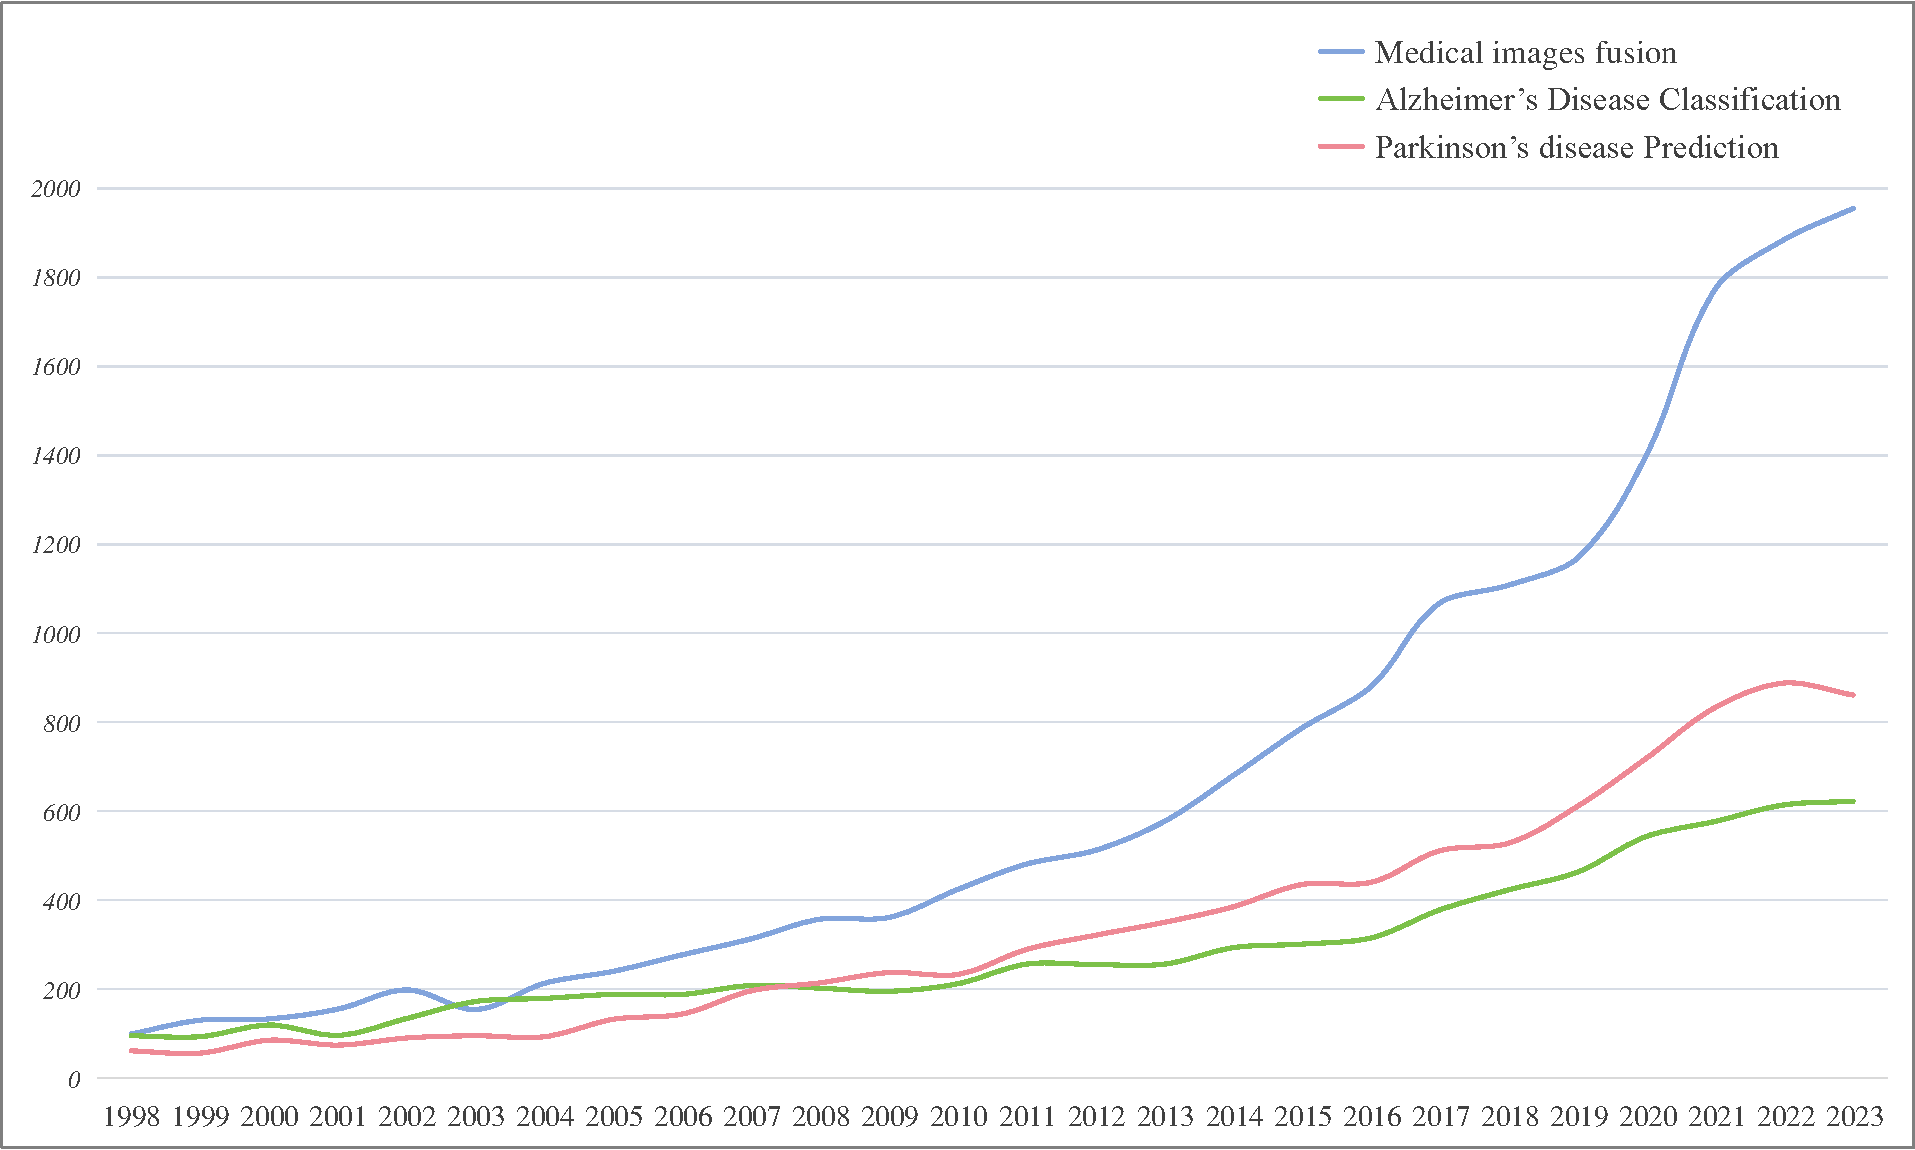
\includegraphics[width=0.9\linewidth]{figs/paperNumber.pdf}  
      \caption{按年搜索PubMed上三个关键词的发文量统计}\label{paperNumber}
    \end{figure}

基于智能辅助诊断的研究已经拓展至医学影像分析的多个领域,包括医学影像配准\cite{balakrishnan2019voxelmorph,ashburner2007fast}、医学影像分割\cite{sharma2010automated,zhou2018unet++,chen2021transunet}、医学影像融合\cite{anwar2018medical,dogra2023multi,tang2022image}、医学影像分类\cite{dai2021transmed,frid2018gan,wang2017chestx}、疾病检测\cite{gaitonde2017chronic,ferentinos2018deep}以及疾病预测\cite{dahiwade2019designing,shah2020heart,krishnamoorthi2022novel}等多个层面。将深度学习方法融入智能辅助诊断系统,
%不仅提高了诊断的准确性和效率,更为医学影像领域的发展注入了强大的活力,成为当前最具前景的技术路径之一。展望未来,随着技术的不断演进和深度学习算法的不断优化,我们有望目睹智能辅助诊断在医学领域发挥更为重要的作用。这
不仅将为医生提供更为准确、快速的诊断工具,也将为患者制定更加个性化和精确的治疗计划,推动医学影像技术不断走向新的高峰。
%因此,投身于深度学习方法在医学影像领域的研究与应用,将成为科技领域中最富有挑战性和前瞻性的研究方向之一。
本文将深入探讨多模态的医学影像融合、AD的影像分类及PD的疾病预测。图1.1统计了在PubMed上按年搜索“Medical images fusion”、“Alzheimer’s Disease Classification”以及“Parkinson’s disease Prediction”这几个关键词的文章数量,从中可以发现,在过去的25年里,基于智能辅助诊断的研究越来越受到关注。其中,多模态医学影像融合的研究正在以惊人的速度增长,其潜在的应用价值和社会影响不容小觑。

\subsection{多模态医学影像融合}
%随着影像处理技术的不断成熟和进步,影像融合技术正逐渐成为各个领域的研究热点,其中医学影像融合技术的崛起更是为医疗领域带来了全新的可能性。
在临床影像诊断中,医学影像融合技术能够将来自不同模态的医学影像(如CT、MRI、PET等)有效地融合,提供更全面、立体的信息,有助于医生更准确地诊断病变或异常情况。此外,医学影像融合还可以用于手术规划和导航,在手术过程中为医疗专业人员提供即时且高清的影像资料,旨在提升外科手术的精确性及保障患者的安全。在当前的研究中,医学影像融合算法主要分为基于传统方法和基于深度学习方法两大类别。


\subsubsection{基于传统理论的融合方法}
传统的医学影像融合方法涵盖了多种算法,其中包括基于稀疏表示\cite{liu2015general,maqsood2020multi,li2021medical}、基于形态学\cite{matsopoulos1994multiresolution,mukhopadhyay2001fusion,liu2019medical}、基于模糊理论\cite{ali2015multi,hu2021fuzzy,velmurugan2018multimodality}、基于多尺度分解\cite{jin2016medical,li2017pixel,singh2014fusion,yin2018medical}及基于机器学习的融合算法\cite{jasti2022computational,raja2020artificial,alseelawi2022novel,tang2019augmentation,diwakar2021latest}。
这些方法各自在不同场景下都表现出一定的优势,基于多尺度分解的融合方法由于其能够在不同尺度层面上进行信息处理,因而引起了广泛的研究兴趣。多尺度分解技术将影像转化为具有分层结构的多个尺度表示。这种分层结构的设计能在评估时兼顾影像的整体特性和具体细节,进而实现对影像深层意义的更全面理解。通过将影像分解成不同分辨率的子影像,多尺度分解允许独立处理不同层次的影像信息,有效地促进了对影像中关键特征的提取。这样的方法不仅有助于全局与局部信息的融合,还为影像处理提供了一种更为灵活、全面的手段,以适应不同尺度下的影像结构。基于多尺度分解的融合方法具备明显优势,能有效保留影像细节、融合全局与局部信息,同时增强特征表示,为影像处理任务提供强大支持。

拉普拉斯金字塔是典型的多尺度方法,特征金字塔的核心理念在于通过构建多尺度的影像表示,有助于系统更全面地理解影像中的对象特征,从而提升物体检测和识别的性能。Wang等人\cite{wang2011multi}将拉普拉斯金字塔变换的原理作为影像融合策略,该方法主要包括三个步骤
%,如图\ref{Pyramidfusion} 所示
。首先,分别对每个源影像进行拉普拉斯金字塔分解,然后采用不同的融合规则对新的每个拉普拉斯金字塔级别进行融合。对于最顶层,采用最大区域信息规则;对于其余级别,采用最大区域能量规则。最后,通过反向拉普拉斯金字塔变换得到融合影像。使用两组影像验证了提出的融合方法,并与其他融合方法进行比较。通过分析实验结果的分析显示,这种方法表现出了较好的性能,融合影像的质量优于其他方法的结果。
在医学影像融合领域,基于多尺度分解的方法通过将医学影像分解为不同尺度的子影像,分别进行处理并最终融合,以确保在整个处理过程中更好地保留影像的结构和细节信息。这种策略使得医生在进行临床诊断时能够获得更全面的信息,从而提高了对患者病情的准确评估。多尺度分解的融合方法在医学影像处理中的引入,强调了在融合过程中对影像多层次特征的关注,这种思想的实际应用在\cite{sahu2014medical,mi2021medical,jiang2023lightweight}等文章中大放异彩。
 \if 0
   \begin{figure*}[htbp]
      \centering
      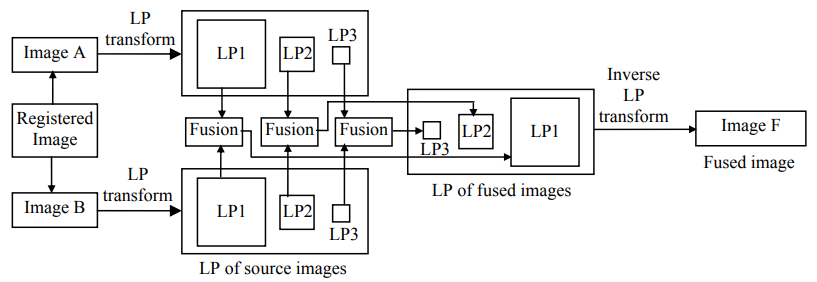
\includegraphics[width=0.95\linewidth]{figs/LaplacianPyramid.png}
      \caption{基于拉普拉斯变换的融合方法框架}\label{Pyramidfusion}
    \end{figure*}
  \fi

传统的融合方法中,医学影像融合通常依赖于人工设计的特征和规则,通过影像处理技术实现对不同模态医学影像的融合。这种方法在早期为医学影像的综合分析提供了基础,但受限于人工设计的特征和规则,其应用范围和效果逐渐受到限制。

\subsubsection{基于深度学习的融合方法}
近年来,随着深度学习技术的迅速发展,基于深度学习方法的医学影像融合技术\cite{rajalingam2018multimodal,liu2018deep,kaur2021multi,xia2019novel,zhou2023deep,rajalingam2022intelligent}取得了显著的突破。深度学习模型,特别是卷积神经网络(CNN)\cite{wang2020multi,el2021efficient,xia2019novel,li2021novel,zhang2023medical}以及生成对抗网络(GAN)\cite{zhou2023gan,huang2020mgmdcgan,ma2020ddcgan,wang2021dicyc}等,能够自动学习影像中的复杂特征和模式,从而实现对医学影像的更精细、准确的融合。这使得医学影像融合技术在影像诊断、手术导航等领域发挥着越来越重要的作用。

Lahoud等人\cite{lahoud2019zero}利用预训练神经网络,通过提取深度特征图进行影像融合,实现将来自多模态源影像的信息整合到单一输出中。与传统方法不同,该方法采用了新颖的策略,通过比较特征图生成融合权重,推动多模态影像的融合过程。这一方法不仅适用于两幅影像的融合,还可以扩展到任意数量的输入来源。实验证明,该技术在视觉质量、客观评估和运行效率方面均有较好的效果。Kaur等人\cite{kaur2021multi}提出了一种采用多目标优化策略结合深度学习的医学成像处理方法,实现了不同模态的医学影像之间的有效整合
%,如图\ref{fusionDL}所示
。该方法首先使用非子采样轮廓波变换(NSCT)将影像分解为子带。随后,采用Inception的极端版本(Xception)对源影像进行特征提取。使用多目标差分演化算法进行特征优化。之后,通过决定系数和一种基于能量损耗的融合策略来计算融合权重。最后,借助逆非子采样卷积变换构建融合后的影像。根据实验数据,这种方法在多模态影像融合技术中显示出明显的优势。
  \if 0
   \begin{figure*}[htbp]
      \centering
      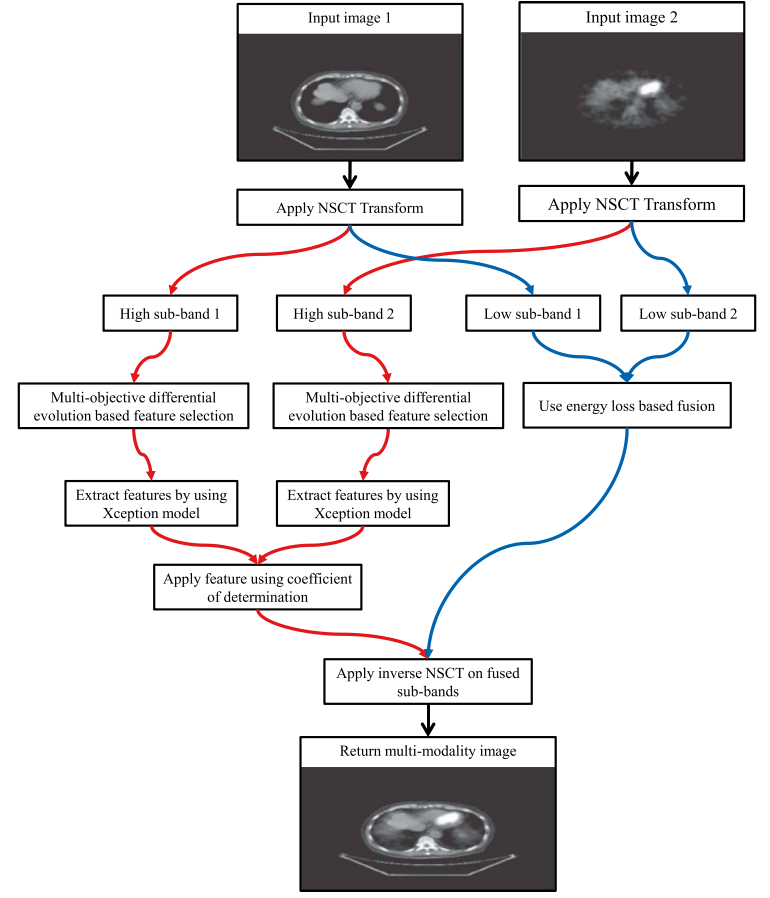
\includegraphics[width=0.95\linewidth]{figs/fusionDL.png}
      \caption{基于多目标差分进化的深度神经网络的多模态医学影像融合}\label{fusionDL}
    \end{figure*}
  \fi
  
Zhou等人\cite{zhou2023gan}总结了生成对抗网络(GAN)在深度生成模型领域的研究热点,特别是在医学影像融合方面的广泛应用。首先,从基本模型和训练过程两个方面阐述了GAN的基本原理;其次,将变种GAN模型总结为三个方向(概率分布距离、整体网络架构、神经网络结构),从基于f-散度的方法、基于IPM的方法、单生成器和双鉴别器GAN、多生成器和单鉴别器GAN、多生成器和多鉴别器GAN、条件约束GAN、卷积神经网络结构GAN和自动编码器神经网络结构GAN等八个维度总结了近年来的典型模型;第三,从三个方面探讨了GAN模型在医学影像融合领域的优势和应用;第四,介绍了GAN面临的主要挑战以及在医学影像融合领域所面临的挑战。
Ma等人\cite{ma2020ddcgan}介绍了一种带有双重鉴别器的条件式生成对抗网络(DDcGAN)框架,专门用于整合具有不同清晰度的红外与可见光图像。此模型利用生成器和两个鉴别器之间的对抗性互动机制,实现了在融合影像中同时保留红外影像的热辐射和可见影像的纹理细节。为了融合不同分辨率的源影像,DDcGAN采用降采样策略,以确保融合影像在保持信息清晰度的同时避免热辐射或纹理细节的丢失。该方法不仅在红外和可见光影像融合上表现出色,还在融合多模态医学影像方面取得了卓越的结果。

基于深度学习的医学影像融合不仅能够提高影像的清晰度和对比度,还能有效地在处理过程中维持影像的重要细节和内容,为医生提供更全面的诊断依据。此外,这些技术还有助于将不同模态影像之间的信息关联起来,为综合性医学分析提供更准确的数据支持。

\subsection{阿尔茨海默症的分类}
AD作为老龄化人群中常见的慢性神经系统退行性疾病,其主要特征表现为认知障碍和记忆缺失。由于其发病机制缓慢且目前难以完全治愈,早期发现和区分中度认知功能障碍(Mild Cognitive Impairment,MCI)和AD对于实施有效的干预和治疗至关重要。值得注意的是,MCI还分为两个亚型,即早期轻度认知功能障碍(Early MCI,EMCI)和晚期轻度认知功能障碍(Late MCI,LMCI),它们分别表示在认知功能下降中的不同阶段,EMCI通常早于LMCI发生。这样的细致划分对于更准确的病程分析和制定干预方案至关重要。然而,AD的影像诊断面临一系列挑战,因为实现精确分类依赖于能够明显区分不同类别的特征。诊断主要依赖于对患者脑部扫描影像的分析,涉及解决一个目标分类问题。由于脑部影像的微小差异和结构变化幅度相对较小,特征不够明显,如图\ref{fineAD},因此正确分类和判断阿尔茨海默症的病程变化具有较大难度。当前研究中,针对AD的影像分类算法主要分为两大类别:粗粒度分类(AD、NC和MCI这这种类别的2分类或者是3分类)和细粒度分类(早期分类,主要是将MCI细分成了EMCI好LMCI,再与AD或NC进行组合分类)。粗粒度分类主要关注整体疾病状态,而细粒度分类更注重对不同亚型的精准辨别。AD分类算法的发展旨在提高对MCI和AD的早期检测,以实现及时的干预和治疗,更好地预防或延缓疾病的进展。

   \begin{figure*}[htbp]
      \centering
      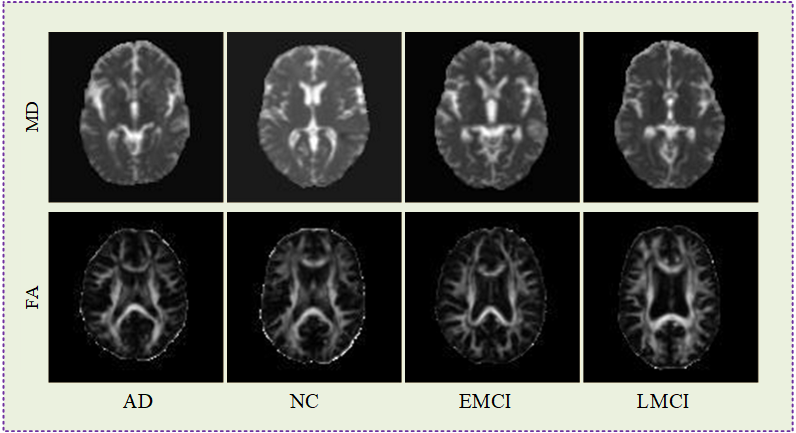
\includegraphics[width=0.9\linewidth]{figs/fineAD.png}
      \caption{四类(AD、 NC、EMCI、LMCI)受试者的两种DTI(弥散张量成像的分数各向异性(FA)和平均弥散率(MD))脑部影像}\label{fineAD}
    \end{figure*}
    
\subsubsection{基于粗粒度影像的分类应用}
本文探讨的问题是如何在AD、MCI以及正常对照组(Normal Control, NC)之间进行有效的分类。一些学者侧重于从脑部医学影像中抽取特定的AD病理特征进行分类\cite{gray2012multi,garali2015region,feng2021extracting,gray2011regional},例如海马、杏仁核及前额叶等关键脑区。Garali等人\cite{garali2015region}提出了一种新颖的方法,用于评估大脑区域在区分AD和健康脑影像方面的有效性。首先,将脑扫描数据分割并对齐至116个特定的解剖结构区域。然后计算这些区域的前四个时刻和直方图的熵。接着,使用接收器操作特性曲线对各个区域分离PET脑影像的能力进行排名。选取了21个区域作为输入,分别输入到支持向量机和随机森林分类器中,评估结果基于142个脑PET影像进行。分类结果较使用最初的116个区域或输入整个脑体素时更好。Feng等人\cite{feng2021extracting}提出了一种基于ROI的小波子带能量(ROICSE)特征方法,以在频域中表示sMRI影像进行AD分类。具体而言,sMRI扫描经过预处理步骤后,会使用预先定义的脑部掩膜进行分割,从而得到90个特定的兴趣区域(ROI)。与传统方法在空间维度上直接提取这些ROI特征不同,这里采用的是小波变换技术,对每一个ROI进行分析,从而获得其能量分布的不同子带。然后,对于一个ROI,构造一个子带能量(SE)特征向量来捕捉其能量分布和轮廓信息。随后,将90个ROI的SE特征向量串联起来形成sMRI影像的ROICSE特征。最后,使用支持向量机(SVM)将880名受试者的数据进行了分类,这些数据来源于ADNI和OASIS数据库。实验结果表明,AD vs. NC、MCI vs. NC和AD vs.MCI的准确率分别是93.57\%、83.13\%和82.73\%,ROICSE方法优于其他六种最先进的方法。Gray等研究者\cite{gray2011regional}将每位参与者的脑部MRI扫描细致地分割为83个不同的解剖部分。随后,他们使用这些解剖区域作为参考框架,从同个人的FDG-PET扫描中提取了各ROI的平均放射性标记强度数据。最终,通过分析这些强度值作为特征,利用SVM算法对样本进行了分类处理。在AD患者和NC对照组之间取得了出色的区分度(准确率82\%),在MCI患者和NC对照组之间取得了良好的区分度(准确率70\%)。
    \if 0
   \begin{figure*}[htbp]
      \centering
      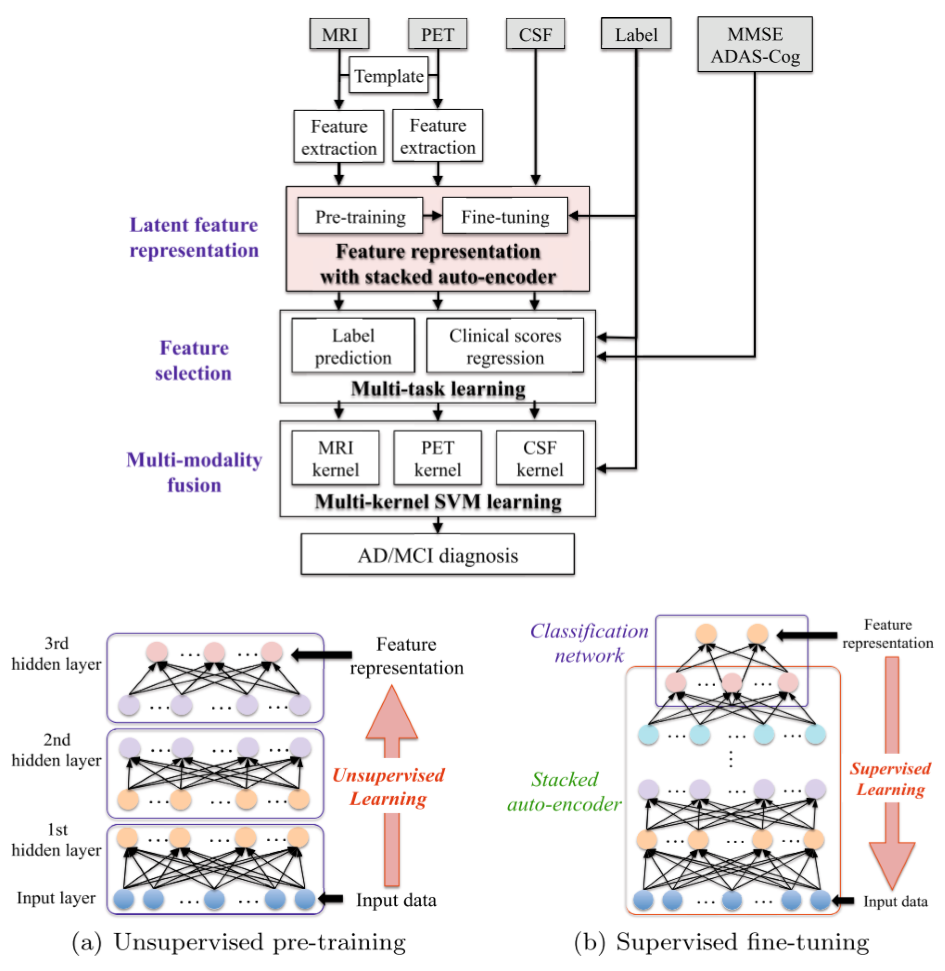
\includegraphics[width=0.95\linewidth]{figs/2classify.png}
      \caption{用于阿尔茨海默病的AD与MCI诊断的网络模型,潜在特征表示主要由堆叠自编码器(a)和两步参数优化方案(b)组成}\label{coarse2classify}
    \end{figure*}
    \fi
    
尽管基于特定区域的兴趣点的方法来提取关键特征并对这些特征进行深入分析的策略在某些方面表现出效力,但也存在一些明显的限制。首先,特征提取过程可能会受到人为因素的影响,导致错误,同时分析手段也可能存在局限性。由于AD标志物不明确,因此在划分和选择ROI时可能发生疏漏,极大地影响AD诊断的效果。再者,采用基于ROI的技术在实现时,模型训练通常需要依赖大规模的实验数据来保证预测结果的精确度,这无疑会增加显著的时间和人力资源消耗。而在阿尔茨海默病分类研究的现状下,采用ROI方法的研究者们普遍采取了多样化的影像预处理手段,包括但不限于影像与参考模板的精确对位、应用刚性或非刚性变换来适配不同的参照框架,以及对影像进行详细的区域分割处理。面对这些挑战,深度学习方法在AD影像分析中展现出卓越的潜力\cite{suk2013deep,so2019deep,suk2014hierarchical,tufail2021classification,khvostikov20183d}。深度学习通过学习数据中的特征,自动发现并表征影像中的复杂模式,避免了手动提取特征的繁琐过程。这使得深度学习在处理AD影像分类任务时更具优势。其对大规模数据的高效处理能力,以及在学习表征方面的卓越性能,使得深度学习方法成为应对上述问题的有力工具。

Suk等人\cite{suk2013deep}提出了基于深度学习的堆叠自编码器的特征表示方法
%,如图\ref{coarse2classify}所示
。为了创建一个可靠的AD/MCI分类模型,作者综合考虑了深层信息和基础特征,以此提高模型的诊断性能。实验证明,所提出的方法对于AD、MCI的诊断分别具有95.9\%、85.0\%的准确率。通过对训练模型的可视化观察,一种利用深度学习技术来获取神经影像数据中高级共享潜在特征的新方法被提出\cite{suk2014hierarchical}。具体而言,该框架以受限的玻尔兹曼机(DBM)为单元,能够从三维图像片段中识别并提取层次化的潜在特征。接着,应用多模态DBM对MRI和PET图像的对应区块进行了联合特征提取。为了评估所提出的方法的效能,进行了一系列详尽的实验测试,并与最先进的方法进行了比较。在AD vs. NC、MCI vs. NC分类问题中,分别获得了95.35\%、85.67\%的最大准确率,优于竞争方法。
So等人\cite{so2019deep}提出了一种结合纹理分析与深度学习的AD粗粒度分类方法。首先对MRI影像应用了三维灰度共生矩阵(GLCM)方法进行纹理分析。然后,使用Fisher系数选择适用于分类的特征。最后,利用多层感知器(MLP)模型将其分为AD vs. MCI、AD vs. NC和MCI vs. NC三类。该模型在分类准确性上表现出色,分别为AD vs. MCI(72.5\%)、AD vs. NC(85\%)和MCI vs. NC(75\%),并在混淆矩阵、支持向量机(SVM)和K最近邻(KNN)分类器的评估中展现出优越性。所提出的方法相较于SVM和KNN分类器至少提高了6-19\%的准确率。自动化的AD分类系统可以作为辅助工具,帮助医务人员诊断阿尔茨海默病的阶段,从而提供适当的医疗治疗。 
Khvostikov等人\cite{khvostikov20183d}提出了一种基于3D Inception的卷积神经网络(CNN)的设计,用于AD的诊断。该网络注重内部资源的利用,通过在海马ROI上融合sMRI和DTI模态。与传统的基于AlexNet的网络相比,表现显著更好。AD vs. MCI vs. NC、AD vs. NC、AD vs. MCI与MCI vs. NC这些分类的准确率分别是68.9\%、93.3\%、86.7\%和73.3\%。

%从脑部医学影像中抽取特定的AD病理特征诊断的方法相对基于深度学习诊断的方法精确度略低。但,关于AD的粗粒度分类问题主要包括二分类(AD vs. NC、AD vs. MCI和MCI vs. NC)或三分类(AD vs. MCI vs. NC),无法辅助诊断更进一步的多阶段。
尽管在脑部医学影像中提取特定的AD病理特征的方法在精确定位疾病迹象方面取得了一定的成果,然而,与那些依赖深度学习的诊断技术相比,这些传统方法在精确度上稍显不足。这可能是因为这些传统方法主要关注单一或少数感兴趣区域(ROI),而对于复杂的神经影像数据,这种精细的特定特征提取方式难以涵盖疾病的整体情况。
特别是在处理AD的粗粒度分类问题时,通常涉及二分类(AD vs. NC、AD vs. MCI和MCI vs. NC)或三分类(AD vs. MCI vs. NC)的任务。这些任务主要旨在初步判别患者的整体状态,而未能提供关于疾病进展更详细信息的细致分析。相比之下,基于深度学习的方法通过学习大量数据中的特征,具有更强大的表示学习能力,可以更全面地捕捉疾病的复杂模式和变化。
这种方法的优势在于其对大规模和多模态数据的高效处理,以及对于特征学习的自动化处理。这种自动化处理避免了手动提取特征时可能引入的主观性和繁琐性。因此,基于深度学习的方法展现出更高的潜力,有望推动AD诊断领域向更为准确和全面的方向发展。这不仅提供了更有力的支持,还有助于更全面地理解和干预AD等神经系统疾病的发展过程。
    
\subsubsection{基于细粒度影像的分类应用} 
尽管AD的粗粒度分类方法在筛查、早期检测和初步诊断方面具有一定的实用性,对于医务人员而言,在多阶段AD的诊断中进一步了解疾病的不同阶段、进展速度以及相关病理学变化,对个体化的治疗方案和干预手段更具有指导意义。目前,关于AD的智能辅助诊断的研究在多个AD进行性阶段方面的适用性相对较少。近年来,越来越多的学者对AD进行了细粒度的研究,例如\cite{korolev2017residual,ruiz20203d,song2019graph,parmar2020spatiotemporal,pan2020early,basaia2019automated,helaly2021deep,fu2021automated,shamrat2023alzheimernet}等。

Korolev等人\cite{korolev2017residual}采用残差网络和普通3D卷积神经网络结构,应用于3D结构性MRI脑扫描的AD与MCI以及NC的分类任务中,涉及到AD与NC、EMCI、LMCI之间的多类别分类。该研究展现了在细粒度分类上的一定成果,不仅涉及AD vs. NC,还包括了AD vs. EMCI、AD vs. LMCI、LMCI vs. NC等任务,其结果表明了模型在处理这些复杂分类问题上的鲁棒性。实验测试的准确率分别是:AD vs. NC: 80\%,AD vs. EMCI: 63\%,AD vs. LMCI: 59\%,LMCI vs. NC: 61\%,LMCI vs. EMCI: 52\%,EMCI vs. NC: 56\%。
Ruiz等人\cite{ruiz20203d}则提出了一种集成方法,采用3D密集连接卷积网络(3D DenseNets)模型进行四分类,即AD、EMCI、LMCI和NC。这种方法通过密集连接改善模型内部数据的流动,同时采用概率融合方法合并每个独立分类器模型的概率输出。在测试中,该方法相对于处理3D MRI的其他最新方法表现更好,获得了66.67\%的准确率,为细粒度分类提供了可行的解决方案。
    
Song等人\cite{song2019graph}使用图卷积神经网络(GCN)进行网络分类,将受试者分为NC、EMCI、LMCI和AD四个类别,实现了89\%的准确率。Parmar等人\cite{parmar2020spatiotemporal}通过使用经过修改的3D卷积神经网络设计了一种简化而准确的方法,从静息状态fMRI数据中提取特征并对AD进行四分类。该研究中的CNN设计保留了更多的空间和时间信息,获得了93\%的准确率,为对AD进行多阶段诊断提供了一种潜在的有效途径。
Helaly等人\cite{helaly2021deep}则采用两种基于深度学习的方法对医学影像进行AD四个阶段(AD vs. EMCI vs. LMCI vs. NC)的分类。这两种方法分别基于简单的CNN架构和迁移学习原理,使用不同的模型进行医学影像分类。具体来说,第一种方法使用简单的CNN架构,该架构基于2D和3D卷积处理数据集为2D和3D的脑部扫描。第二种方法应用迁移学习原理,利用预训练的模型(VGG19模型)进行医学影像分类。这两种方法分别取得了93.61\%和95.17\%的准确率,为多阶段AD分类提供了更多选择。
 \if 0
   \begin{figure*}[htbp]
      \centering
      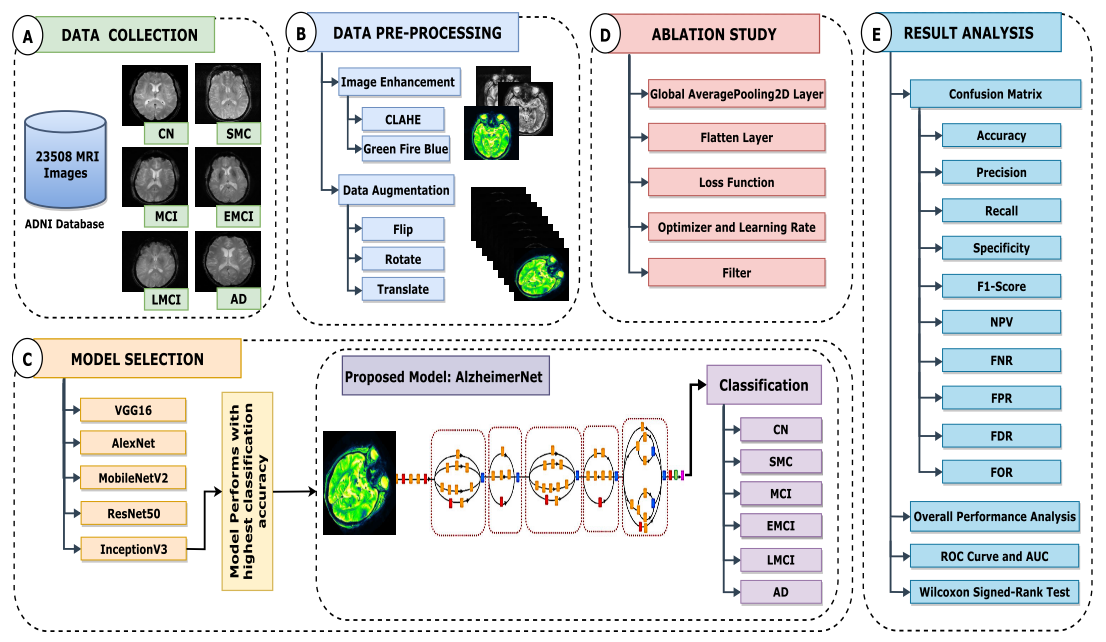
\includegraphics[width=0.95\linewidth]{figs/5classify.png}
      \caption{用于阿尔茨海默病的多分类(SMC、AD、NC、MCI、EMCI、LMCI)的网络模型(AlzheimerNet)结构}\label{fine5classify}
    \end{figure*}
 \fi
 
少数研究还对AD的进行性阶段(包括NC、主观记忆问题(SMC)、EMCI、MCI、LMCI和AD)进行了多类别分类\cite{shamrat2023alzheimernet,ramzan2020deep},进一步拓展了对AD多阶段的认知。Shamrat等人\cite{shamrat2023alzheimernet}提出的AlzheimerNet分类器具有更细致的多阶段诊断能力
%,分类器结构如图\ref{fine5classify}所示
。通过精细调整的卷积神经网络(CNN)架构,该模型可以识别阿尔茨海默病的五个阶段,包括SMC、MCI、EMCI、LMCI和AD以及NC类别。在六分类任务上,通过比较五个预训练模型(VGG16、MobileNetV2、AlexNet、ResNet50和InceptionV3)和AlzheimerNet模型在各种性能指标上的表现,该模型表现出98.68\%的准确率,显示出了在多阶段AD诊断中的出色性能。

在AD的细粒度分类方法中,主要集中在二分类任务,例如AD与EMCI、AD与LMCI、LMCI与NC、LMCI与EMCI等。这些二分类任务在当前研究中占据主导地位,主要受到深度学习方法的广泛运用。就二分类而言,研究结果表明,这些方法在AD的早期诊断、疾病阶段划分以及患者与正常对照的区分等方面取得了显著的成果。例如,Korolev等人\cite{korolev2017residual}在AD vs. NC、AD vs. EMCI、AD vs. LMCI等任务中实现了可观的分类准确性,为早期AD的精准辨别提供了可能性。相比之下,三分类任务(如AD vs. EMCI vs. LMCI、NC vs. EMCI vs. LMCI)相对较少,研究涉及更多的类别,需要更高的分类难度和挑战。在这方面,尚未形成广泛的研究共识。

然而,一些初步的研究显示,在处理多类别分类问题时,模型的性能仍然具有潜在的优势。通过更全面的分类,有望提供更丰富的信息,为医务人员提供更全面的诊断参考。
六分类任务,涉及到NC、SMC、EMCI、MCI、LMCI和AD的分类,是相对较少见的研究方向。在这一领域,Shamrat等人\cite{shamrat2023alzheimernet}提出的AlzheimerNet分类器在实现六分类任务上表现出色,具有98.68\%的准确率,显示了对多阶段AD进行细致分类的强大潜力。这种细粒度的多分类方法有望为医疗决策提供更详细的信息,推动个体化治疗和干预的发展。
绝大多数采用深度学习方法的AD细粒度分类方法,其准确率存在一定的差异,取决于模型的架构设计、数据集质量以及训练过程中的参数调整等因素。在这方面,不同的研究方法可能呈现出高低不一的性能。然而,总体趋势显示出深度学习方法在解决AD细粒度分类问题上的潜在优势,通过学习丰富的影像特征,更全面地捕捉疾病的多样性,为提高AD诊断的准确性和全面性提供了有效途径。


\subsection{帕金森疾病的预测}
帕金森症(PD)是一种长期性的神经退行性疾病,它直接作用于那些在大脑中制造多巴胺的关键神经元。这种疾病在神经系统疾病中的发病率排在第二位,仅次于AD\cite{prusiner2001neurodegenerative,leroy1998deletions}。
许多患有PD的患者在被诊断时已处于病情的中到晚期阶段,这使得他们失去了接受最佳治疗的理想时机。\cite{de2019prognosis,papagno2018cognitive}。因此,急需开发出更快捷、更精确、更具效能的检测技术,以便实现对PD的早期识别\cite{jyWen}。可作为PD预测的数据主要包括医学影像数据和临床数据。
医学影像数据可以呈现出脑部结构和活动的直观影像,有助于观察神经元损伤和多巴胺生成的变化。临床数据则提供了更全面的患者信息,包括症状描述、家族病史以及其他相关的临床特征,这些信息对于全面评估患者的健康状况至关重要。
将医学影像数据和临床数据相结合,可从多个角度来分析和理解帕金森病的发病机制,从而构建出更精确、更可靠的早期诊断模型。这样的模型不仅能提高诊断的准确性,还能为患者提供及时的治疗建议,提升生活品质并减缓病症进展。

\subsubsection{基于医学影像的预测方法}
在医学影像学领域,不断涌现新技术以助力帕金森病(PD)的诊断。这些技术因其独特的优势而备受瞩目,预计将大幅提升诊断的准确性。医学影像学提供了多种影像类型,如磁共振成像(MRI)揭示了大脑结构的细微差异;功能性磁共振成像(fMRI)捕捉了脑部活动模式;结构磁共振成像(sMRI)评估了大脑组织的形态改变;单光子发射计算机断层扫描(SPECT)和正电子发射断层成像(PET)则用于检测大脑代谢异常;弥散张量成像(DTI)描绘了神经纤维束的走向和完整性。这些技术共同为PD的早期发现与治疗提供了强有力的工具。


基于体素的形态测量学(voxel-based morphometry,VBM)技术利用MRI扫描快速且精确地量化脑部形态变化,如小脑的体积减少,并能在宏观层面迅速定位帕金森病(PD)的脑结构异常\cite{li2018patterns,de2017loss}。这项技术在成本效益和诊断准确性方面表现出色,已被临床研究所证实。Amoroso等学者\cite{amoroso2018complex}通过分析大脑肌肉萎缩与疾病严重度的关系,创建了一套全面的脑结构网络模型,其疾病分类准确度超过了94\%,优于标准VBM分析。另外,Rojas等人开发了一种基于SPECT影像的经验模式分解新技术\cite{rojas2013application},结合PCA提取关键特征并运用SVM进行分类,实现了高达95\%的准确率。Alexandra等人\cite{abos2017discriminating}通过对两组独立的受试者的静息态功能磁共振影像进行分析,并运用随机逻辑回归挑选特征输入SVM,在测试集中达到了80\%的预测准确率。

Francisco等研究者\cite{oliveira2018extraction}开发了一种新技术,通过分析FP-CIT SPECT影像来预测PD,并通过运用支持向量机(SVM)、K最近邻(KNN)以及逻辑回归这三种不同的机器学习模型,实现了97.9\%的高分类精度。此外,Martinez等人\cite{martinez2018convolutional}采用FP-CIT SPECT的医学影像数据结合CNN架构,包括LeNet3D与Alexnet3D,对PD进行了分类,其中Alexnet3D的分类准确度为94.1\%,曲线下面积为98.4\%。Kim等人\cite{kim2018artificial}应用了Inception V3网络进行PD预测,获得了87\%的曲线下面积。Castillo等人\cite{castillo2018robust}提出了一个集成学习的分类模型,结合了SPECT影像数据和多种生物学标记,构建了一个加权分类模型,该模型的分类准确度为96\%。这些研究成果显示,利用医学影像数据的PD预测技术正在持续改进,这些技术不仅提高了预测的准确性,还引入了多种先进技术和深度学习框架,为PD的早期诊断提供了更稳健和精确的工具。


\if 0
   \begin{figure*}[htbp]
      \centering
      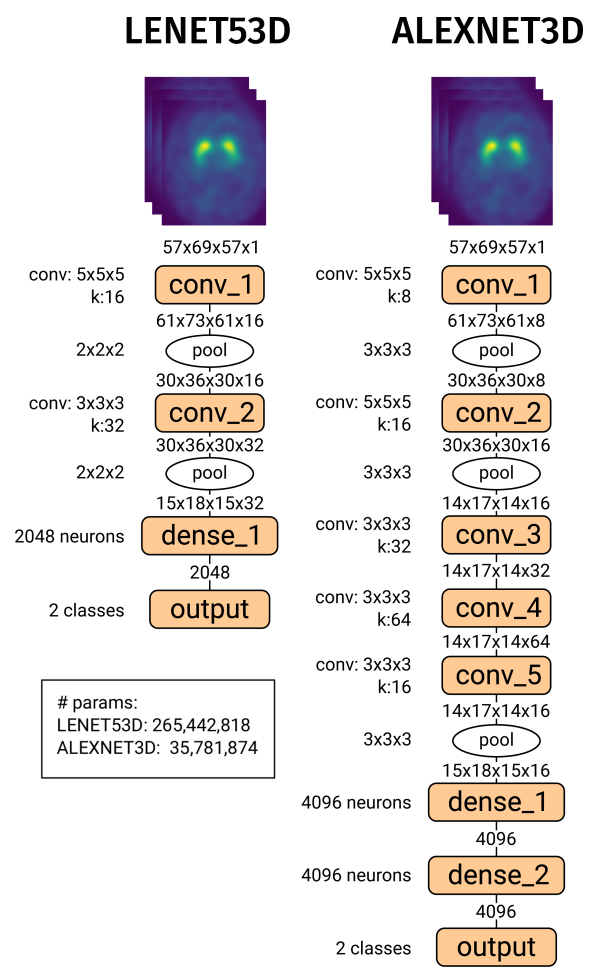
\includegraphics[width=0.8\linewidth]{figs/imagePredict.png}
      \caption{Lenet53D和Alexnet3D网络模型结构\cite{martinez2018convolutional}}\label{prePDimage}
    \end{figure*}
\fi    


近期研究通过DTI技术深入分析了患者的症状,进一步揭示了白质网络中神经元损伤的情况,并将其与正常对照组进行了比较。结果显示,PD和MCI患者的额叶白质网络功能损伤较为集中,且认知网络的全面功能失调和多个神经元认知网络在频率域内所表现出的功能损伤之间存在直接联系\cite{wang2020changes}。
多模态MRI数据融合了磁共振成像的特点与早期疾病检测的优势,为PD的早期发现提供了有价值的影像学生物标志物\cite{jyWen}。尽管sMRI和DTI单模态技术能够较好的反映血脑网络的宏观结构变化,但它们在功能形态层面上仍有不足。Rs-fMRI主要用于评估缺血性痴呆患者的脑灰质异常,但目前尚未能够全面且系统地评估其对脑白质异常所导致的神经元活动失常以及相关的脑功能变化和特征\cite{jyWen}。此外,针对大脑黑质皮层区域,现有的磁共振扫描成像技术也存在一定的局限性。尽管对该区域的异常表现具有较高的灵敏度,但在描述这些特征时仍然面临着复杂性、模糊性以及单一性的问题。

为了克服这些技术挑战,研究者们开始采用多模态检测和多重MRI异常检测技术,融合多种特征进行综合分析。该方法通过多角度、多层次地分析PD的神经病理状况,实现了对疾病的全面诊断及治疗效果的综合评价。它为中国PD神经病理学的临床诊断和评估提供了一个较为完善、成熟、合理且可靠的新途径\cite{pyatigorskaya2018comparative,gu2016automatic,bowman2016multimodal}。Pyatigorskaya等人\cite{pyatigorskaya2018comparative}首个遵循国际准则对NMS-MRI信号进行详尽剖析的工作,旨在揭示黑质中的质子体积与信号强度的特定特征,并在DTI技术支持下,分析了局部各向异性的特性及其信号组合模式。成功将PD的预测准确率提升至93\%。Bowman等人\cite{bowman2016multimodal}则采用融合的策略,并分析和讨论了rs-fMRI、sMRI以及DTI中的组织结构特性。
经综合考虑多种影像学指标如灰质密度、各向异性分数和功能连接等,以区分PD患者与正常对照组。通过这种多模态分析方法,他们达到了98.9\%的分类准确率,这一结果显著优于仅依赖单一影像模态的传统方法。这些发现不仅增强了对PD神经生物学特征的理解,而且为临床上PD的早期识别和治疗策略的制定提供了重要的影像学参考。

在医学影像领域,针对PD的早期诊断技术正在不断进步,涵盖了包括sMRI、扩散张量成像(DTI)和静息态功能磁共振成像(rs-fMRI)在内的多种成像手段。这些技术能够揭示出具有高度特异性的影像学生物标志物,从而增强了对PD早期阶段的识别能力。尽管如此,每种技术也面临着自身的挑战;例如,sMRI和DTI在捕捉功能性形态变化方面存在不足,而Rs-fMRI在评估脑白质皮层异常的神经元变化时则可能受到限制。为了克服这些限制,研究者们开始探索多模态检测和多重MRI异常检测技术的应用。这种方法通过综合不同MRI技术的优势,从多个维度和视角对PD进行全面的临床诊断和疗效评估。现有的研究\cite{pyatigorskaya2018comparative,gu2016automatic,bowman2016multimodal}表明,这种多模态方法能够取得较高的预测准确性,为我国在PD神经病理学临床诊断评估指标方面提供了新的思路和方法。


\subsubsection{基于临床数据的预测方法}
医学领域的临床资料丰富且多元,为深入研究PD提供了宝贵资源。临床资料广泛涉及病患的生理和生化指标,其中蕴藏着揭示PD特征的关键信息,对于预测PD的发展趋势具有重要价值。基于这些临床数据的PD预测方法,对于指导医学实践和治疗方案的制定具有重要意义。

在认知障碍领域,PD患者常伴有帕金森病痴呆(Parkinson’s disease dementia,PDD),及时识别其进展对患者的治疗和生活质量具有重大影响。为此,Kim等人\cite{kim2019prediction}采用了三种常用的认知评估测评——蒙特利尔认知评估(MoCA)、马蒂斯痴呆分级量表(DRS-2)和简易的精神状态测评表(MMSE),并使用回归模型评估了它们在预测PD认知进展方面的效能。研究发现,在条件一致情况下,MoCA在诊断PD轻度认知障碍(PD-MCI)和PDD方面的准确性最高,分别达到了AUC=0.79和AUC=0.89,敏感性分别为76.4\%和81.0\%。这一成果首次证明了MoCA可以作为预测PDD发生的指标。尽管MoCA在检测和预测PD-MCI和PDD进展方面获得了较好的应用\cite{hu2014predictors,pigott2015longitudinal,marras2013measuring,hoops2009validity,dalrymple2010moca},但MoCA的低特异性限制了它作为诊断工具的实用性\cite{marras2013measuring,hoops2009validity},这反映了PD进展的复杂性以及当前缺乏可靠的客观生物标志物\cite{miller2015biomarkers}。因此,开发更先进的PD进展预测模型或更精确的诊断策略,对于选择合适的临床试验参与者显得尤为重要。

随着海量数据集的涌现,特别是那些涵盖纵向研究和多维度信息的数据集\cite{latourelle2017large,simuni2016predictors,holford2006disease},为PD进展预测模型的构建迎来了新的发展契机。例如,Diba等研究者\cite{ahmadi2019parkinson}通过机器学习技术分析PD的血清样本的研究,揭示了外周炎症标志物与PD症状间的联系。研究结果表明,患者初始阶段的外周炎症水平对于预测其病情的未来演变具有重要意义。Chan等人\cite{chan2007levodopa}提出的预测模型,证实了诸如左旋多巴之类的药物在控制PD发展和改善患者症状方面的显著疗效。
也有学者利用生物力学测量,包括步态和姿态的平衡能力,构建了预测PD患者两年之内进展的网络模型\cite{raval2020prediction},该模型采用CNN技术预测MDS-UPDRS第三部分评分的两年变化率,为针对快速进展型PD的药物治疗提供了新思路。
另外,Latourelle等人\cite{latourelle2017large}的研究指出,临床基线的运动评分数据是预测PD未来发展速度的关键因素之一。

在PD的初期阶段,及时检测非运动症状对于控制病情发展极为重要。Nilshi及其同事\cite{nilashi2020remote}开发了一种新的远程监控PD进展的技术,该技术融合了深度学习与聚类分析两种方法。具体实施时,研究团队采用了深度信念网络(DBN)结合支持向量回归(SVR)的策略来预测PD的UPDRS评分,并构建了多个时间尺度上的DBN预测模型。为了提升预测的性能,研究中还引入了自组织映射(SOM)的聚类技术,并通过SVR对DBN模型的预测结果进行整合优化。研究成果表明,这种结合聚类与DBN,再通过SVR进行结果融合的方法,在预测Total-UPDRS和Motor-UPDRS方面均优于单一的SOM、DBN或SVR技术。具体而言,在预测Total-UPDRS时,测试集上的均方根误差(RMSE)与决定系数(R2)分别达到了50.8\%与93.3\%;在预测Motor-UPDRS得分方面,模型的均方根误差(RMSE)为52.1\%,决定系数(R2)则达到91.4\%。这一技术开辟了远程监控PD患者病情进展的新途径。

在医学研究领域,对PD的多样化临床数据进行深入分析,是揭示疾病预测因素的关键。当前研究重点之一是对比不同的认知评估测试,其中蒙特利尔认知评估(MoCA)在检测PD认知障碍方面显示出较强的能力,尽管如此,其低特异性问题仍待克服。结合大型数据集及ML技术,PD的进展预测模型得到了显著提升,特别是在生物标志物和基因与疾病关联的探索上。总体来看,PD的研究正步入充满希望的新阶段,为更有效的疾病干预和治疗策略提供了坚实的科学支撑。

    
\section{本文的主要工作}
本项研究聚焦于智能辅助影像组学分析技术在医学辅助诊断领域中的应用,特别关注脑肿瘤、AD和PD。关键技术手段涵盖影像融合、影像分类与疾病预测。本文的主要工作包括:
\begin{itemize}
    \item 在多模态医学影像融合方面,本文分析了MRI、CT、PET、SPECT及其他医学影像,归纳总结了其各自隐藏的医学语义信息,并与影像特性对应,设计了一个医学语义引导的双分支网络。另外,本文从多个维度如低频、高频和多尺度出发,分析不同的空间、通道特征,提出三种特征提取模块。并结合自适应线性融合策略,提出一种多模态脑影像融合的网络模型。这两种方法都得到了临床医师较高的评价。
    \item 在AD诊断方面的研究上发现了AD不止有三类(AD、NC和MCI),其中MCI还可以分期,细分为EMCI和LMCI。EMCI阶段是可逆的,及时发现和干预可以避免AD的发展,而在LMCI阶段及时诊断和治疗可以延缓AD的发展或治愈AD。另外,由于绝大多数基于深度学习方法的应用都难于获得全局的特征,而频域的处理可以做到。因此,本文提出了一种小波卷积单元,并将其应用于AD的细粒度多分类。
    \item 在PD诊断领域,本文归纳总结了现阶段国内外学者在PD预测上的研究工作,将其定义为静态和动态预测两种类型。针对当前的研究现状,本文讨论和分析了PD智能诊断未来的研究趋势。另外,本文在PD基线的跨模态(除了考虑影像层面的数据外,还结合了非影像类数据)数据中,筛选了代表PD进展的关键特征。其次将跨模态的数据融合,应用于PD的进展预测,并提出了一种跨模态融合预测进展的方法,有利于临床预测性能的提升。
\end{itemize}


本研究课题内的各工作环节间存在着紧密的相互联系与支撑。首先,通过引入首个关于多模态医学影像融合的任务,确立了医学语义的核心概念,这一理念继而被融入第二个融合方法中,显著增强了影像的可解释性,为病灶的精确定位与动态追踪提供了有力支持。在实施这两项多模态融合技术的同时,现有神经网络模型在捕获全局特征方面的局限性被意识到,进而促成了第三个工作——即通过优化网络结构以有效拓展感受野,并成功应用于AD的细粒度分类,实现了诊断精度的新突破。
进一步地,本文巧妙地将多模态影像融合的思路迁移至跨模态数据融合的领域,特别是在帕金森病(PD)病情进展预测的研究中,这一思路的应用极大提高了预测的准确性。综上所述,这些工作的依次开展不仅在技术层面上形成了层层递进的创新链,还拓宽了技术应用范围,共同促进了智能辅助影像组学技术的发展与临床价值提升。


   \begin{figure}[ht]
      \centering  
      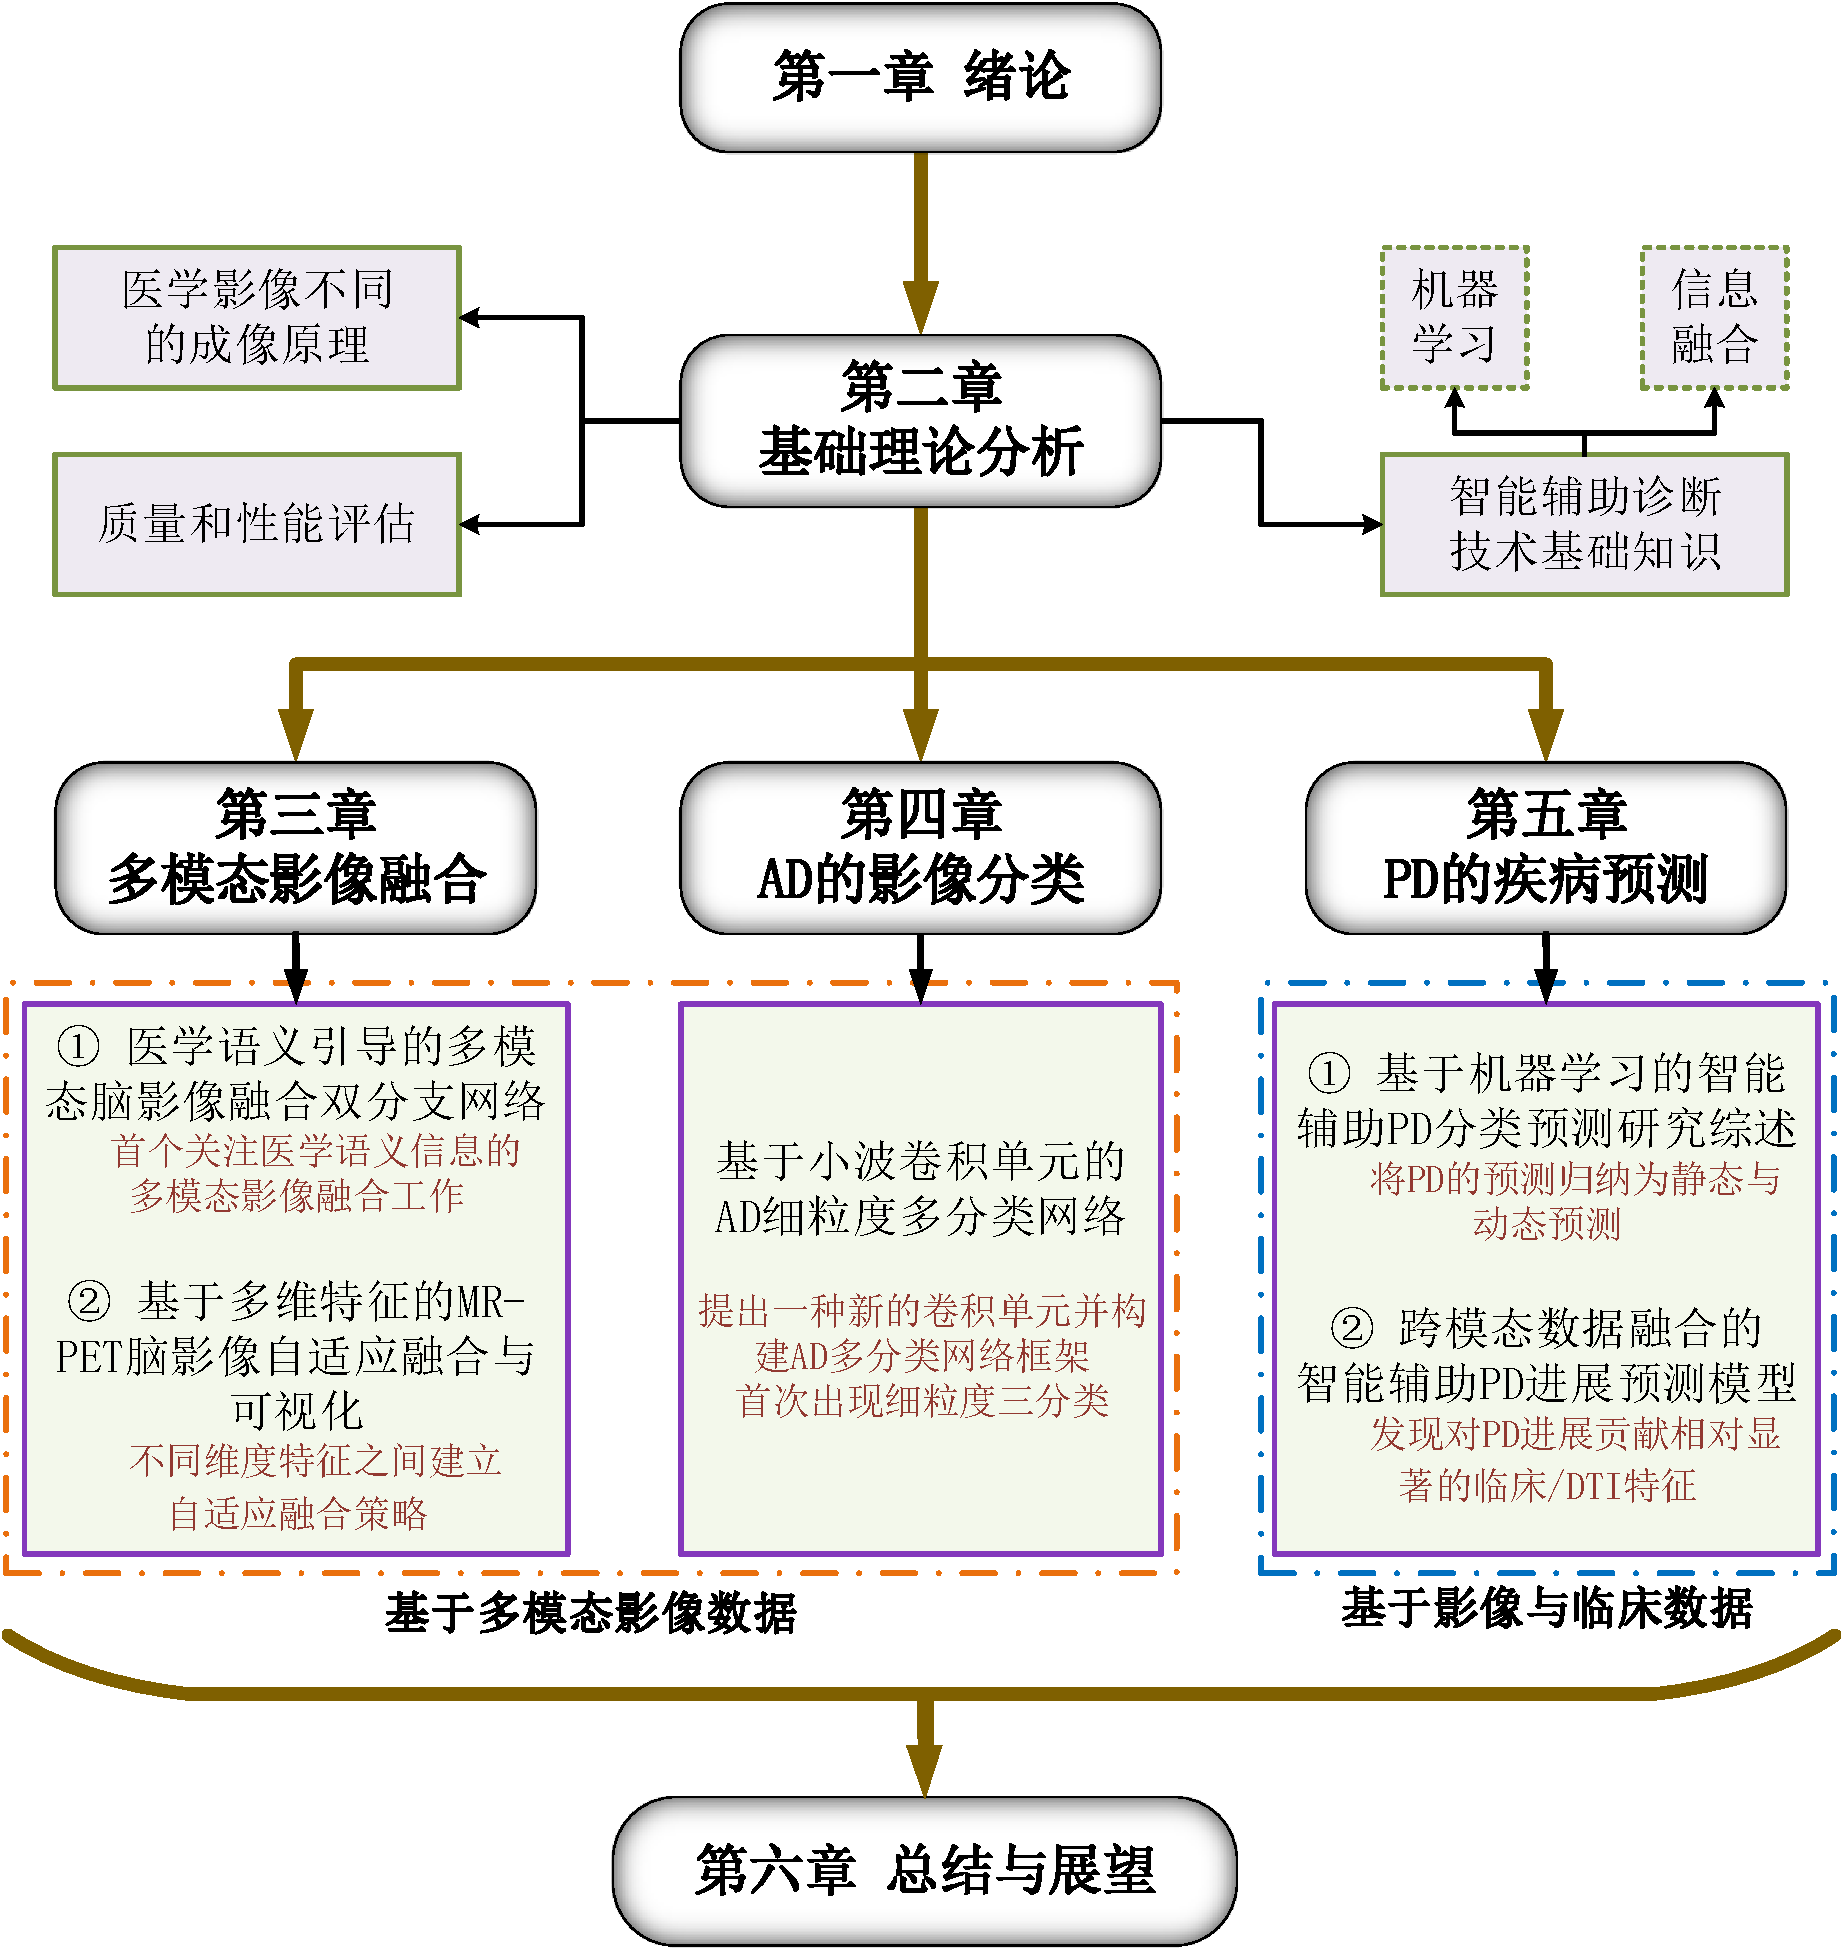
\includegraphics[width=0.88\linewidth]{figs/wholeWork.pdf}  %wholeWork.png
      \caption{本研究的内容布局与章节安排}\label{wholeWorks}
    \end{figure}

%\section{本文的篇章结构}
全文共分为六个章节,整体的篇章结构如图\ref{wholeWorks}所示。
   
第一章绪论。本章深入介绍了基于医学影像组学的智能辅助技术的研究背景与意义。强调了基于医学影像组学的智能辅助诊断技术的关键任务,包括影像融合、影像分类与疾病预测等方面。具体而言,本章详细分析了国内外在多模态医学影像融合方面的研究,包括基于传统方法和深度学习方法的不同取向。此外,本章对AD影像分类进行了深入讨论,涵盖了粗粒度分类(AD、MCI、NC的二分类或三分类)和细粒度分类(AD、EMCI、LMCI、MSC、MCI、NC的二分类、四分类和六分类)。最后,本章聚焦于PD预测,探讨了基于影像数据和基于临床数据两个层面的研究现状。整体而言,该章节不仅对研究内容进行了明晰概述,还为后续章节的深入探讨奠定了坚实基础。
    

第二章基础理论。本章深入研究了医学影像的多模态特性,对不同类型的医学影像成像技术原理进行了详细介绍,包括CT、MRI、PET等。本章详细分析了智能辅助诊断技术的理论基础,涵盖了传统机器学习方法(如SVM)和深度学习方法(如CNN)在医学影像分类中的应用。强调了这两者的融合是提高医学诊断准确性和效率的前沿趋势。另外,本章着重考虑了多模态数据的复杂性,讨论了信息融合的策略,包括像素级、特征级和决策级的融合方法,为实际应用提供了有益的启示。最后,本章还介绍了多种质量评估指标,包括主观与客观评价方法。对于有关医学影像基础理论和信息融合策略的全面认识,为后续章节中的具体技术方法提供了理论指导。


第三章聚焦于多模态影像融合。设计了两种新型的结合两种医学成像技术的融合方法,以实现更全面的信息整合。
一种是名为MsgFusion的基于医学语义信息(MS-Info)引导的融合方法。通过分析MR/CT/PET/SPECT的关键MS-Info,该方法获取相应的影像特征,采用SF分支和GV分支的双分支网络,成功提高了CNN的泛化能力。在医学脑影像的处理和分析中,包括MR-CT影像融合、MR-SPECT影像融合和MR-PET影像融合等方面,该方法相较于现有方法表现出显著优势,得到了临床医生的高度评价和统计数据的支持。
另一种也是基于深度学习的融合框架。它结合了多维特征、空间特征和通道特征,并引入了三种不同的特征提取模块(粗特征模块(coarse feature module,CFM)、精细特征模块(coarse feature module,FFM)和多尺度特征模块(multi-scale feature module,MFM))和自适应线性融合机制。该方法还提出了一种关键特征增强策略,可以增强同一病例不同时期融合影像的可视化效果,有助于肿瘤定位、分割和疾病跟踪等临床应用。
%基于本章的主要研究成果“MsgFusion: Medical Semantic Guided Two-Branch Network for Multimodal Brain Image Fusion”已在SCI Top期刊《IEEE TRANSACTIONS ON MULTIMEDIA》上刊载;“High-Quality Fusion and Visualization for MR-PET Brain Tumor Images via Multi-Dimensional Features”已收到SCI Top期刊《IEEE TRANSACTIONS ON IMAGE PROCESSING》的录用通知。


第四章关注AD影像分类。首先,提出了一种创新的卷积单元(wavelet convolution unit,WCU),它将小波变换与传统卷积函数结合,以获得更广泛的非局部感受野,显著提升卷积神经网络性能。在WCU的引导下,本章设计了影像分类的网络框架(WCU-Net)成功应用于AD的细粒度和多分类任务。基于AD的脑DTI数据(NC、MCI、EMCI、LMCI、AD)实现了所有粗粒度和细粒度的12种组合分类,包括首次引入的细粒度三分类。该框架在所有12种分类中取得了高准确率,尤其在8种细粒度分类中表现卓越。细粒度四分类的准确率仍有提升空间,并计划未来将WCU-Net应用于不同疾病的分类和分期。
%基于本章的主要研究成果“Fine-Grained and Multiple Classification for Alzheimer’s Disease With Wavelet Convolution Unit Network”已在SCI期刊《IEEE TRANSACTIONS ON BIOMEDICAL ENGINEERING》上刊载。


第五章探讨PD疾病预测。
首先,本章详细回顾了基于机器学习的PD分类预测的研究。全面介绍了静态和动态两种研究方法,而且突出了机器学习在增强PD智能辅助诊断和健康评估中的巨大应用前景。本章深入分析了在PD预测中所采用的数据类型,并探讨了PD预后领域未来的发展潜力和可能的演变路径。
其次,本章提出了一种基于跨模态数据融合的智能辅助PD进展预测的新方法(CMFP)。它通过集成基线DTI和临床特征数据,该方法的独特之处在于采用纵向数据研究方法,结合机器学习技术,建立了早期PD基线DTI及临床特征的疾病进展模型。研究结果显示,跨模态数据融合显著提升了单模态预测的准确度,并且DTI数据对临床预测性能的提升具有显著作用。这一发现为未来的PD研究指明了方向,强调了跨模态数据融合在提高预测性能方面的潜在优势。
%基于本章的主要研究成果“基于机器学习的智能辅助帕金森疾病分类预测研究综述”已在中文核心期刊《图学学报》上刊载。“Prediction of Parkinson’s disease progression based on cross-modal fusion of DTI and clinical data”已投稿至SCI期刊《npj Parkinsons Disease》。

第六章回顾总结了全文研究内容,阐述了在当前研究工作中所存在的不足,并展望了未来可能的研究方向和工作设想,为基于医学影像组学的智能诊断技术发展提供了实践经验和研究思路。
% !TEX root = ../main.tex
\chapter{理论与技术基础} 
\label{chapter:Basis}
因不同的医学影像来源于不同的成像原理,本章深入分析了七种医学影像成像技术,包括CT、MRI、X射线等,以满足医学领域辅助诊断的需求。其次,探讨了智能辅助诊断技术理论基础,如传统机器学习方法(SVM)和深度学习方法(CNN)在医学影像分类中的应用,它们的结合是提高医学诊断准确性和效率的前沿趋势。并研究了多种层面的影像融合策略,包括像素级、特征级和决策级的方法,为实际应用提供了启示。最后,引入了较全面的评估方法,包括主观和客观评价,用于评估多模态影像融合与分类算法的性能。

\section{医学影像的成像技术原理}
在医学领域,确实如“工欲善其事,必先利其器”所言,一台优秀的智能辅助诊断机器对于提高医疗效率至关重要。然而,很多医院面临的现实是缺乏多模态医学影像扫描设备,限制了对患者的全面诊断。尽管在影像科室,大多数医院也只配备了单一类型的扫描设备。但如果能够使用一种简单的算法实现多模态影像的融合,将会是一项令人振奋的技术进步。不同多模态医学影像具有不同的表现形式,分别如图\ref{mul_imaging}所示。

   \begin{figure*}[htbp]
      \centering  
      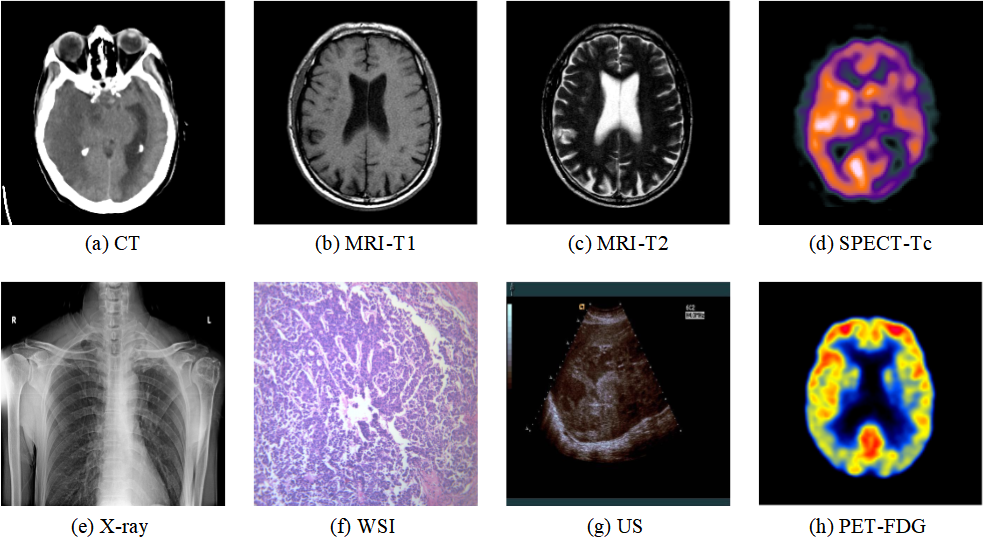
\includegraphics[width=0.9\linewidth]{figs/mul_imaging.png}
      \caption{七种不同类型的医学影像}\label{mul_imaging}
    \end{figure*}

\subsection{基于解剖结构的成像技术}
\textbf{计算机断层扫描}(CT)\cite{boyd1983cardiac}是一项以X射线成像为基础的医学影像技术,通过对人体特定部位进行X射线扫描,利用探测器接收透过人体的X射线并转换为电信号,最终生成数字化的横断面影像。其工作原理包括X射线透过人体产生的信息采集、数字影像处理和影像重建。
CT影像的构建涉及到对扫描区域的体素进行X射线吸收系数或衰减系数的测量,这些数据通过计算机处理后形成数字矩阵,再转换为灰度影像。影像的空间分辨力取决于像素大小和数目,CT影像的像素通常为1.0 × 1.0 mm或0.5 × 0.5 mm,数目可达256 × 256或512 × 512,因此,CT能够提供高度细致的解剖影像,具有较高的空间分辨力。

CT影像的特色在于其灰度表示方式,黑色代表低吸收区(低密度,如肺部含气体),白色代表高吸收区(高密度,如骨骼),而相对于传统X射线影像,CT的密度分辨力更高,能够清晰地显示组织密度差异较小的软组织结构。这使得CT在展示由软组织构成的器官(如脑、脊髓、肺等)以及病变的影像上具有突出的优势。
CT在中枢神经系统疾病的诊断上表现出色,广泛应用于颅内肿瘤、脑梗塞、脑出血、外伤性脑损伤等疾病的检测。
%螺旋CT扫描技术使其能够获得更为精细和清晰的血管重建影像,可用于CTA(CT血管成像),有望替代传统的脑血管造影
尽管CT在医学诊断领域取得了显著进展,但其使用也存在一些问题,如辐射暴露和对软组织对比度较低。随着技术的不断改进,CT仍然是一种重要的影像学工具,对于临床诊断和治疗的支持具有不可替代的作用。

\textbf{核磁共振成像}(MRI)\cite{young1984nuclear}是一种利用磁场和无线电波探测人体组织的详细横截面影像的技术。在进行磁共振成像(MRI)检查时,患者被置于一个强度高且分布均匀的静态磁场内,利用特制的无线电频率脉冲激活体内氢原子的自旋核,从而引发共振反应并捕获相应的信号。这些信号运用计算机的处理后生成高分辨率的影像,展示了人体内部的详细结构。

MRI的两种主要成像方式
%(T1、T2是用于测量电磁波的物理量,T1看结构,T2看病变)
:MRI-T1(T1反映的是纵向弛豫时间)和MRI-T2(T2反映的是横向弛豫时间),通过对比度和信号强度的不同分别对应于不同的组织特性。MRI-T1成像对脂肪组织具有较高的信号强度,呈现亮白特征,有利于显示解剖结构和脂肪组织的分布,适用于解剖结构和骨髓等的观察。相反,MRI-T2成像对水分组织有较高的信号强度,呈现亮白特征,更适用于显示水肿、炎症和软组织病变。这种高度区分不同组织的成像方式使MRI在临床上得到广泛应用,涵盖了中枢神经系统、心血管系统、关节、软组织、盆腔脏器等多个部位的病变检查。
MRI在医学影像学中的主要优势之一是对软组织的高分辨率成像。在头颅、纵隔、腹腔等实质性脏器的检查中,MRI表现出卓越的成像性能。由于人体组织成分的差异,MRI能够产生不同的信号,成为一种精准而全面的影像诊断工具。
%与传统的X线检查和核医学检查不同,MRI避免了射线辐射,因此对特定病症和人群更为安全。尽管MRI设备费用较高,对金属敏感且扫描时间较长,但在医学影像学中的不可替代作用不断凸显。

MRI技术的不断发展和创新进一步丰富了其应用领域,涵盖多种变体,如静息态磁共振成像(rsMRI)、sMRI和fMRI。每一种变体都在特定领域中展现出独特的优势。sMRI通过施加外部磁场和无线电波,激发人体组织中的氢原子核,然后测量它们在磁场中的共振信号。通过复杂的数学算法,特别是傅里叶变换,这些信号被转换成详细的影像,揭示了身体内部的精细解剖结构,为肿瘤、损伤和先天性异常等病变提供详细的解剖学信息,在神经外科和器官移植等手术前的评估中得到广泛应用。fMRI通过测量血氧水平变化,观察大脑在执行任务时的活动,提供时空分布的神经活动信息。在神经科学研究中,fMRI起到关键作用,用于研究认知功能、感觉知觉和运动执行,同时在神经精神病学和神经内科等领域用于评估神经系统疾病的功能改变。rsMRI是一项测量大脑在安静状态下血流和神经活动的成像技术。通过揭示大脑静息状态下的功能连接性,rsMRI为研究大脑的静息状态、神经网络连接性以及精神疾病、脑功能障碍等提供有益信息。这些MRI的变体在医学和研究领域中各自发挥着独特的作用,医生和研究人员可根据不同的研究和诊断需求选择适当的MRI变体,共同推动医学影像领域的不断发展,为深入理解人体生理和病理提供了丰富的信息资源,有望为未来的医学研究和诊疗提供更精准、全面的支持。

\textbf{超声成像}(US)\cite{newman1998history}是一种利用超声波对人体进行扫描的技术,它通过捕捉和分析反射回来的声波信号来构建体内器官的影像。
%其中,阵列声场延时叠加成像是超声成像领域中最传统、最简单且应用最为广泛的成像方式之一。这种方法通过对阵列的各个单元引入不同的延时,然后将它们合成为一个聚焦波束,从而实现对声场各点的清晰成像。
医学中的超声仪器涵盖了多种类型,其中B型超声是目前应用最为广泛的诊断方法。医学超声波成像是通过超声探头发出的超声波携带不同组织的回波,以构建人体内部结构的影像。
%其中A型(幅度调制型)、M型(光点扫描型)、B型(辉度调制型,即B超)、D型(基于超声多普勒原理)和C型(近似电视扫描)等是常见的。B型超声是最为广泛使用的一种成像方式,通过显示不同亮度的光点来反映接收信号的强弱,从而生成二维影像。随着技术的不断发展,还涌现出一系列新的超声技术,如灰阶显示、彩色显示、实时成像、超声全息摄影、穿透式超声成像、超声计算机断层成像、三维成像和体腔内超声成像等。
%超声诊断仪器包括A型、M型、B型、D型和彩色多普勒血流显像仪,它们各自具有独特的影像特点,其中B型超声是目前应用最为广泛的诊断方法。
医学超声波成像是通过超声探头发出的超声波携带不同组织的回波,以构建人体内部结构的影像。B模式超声影像(B超)是其中最常见的一种,其优势在于无电磁辐射、便于携带且提供实时成像。

超声诊断依赖于细致的深入观测与评估,识别不同的特征,并将这些信息整合以推断可能的病理原因。超声检查广泛应用于内脏器官的定位、测量及形态分析,同时能够帮助诊断病灶的具体范围及其性质,并提供有关腺体等组织的精确解剖影像,已在眼科、心血管以及妇产科等多个医疗领域得到普遍采用。
医生在超声检查中综合评价器官的形态、尺寸、质地、病变的声学特性、对后壁声波的影响、内部结构、位置关系及功能表现。对于不同类型的病理性影像特点,例如囊性与实质性病变、均质性与非均质性病变、钙化性与含气性病变、炎性与纤维化病变以及良性与恶性病变,医生能够通过综合观察进行诊断和鉴别诊断,为制定治疗方案提供重要参考。

\subsection{基于功能性的成像技术}
\textbf{单光子发射计算机断层成像术}(SPECT)\cite{jaszczak1980spect}是一种重要的医学成像技术,通过利用放射性同位素的$\gamma$射线,提供了对生物体内部功能和生物学过程的独特洞察。该技术基于放射性同位素的放射性衰变原理,通过测量$\gamma$光子的产生和探测,以获取有关生物体内部结构和功能的信息。
%SPECT的基本成像原理涉及患者摄入含有适当半衰期的放射性同位素药物,如锝-99m等。当这些药物到达需要成像的断层位置时,由于放射性衰变,产生$\gamma$光子。外层的$\gamma$照相机探头分布在病人周围,负责探测沿一条投影线进来的$\gamma$光子。通过闪烁体将探测到的高能$\gamma$射线转化为光信号,再通过光电倍增管将光信号转化为电信号。这些测量值代表了人体在该投影线上的放射性之和。通过多个观测角度,可以获取多个断层的平行束投影,称为平片。计算机断层成像术(CT)通过从不同角度观测,重建断层影像,将其转化为SPECT技术的重要应用。

SPECT在分辨率方面存在一些限制,如相对较低的空间分辨率和较差的时间分辨率,但其在医学影像学中的广泛应用使其成为疾病诊断和治疗方案制定的不可或缺的工具。SPECT的优势在于其提供的是功能性信息,而非仅仅是解剖结构。这对于疾病的早期诊断和治疗效果评估至关重要。如:
%心脏灌注断层显像是SPECT在心血管领域的应用的代表。它对冠心病、心肌梗死等疾病的诊断提供了支持。通过评价冠状动脉病变范围,对冠心病危险性进行分级,以及对心肌细胞活力的评估,SPECT为心血管疾病的精准诊断和治疗提供了有力工具。
在神经科学领域,局部脑血流断层显像是SPECT的一项关键应用。它对缺血性脑血管意外、癫痫致痫灶的定位等提供了高度准确的诊断。这项技术在判断脑肿瘤的血运、鉴别术后或放疗后的复发和瘢痕等方面也具有独特优势。
AD的早期诊断是SPECT在神经影像学上的又一亮点。通过对AD患者的局部脑血流进行研究,SPECT为该疾病的早期诊断提供了一致的共识。相较于传统的CT,SPECT在痴呆程度和认知状况相近的两类痴呆的鉴别上更为可靠。
%然而,SPECT的分辨率问题仍然是该技术面临的挑战之一。空间分辨率通常较低,受$\gamma$射线穿透能力和探测器灵敏度的限制。这限制了SPECT在显示小尺寸结构方面的能力。此外,时间分辨率相对较差,因为需要较长的采集时间来获取足够的数据。这使得SPECT在一些需要高时间分辨率的应用场景中受到限制。

%尽管SPECT具有一些限制,但其优势包括提供丰富的功能性信息、多模态成像、全身成像和无创性检查。它是一种非常有价值的临床工具,特别是在疾病的早期诊断和治疗方案的制定上。同时,SPECT在医学影像学中与其他技术的结合,如计算机断层成像术(CT),形成了SPECT/CT系统,为医生提供更全面的影像信息。
然而,SPECT也存在一些挑战和局限性。其中之一是辐射暴露,因为该技术需要使用放射性同位素。尽管通常在安全范围内,但这仍然是需要考虑的问题。此外,SPECT的设备和维护成本相对较高,这可能限制其在某些医疗机构的推广和应用。同时,SPECT依赖放射性同位素的摄入,这可能涉及到一些限制和患者安全的问题。
%综合而言,SPECT作为一种功能性成像技术,在医学影像学中发挥着重要作用。尽管其分辨率方面存在一些限制,但其在疾病的早期诊断、病理学分析和治疗方案制定方面提供了重要的支持。随着技术的不断发展,SPECT在医学领域的地位有望不断提升,为更准确的疾病诊断和治疗提供更多可能性。

    
\textbf{正电子发射断层成像术}(PET)\cite{raichle1983positron}作为一种核医学成像手段,它依赖于正电子在湮灭过程中释放的辐射光子。在这个过程中,回旋加速器将带电粒子加速,并轰击特定的靶核,进而生成正电子放射性核素。通过精心设计的探测器阵列和高效的符合电路,PET能够检测到这些湮灭光子对,并据此绘制出体内正电子核素的截面分布图。这种影像能够清晰地展示病变的位置、形状、大小,以及相关的代谢功能,为医生提供宝贵的诊断信息。
%尽管PET存在辐射剂量较大和设备成本高的缺点,但其独特优势在于提供高分辨率的功能性信息,广泛应用于肿瘤学、心血管学等领域,为疾病的早期诊断和治疗效果评估提供重要支持。

在肿瘤学中,PET成像被广泛用于癌症的早期诊断、分期、治疗效果评估和复发监测。18F-FDG(2-氟-18-氟-2-脱氧-D-葡萄糖)是一种常用的显像剂,通过显示异常的葡萄糖代谢水平,PET可以精准定位和描绘肿瘤。在实际应用中,患者接受18F-FDG药物注射后,PET扫描仪通过探测正电子湮灭事件获取体内放射性核素分布情况。影像分析利用标准化摄取值(SUV)等定量测量,对病变的代谢活性进行评估,为肿瘤生物学特性、治疗反应和复发监测提供关键信息。

%在心血管学中,PET可评估心肌的代谢和灌注情况,用于诊断和监测冠心病、心肌梗死等疾病。正电子放射性核素的注射提供心肌代谢信息,例如18F-FDG PET用于评估心肌葡萄糖代谢。此外,PET与CT结合可提供更全面的心血管影像信息,为精准诊断和治疗规划提供支持。

在神经学领域,18F-FDG PET在AD早期诊断中取得显著进展。通过评估脑部葡萄糖代谢情况,PET揭示患者大脑功能异常,为AD的诊断和病程监测提供关键信息。 PET的高分辨率和功能性信息使其在医学中的应用不断拓展,为多领域的疾病管理提供了更全面、精准的影像学支持。

\subsection{基于其他类型的成像技术}
\textbf{X射线}(X-ray)\cite{warren1990x}是一种电磁辐射,在医学影像学中,X射线被广泛用于探测和成像,广泛用于识别骨骼问题、胸部及腹部疾病,包括肺部与肠道堵塞等状况。X射线成像主要依赖于光电效应,通过测量透射或散射的X射线来获取关于人体内部结构的信息。
%X射线的分辨率取决于成像设备的性能,现代X射线设备通常能够提供较高的分辨率,能够清晰地显示细小的解剖结构。X射线的成像机制是通过穿透物体并被探测器接收,形成影像。这使得医生能够检查骨骼、器官和其他组织的内部结构,帮助做出准确的诊断。然而,对于柔软组织和微小病变的检测,X射线的分辨率相对较低,有时需要进一步的影像检查或其他影像技术的辅助。

%X射线成像的原理是通过X射线的吸收和散射来区分不同组织的密度和构造。当X射线经过人体时,不同组织对X射线的吸收能力不同,因此在胶片或数字探测器上形成不同的灰度影像。这些影像可以由医生进行解读,从而进行疾病的诊断和评估。
X射线成像的优点之一是其广泛的应用范围和相对较低的成本。X射线设备相对便宜且易于使用,使得它在许多医疗机构中得到了广泛的普及。此外,X射线成像速度快,可以提供即时的影像结果,对急诊情况和危重患者的救治具有重要意义。
然而,X射线成像也存在一些缺点和风险。首先,X射线是一种电离辐射,长期频繁暴露可能对人体产生辐射损伤的风险,特别是对于儿童和孕妇。其次,X射线成像对柔软组织的分辨率较低,不适合检测早期病变或微小的异常。

%综上所述,X射线成像具有快速、广泛应用和相对低成本的优点,但也存在辐射风险和对柔软组织分辨能力有限的缺点。在实际应用中,医生会根据患者的具体情况和病情选择合适的影像技术来进行诊断和评估。

\textbf{显微镜}\cite{haider1998electron}作为一种基于凸透镜成像的仪器,在医学中发挥着广泛的作用。通过物镜和目镜的双重放大过程,显微镜能够将微小物体放大到人眼可分辨的尺寸,为医学研究提供了重要的支持。
%其主要组成部分包括目镜、物镜、载物台和反光镜,其中物镜的焦距小于目镜,而反光镜用于反射光线,照亮被观察的物体。
在医学领域,显微镜的应用涉及组织学、细胞学和病理学等多个方面。通过观察组织切片(whole slide image,WSI),显微镜可以提供高分辨率的影像,帮助医生深入了解微观结构,从而支持准确的疾病诊断和治疗方案的制定。

特别是在癌症研究和诊断领域,显微成像技术发挥着至关重要的作用。如:
%显微成像可用于深入研究癌症组织的结构和形态学特征。通过对组织切片的显微观察,医生能够详细了解癌细胞的外观、大小、核形态等信息,有助于明确肿瘤类型。另外,
显微镜下的成像可用于对癌症病理学进行详细分析,包括观察组织的完整性、细胞浸润深度以及细胞变化的程度。这些信息对于判断肿瘤的恶性程度至关重要。尽管显微镜具有高分辨率、实时观察和非侵入性等优点,但也存在一些挑战,如有限的穿透深度、专业训练要求和较高的设备成本。
近年来,随着技术的不断创新,显微成像在医学领域的应用前景将继续扩展。新兴技术如活体显微镜技术使得在活体动物或人体上进行实时显微观察成为可能,为研究疾病的生长过程、细胞动态和治疗效果提供了更为深入的理解。
%总体而言,显微成像技术在医学研究中发挥着不可替代的作用,为深入了解疾病机制和制定更精准的治疗方案提供了强大的工具。
   \begin{table*}[htbp]
      \centering
      \small
          \caption{不同的医学影像成像机制、分辨率及优缺点对比}\label{imaging_contrast}     
            \begin{tabular}{cccm{2.7cm}<{\centering}m{2.7cm}<{\centering}}
            \hline
            \textbf{\textit{Imaging}} &成像机制 &分辨率 &优势 &局限性  \\ \hline
            \textbf{X-ray} &X射线 &[0.1mm,~1mm]  &成像速度快、价格低、广泛应用  &X射线有害、软组织成像效果差  \\ \\
            \textbf{CT}	&X射线  &[0.5mm,~2mm]  &成像速度快、价格低、骨组织敏感  &X射线有害、软组织成像效果差、有伪影  \\ \\
            \textbf{MRI} &磁共振  &[0.5mm,~1.7mm]  &软组织成像效果好、无骨伪影  &硬组织成像效果差、时间较长  \\ \\
            \textbf{US}  &超声波  &[1.5mm,~2mm]  &成本低、无损耗、使用方便  &分辨率较低、无法穿透骨骼、空气、存在折射效应  \\ \\
            \textbf{SPECT} &$\gamma$射线  &[3.5mm,~10mm]  &对比度高、提供功能性信息、价格较低  &分辨率较低、速度慢、放射性同位素的摄入  \\ \\
            \textbf{PET} &核  &[4mm,~6mm]  &高分辨率、提供功能性信息  &放射性同位素的摄入、成本较高  \\ \\
            \textbf{WSI} &凸透镜  &[200nm,~0.2$\mu$m]  &高分辨率、实时观察、非侵入性  &有限穿透深度、需要专业训练、成本较高  \\  \hline
            \end{tabular} 
    \end{table*}


不同的成像机制可以获得不同的医学影像,并根据不同的特性应用于不同的疾病诊断中,各自的特性比较如表\ref{imaging_contrast}所示,表中的分辨率通常在给出的参考范围内,具体值取决于设备的类型和扫描参数等使用的条件。X-ray主要用于颅骨成像,对于骨折和骨质疾病的检测具有优势。CT提供高分辨率的骨髓和软组织影像,对脑肿瘤的大小和位置具有关键意义。MRI适用于探测脑部软组织病变,如脑肿瘤、AD等。US在产前检查和婴儿脑部检查方面有优势。SPECT在AD早期诊断方面有帮助,而PET在脑肿瘤代谢活性和AD脑代谢方面表现出色。显微成像对神经系统疾病的基础研究和理解细胞水平变化至关重要。在实际应用中,这些成像技术的综合运用可以更全面地观察和诊断疾病。
%例如,X射线和CT适用于颅骨骨折检测,MRI用于详细结构描绘脑肿瘤,SPECT和PET提供关于脑功能和代谢的信息,显微成像则助力深入理解神经系统疾病的微观变化。

在医学影像领域,倘若有一台能够扫描多模态的医学影像数据的机器会极大地提高诊断效率和准确性。然而,由于成本和设备更新的限制,在国内医疗环境中,许多医院只拥有特定类型的扫描仪,其产生的影像局限于该仪器的特性。这就迫使医生必须根据需要使用不同的设备,增加了工作的复杂性。若有一种简便且高效的算法,能够将来自不同设备的影像进行融合,将为医学影像的多模态融合提供一种经济高效的解决方案。
因此,开发出能够实现多模态融合的算法,不仅能够在医学影像的全面性诊断上大显身手,同时也能为医院节省设备购置成本和提高工作效率。这种简单而实用的技术创新,无疑将为医学领域带来福音。



\section{智能影像组学技术的理论基础}


\subsection{医学影像组学关键技术介绍}
%随着人工智能技术的迅猛发展,涌现出许多分类模型,主要分为基于传统的机器学习(Machine Learning,ML)方法和基于深度学习(Deep Learning,DL)方法两大类别。这些分类模型在医学领域的应用正不断扩展和深化,涵盖了诸如肿瘤检测、疾病诊断、影像分割等多个方面。它们不仅提高了医学影像分析的效率,同时为医疗诊断带来了更准确的结果。在医学科研和临床实践中,这些模型的不断进步为提升医学影像技术水平和改善患者医疗体验贡献了重要力量。
医学影像组学是一个交叉学科领域,它结合了医学影像学、生物信息学、计算机科学和数据科学等多个学科的知识和技术。在过去,医学影像组学的分析往往依赖于传统的手工设计特征,即研究者根据以往的经验和知识来选择和定义特征。在智能辅助诊断方面,最初主要依赖于基于机器学习的方法,这些方法通常需要人工设计特征,即研究者需要根据专业知识来选择或构造用于模型训练的特征。然而,近年来深度学习技术的兴起和发展,使得医学影像组学能够通过神经网络来自动学习和提取特征,这一变革减少了对专家知识的依赖,显著提高了特征提取的效率和准确性。

\subsubsection{基于传统的机器学习方法}
基于传统的ML方法,如支持向量机(SVM)、决策树、随机森林等,以其稳定性和可解释性在医学影像分类任务中取得了显著的成果。%这些方法通过提取手工设计的特征,对医学影像进行分类和识别,为医学诊断提供了一种可靠的解决方案。
本章将多种常见的ML方法进行比较,见表\ref{ML_contrast},并详细分析经典的SVM分类器。

   \begin{table*}[htbp]
      \centering
          \caption{常见的基于传统的机器学习方法对比}\label{ML_contrast}     
            \begin{tabular}{m{3.2cm}<{\centering}m{4.2cm}<{\centering}m{4.2cm}<{\centering}}
            \hline
            \textbf{\textit{ML方法}}  &优势 &局限性  \\ \hline
            \textbf{支持向量机}  &SVM模型只与支持向量有关、高维数据中只需少量的样本、节省了内存,鲁棒性强  &非线性SVM需要进行核函数映射、计算开销较大  \\ \\
            \textbf{贝叶斯}	  &实现简单、收敛速度快、聚类效果较优、无参数训练模型  &k需要人为设定、只能得到局部最优解、抗干扰差、非凸数据集难以收敛  \\ \\
            \textbf{决策树}  &对数据要求度低、速度快、准确性高、适合高维数据  &在训练数据上比较耗时、在面对复杂的高维数据时容易过拟合  \\ \\
            \textbf{随机森林}    &实现简单、准确性较高、适合高维数据  &整组数据的决策树上容易过拟合、训练时间较长  \\ \\
            \textbf{逻辑回归} &计算速度快、适合二分类、内存占用小、模型可解释性好  &不能解决非线性问题、很难处理数据不平衡的问题、准确率不高  \\ \\ 
            \textbf{K-最近邻} &实现简单、可直接在测试数据上查找最近的邻居来进行分类 &依赖于距离度量、计算成本高、不适用于高维稀疏数据
             \\  \hline
            \end{tabular} 
    \end{table*}
    
   \begin{figure*}[htbp]
      \centering  
      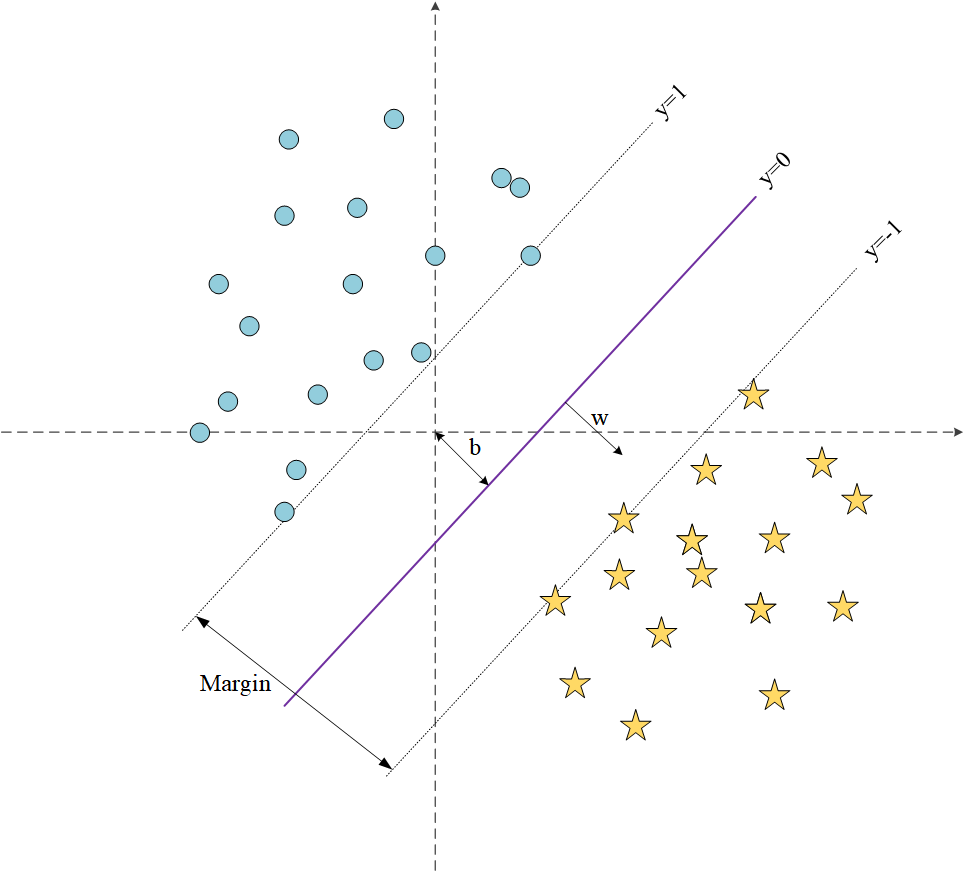
\includegraphics[width=0.9\linewidth]{figs/svm.png}
      \caption{线性可分SVM}\label{svm}
    \end{figure*}
    
在二分类模型中,支持向量机(SVM)是一种广泛应用的方法。其核心分类思想是寻找一个能够将样本分割并具有最大间隔的超平面。这里的“间隔最大”指的是确保超平面与其最近的样本点的距离最大。通过最大化间隔,SVM能够提高分类预测的可信度。如图\ref{svm},中间的实线即为所求的最优超平面,虚线边界上的点被定义为支持向量。最优超平面到两侧虚线边界的距离是相同的,这个距离称为几何间隔,Margin即为两倍的几何间隔,其计算为$2/\|\mathbf{w}||$。y是分类面,其计算为$\text{wx+b}$。线性可分SVM可归为凸二次规划问题,针对该类问题可以考虑用Lagrange乘子法进行求解,目标函数为公式(\ref{SVMst})。
\begin{equation}\label{SVMst}
\begin{aligned}\min\frac{1}{2}\|W\|^2\\\\s.t.\quad y_i\left(W^Tx_i+b\right)\geq\pm1\end{aligned}
\end{equation}

线性可分SVM在面对非线性可分的样本集时显然存在局限性。为了解决这一问题,SVM采用了核函数$\phi(x)$的方法,典型的核函数包括RBF(径向基函数),poly(多项式核函数),linear(线性核函数),sigmoid等。SVM使用这些核方法把数据映射到高维,以便更好地分离。具体而言,非线性可分SVM的模型可以表示为式(\ref{svm2}):
\begin{equation}\label{svm2}
f(x)=W^{T}\phi(x)+b
\end{equation}

其中,$\phi(x)$表示样本在高维空间中的映射,$W$是对应的权重向量,$b$是偏置项。通过这样的映射,原本在低维空间中无法线性分隔的样本,在高维空间中找到了一个线性超平面,从而完成了分类任务。这种非线性可分SVM的处理方式为算法赋予了更大的灵活性,使其能够更好地适应实际场景中存在复杂结构和非线性关系的数据。
%在医学领域,特别是医学影像分类与预测任务中,这种能够处理非线性关系的SVM模型为提高准确性和适用性提供了有力的工具,有助于更精准地识别和预测医学影像中的复杂模式。在多分类问题中,支持向量机(SVM)采用直接法和间接法两种构建策略。直接法通过修改目标函数解决多个超平面参数的最优化问题,适用于小型数据集但计算复杂度较高。间接法基于多个二分类器构建多分类器,有“一对一”和“一对其余”两种实现方式,前者需要设计 $k(k-1)/2$个分类器,后者则设计K个分类器。在实际应用中,选择适当的构建策略需考虑数据集规模、计算资源和对模型解释性的需求,这对于获得更好的性能至关重要。

SVM作为一个多才多艺的分类器,不仅在ML领域取得了成功,而且在医学影像处理中表现出色,为医学领域的疾病诊断和预测提供了强大的支持。其能够同时应对线性和非线性的分类任务,为医学影像的自动化分析和医生的决策提供了可靠的辅助。
%尽管SVM在医学影像处理中具有许多优点,包括高准确性和泛化能力,但在处理大规模数据、调整核函数参数以及对噪声和异常值的敏感性等方面仍然存在一些挑战。在实际应用中,需要仔细权衡其优势和缺陷,并结合具体问题的特点选择适当的算法。

\subsubsection{基于前沿的深度学习方法}
基于DL方法的发展更是推动了医学影像处理的前沿。卷积神经网络(CNN)和循环神经网络(RNN)等深度学习架构通过学习影像的高级特征表达,使得模型能够自动从数据中学习到更抽象、更复杂的表示,从而在医学影像分类中取得了卓越的性能。DL方法的主要优势在于其端到端的学习能力,对于复杂和大规模数据集的处理能力更为突出。

   \begin{figure*}[htbp]
      \centering  
      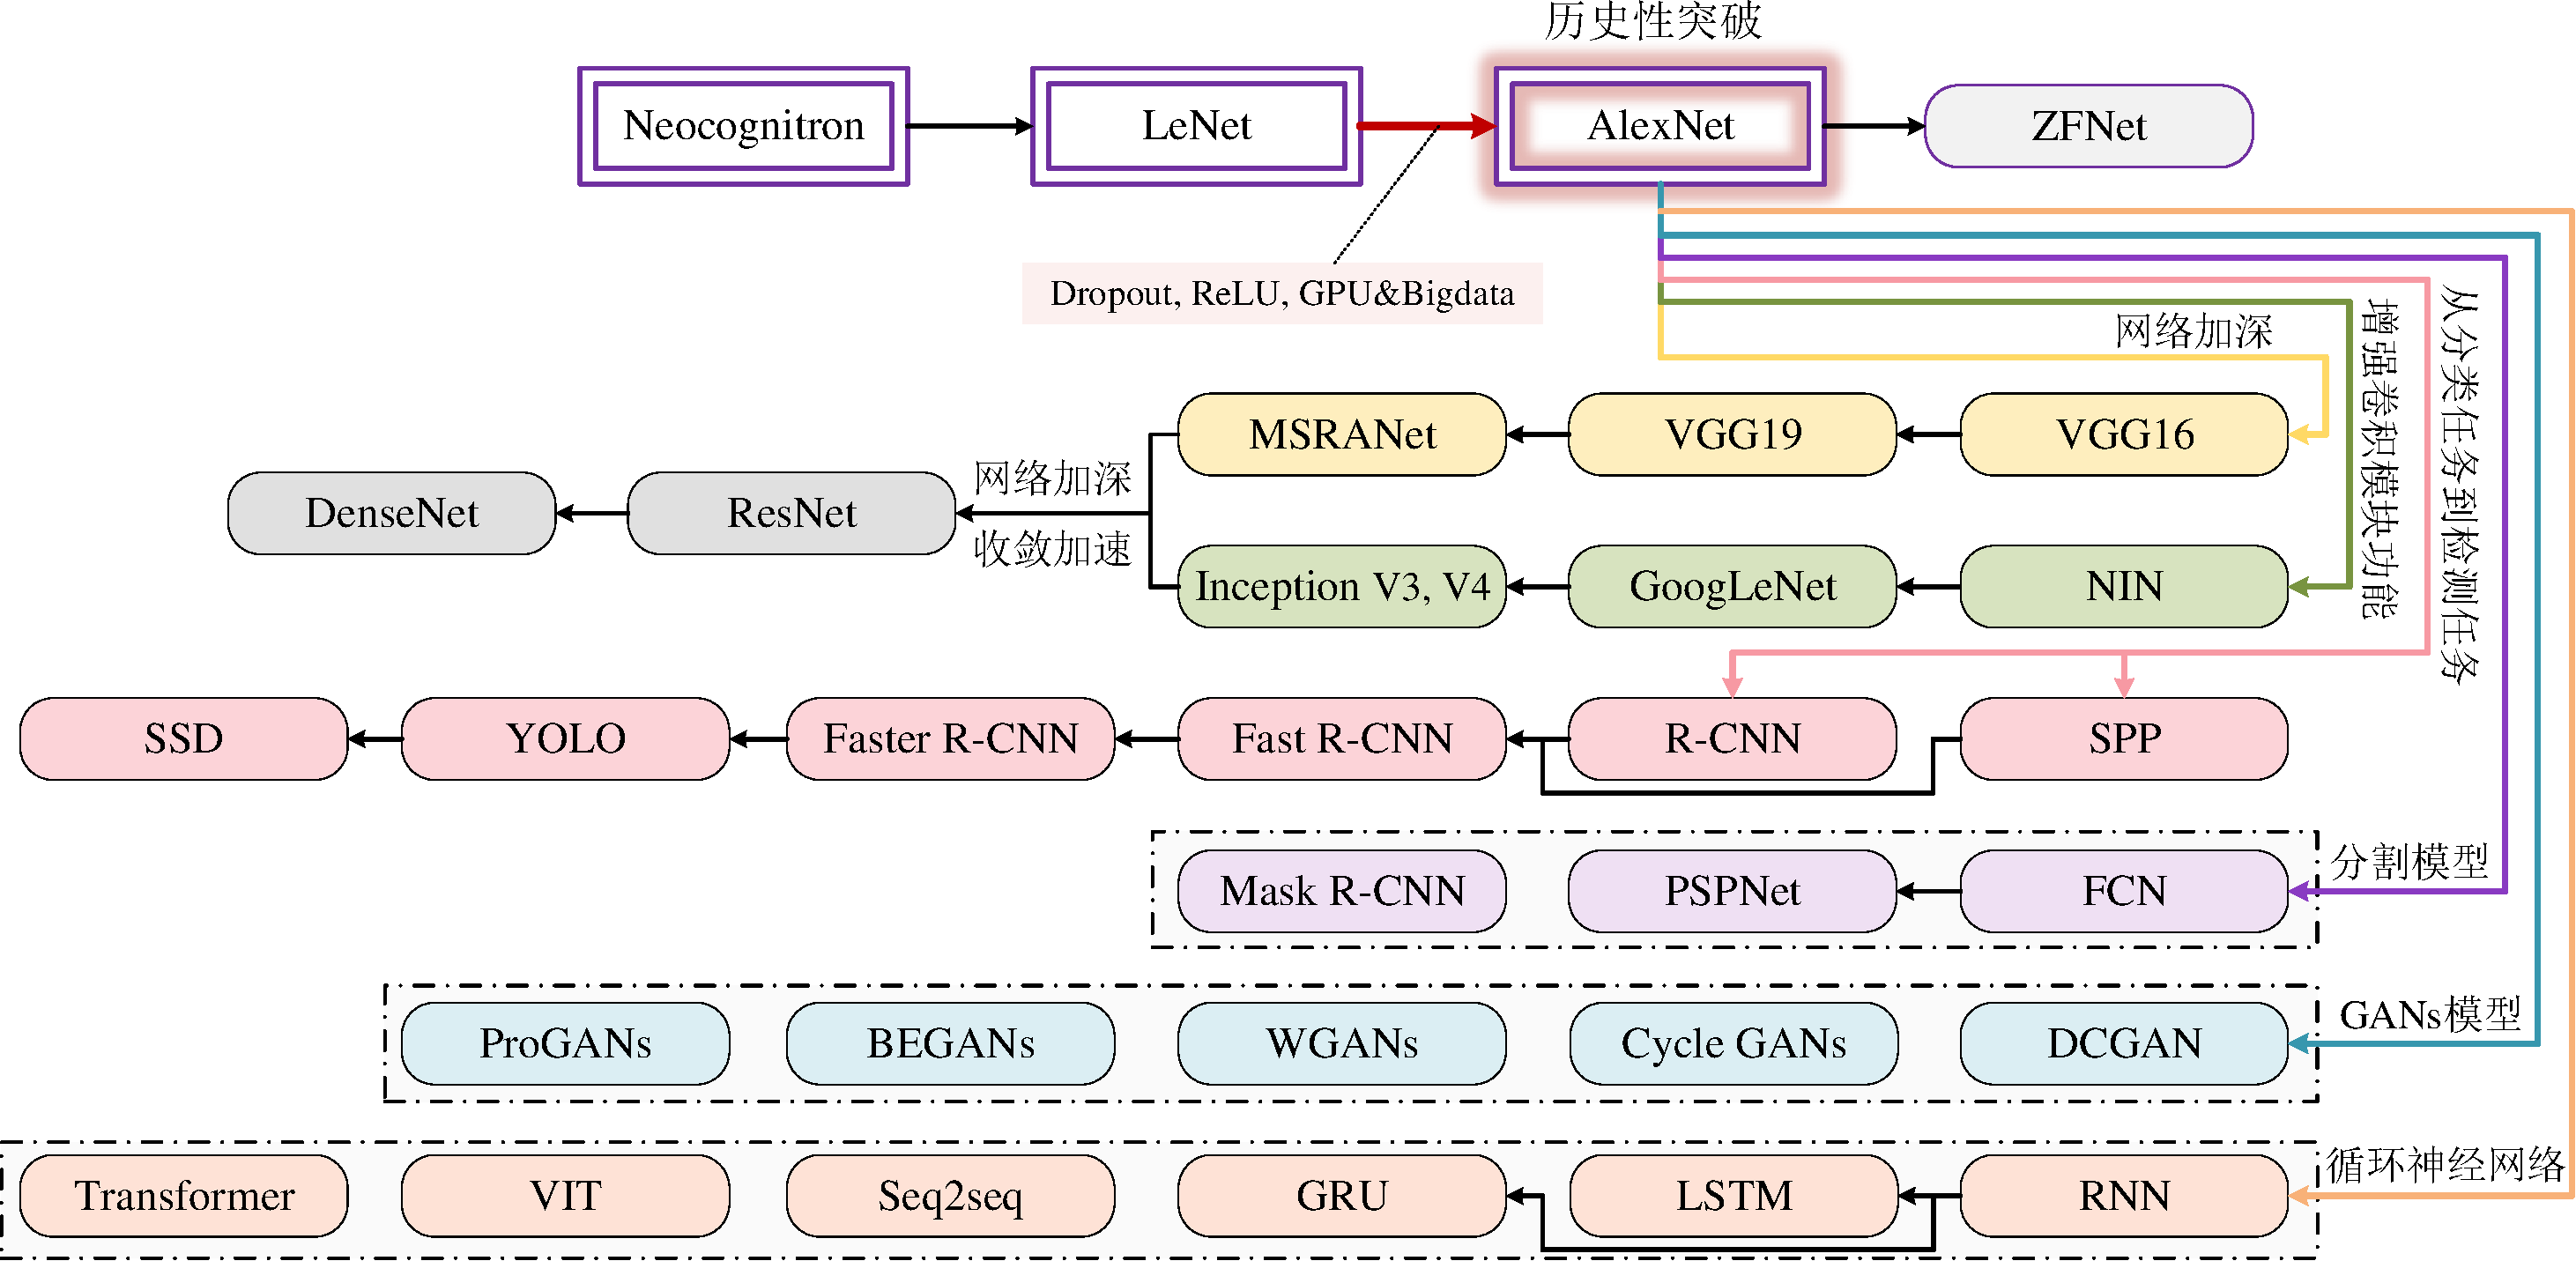
\includegraphics[width=0.9\linewidth]{figs/CNNdevelopment.pdf}
      \caption{深度神经网络发展脉络}\label{CNNdevelopment}
    \end{figure*}
    
CNN代表了DL领域的重要里程碑,其模拟了生物神经元结构的并行计算方式,能够在分类任务中自动学习和提取数据中的抽象特征,从而无需依赖手工设计的特征。CNN相对于传统机器学习方法在影像融合、分类、预测等任务中具有显著优势。其核心技术包括卷积、激活、批归一化、池化和全连接。
在影像分类领域,CNN通过卷积操作实现对输入影像的特征提取,利用局部感知和权值共享机制捕捉影像的局部特征,使得模型能够更好地适应数据的复杂结构。激活函数引入非线性,如Sigmoid、Tanh、Softmax和ReLU,赋予模型对复杂关系的学习能力。批归一化在神经网络的中间层中规范输入,加速训练过程,提高模型的稳定性。池化操作通过降采样减小特征图的尺寸,有助于保留重要信息并降低计算复杂度。全连接层整合局部特征,并将其映射到样本标签空间,完成最终分类。

    
CNN在实际应用中展现出卓越的性能,尤其在计算机视觉领域,为处理庞大而复杂的数据集提供了高效而强大的解决方案。图\ref{CNNdevelopment}为CNN的大致发展脉络。其中,LeNet\cite{lecun1998gradient}作为CNN的经典之作,为DL领域的发展奠定了坚实基础,成为影像分类和识别领域的开创性工作。AlexNet\cite{krizhevsky2012imagenet}在某种程度上继承并发展了LeNet的思想,并且引入了一些新的技术,如在CNN中广泛使用了ReLU激活函数,使用了Dropout技术防止过拟合,并采用了GPU加速训练过程。AlexNet的模型结构如图\ref{Alexnet}所示,它在2012年的ImageNet大规模视觉挑战赛
%(ImageNet Large Scale Visual Recognition Competition,ILSVRC)
中取得了冠军,其不仅在性能上大幅超越了当时的其他方法,而且其成功也证明了DL在处理大规模视觉识别任务中的巨大潜力,极大地促进了DL在各个领域的应用和发展。 

AlexNet等CNN网络模型在医学领域的应用为医学影像分析、疾病诊断和个性化医疗等方面带来了巨大的进步,推动了医学影像组学分析技术的发展,为医学诊断和治疗提供了全新的思路和工具。
一些经典的网络模型在医学领域取得了显著的成果,如FCN\cite{long2015fully}作为一种专门用于影像分割的模型,特别适用于医学影像的病灶分割等任务。
U-Net\cite{ronneberger2015u}是一种用于生物医学影像分割的经典网络模型,结构简单,同时在分割任务中表现出色。因此,医学领域广泛采纳并应用了这项技术。
总的来说,CNN网络模型在医学领域的应用为医疗诊断、疾病预测和治疗方案的制定带来了更多的可能性和机会,有助于提高医疗保健的水平和效率。

 \if 0
   \begin{figure*}[htbp]
      \centering  
      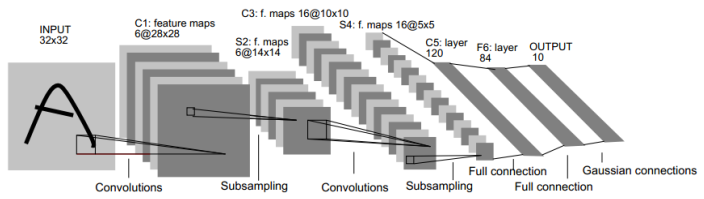
\includegraphics[width=0.9\linewidth]{figs/Lenet.png}
      \caption{Lenet网络结构}\label{Lenet}
    \end{figure*}
  \fi

   \begin{figure*}[htbp]
      \centering  
      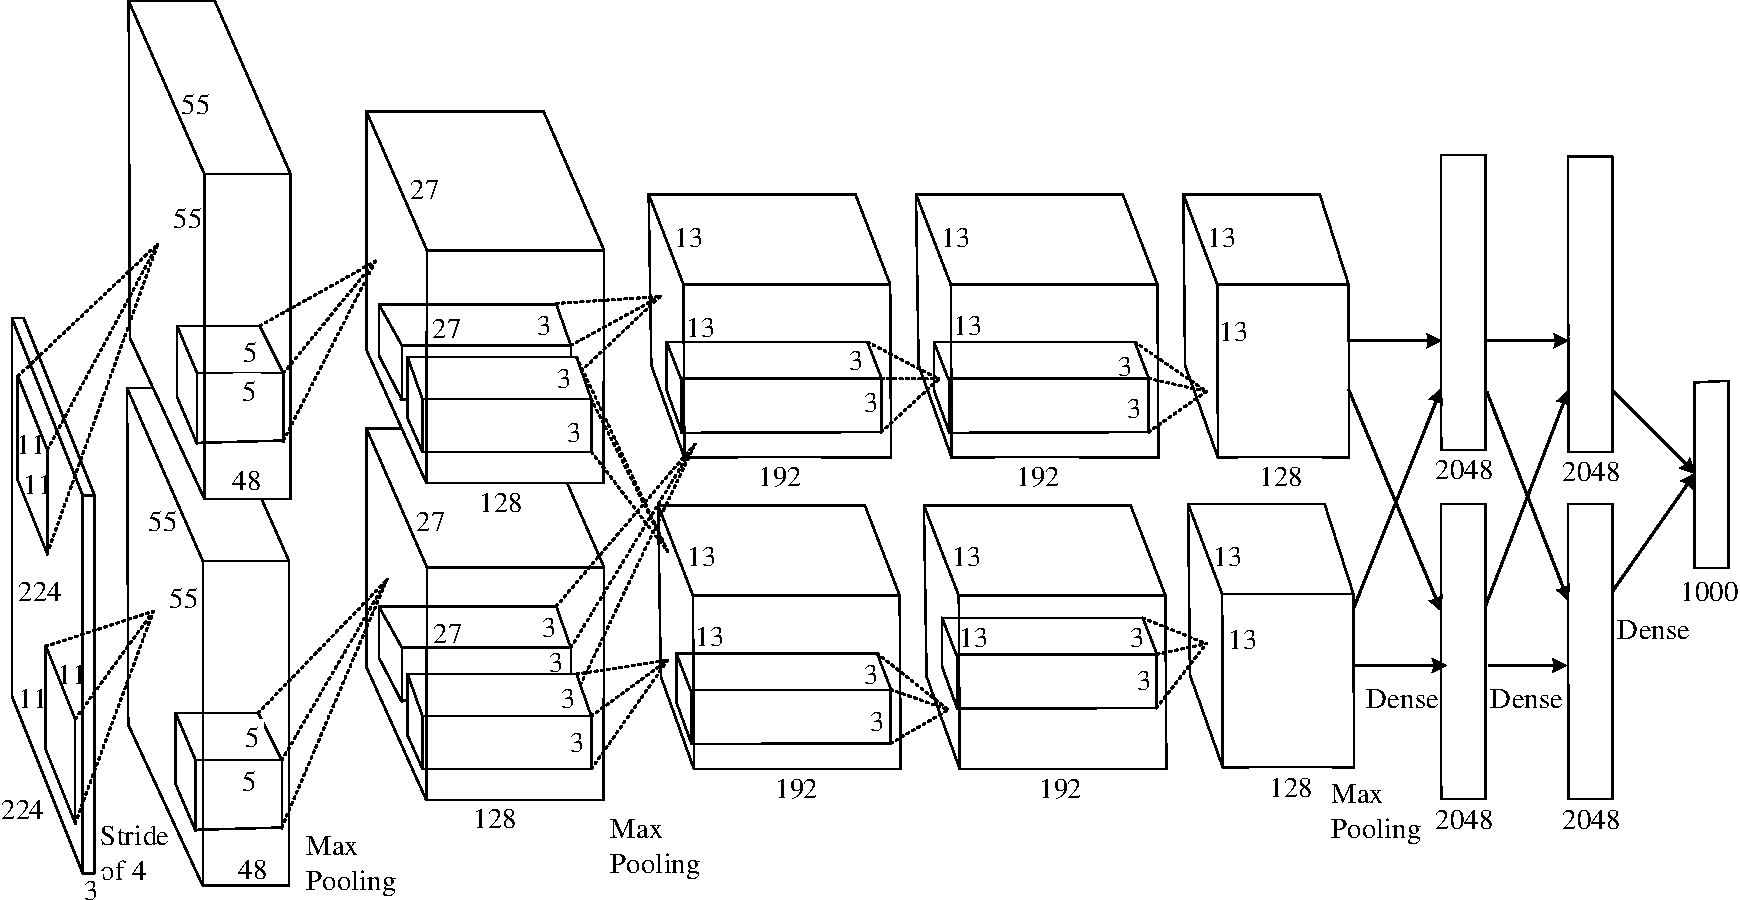
\includegraphics[width=0.9\linewidth]{figs/alexnet.pdf}
      \caption{AlexNet\cite{krizhevsky2012imagenet}网络结构}\label{Alexnet}
    \end{figure*}
%LeNet是LeCun等科学家于1998年提出的CNN模型,最初应用于手写数字和英文字母的识别任务\cite{lecun1998gradient}。该模型结构如图\ref{Lenet}所示,其包括7个层次,其中包括3个卷积层、2个池化层和2个全连接层。LeNet的输入影像尺寸为32x32,虽然规模较小,但其各个模块的设计十分完备,为后续深度学习模型的发展奠定了基础,被认为是CNN的基石之一。LeNet的结构设计反映了卷积神经网络的基本原理,通过卷积和池化层逐渐提取影像的层次化特征,最终通过全连接层进行分类。LeNet的成功证明了CNN在处理视觉任务上的有效性,为后续深度学习研究和应用的发展打下了坚实基础。


%医学领域对影像技术的需求不断增长,这两种类型的分类模型都在不同的场景中展现了强大的潜力。传统方法在数据较为有限或需要解释性强的情况下具备优势,而深度学习方法则在处理大规模数据和复杂特征提取方面取得了显著的成就。因此,这两者的结合和并行应用成为医学影像分类领域的一个前沿趋势,为更准确、高效的医学诊断提供了新的可能性。

\subsection{影像组学技术的信息融合策略}
信息融合涵盖了不同医学影像之间的融合(多模态融合),例如CT与SPECT的融合、CT与MRI的融合、MRI与SPECT的融合甚至是三种影像的融合。同时也包括影像和其他异构数据之间的融合(跨模态融合),如临床指标与医学影像之间的融合。作为一种关键的影像处理策略,尤其在多模态医学影像领域,影像信息融合通过综合多种影像信息并采取相应的融合策略,可以显著提高影像的质量和信息量。常见的融合方法主要分为三种:像素级、特征级以及决策级融合。

这三种融合方法在多模态影像融合、AD分类和PD预测的研究中备受关注。在多模态影像融合方面,这些方法为整合不同成像模态提供了高效手段,有助于充分利用各种影像信息,提高影像的全面性和信息量。在AD分类和PD疾病预测领域,融合方法的应用为更准确、可靠的疾病诊断和预测提供了新的思路和工具。通过综合不同模态的信息,可以更全面地了解患者的病理状态,为个性化治疗和康复提供更为精准的支持。这些研究不仅推动了医学影像处理技术的进步,也在提升脑部疾病的辅助诊断水平方面取得了显著的研究成果。

\subsubsection{基于像素级的技术方案}
像素级融合技术涉及在影像处理的基础层面上,对原始影像数据的像素点进行直接操作和整合,形成新的像素值,进而生成融合影像。这一方法在影像信息融合中起到重要作用,特别是在像PET和MRI影像的融合中。像素级融合技术能够有效地结合不同影像源的信息,从而增强影像细节,这有助于提升疾病诊断的准确性。将PET-MRI影像对采取像素级融合可以充分发挥PET在发现受试者脑部葡萄糖代谢变化方面的优势,尤其在AD患者中,PET可揭示脑部葡萄糖摄取降低、导致脑萎缩的情况。虽然PET影像本身的细微解剖结构分辨率不甚理想,但通过与MRI技术的联合应用,能够显著提升影像的整体清晰度和细节丰富度。二者的融合可以克服各自的局限性,为痴呆患者的病程分析提供更全面的信息。通过综合PET和MRI的数据,可以更准确地评估AD患者的病变程度,为医生提供更为精确的诊断和治疗决策支持。因此,像素级影像融合在神经学领域中的应用有望在脑部疾病的诊断和治疗方面发挥关键作用。

   \begin{figure*}[htbp]
      \centering  
      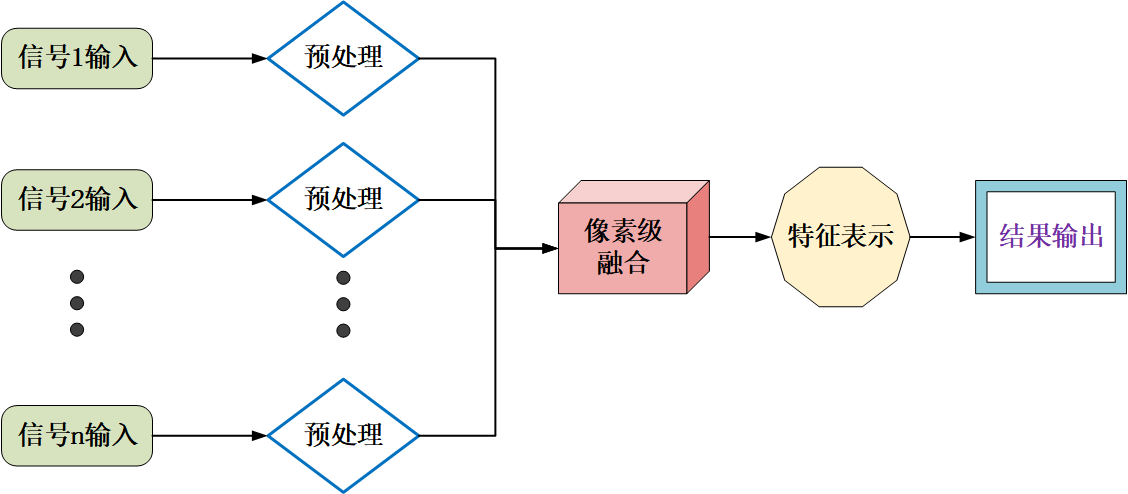
\includegraphics[width=0.9\linewidth]{figs/pixelFusion.png}
      \caption{像素级信息融合机制}\label{pixelFusion}
    \end{figure*}
    
如图\ref{pixelFusion}所示,像素级影像融合通过各类不同和类型的输入数据执行预处理操作,并采用特定的计算策略计算新的像素点数值,最终生成融合影像。这种融合策略有效地整合了来自不同来源的信息,引入更加细致的信息,并强化了影像的相关特征,具备高度的精度。像素层面的影像融合的独特之处在于能够最大限度地保留源影像中的内容,使得融合后的影像内容和细节都得到了增强。该方法有助于突显潜在目标,判断和识别潜在目标的像素点,为影像的理解和分析处理提供有力支持。

尽管像素级影像信息融合具有显著的优势,但也面临一些局限性。首先,由于像素级融合涉及大量数据的计算处理,可能导致较长的处理时间,实现实时处理与显示是一项挑战;其次,由于数据量庞大,在通信传输过程中,此类信息更易受到噪声影响。此外,如果参与融合的源影像没有经过精准配准处理,则融合后的影像可能出现模糊不清、目标定位不准确以及细节信息失真的问题。

\subsubsection{基于特征级的技术方案}
特征级影像融合通过先对不同模态原始数据进行预处理,接着运用各类模型提取各自特有的信息特征,再依据特定融合规则,将这些各异模态数据的特征有效整合起来,如图\ref{featureFusion}所示。
%以CT和MRI两种不同模态的数据为例,该融合方法首先对这两种不同模态的数据进行预处理,然后利用不同或相同的网络模型提取CT或MRI影像的特征,最后利用融合后的特征进行输出。特征级影像融合的独特之处在于能够包含不同模态影像的特征之间的相关性和交互信息,从而融合更多信息,获取更具判别力的特征表示。这种融合方法有助于综合不同模态的信息,提高对复杂目标的识别能力。
通过深度学习等技术,特征层面的影像融合技术可以自动学习并提取不同模态的有重要信息的特征,从而更好地揭示目标的多方面信息。这对于医学影像处理领域尤为关键,例如在神经影像学中,结合CT和MRI的特征级融合有助于更全面地理解脑部结构和病变。

   \begin{figure*}[htbp]
      \centering  
      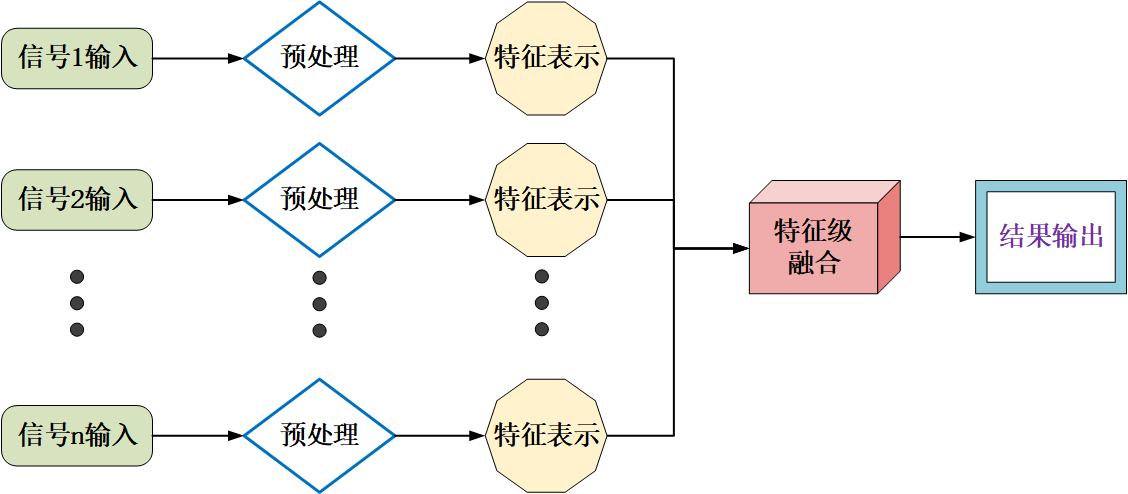
\includegraphics[width=0.9\linewidth]{figs/featureFusion.png}
      \caption{特征级信息融合机制}\label{featureFusion}
    \end{figure*}

从源影像中提取特征通常指的是识别和量化影像中的关键信息,这既包括整个影像的全局特征,也包括特定区域的局部特征(如感兴趣区域,即ROI)。例如,在医学成像领域,MRI和CT影像的特征提取旨在识别出有助于诊断的关键信息,并将这些信息进行分析和处理,以便用于后续的影像融合。通过这种方法,可以从MRI和CT影像中提取出有用的特征,然后将这些特征结合起来,形成一个更为全面的特征表示。这种特征级的影像融合方法能够有效地减少数据的冗余,提高信息的密度,从而在分类和其他影像处理任务中达到更高的准确度。相比于直接在像素级别进行融合,特征融合能够显著降低所需的计算资源和存储空间,因为它只关注影像中的重要信息,而不是每一个单独的像素。同时,特征级融合的计算速度较快,虽然对影像匹配精确度的要求相对较低。这种方法为在医学影像处理领域提供了更高效的影像信息融合策略。相比于其他方法,特征级影像融合在内存和时间上的需求较低,因此,其具有更迅速的计算效能,并能够有效提升影像处理的实时响应能力。但也可能损失部分细节性特征。

   \begin{figure*}[htbp]
      \centering  
      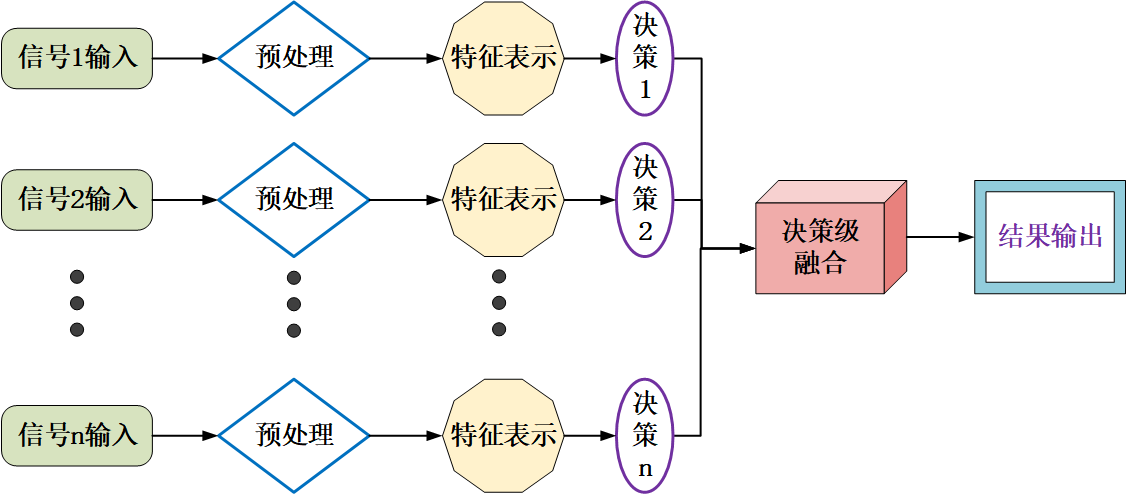
\includegraphics[width=0.9\linewidth]{figs/decisionFusion.png}
      \caption{决策级信息融合机制}\label{decisionFusion}
    \end{figure*}
\subsubsection{基于决策级的技术方案}
决策级影像融合技术被视为一种高层次的认知整合策略,它代表了影像融合技术中最复杂与最抽象的手段。此方法先将每幅影像依据各自的特征信息进行独立识别与分类处理,然后结合每个源影像的决策结果,按照一定的规则和置信度权重,如采用贝叶斯推理或是集合决策机制等,对这些决策结果进行综合集成,从而得出最优的整体判断。以SPECT和CT影像为例,在这一层级上,首先分别对两种不同模态的数据完成独立的诊断决策,随后遵循特定准则,将这两种影像的决策输出相结合,目的是为了实现整体最佳的诊断效果,进而准确区分AD病患的不同严重程度,该策略的实现如图\ref{decisionFusion}所示。

这种决策级影像融合方法在医学影像领域具有重要意义。通过将多个模态的独立决策结果合并,可以得到更全面、准确的诊断信息,提高对疾病状态的认知。例如,在AD的诊断中,结合SPECT和CT影像的决策结果,可以更全面地评估患者的脑部结构和功能,有助于提高对疾病的早期诊断和分级。这种影像融合方法的优势在于能够综合不同模态影像的信息,克服单一模态的局限性,为更准确的医学影像诊断提供支持。


决策层面的影像融合技术位于影像融合方法的顶层,它以认知理论为核心,针对具体问题需求实施深层次、有目的性的信息整合。该融合技术具有数据处理要求低、抗扰动稳定性强等优势。然而,与影像的像素级或特征级的策略相比,决策级影像融合存在明显的缺点。其关键挑战在于对前序步骤输出结果的高度依赖性,且对于影像集成的要求更为复杂。在影像集成的决策层,不仅要对每幅影像独立作出判断,而且还必须针对合并前的多项复杂预处理操作作出决策,这样的处理使得决策级融合的过程变得更加精细和复杂。

%在临床医学诊断中,成像参数、病人体位以及成像设备的差异可能导致成像质量受到噪声的影响,甚至引起几何畸变。为提高成像质量,预处理技术如影像去噪、影像配准和消除畸变等被广泛应用。这些方法有助于规范化影像,消除可能影响医学诊断准确性的因素。
%特征表示是对原始数据进行表达的过程,包括特征提取和特征选择。其目的是提升对数据的表达能力。目前,特征工程和表示学习是特征表示的两个主要研究方向。特征工程涉及手工处理数据,其与模型相对独立,因为模型依赖手工提取的特征进行目标预测。与之不同,表示学习是模型自主进行的学习过程,模型能够自动学习有用的特征,典型的表示学习模型包括深度学习模型、主成分分析模型和自编码器模型等。
%在信息融合最为关键的融合环节中,存在着多种多样的融合规则,常见的方法包括加法、乘法、取中位数、最大值、最小值、核函数加权等。选择适当的融合规则取决于问题的性质以及数据的特点,有效的融合规则有助于提高综合信息的准确性和可靠性。这一过程对于医学影像处理的精度和有效性至关重要,有助于为医生提供更准确的诊断信息。

%综上所述,像素级融合、特征级融合和决策级融合这三种结构紧密关联,彼此之间相辅相成。它们共同构建了一个分类框架,包括信息输入、预处理、特征表示、融合和最终输出等几个关键环节。特征提取和特征选择在这个框架中被统称为特征表示\cite{song2016two}。每个环节的性能都对整个分类框架的最终预测结果产生影响,类似于木桶原理,其中每个环节就像是构成分类框架的几块木板,框架的性能将受限于最短木板的长度。尽管有相似之处,它们在融合的层次上存在差异。在像素级融合框架中,由于融合发生较早,能够充分组合源图的细节内容,从而保留了较多的影像信息。然而,这也伴随着计算量较大和处理时间较长的缺陷。特征级融合框架中,融合过程发生在底层特征抽取之后,虽然减少了数据量,保留了大部分信息,但却增加了特征维数,可能导致部分细节内容的损失。最后,在决策级融合分类框架中,标签预测建立在每种分类结果的基础上,提供了比单一分类器更精准、更有效的性能。然而,这也伴随着增加的预测误差和风险。
%因此,采用哪种分类框架取决于具体的应用场景和需求。在实际应用中,需要根据问题的性质和可用数据的特点权衡这三种融合方法,这三者的互补性和适用性将在不同情境下发挥出更为明显的优势。

\section{智能影像组学技术的性能评估}
在智能辅助诊断应用研究中,对方法性能的评估是至关重要的一环。评估手段可以划分为基于主观判断的评估方法和依赖客观数据的评估方法两类。
主观评估通常采用主观视觉评价方法,特别适用于多模态影像融合方法的评估。这种评估方法依赖于人眼对影像质量和信息丰富度的感知,通过人工观察和比较来评估影像融合结果。主观评估的优势在于能够捕捉到人的感知差异,但缺点在于受主观因素和个体差异的影响,结果可能不够客观。

客观评估则采用一系列已有的评估指标来量化方法的性能。在多模态影像融合中,常用的客观指标包括信息熵(Entropy,EN)\cite{roberts2008assessment}、互信息(Mutual Information,MI)\cite{qu2002information}、结构相似性(Structural Similarity Index,SSIM)\cite{wang2004image}、标准差(Standard Deviation,SD)\cite{shi2005wavelet}、空间频率(Spatial Frequency,SF)\cite{eskicioglu1995image}、视觉信息保真度(Visual Information Fidelity,VIF)\cite{han2013new}等。这些指标能够从不同的角度和维度评估影像融合的效果,如影像的清晰度、对比度、保真度等。
在涉及分类或预测性能进行衡量时,通常采用的客观标准包括准确率(Accuracy,ACC)、召回率、F1分数、ROC(Area Under the ROC Curve,AUC)、均方误差(Mean Squared Error,MSE)等。这些指标直接衡量了模型在任务完成过程中的性能,为研究人员提供了客观、量化的评价标准。

通过主观和客观两种评估方法的结合,可以更全面地评价医学影像融合方法的性能,确保其在实际应用中具有良好的可靠性和准确性。这种评估方式有助于选择最适合特定医学应用场景的影像融合方法,旨在为临床医学领域研发更为精确且值得信赖的辅助诊断手段。


\subsection{客观评估手段}
\subsubsection{影像质量的分析与评估}
为了精确评价融合后影像的质量,通常采用一系列相关的影像指标来进行客观评价。这些指标涵盖了影像的不同方面,基于信息理论、影像特征、结构、和基于人类视觉感知\cite{han2013new}。以下是一些常用的客观评价指标,它们有助于全面了解影像融合结果的性能:

(1)基于信息理论的评估指标包含EN\cite{roberts2008assessment}、MI\cite{qu2002information}、FMI\cite{haghighat2011non}等。

信息熵(Entropy,EN)作为一种度量手段,可用来量化影像所包含的信息内容多少,计算公式为(\ref{EN}),其中$P(x_i)$是影像的灰度级别的概率。熵越高,影像信息越丰富\cite{roberts2008assessment}。
\begin{equation}\label{EN}
EN=-\sum_{i=1}^nP(x_i)logP(x_i)
\end{equation}

互信息(Mutual Information,MI)一种用来评估两个图像所含信息量的相互依存程度的度量,数值越大表示它们共享的信息量越丰富\cite{qu2002information}。公式(\ref{MI})定义了MI的计算方法,它涉及联合概率密度函数$p(m, n)$及其对应的边缘概率密度函数$p(m)$与$p(n)$。

\begin{equation}\label{MI}
M I(M, N)=\sum_{m \in M} \sum_{n \in N} p(m, n) \log \left(\frac{p(m, n)}{p(m) p(n)}\right)
\end{equation}

特征互信息(Feature Mutual Information,FMI)用来衡量特征间的互信息,值越高表示效果越好\cite{haghighat2011non}。其定义为(\ref{FMIf}),其中$F$表示融合影像,$A$和$B$表示源影像,$H_{F}$、$H_{A}$和$H_{B}$分别是影像$F$、$A$和$B$基于直方图的熵,$I_{FA}$和$I_{FB}$分别是融合影像$F$与源影像之间的特征信息量。
\begin{equation}\label{FMIf}
FMI_{F}^{AB}=\frac{I_{FA}}{H_{F}+H_{A}}+\frac{I_{FB}}{H_{F}+H_{B}}
\end{equation}



(2)基于影像特征的评估指标主要包括SF\cite{eskicioglu1995image}、SD\cite{shi2005wavelet}、$Q_E$\cite{piella2003new}、AG\cite{wu2005remote}、SCD\cite{Aslantas2015A}等。

标准差 (Standard Deviation,SD)衡量的是影像灰度级别的离散程度,较高的标准差代表影像对比度更强\cite{shi2005wavelet}。计算公式为(\ref{SD})。其中,$\mu$是融合影像F的均值。
\begin{equation}\label{SD}
SD=\sqrt{\dfrac{1}{H\times W}\sum_{x=1}^{H}\sum_{y=1}^{W}\left(F(x,y)-\mu\right)^{2}}
\end{equation}

边缘相关融合质量(Edge Correlation Fusion Quality,$Q_E$) 用于衡量边缘信息的融合质量,值越高越好\cite{piella2003new}。 计算公式为(\ref{QE})。其中,$X_i$和$Y_j$是两影像的像素值,$\bar{X}$和$\bar{Y}$是平均像素值。
\begin{equation}\label{QE}
Q_E=\frac{\sum_{i=1}^N \sum_{j=1}^N\left(X_i-\bar{X}\right)\left(Y_j-\bar{Y}\right)}{\sqrt{\sum_{i=1}^N\left(X_i-\bar{X}\right)^2 \sum_{j=1}^N\left(Y_j-\bar{Y}\right)^2}}
\end{equation}

空间频率 (Spatial Frequency,SF)衡量影像的空间变化程度,值越高越好\cite{eskicioglu1995image}。计算公式为(\ref{SF})。其中,F表示融合影像,水平与垂直方向上的空间频率(RF与CF)分别定义为(\ref{SF_RF})和(\ref{SF_CF}):
\begin{equation}\label{SF}
SF=\sqrt{RF^{2}+CF^{2}}
\end{equation}

\begin{equation}\label{SF_RF}
RF=\sqrt{\dfrac{1}{H\times W}\sum_{x=1}^{H}\sum_{y=2}^{W}\left[F(x,y)-F(x,y-1)\right]^2}\end{equation}
\begin{equation}\label{SF_CF}
CF=\sqrt{\dfrac{1}{H\times W}\sum_{x=2}^{H}\sum_{y=1}^{W}\bigl[F(x,y)-F(x-1,y)\bigr)\bigr]^2}\end{equation}

平均梯度(Average Gradient,AG)可以用于衡量融合影像的清晰程度,可以认为平均梯度越大,影像清晰度越好,融合质量越好\cite{wu2005remote}。计算公式为(\ref{AG})。其中,$I$表示融合影像,$M$与$N$分别表示影像的高和宽$I(i,j)$表示在$(i,j)$位置的像素值。
\begin{equation}\label{AG}
\mathrm{AG~=~\frac1{(M-1)(N-1)}\sum_{i=1}^{\mathrm{M-1}}\sum_{j=1}^{\mathrm{N-1}}\sqrt{\frac{\left(\mathrm{I}\left(\mathrm{i}+1,\mathrm{j}\right)-\mathrm{I}\left(\mathrm{i},\mathrm{j}\right)\right)^2+\left(\mathrm{I}\left(\mathrm{i},\mathrm{j}+1\right)-\mathrm{I}\left(\mathrm{i},\mathrm{j}\right)\right)^2}2}}
\end{equation}


(3)基于结构相似性的评估指标主要包括SSIM\cite{wang2004image}、$Q_S$\cite{han2013new}、MSE\cite{willmott2005advantages}。

结构相似性(Structural Similarity,SSIM)用于综合考虑亮度、对比度和结构信息评价影像质量\cite{wang2004image}。值越接近1越好,计算公式为(\ref{SSIM})。其中,$\mu_X$和$\mu_Y$是两影像的均值,$\sigma_{X}$和$\sigma_{Y}$是标准差,$\sigma_{X Y}$是协方差,$C_1$和$C_1$是常数。
\begin{equation}\label{SSIM}
\operatorname{SSIM}(X, Y)=\frac{\left(2 \mu_X \mu_Y+C_1\right)\left(2 \sigma_{X Y}+C_2\right)}{\left(\mu_X^2+\mu_Y^2+C_1\right)\left(\sigma_X^2+\sigma_Y^2+C_2\right)}
\end{equation}


$Q_S$\cite{li2008novel}是基于SSIM的另一种结构策略,计算如公式(\ref{QS})所示。其中,$w$表示为窗口尺寸,局部权重$\lambda_{w}$定义如式(\ref{lambdaW})。$s(A_{w})$、$s(B_{w})$分别指代两影像$A$与$B$在窗口为$w$的方差。


\begin{equation}\label{QS}
Q_S=\begin{cases}\lambda_vSSIM(A_v,F_w)+(1-\lambda_w)SSIM(B_w,F_w),\quad SSIM(A_w,B_w|w)\geq0.75\\Max(SSIM(A_v,F_w),SSIM(B_w,F_w)),\quad SSIM(A_w,B_w|w)<0.75\end{cases}
\end{equation}

\begin{equation}\label{lambdaW}
\lambda_{w}=\frac{s(A_{w})}{s(A_{w})+s(B_{w})}
\end{equation}

均方误差(Mean Square Error,MSE)是一种基于像素差异的影像质量客观评估标准,它衡量的是融合影像与理想参考影像间的偏差程度\cite{willmott2005advantages}。当MSE值越低时,表明融合影像的质量更接近或优于参考影像。计算公式为(\ref{MSE}),$n$表示样本数量,$y_i$表示实际值,$\hat{y_i}$表示预测值。
\begin{equation}\label{MSE}
\mathrm M\mathrm S\mathrm E=\frac{1}{\mathrm n}\sum_{\mathrm i=1}^\mathrm{n}\left(\hat{\mathrm y}_\mathrm{i}-\mathrm y_\mathrm{i}\right)^2
\end{equation}

(4)基于人类视觉感知的评估指标,主要包括VIF\cite{han2013new}、以及基于源影像与生成影像的评估指标(CC\cite{han2008study}、$\mathrm{Q^{ab/f}}$\cite{piella2003new}等)。

基于视觉信息保真度(Visual Information Fidelity,VIF)用于衡量影像的视觉信息保真度,值越高越好\cite{han2013new}。计算公式为(\ref{VIF})。
$k$和$b$分别表示子带和块的索引。$g_{k,b}$是第$k$子带处的第$b$块中的标量增益, $s_{k,b}^2$ 是从像素的局部方差计算的最大似然估计。$\sigma_{k,b}^\mathrm{r}$表示第$b$个块中的源影像$I_r$在第$k$个子带处的标准偏差。%$\sigma_{k,b}^{r,d}$表示第$b$个块中的源影像$I_r$和融合影像$I_d$在第$k$个子带处的协方差。
$\sigma_{N}^{2}$表示噪声$N$模型的协方差。
 
\begin{equation}\label{VIF}
VlF(I_r,I_d)=\frac{\sum_k\sum_b\mathrm{log}_2\left(1+\frac{s_{k,b}^{2\cdot}\left(\sigma_{k,b}^{r}\right)^2}{\left(\left(\sigma_{k,b}^{d}\right)^2-s_{k,b}^2\cdot\left(\sigma_{k,b}^{r}\right)^2+\sigma_{N}^2\right)}\right)}{\sum_k\sum_b\mathrm{log}_2\left(1+\frac{\left(\sigma_{k,b}^{r}\right)^2}{\sigma_N^2}\right)}
\end{equation}

\begin{equation}
g_{k,b}=\sigma_{k,b}^{r,d}/\left(\sigma_{k,b}^{r}\right)^{2}
\end{equation}



相关系数(Correlation Coefficient,CC)评价融合影像,就是用的皮尔逊相关系数\cite{han2008study},计算公式如(\ref{CC})。
\begin{equation}\label{CC}
CC=\frac{(r_{AF}+r_{BF})}{2}
\end{equation}

\begin{equation}
r_{XF}=\frac{\sum_{i=1}^{M}\sum_{j=1}^{N}(X(i,j)-\overline{X})(F(i,j)-\mu)}{\sqrt{\sum_{i=1}^{M}\sum_{j=1}^{N}(X(i,j)-\overline{X})^{2}\left(\sum_{i=1}^{M}\sum_{j=1}^{N}(F(i,j)-\mu)^{2}\right)}}
\end{equation}

$\mathrm{Q^{ab/f}}$是一种创新的无需参考影像即可对融合影像进行客观质量评估的方法\cite{piella2003new},计算$\mathrm{Q^{ab/f}}$的算法通过局部性指标来估算融合影像中所保留的来自源影像显著信息的程度,该值越高,则表明融合影像的质量越优。计算公式为(\ref{Qabf})。其中,($i,j)$表示坐标信息,$w_{i,j}^{I}$是$Q_{i,j}^{IF}(I=A,B)$ 的权重,$Q_{i,j}^{IF}=Q_{g,i,j}^{IF}\cdot Q_{\alpha,i,j}^{IF}$。$Q_{k,j,j}^{IF}(k=g,\alpha)$ 评估源影像($I$)与融合影像($F$)在边缘尺寸及方向上的一致性。

\begin{equation}\label{Qabf}
Q^{AB/F}=\frac{\sum_{i=1}^{M}\sum_{j=1}^{N}(Q_{i,j}^{AF}w_{i,j}^{A}+Q_{i,j}^{BF}w_{i,j}^{B})}{\sum_{i=1}^{M}\sum_{j=1}^{N}(w_{i,j}^{A}+w_{i,j}^{B})}
\end{equation}


在影像融合的性能评价中,主要关注两个核心要素:融合影像的质量和算法的处理效率。评估融合影像质量时,需同时兼顾主观的视觉体验和客观的量化指标。
融合算法的客观评估指标往往只能从特定角度对融合结果进行评价,缺乏全面性。尤其是在医学影像领域,通用指标的匹配度受到限制。
此外,融合的医学影像主要用于辅助临床诊断,因此其主观评价结果同样具有重要性。
总体而言,医学影像融合算法的综合评估需要综合考虑主观和客观两个层面,以确保融合结果在视觉感受和实际医学应用中的双重可信度。这种综合评估方法有助于更全面、准确地衡量影像融合算法的性能,为进一步的改进和优化提供有力的指导。

\subsubsection{模型性能的检验与评定}
在机器学习中有很重要的一点就是评级指标,这是判断算法性能很重要的、很有必要的一个评判标准,如MSE、RMSE、MAE、MAPE等\cite{willmott2005advantages}。

均方根误差(Root Mean Square Error,RMSE)的计算方法是先平方、再平均、然后开方,计算如(\ref{RMSE})。均方根误差(RMSE)是一个衡量观测数据与真实值之间偏差大小的度量。类似地,根据公式(\ref{MSE})所示,预测值与实际值的接近程度决定了模型的准确度;预测值与实际值差异越小,模型准确度越高;差异越大,模型准确度越低。

\begin{equation}\label{RMSE}
\text{RMSE}=\sqrt{\frac{1}{\text{n}}\sum_{\mathrm{i}=1}^\mathrm{n}\left(\hat{\mathrm{y}}_\mathrm{i}-\mathrm{y}_\mathrm{i}\right)^2}
\end{equation}

平均绝对误差(Mean Absolute Error,MAE),计算公式是(\ref{MAE})。其本质为各测量值绝对偏差的平均程度,即对所有测量值与真实值间绝对差值求平均。相较于其他误差度量方式,MAE避免了正负误差相互抵消的情况,能够更直接、精确地反映预测结果与实际值之间的差距大小。和MSE、RMSE类似,当预测值和真实值的差距越小,则模型越好;相反则越差。

\begin{equation}\label{MAE}
\mathrm M\mathrm A\mathrm E=\frac1{\mathrm n}\sum_{\mathrm i=1}^\mathrm{n}|\hat{\mathrm y}_\mathrm{i}-\mathrm y_\mathrm{i}|
\end{equation}

平均绝对百分比误差(Mean Absolute Percentage Error,MAPE),计算公式是(\ref{MAPE})。该指标常被用于评估预测准确性,特别是在时间序列预测等场景中,因其能够以百分比形式表示预测值与真实值之间的平均偏离程度,从而有效量化模型的预测精确性。MAPE为0表示完美模型,MAPE大于1则表示劣质模型。

\begin{equation}\label{MAPE}
\mathrm M\mathrm A\mathrm P\mathrm E=\frac{1}{\mathrm n}\sum_{\mathrm i=1}^\mathrm{n}\left|\frac{\hat{\mathrm y}_\mathrm{i}-\mathrm y_i}{\mathrm y_i}\right|
\end{equation}

在医学领域执行分类和预测等任务中,分类准确率(Accuracy, ACC)是一个常见的衡量标准;而在医学疾病检测领域中,除了依赖准确率外,还特别重视敏感性(Sensitivity, SEN)和特异性(Specificity, SPE)这两个指标作为评价疾病检出效果的重要依据。ACC、SEN 和 SPE 三种评价指标\cite{khedher2015early}的计算
方式分别定义为(\ref{Accuracy})、(\ref{Sensitivity})和(\ref{Specificity})。

\begin{equation}\label{Accuracy}
ACC=\frac{(TP+TN)}{(TP+TN+FP+FN)}
\end{equation}

\begin{equation}\label{Sensitivity}
SEN=\frac{TP}{(TP+FN)}
\end{equation}

\begin{equation}\label{Specificity}
SPE=\frac{TN}{(TN+FP)}
\end{equation}

在上述三个公式中,真正例(True Positive,TP)是指被模型正确识别为患病的个体数量,真负例(True Negative,TN)是指被模型准确判断为健康状态的非患者个体数量,假正例(False Positive,FP)表示正常人被错误预测为患者的数量,假负例(False Negative,FN)表示患者被错误地预测为正常的数量。ACC是指在所有样本中正确预测的比例;SEN是指在所有病人样本中被正确识别为病人的比例;SPE是指在所有正常样本中被正确识别为正常的比例。这些指标共同用于评估分类模型的性能。
%ACC衡量的是所有样本中被正确分类的比例,是一个综合性指标。SEN表示被正确分类为患者的病人占所有实际患者的比例。SPE度量的是被正确分类为正常人的正常人占所有实际正常人的比例。这些指标在医学领域的疾病诊断和预测中扮演着重要角色。
ACC反映了整体的分类性能,而SEN和SPE则更专注于模型对患者和正常人的区分程度。

在医学决策中,这些指标的合理权衡对于确保模型对患者和正常人的辨别能力至关重要,以避免误诊或漏诊的风险。因此,在模型评估中,综合考虑这些指标可以更全面地评估分类模型的性能。另外,在多模医学影像分类中也为了评估分类器的性能,通常会采用接收者操作特征(ROC)曲线。该曲线的横轴表示假阳性率(FPR),也就是误诊率,它衡量的是错误判断的阴性案例占总阴性案例的比例,其数学表达式如(\ref{FPR})所示。而曲线的纵轴代表真阳性率(TPR),它反映了正确识别的阳性案例占总阳性案例的比例,其定义如(\ref{TPR})所述。

\begin{equation}\label{FPR}
FPR=\frac{FP}{FP+TN}
\end{equation}

\begin{equation}\label{TPR}
TPR=\frac{TP}{TP+FN}
\end{equation}

AUC指的是ROC曲线下的面积,可以定量分析分类器的好坏,AUC值越大,则分类器的性能越好,公式定义为(\ref{AUC})。其中,$M$表示正例总数,$N$表示负例总数,$P$表示正例,$Rank_i$是样本$i$的排名,得分最高的排名为$N$,以此递减,累加正例样本的排名可最终计算出AUC的值。

\begin{equation}\label{AUC}
AUC=\frac{\sum_{i\in P}Rank_i-\frac{M(1+M)}{2}}{M\times N}
\end{equation}

不同的评估指标从多个维度综合评价算法性能,有助于全面理解算法在特定任务中的表现。这样的多指标评估不仅能够提供更全面的性能视角,还能够更有效地指导算法的优化和改进。在医学领域,这些评估指标的综合运用尤为重要,因为它们能够为医生提供多方面信息,有助于更准确地进行辅助诊断。


\subsection{主观评估手段}
主观质量评价是一种依赖于人类感知系统来评估影像融合效果优劣的测量手段。1974年,国际电信联盟无线电通信部门(ITU-R)发布了技术规范BT.500.1,该建议书为建立统一的影像质量主观评价实验设备配置、测试环境标准以及相应的评测方法提供了指导原则。随着技术的不断发展,这一技术建议已经发展到第13版BT.500.13\cite{radiocommunication2002methodology}。主观评价测试依赖众多参与者对显示技术进行评估,同时对测试条件如屏幕、观看距离和光照环境有严格规定,导致这类测试成本较高,不仅包括人员费用,还涵盖了硬件和软件支出,这限制了其在广泛的视觉通讯系统中的应用。

   \begin{table}[htbp]
      \centering
          \caption{影像融合效果的主观视觉评分参考\cite{韦玉春2007遥感数字图像处理教程,tang2020perceptual}}\label{subjective_evaluation}
            %\begin{tabular}{ccc}
            \begin{tabular}{m{3.1cm}<{\centering}m{7cm}<{\centering}m{2.1cm}<{\centering}}
            \hline
            质量尺度 &妨碍尺度 & 分值 \\  \hline  \\
            非常差 &无法清楚观察影像  &1分\\  \\
            差	&影响观看  &2分 \\  \\
            一般 &影像质量变化明显,影响观看程度比较轻微  &3分 \\  \\
            好  &影像质量存在变化但不影响观看  &4分 \\  \\
            非常好 &几乎看不出影像质量变换  &5分  \\  \hline
            \end{tabular} 
    \end{table}
鉴于影像的视觉品质最终需依赖人类感知来判定,因此在进行定性分析时,主观质量评价方法具有不可忽视的重要性。然而,主观评价存在主观性强、个体差异大等问题,为减少人眼主观判断可能带来的不确定性,对目标影像的定量分析变得至关重要,即还需客观质量评价。当前,主观的质量评价技术常被应用来构建影像及其相应的主观质量评分数据库,然而,在医学影像融合领域,针对这一领域的主观评价数据库仍处于缺失状态。与客观评价指标不同,影像的主观评价缺乏量化标准,主要依据影像的视觉效果以及对源影像显著信息的保留程度进行分析与评价。

    
主观评价的方法是通过相关领域的专家对融合影像进行评估,评估可分为五个等级,表\ref{subjective_evaluation}显示了国际上规定的五个等级的质量尺度和妨碍尺度评价\cite{韦玉春2007遥感数字图像处理教程,tang2020perceptual}。主观评价方法通过观察者对融合结果进行观察,符合人体的视觉感知。然而,由于观察者对融合结果的观察重点存在差异,对同一融合算法的评估也可能有所不同。因此,为了更全面有效地评估融合影像,目前的影像融合评估中,需要结合客观的质量评价方法进行综合评价。


\section{本章小结}
在这一章节中,本章以满足医学领域辅助诊断的迫切需求为切入点,深入探讨了七种医学影像技术,包括CT、MRI、X射线、SPECT、PET、显微成像和超声成像。通过对这些成像技术的机制、各自的优缺点以及在不同疾病方面的应用进行仔细分析,以便更好地应对医学影像领域的复杂性和多样性。
在考虑医学影像处理的多任务需求的同时,本章分析了基于传统机器学习方法(SVM)和基于新兴的深度学习方法(CNN)。医学领域对影像技术的需求不断增长,这两种类型的分类模型都在不同的场景中展现了强大的潜力。传统方法在数据较为有限或需要解释性强的情况下具备优势,而深度学习方法则在处理大规模数据和复杂特征提取方面取得了显著的成就。因此,这两者的结合和并行应用成为医学影像分类领域的一个前沿趋势,为更准确、高效的医学诊断提供了新的可能性。

另外,本章进一步深入研究了不同层面的融合策略,包括基于像素级、特征级和决策级的信息融合方法。这些策略的介绍有利于更好地理解多模态医学影像融合与分类任务的实际应用场景,同时为未来算法设计提供了启示和指导。
针对多模态影像融合与分类算法的评估,本章引入了丰富的质量和性能评估方法。这包括主观与客观的评价手段,特别强调对客观评估指标的详尽分析,以更准确地理解算法在不同场景下的性能表现。通过综合考虑多个评估指标,本章有助于深入了解算法的优劣,并为在实际医学应用中提高其有效性提供更全面的评估。
% !TEX root = ../main.tex
\chapter{多模态脑影像的智能辅助融合} 
\label{chapter:multiFusion}
%不同疾病依赖的影像检查类别不同,本文工作主要关注脑疾病的诊断,脑疾病种类繁多,诊断过程复杂,因此需要多模态影像技术共同作为辅助诊断依据,以提高诊断的准确性和全面性。
不同疾病依赖的影像检查类别不同,不同的影像在揭示不同脑部病变的特异性表现上具有不可替代的价值。本文的工作聚焦于脑部疾病这一多元且复杂的诊断领域,鉴于其多样化的病理类型与诊断挑战,单一影像技术往往不足以实现精确诊断。因此,核心探讨的是如何有效地整合运用多种影像模态,旨在最大程度地提升脑疾病诊断的精确度与完整性。
%随着影像处理技术的不断成熟和进步,影像融合技术正逐渐成为众多研究领域的瞩目焦点,其中医学影像融合技术的崛起更是为医疗领域带来了全新的可能性。
在这一章中,提出了两种针对多模态医学影像融合算法。一种是医学语义引导的脑影像融合双分支网络(MsgFusion)\cite{wen2023msgfusion},另外一种是多维特征自适应线性融合网络(MdAFuse)\cite{wen2024tip},分别于\ref{chapter3.1:MsgFusion}和\ref{chapter3.2:MdAFuse}小节详细介绍。

\section{基于脑影像的临床语义引导融合}\label{chapter3.1:MsgFusion}
%多模态影像融合在医学影像分析和应用中起着至关重要的作用,其中计算机断层扫描(CT)、磁共振(MRI)、单光子发射计算机断层扫描(SPECT)和正电子发射断层扫描(PET)是常用的模态,特别是用于脑部疾病的诊断。现有的融合方法大多没有考虑医学影像的特点,采用与自然影像相似的融合策略和评价标准。虽然独特的医学语义信息隐藏在不同的模态中,最终的临床评估的融合结果被忽略。因此我们提出一种医学语义引导的融合方法(MsgFusion)。首先在MRI/CT/PET/SPECT影像的关键MS-Info和影像特征之间建立关系,以指导使用两个分支的特征提取和影像融合框架的设计。并使用一种基于分层分类的融合策略,用于重建融合影像,以保持和增强反映解剖结构和功能代谢的突出医学语义信息。对多对MRI-PET/SPECT和MRI-CT影像进行了融合实验。通过7种经典客观质量评价和1种对30名临床医生的主观临床质量评价,MsgFusion的融合结果优于现有的代表性方法。
%我们已在GitHub上分享了该方法的源代码(https://github.com/22385wjy/MsgFusion)。

\subsection{引言}
自20世纪90年代以来,影像融合技术在医学领域得到了发展和应用。然而,自然图像和医学影像之间存在许多差异,例如信噪比、分辨率、相关区域大小和影像场景\cite{wei2022beyond,shen2021Interpretable,guo2018single,xia2019global}。直接将传统的自然影像网络应用于医学影像往往效率低下,因为这会导致性能下降。因此,本节认为有必要深入分析医学影像的特点,设计一个专用的网络模型。医学影像融合可以方便医生对病例进行观察、评估和对病变进行分析,从而做出更准确的诊断。一般来说,CT/MRI/SPECT/PET常被医生用来观察脑部疾病。不同的医学影像模态具有独特的医学语义信息(medical semantic information,MS-Info)。不同模态的融合结果应该保持并增强相关MS-Info在每个模态中对诊断有意义。因此,本节提出了一个医学语义引导的双分支网络。在特征提取阶段,根据不同模态的MS-Info引导影像特征,采用有利于提取相应影像特征的网络分支策略,保证融合结果中各模态的MS-Info得到保持和增强。影像融合技术将两幅源影像中的这些信息融合并增强到一幅影像中,使医生能够更方便、更准确地观察、理解和诊断疾病。因此,脑CT/MRI/SPECT/PET影像的融合技术对帮助医生诊断脑部疾病具有重要意义。

近年来,许多医学影像融合方法被提出。这些现有的方法主要包括两类,即,传统的人工融合方法\cite{2017Boundary,2018Multi,2018Infrared,2020An,diwakar2021multi,2020Latent}和基于深度学习的融合方法\cite{2018DenseFuse,2018Deep,2018Unsupervised,kumar2019structural,2019FusionGAN,2020IFCNN,2020NestFuse,2020FusionDN,zhao2021learning}。传统的方法是由人工认知驱动的。传统的特征提取方法主要依靠人工提取,需要专业的领域知识和复杂的参数调整过程。此外,每种方法都针对特定的应用场景。基于深度学习的方法是数据驱动的。它们可以通过学习大量的样本来获得深度抽象的特征。数据集的表达更加高效和准确,提取的抽象特征展现出较高的稳健性和广泛的适用性。目前,DL方法已成功应用于影像处理的许多领域。然而,基于DL的医学影像分析仍处于早期发展阶段。相关的研究正成为热点,具有广泛的应用前景。本文提出了一种新的CT/MRI/SPECT/PET脑影像融合方法,目的是保留和增强原始影像中重要的MS-Info信息,以辅助医生诊断脑部疾病。
本节工作作出了以下贡献:

\begin{itemize}
    \item 这是第一个关注多模态医学影像MS-Info的影像融合工作,并将其映射到相应的影像特征上。设计了一种医学语义引导的双分支网络,以有效地学习与不同模态(MRI/PET/SPECT/CT)的MS-Info对应的深度特征。
    \item 在SF-Branch中,本节提出了一种空间域和频域相结合的特征提取方案,在保留原始影像信息的基础上,更方便地从MRI中提取关键MS-Info的相应特征,这在医学影像融合的智能辅助设计中尚属首次。
    \item 在GV-Branch中,本节提出了一种结合灰度空间和改进的HSV颜色空间中的亮度分量信息的特征提取方案,提取对应于PET/SPECT影像的关键MS-Info的基础上,保留原始影像信息的深层次特征。
    \item 本节提出了一个新的临床评估,其是来自医生的评价。他们评估融合影像的质量取决于有多少MS-Info从源影像中被保留和增强。同时,本研究采用了七种常见的客观评价指标。实验结果表明,在所有评价指标结果中,所提出的影像融合方法均优于9种有代表性的融合方法。
\end{itemize}


\subsection{相关工作}
现有的融合技术涵盖了传统的和以深度学习为基础的各类方法。在这一部分中,本节主要介绍了医学影像融合的相关工作,影像处理中的傅里叶变换和HSV颜色空间变换的理论。

\subsubsection{医学影像融合}
医学影像具有自身的特殊性,医学影像融合在影像引导的医学诊断、治疗等计算机视觉任务中发挥着重要作用。其中,多模态影像融合模块也被设计用于疾病辅助诊断,如\cite{2019Inter}。Algarni提出了一种基于多模态影像融合的诊断系统,适用于融合MRI和CT影像\cite{2020Automated},但仅适用于融合MRI和CT影像。为了开发一种即使受损影像也能准确保留细节信息的融合方法,Li等人将低秩稀疏矩阵字典学习方法应用于医学影像融合\cite{Li2018Joint},可以同时达到去噪和增强的效果。Panigrahy等人提出了一种利用双通道PCNN的医学影像融合方法(WPADCPCNN)\cite{panigrahy2020mri},该方法可以获得良好的融合效果,但仅适用于MRI-SPECT融合。Parvathy提出了一种基于优化阈值和深度学习的融合模型\cite{2020A},可以为专家提供解剖和生理数据,以促进诊断过程。针对彩色空间域的伪彩色影像,提出了一种基于Otsu自适应阈值(atsIF)的双尺度影像融合方法\cite{2020An}。

Hermessi等人提出了一种基于卷积神经网络相似性学习的多模态MRI和CT影像融合方法\cite{2018Convolutional}。Das等人提出了一种新的基于低秩纹理先验分解和超像素分割的影像融合\cite{das2022optimized},该方法结合了三种方案,即,采用灰度优化、优化的低秩纹理先验知识和像素相关的高斯混合模型,有效地提高了融合影像的视觉保真度。Kumar等人提出了一种新的CNN方法,专门用于MRI和PET影像融合\cite{kumar2019structural},并在训练过程中使用结构相似性指数(SSIM)作为损失函数。Liang等人提出了多层级联融合网络(MCFNet)\cite{2019MCFNet}。该网络补充了融合医学影像在两次下采样过程中丢失的空间信息。Yu等人提出了网络(IFCNN)\cite{2020IFCNN},Li等人提出了通用网络(NestFuse)\cite{2020NestFuse}。这两种方法均采用卷积神经网络进行特征提取,然后采用特征值最大化策略进行多模态医学影像融合。它们可以获得很好的融合效果,但由于卷积网络不能捕捉长距离的相关性,无法避免全局纹理信息的丢失。

目前,大多数医学影像融合方法都有局限性。首先,MRI/CT/PET/SPECT是常用的脑成像技术,然而,在大多数医学影像融合方法中仅考虑两种模态。其次,大多数方法主要遵循自然图像融合的思想。事实上,医学影像与自然图像之间存在差异,不同模态的医学影像之间也存在很大差异。没有充分考虑不同模式的关键MS-Info。第三,现有方法的融合策略采用加权求和策略和最大值策略。权重系数的选取需要经过多次试验,由结果来确定。求和策略会导致融合影像模糊,而最大值策略会丢失一些关键特征。这种简单、单一的融合策略会导致源影像中关键MS-Info的丢失。第四,医学影像融合的最终目的是方便临床医生阅读,融合影像的质量会影响医生对疾病的诊断。因此,临床医生的质量评估应当是金标准。现有的医学影像融合方法很少考虑临床医生的评价。最主要的一点是没有充分考虑源影像的MS-Info。因此,本文构建了一种新的融合网络,重点是脑医学影像的MS-Info和临床评价的融合目标。


\subsubsection{频域变换在影像处理中的应用}
在图像处理的过程中,要将图像转换到频域进行处理,常用的是傅立叶变换。在图像处理领域,可以利用傅立叶变换来获得空间图像的频率分布,然后在频域进行各种图像处理,可以有目的地实现许多功能。近年来,傅立叶变换在图像编码\cite{abiko2019image}、图像检测\cite{kuo2020fast}、图像压缩\cite{bag2021lossy}、图像分析\cite{2012Joint,2020Joint}、图像配准\cite{atta2018joint}和图像重建\cite{pezzotti2017Efficient}中有着广泛的应用。傅里叶变换在图像融合中具有潜在的优势。Naidu等人\cite{Naidu2011Multi}提出了一种基于快速傅立叶变换(MFFT)的多分辨率图像像素级融合算法。然而,这种方法是基于多分辨率自然图像的融合。据广泛阅读文献发现,目前还没有利用傅立叶变换进行医学影像融合的案例。此外,频域分析方法在基于深度学习的方法中也具有不可否认的潜力。例如,Kai等人\cite{xu2020learning}提出了一种基于频率的学习方法,证明了频域学习方法在分类、检测和分割任务中的普遍性和优越性。在频域对影像进行处理,可有效地保存影像信息,提高精度。因此,本节也采用频域处理对医学影像进行处理,并联合深度学习方法,以达到更好的融合效果。

在数字图像处理技术中,傅立叶变换占据着至关重要的地位,它可以将图像从空间域变换到频率域。从本质上讲,变换后的图像与原始图像相同,并且可以更直观地分析图像的幅度和相位分量,即图像的全局和局部信息。这些信息对于MRI的全局纹理和局部几何形状都是非常重要的信息,代表了软组织边缘和内部结构的语义特征。利用傅立叶变换对MRI进行处理,对融合后的病灶定位起着关键作用。

%\if 0
\subsubsection{彩色空间变换在影像处理中的应用}
RGB、YUV和HSV颜色空间通常用于影像处理。RGB颜色空间是最常用的影像颜色表示空间。YUV易于压缩,便于传输和处理。HSV颜色空间最适合人类的视觉感知,因为在该空间中的颜色变化很容易被人类区分。H(Hue)表示色调,指影像的颜色偏好,S(Saturation)表示颜色的强度或纯度。V(Value)表示颜色的亮度。RGB和HSV转换通常用于影像处理以增强影像\cite{peng2018multi}。(R,G,B)分别是颜色的红色、绿色和蓝色坐标,其值是0和1之间的真实的数。如果M等于R、G和B中的最大值,并且m等于这些值中的最小值,则RGB和HSV之间的转换过程如等式(\ref{Hcomponent})所示:


\begin{equation}\label{Hcomponent}
\begin{aligned}
&H= \begin{cases}0^{\circ} & \text { if } M=m \\
60^{\circ} \times \frac{G-B}{M-m}+0^{\circ}, & \text { if } M=R \text { and } G \geq B \\
60^{\circ} \times \frac{G-B}{M-m}+360^{\circ}, & \text { if } M=R \text { and } G<B \\
60^{\circ} \times \frac{B-R}{M-m}+120^{\circ}, & \text { if } M=G \\
60^{\circ} \times \frac{R-G}{M-m}+240^{\circ}, & \text { if } M=B\end{cases} \\
&S= \begin{cases}0, & \text { if } M=0 \\
\frac{M-m}{M}=1-\frac{m}{M}, & \text { otherwise }\end{cases} \\
&V=M
\end{aligned}.
\end{equation}

HSV颜色空间相较于RGB颜色空间,在模拟人类视觉感知上更为贴近\cite{jin2018multimodal},HSV颜色空间中多个通道的使用可以单独处理,并且彼此独立。所以,在HSV色彩模式下,能够显著简化影像分析与处理的复杂度。它也用于影像融合\cite{2018Scene}。HSV颜色空间在影像处理中得到了广泛的应用,通常使用不同的通道来解决不同的问题。与RGB空间相比,HSV空间可以非常直观地表达颜色、色调和明暗度,便于颜色之间的对比和情感的交流。因此,本文还将HSV颜色空间的优势应用到医学影像融合中。为了更好地提取有用的MS-Info,本节采用了一个自定义的$V$分量,这将在下一节中详细介绍。
%\fi


\if 0
\begin{table*}[htb]
\centering
\caption{MRI/CT/PET/SPECT的关键医学语义信息如何引导MsgFusion两个分支的设计}\label{semanticfeature}
\renewcommand\arraystretch{1.5}
%\begin{tabular}{|c|c|c|c|c|}
\begin{tabular}{|p{42pt}<{\centering}|p{80pt}<{\centering}|p{80pt}<{\centering}|p{80pt}<{\centering}|p{50pt}<{\centering}|}
\hline
Modality & \textbf{Key MS-Info} & \textbf{Image Feature}  & \textbf{Extraction Strategy}  & \textbf{Branch}\\ \hline
\multirow{4}{*}{\begin{tabular}[c]{@{}c@{}}\textbf{MRI}\\
\begin{minipage}{0.09\textwidth}
\centering
      \includegraphics[width=13mm, height=13mm]{figs/013MRI}
\end{minipage}
\end{tabular}}

& Clear shape of soft tissue
& Boundary zone

& High frequency band in Frequency Domain
& \multirow{3}{*}{\begin{tabular}[c]{@{}c@{}} \\SF-branch\end{tabular}} \\ \cline{2-4}
& Clear internal structure of soft tissue
& Internal texture detail
& Low frequency band in Frequency Domain  & \\ \cline{2-4}
& NIL
& More source image information
& Spatial Domain &  \\ \hline

\multirow{2}{*}{\begin{tabular}[c]{@{}c@{}}\textbf{CT}\\
\begin{minipage}{0.09\textwidth}
\centering
      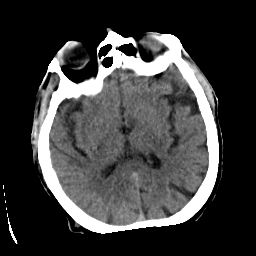
\includegraphics[width=13mm, height=13mm]{figs/013ct}
\end{minipage}
\end{tabular}}
& High-resolution global anatomical structure  of hard tissue
&\multirow{5}{*}{\begin{tabular}[c]{@{}c@{}}Global contour\\  lines; Local \\shape location \\of tiny area;\\More source \\image informat-\\ion\end{tabular}}
& \multirow{5}{*}{\begin{tabular}[c]{@{}c@{}}  Multi-scale; \\ Concatenate;\\
Gray color space\end{tabular}}
& \multirow{3}{*}{\begin{tabular}[c]{@{}c@{}} \\\\\\ GV-branch\end{tabular}}\\  \cline{2-2}
& High-resolution local anatomical  structure of hard tissue
& &  &    \\ \cline{1-2}

\multirow{2}{*}{\begin{tabular}[c]{@{}c@{}}\textbf{PET}\\
\begin{minipage}{0.09\textwidth}
\centering
      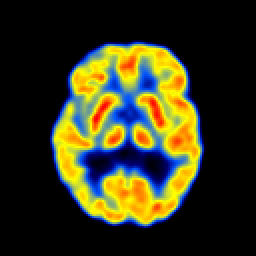
\includegraphics[width=13mm, height=13mm]{figs/013pet}
\end{minipage}
\end{tabular}}
& Obvious display of early small lesion
& &  &  \\ \cline{2-4}
& High-distinguished functional-metabolic abnormity tissue
& Brightness
& Brightness component of HSV color space & \\ \hline
\end{tabular}
\end{table*}
\fi
    \begin{figure*}[htb]
      \centering
          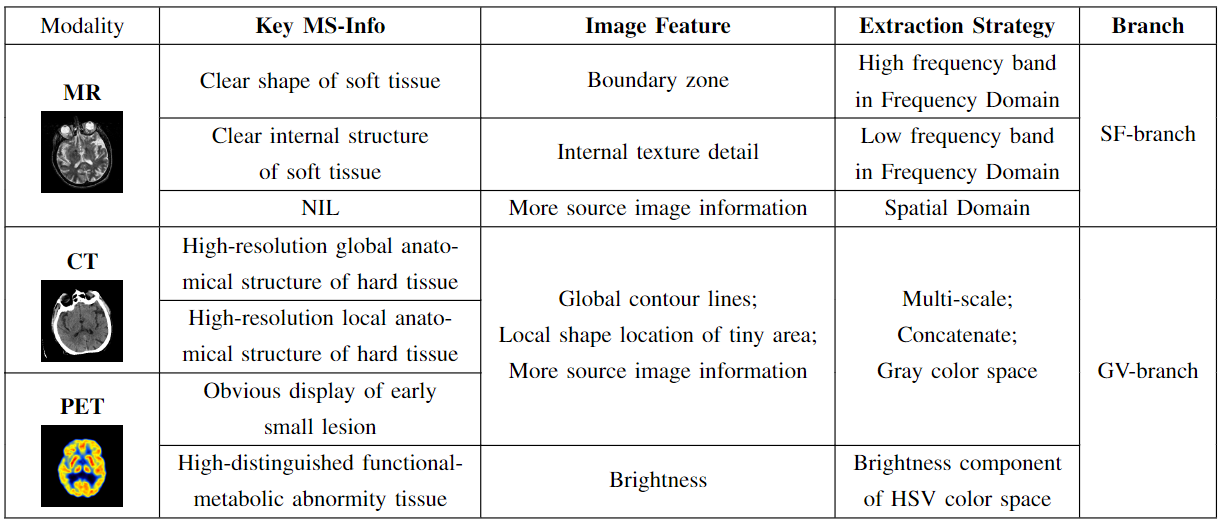
\includegraphics[width=0.9\columnwidth]{figs/paper1semanticfeature.png}
          \caption{多模态医学影像的关键医学语义信息引导两个特征提取分支的设计}\label{paper1semanticfeature}
     \end{figure*}
    
\subsection{医学语义引导的双分支网络}
不同模态的医学影像中包含着不同的医学语义信息(medical semantic information,MS-Info),这对临床疾病诊断具有重要意义。因此,应该保持和加强各自在其多模态医学影像融合结果的MS-Info。为了实现这一目标,本节首先根据临床医学和成像理论分析每种模态的MS-Info。然后,映射关键MS-Info到影像特征,并为不同的功能设计有效的提取策略。MRI/CT/PET/SPECT的关键医学语义信息如何指导MsgFusion的两个分支设计的细节在表\ref{paper1semanticfeature}中给出,其引导构建所提出的医学语义引导的双分支融合网络(Medical Semantic Guided Fusion,MsgFusion)的两个分支。

 \begin{figure*}[htb]
  \centering  %width=\columnwidth width=\textwidth
      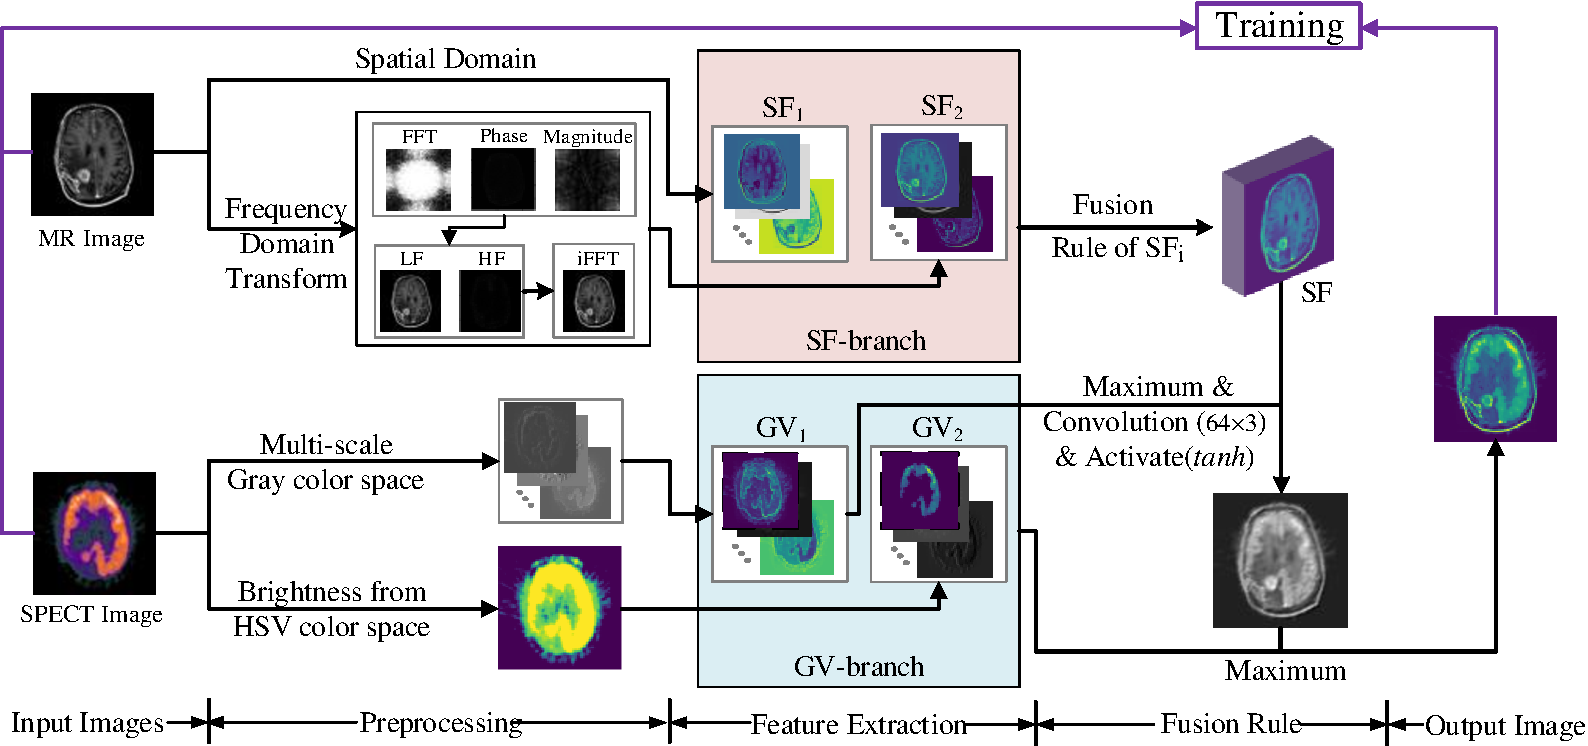
\includegraphics[width=0.9\textwidth]{figs/paper1framework_20221225.pdf}
      \caption{MsgFusion方法的框架:医学语义引导的多模态脑影像融合双分支网络}
      \label{paper1Framework}
 \end{figure*}
 
MsgFusion的整体框架如图\ref{paper1Framework}所示,其中预处理和特征提取是关键步骤。首先,在深度MS-Info提取阶段,网络结合了两个特征提取分支,空间域和频率域结合的分支(the branch combines spatial domain and frequency domain,SF-Branch)和灰度与自定义V分量结合的分支(the branch combines gray color space
and self-defined brightness information,GV-Branch),如图\ref{paper1Framework}所示。SF-Branch采用傅立叶变换,GV-Branch采用HSV颜色空间,不仅充分利用了影像的空间和频率关系,而且从影像的重要信息中提取了丰富的语义特征。第二,是本节的分层融合策略。这两个特征提取分支的结合不仅提高了算法的性能,而且有效地获得了多模态医学脑影像的重要的MS-Info。

\subsubsection{空间域和频率域结合的方案}
SF-Branch被设计用于从MRI中提取深度特征。如表\ref{paper1semanticfeature}所示,MRI的MS-Info,即,软组织的清晰形状和内部结构在频域中更容易区分为高频带信息和低频带信息。为了有效地提取MS-Info对应的深层特征和更多的源影像信息,本节采用了频域和空间域相结合的策略。图\ref{paper1AS_Fu}示出了SF-Branch的过程。
    \begin{figure*}[htb]
      \centering
          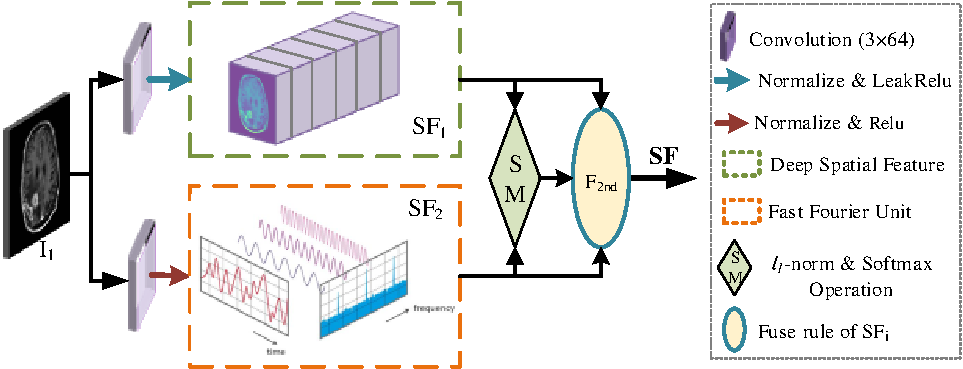
\includegraphics[width=0.9\columnwidth]{figs/paper1AS_Fu.pdf}
          \caption{SF-Branch提取特征的过程}\label{paper1AS_Fu}
     \end{figure*}
     
特征提取的SF-Branch包括两部分,一部分是从神经网络的卷积特性中获取源MRI的深层特征;另一部分是从频域中获取MS-Info对应的特征。在第一部分中,通道被放大到64,卷积核的大小设置为7 × 7,步幅设置为1,填充量为3。批量归一化并使用LeakyReLU(alpha=0.2,inplace=true)激活卷积特征。该部分的输出记录为$SF_1$,如图\ref{paper1AS_Fu}所示。另一部分先采用频域处理,其输出记为$SF_2$。频域处理的示例显示在由图\ref{paper1Framework}中用频域变换标记的箭头所指向的正方形中。具体地,一幅M × N影像的二维离散傅立叶变换和逆变换表示为等式(\ref{ftFunction})和式(\ref{iftFunction})。其中,$x$和$y$为空间域中的影像变量,$f(x,y)$表示点$(x,y)$处的灰度值,$u$和$v$为频率变量,当$u$和$v$为0时,为原点处的傅立叶变换,相当于一幅影像的平均灰度值。

    \begin{equation}\label{ftFunction} %离散傅里叶变换
     F(u,v)=\frac{1}{M N} \sum_{x=0}^{M-1} \sum_{y=0}^{N-1} f(x,y) e^{-j 2 \pi(u x / M+vy / N)}
    \end{equation}
    \begin{equation}\label{iftFunction} %离散傅里叶逆变换
     f(x,y)=\sum_{u=0}^{M-1} \sum_{v=0}^{N-1} F(u,v) e^{j 2 \pi(u x / M+v y / N)}
    \end{equation}

假设$Re$和$Im$分别用于表示$F$的实部的和虚部,则它们的计算是根据等式(\ref{RealPart})和等式(\ref{imaginaryPart}):

    \begin{equation}\label{RealPart}   %实部
      \sum_{x=0}^{N-1} \sum_{x=0}^{N-1} f(x,y) \cos \left(2 \pi\left(\frac{w x}{N}+\frac{v y}{N}\right)\right)
    \end{equation}
    \begin{equation}\label{imaginaryPart}  %虚部
       \sum_{x=0}^{N-1} \sum_{y=0}^{N-1} f(x,y) \sin \left(2 \pi\left(\frac{w x}{N}+\frac{v y}{N}\right)\right)
    \end{equation}

影像经过傅立叶变换后,每个像素都是一个包含实部的和虚部的复数。通过计算每个像素的复数的幅值和相位,可以得到影像的幅值和相位。傅立叶频谱、相位角和振幅被定义如下:
    \begin{equation}\label{amplitude}  %功率谱(幅度)
       P(u,v)=|F(u,v)|^{2}=Re(u,v)^{2}+Im(u,v)^{2},
     \end{equation}
    \begin{equation}\label{PhaseAngle} %相位角
     \phi(u,v)=\arctan \left[\frac{Im(u,v)}{Re(u,v)}\right],
    \end{equation}   
   \begin{equation}\label{spectrum}  %频谱
      |F(u,v)|=\left[Re(u,v)^{2}+Im(u,v)^{2}\right]^{\frac{1}{2}}.
    \end{equation}

这是首次使用傅立叶变换进行医学影像融合。傅里叶变换的作用是把影像的空间域灰度级分布转换成影像的频率域表示,逆傅里叶变换是将影像的频率表示变换回灰度分布级函数。通过傅立叶变换可以得到磁共振影像的幅值和相位。影像的幅度包含影像的全局信息,而相位包含影像的局部信息。利用傅里叶变换的性质,该方法能够取得较好的融合效果,并通过实际实验验证了该方案的切实有效性。

当完成上述步骤时,接下来本节需要在空间域和频率域之间融合特征。本文提出的加权图特征是融合多尺度深度特征来获得空间特征的详细结构。权重映射通过$l_1$范数和softmax运算通过目标函数完成,如下式(\ref{sbfunciton})所示:

 \begin{equation}\label{sbfunciton}
    \xi_{k}(x,y)=\frac{\left\|\operatorname{\psi}_{k}(x,y)\right\|_{1}}{\sum_{i=1}^{2}\|\operatorname{\psi}_{i}(x,y)\|_{1}},
    \end{equation}
    
其中,$\|\cdot\|_{1}$表示$l_1$-norm,$\mathrm{\emph{$k$}} \in 1$, $2$ 。 $(x,y)$,并且在深度特征中,每个位置对应一个维度为$dim$的向量表示。$\psi$表示具有$dim$维度的向量。最终的融合特征图$\varphi$,是两个增强的特征图的叠加,其由式(\ref{featuremap})表示:
 
    \begin{equation}\label{featuremap}
     \varphi =\sum_{i=1}^{2}  \xi_{{k}(x,y)}^{(i)} \times \psi_i.
    \end{equation}

\subsubsection{灰度与V颜色分量结合的方案}
GV-Branch设计用于从CT/PET/SPECT提取深层特征。一方面,GV-Branch采用灰度空间的多尺度级联策略,从源影像中提取全局轮廓和局部形状特征,补偿不同尺度下的信息损失。另一方面,根据表\ref{paper1semanticfeature}中的分析,PET/SPECT(高分辨功能代谢异常组织)的关键MS-Info主要反映在影像的亮度水平上。为了获得亮度信息,本节使用HSV颜色空间变换来计算V分量,并将其改进为新的亮度值以突出功能影像(PET/SPECT)的MS-Info。将CT的MS-Info(硬组织的高分辨率全局和局部解剖结构)和PET/SPECT的部分MS-Info(早期小病变的明显显示)引导到多尺度策略,在灰度颜色空间中级联。为了从不同的尺度和层次捕获信息,以较少的信息损失,采用了多尺度和跳跃连接策略。 CT不包含功能代谢信息。当CT输入到GV-Branch时,仅需要灰度颜色空间中的深度特征。总的来说,为了有效地提取对应于MS-Info和更多源影像信息的深度特征,本节采用了HSV颜色空间和灰度颜色空间相结合的策略。
     \begin{figure}[htbp]
      \centering
      % Requires \usepackage{graphicx}
          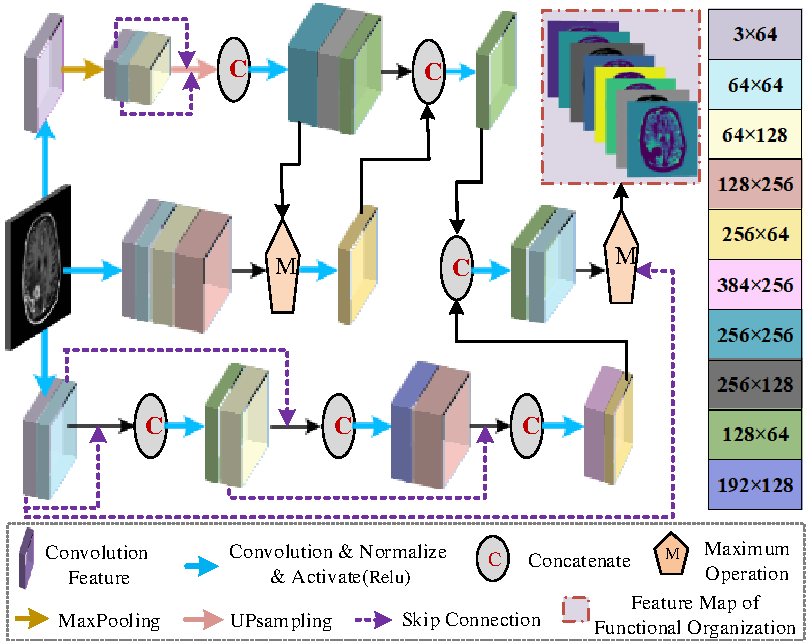
\includegraphics[width=0.9\columnwidth]{figs/paper1cb_work.pdf}
          \caption{GV-Branch提取特征的过程一}\label{paper1cb_work}
     \end{figure}
     
1)通过多尺度策略获得深度卷积特征:由于不同层次和分辨率的卷积运算可以提取不同重要程度的信息,因此提出了一种针对脑影像的功能组织特征提取方法。该方法的功能组织特征分支网络如图\ref{paper1cb_work}所示。网络块主要包括卷积层、池化层、上采样和跳跃连接操作。图\ref{paper1cb_work}给出了获取MS-Info的具体步骤,不同的色块表示不同数量的输入和输出通道,其对应于不同厚度。

多次使用拼接可以扩展高维特征,更准确地发现更重要的语义特征。当多条分支合并时,采用最大值法突出高频纹理信息。由于各种脑部疾病是不均匀的,使用这种特征提取策略可以使病变程度和正常组织之间的分类更加明显。然后,可以更容易地确定PET影像中的局部区域是否异常,并在CT影像中观察到清晰的轮廓和全局结构信息。并且,使用长短跳来增强图\ref{paper1cb_work}中带有紫色虚线的特征的转移,可以充分融合不同层次的视觉特征,减少特征转移过程中的特征损失。这个想法受到DenseNet\cite{2016Densely}的启发,DenseNet主要由许多密集的网络块实现。为了解决消失梯度问题,网络只级联卷积操作的前后层的权重系数,而不级联池化操作。在本节的网络中,将前一层和前一层的特征输入到下一层,连接模态表示为式(\ref{skipfunciton}):

     \begin{equation}\label{skipfunciton}
        f_{d}=H_{d}([f_{0},f_{1},...,f_{d-1}]),
     \end{equation}
     
   \begin{figure}[htb]
      \centering
      % Requires \usepackage{graphicx}
          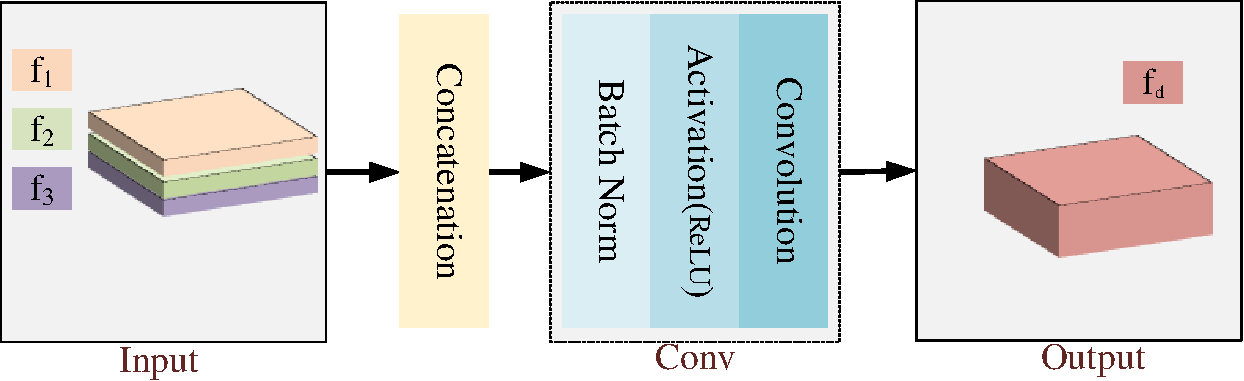
\includegraphics[width=0.9\columnwidth]{figs/paper1skip.pdf}
          \caption{特征跳跃策略}\label{paper1skip}
     \end{figure}
     
其中,$f$表示输出,$d$表示网络中的层数,$H_{d}(*)$表示非线性传递函数的组合,包括级联、BN、激活和卷积操作。多层特征(不一定是相邻层)的并行输入由组合函数操作以获得新特征。新特征的通道数由不同的卷积参数决定。详细步骤如图\ref{paper1skip}所示。此操作有助于捕获跨区域的长期和多层依赖关系,并减少特征转移过程中的损失。因此,可以保留更完整的脑影像结构。


2)通过颜色空间变换获取亮度信息:HSV颜色模型,基于对色彩的直觉理解构建而成,由色调(Hue)、饱和度(Saturation)和亮度(Value)三个参数组成,并以其几何表示而著称于六角锥体模型。HSV颜色空间可以单独处理,并且彼此独立。因此,通过采用HSV颜色模型进行影像分析与处理时能够显著降低复杂度,并且相比RGB色彩空间,HSV更贴合人类视觉系统的自然感知方式。在此特征提取部分,本节计算功能影像的HSV空间的V分量,以提取其亮度特征用于后续处理,如图\ref{paper1FO2_hsV}所示。在该图中,$I_p$表示原始RGBA影像,$I_A$表示RGB影像,$V$表示将$I_p$变换到HSV空间之后的亮度分量。为了进一步增强亮度明显区域的局部信息,本节定义了一个新的亮度值$V'$,如算法\ref{paper1algorithm1}所示。 
   \begin{figure}[htbp]
      \centering
      % Requires \usepackage{graphicx}
          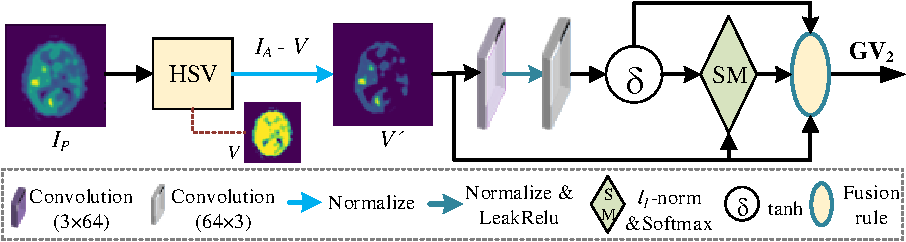
\includegraphics[width=0.9\columnwidth]{figs/paper1FO2_hsV.pdf}
          \caption{GV-Branch提取特征的过程二}\label{paper1FO2_hsV}
     \end{figure}


    \begin{algorithm}[ht]
    \caption{New Luminance Computation}\label{paper1algorithm1}
    \centering
    \begin{algorithmic}[1]
    \Require RGBA image $I_p: (R, G, B, A)$
    \Ensure New luminance value $V'$
    %\STATE
    \State {\textbf{newLum}} $(I_p)$:
    \State \hspace{0.5cm}$I_{A} \gets$ \text{Compress} $(I_p)$;
    \State \hspace{0.5cm}$I_{HSV}: (H, S, V) \gets$ \text{Conver} $(I_p)$;
    \State \hspace{0.5cm}$V' \gets$ $I_{A} - V$;
    \State \hspace{0.5cm}\textbf{return} $V'$;
    %\STATE 
    \State {\textbf{Compress}} $(I_p)$:
    \State \hspace{0.5cm}$I_{A} \gets$ $I_p:(R) + I_p:(G) + I_p:(B)$;
    \State \hspace{0.5cm}\textbf{return} $I_{A}$;
    %\STATE
    \State {\textbf{Conver}} $(I_p)$:
    \State \hspace{0.5cm}$I_{A} \gets$ \text{Compress} $(I_p)$;
    \State \hspace{0.5cm}$I_{HSV} \xleftarrow{Eq.~(\ref{Hcomponent})} I_{A}$;
    \State \hspace{0.5cm}\textbf{return} $I_{HSV}: (H, S, V)$;
    \end{algorithmic}
    \end{algorithm}

如图\ref{paper1FO2_hsV}所示,$I_p$是PET影像的一部分。图中可以发现三个不同的色块(黄色,浅绿色和深蓝色),它们表明能量高或新陈代谢旺盛的区域。病变最有可能存在于这些区域。这些颜色块可以从$I_p$的前景中辨别出来,主要是因为它们的亮度信息。然而,从亮度影像$V$中可以看出,这些有意义的区域还不够清晰,无法准确地定位病变。在算法 \ref{paper1algorithm1}中,本节通过$I_A-V$计算差分影像,以进一步突出这些色块。然后,病变可以清楚地定位在$V'$影像的右侧。基于新的亮度影像,通过后续过程提取HSV颜色空间中的深度特征$GV_2$,如图\ref{paper1FO2_hsV}所示。
  
  
\subsubsection{双分支的分层融合与重构}
为了充分利用从两个分支中提取的深层MS-Info特征,本节采用了基于分类和分层的融合策略,如图\ref{paper1Framework}的融合规则阶段所示。在第一层融合解剖结构特征(SF和GV$_1$),然后在第二层融合功能代谢特征(GV$_2$),有利于保留和增强待融合医学影像的关键MS-Info。本节的融合策略不是一个简单的加权和。为了保持和增强多模态影像的重要纹理特征,使用最大化操作。同时,使用卷积和激活函数来获得局部细节结构特征。如图\ref{paper1Framework}所示,采用$tanh$作为激活函数。 


\subsubsection{损失函数构建及参数设置}
由于医学数据的保密性,大量的多模态医学数据不易获取。通常,许多基于ImageNet数据训练的网络模型,如ResNet\cite{2016Inception}和VGG\cite{2015Places205},被选择来生成预训练参数。为了在解决梯度破碎问题和收敛速度方面获得更好的性能,本节选择ResNet101来迁移ImageNet上的最后一个卷积特征,也就是说,使用在ImageNet数据上预训练的ResNet101的最后一层作为本节的第一个卷积层来提取有效的影像特征。由于预训练模型是针对分类任务设计的,因此在本节的网络结构中,第一层的参数会根据本节的任务进行调整,以达到更好的融合效果。为了获得源影像的更精确的重建,本节联合结构和像素信息来构造损失函数如下式(\ref{paper1loss_function}):
     \begin{equation}\label{paper1loss_function}
       L=\omega L_{S} + (1-\omega)L_{P}
      \end{equation}

总损失函数由结构相似度$L_{S}$和像素损失$L_{P}$组成,$\omega$为调整系数,其值由训练和测试效果根据不同取值而定。$I_f$表示融合的结果,$I_i,i=1,2$表示输入的源影像。SSIM表示两个影像的结构相似性[44]。对于这两种类型的影像,计算结构相似度并将其组合。假设两个影像的结构相似度为$F_{SSIM_i}$,$F_{SSIM_i}= 1-SSIM(I_f,I_i),i=1,2$,总结构相似度函数计算如下:

     \begin{equation}\label{paper1L_{SSIM}}
        L_{S}=\sum_{i=1}^2\alpha_i\left(1-\frac{\left(2 \mu_{I_f} \mu_{I_{i}}+c_{1}\right)\left(2 \sigma_{I_f}\sigma_{ I_{i}}+c_{2}\right)}{\left(\mu_{I_f}^{2}+\mu_{I_{i}}^{2}+c_{1}\right)\left(\sigma_{I_f}^{2}+\sigma_{I_{i}}^{2}+c_{2}\right)}\right)
      \end{equation}
其中,$\mu_{I_f}$是$I_f$的平均值,$\mu_{I_{1}}$和$\mu_{I_{2}}$分别是$I_{1}$和$I_{2}$的平均值。$\mu_{I_f}^{2}$是$I_f$的方差,$\mu_{I_{1}}^{2}$和$\mu_{I_{2}}^{2}$分别是$I_{1}$和$I_{2}$的方差。$\sigma_{I_f I_{1}}$和$\sigma_{I_f I_{2}}$是原始影像和融合影像之间的协方差,$c_{i}$是常数。像素损失是$l_{2}$范数。假设两幅影像的像素损失为$F_{M_i}$,$F_{M_i}= \left\|I_f-I_i \right\|_2$,则总像素损失函数计算如下:

      \begin{equation}\label{paper1L_{P}}
       L_{P}= \beta \sum_{j=1}^{n}\left(I_{f_{j}}-I_{1_{j}}\right)^{2}+
       (1- \beta)\sum_{j=1}^{n}\left(I_{f_{j}}-I_{2_{j}}\right)^{2}
      \end{equation}
在式(\ref{paper1L_{SSIM}})和式(\ref{paper1L_{P}})中,$\alpha_i,i=1,2$,$\beta $是设置在区间$[0,1]$中的权重参数。在本节中,这三个参数都设置为0.5。在方程式(\ref{paper1loss_function})中,$\omega\in[0,1]$的取值由训练效果和测试效果决定。参数$\omega$决定了不同模态原始影像与融合结果影像之间相关性的程度。在其他参数不变的情况下,通过观察不同$\omega$的融合影像的效果来确定它的取值,如图\ref{difOmega}所示。
   \begin{figure}[htbp]
      \centering
      % Requires \usepackage{graphicx}
          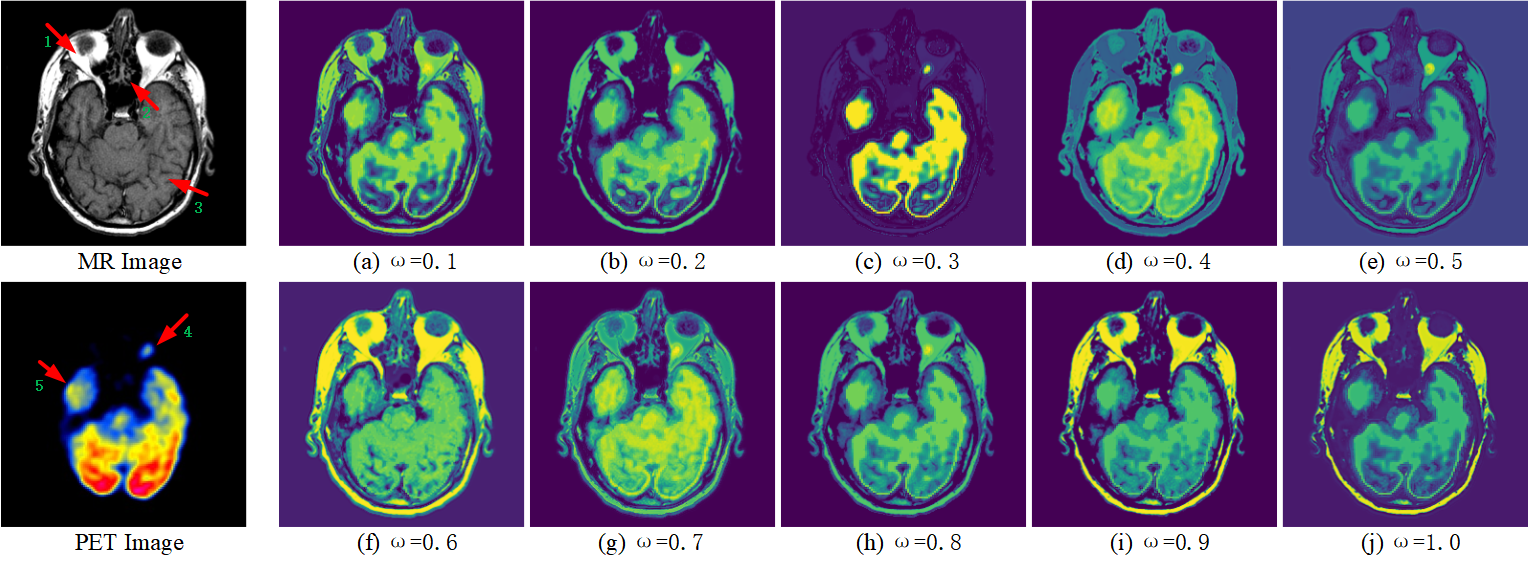
\includegraphics[width=0.9\columnwidth]{figs/difOmega.png}
          \caption{不同的$\omega$值应用于MRI-PET影像融合的结果 }\label{difOmega}
     \end{figure}
     
\begin{table*}[ht]
\centering
\caption{针对不同$\omega$取值下的MRI-PET影像融合的质量评估}\label{difOmega_evaluation}
\begin{tabular}{m{2cm}<{\centering}m{3cm}<{\centering}m{3cm}<{\centering}m{3cm}<{\centering}} 
\hline
\textbf{$\omega$} & \textbf{EN}     & \textbf{SD}      & \textbf{VIF}   \\\hline
0.1        & 3.3390          & 46.1341          & 0.2065          \\
0.2        & 3.1554          & 44.4309          & 0.2087          \\
0.3        & 3.2173          & 47.9444          & 0.0395          \\
0.4        & 3.7952          & \textbf{51.3496} & 0.2017          \\
0.5        & 4.0602          & 26.4541          & 0.0443          \\
0.6        & \textbf{4.5183} & 46.2509          & 0.2243          \\
0.7        & \textbf{4.3093} & \textbf{51.8038} & \textbf{0.2801} \\
0.8        & 3.1933          & 45.3808          & 0.2378          \\
0.9        & 3.1667          & 47.9978          & \textbf{0.2871} \\
1.0        & 3.9747          & 35.0954          & 0.1738      \\ \hline   
\end{tabular}
\end{table*}
本节通过实验来解释$\omega$的影响,并为$\omega$设置了一组值{0.1,0.2,0.3,0.4,0.5,0.6,0.7,0.8,0.9,1.0}。在图\ref{difOmega}中,第一列显示了MRI和PET影像,其他影像是采用不同$\omega$的融合结果。从图中可以直观地观察到,当$\omega$小于0.5时,融合结果中的MRI信息损失更大,尤其是当0.3最严重。当$\omega$大于0.5时,融合结果中PET的亮度信息或多或少会丢失或失真。只有当$\omega$为0.7时,PET的亮度信息才能得到最好的保留,MRI的边缘轮廓信息也很清晰。
表\ref{difOmega_evaluation}显示了图\ref{difOmega}中不同$\omega$下MRI-PET融合的三个指标。EN表示信息熵,SD表示标准差,VIF是对人类视觉感知的评估。这三个值越大,融合影像质量越好。融合影像质量评估指标的计算结果与上述观察结果一致。当$\omega$为0.7时,三个指标值达到最佳平衡和优化状态,其中SD最好,EN和VIF接近最佳值。


综上所述,当$\omega$取0.7时,得到的结果最好。因此,本节在实验中选择该值来测试融合效果。在训练过程中,初始学习率为0.001,250 epoch,批量大小为2,采用批量归一化,优化函数为Adam。此外,本节实施了一种自适应损失调整方案,即每隔50个训练周期将学习率调整为初始值的10\%,因为在训练过程中使用较小的学习率来调整权重以获得更好的权重。本节的方法已经在PyTorch版本1.5.0及其相应的CUDA版本10.1下的Python 3.7.9中实现。

\subsection{多模态脑影像融合的实验}
为了进一步验证所提出融合技术的效能,实验在不同的大脑影像对(MRI-SPECT/MRI-CT/MRI-PET)上进行。从ADNI(http://adni.loni.usc.edu/data-samples/access-data/)中获得了总共555个MRI-PET影像对作为训练集,其大小为256×256。在测试MRI-CT、MRI-SPECT和MRI-PET影像对中使用了全脑图谱 (http://www.med.harvard.edu/aanlib/)上的30对影像,包括脑血管疾病(中风)和肿瘤疾病(脑肿瘤)。所有实验都在GeForce RTX 3090 Ti 12 Intel Core Interl(R)Xeon(R)CPU E5-2678 v3 2.50 GHz 64 GB RAM设备的GNU/Linux x86 64系统上进行。

对于每对影像的实验,本节使用所提出的MsgFusion和其他九种代表性的方法(LatLrr\cite{2018Infrared},IFCNN\cite{2020IFCNN},NestFuse\cite{2020NestFuse},atsIF\cite{2020An},FusionDN\cite{2020FusionDN},FusionGAN\cite{2019FusionGAN},FunFuseAn\cite{kumar2019structural},WPADCPCNN\cite{panigrahy2020mri}和OLTPSpS\cite{das2022optimized})得到融合结果。并采用EN\cite{roberts2008assessment}、SD\cite{shi2005wavelet}
、MI\cite{qu2002information}、rSFe\cite{2007A}、SM\cite{Piella2003IP}、VIF\cite{han2013new}等6种常用的评价指标和一种相对新颖的指标$R_{Q}^{(F/(AB))}$(简称RQ)\cite{sengupta2020edge}来评价这10种方法的融合效果。RQ通过计算分数阶微分来反映融合影像中保留了多少边缘信息,它取代了\cite{Xydeas2000Objective}中使用的噪声敏感的Sobel算子,文章中采用三个Sigmoid函数(tanh、arctan、Logistic)来得到三个度量。考虑到它们共同的函数单调性,本节只选择了一个基于Logistic函数的度量应用于本节的实验中。由于不同指标的值相差很大,本节进行了适当的线性变换,图\ref{paper1MPDindex}和图\ref{paper1CMDindex}的左上角标出了这些变换,以方便在同一图中进行比较。

\subsubsection{MRI-SPECT影像对的融合}
图\ref{paper1mpd008roi}中的第一列显示源MRI和SPECT影像。MRI清晰显示脑脊液和其他软组织的纹理细节。SPECT上的不同颜色和亮度可以反映代谢信息。图\ref{paper1mpd008roi}(a)-(i)示出了所考虑的十种融合方法的结果。图\ref{paper1mpd008roi}(j)展示出了通过MsgFusion获得的融合结果。聚焦于由七个箭头指示的区域,可以看出,与由其他七种方法获得的融合影像中的对应区域相比,显示出更清晰的结构和纹理细节。结合临床信息,本节分析了MRI和SPECT的MS-Info是否很好地保留在图\ref{paper1mpd008roi}(j)中蓝色矩形框内箭头指示的7个区域的融合结果中。

     \begin{figure*}[ht]
      \centering
       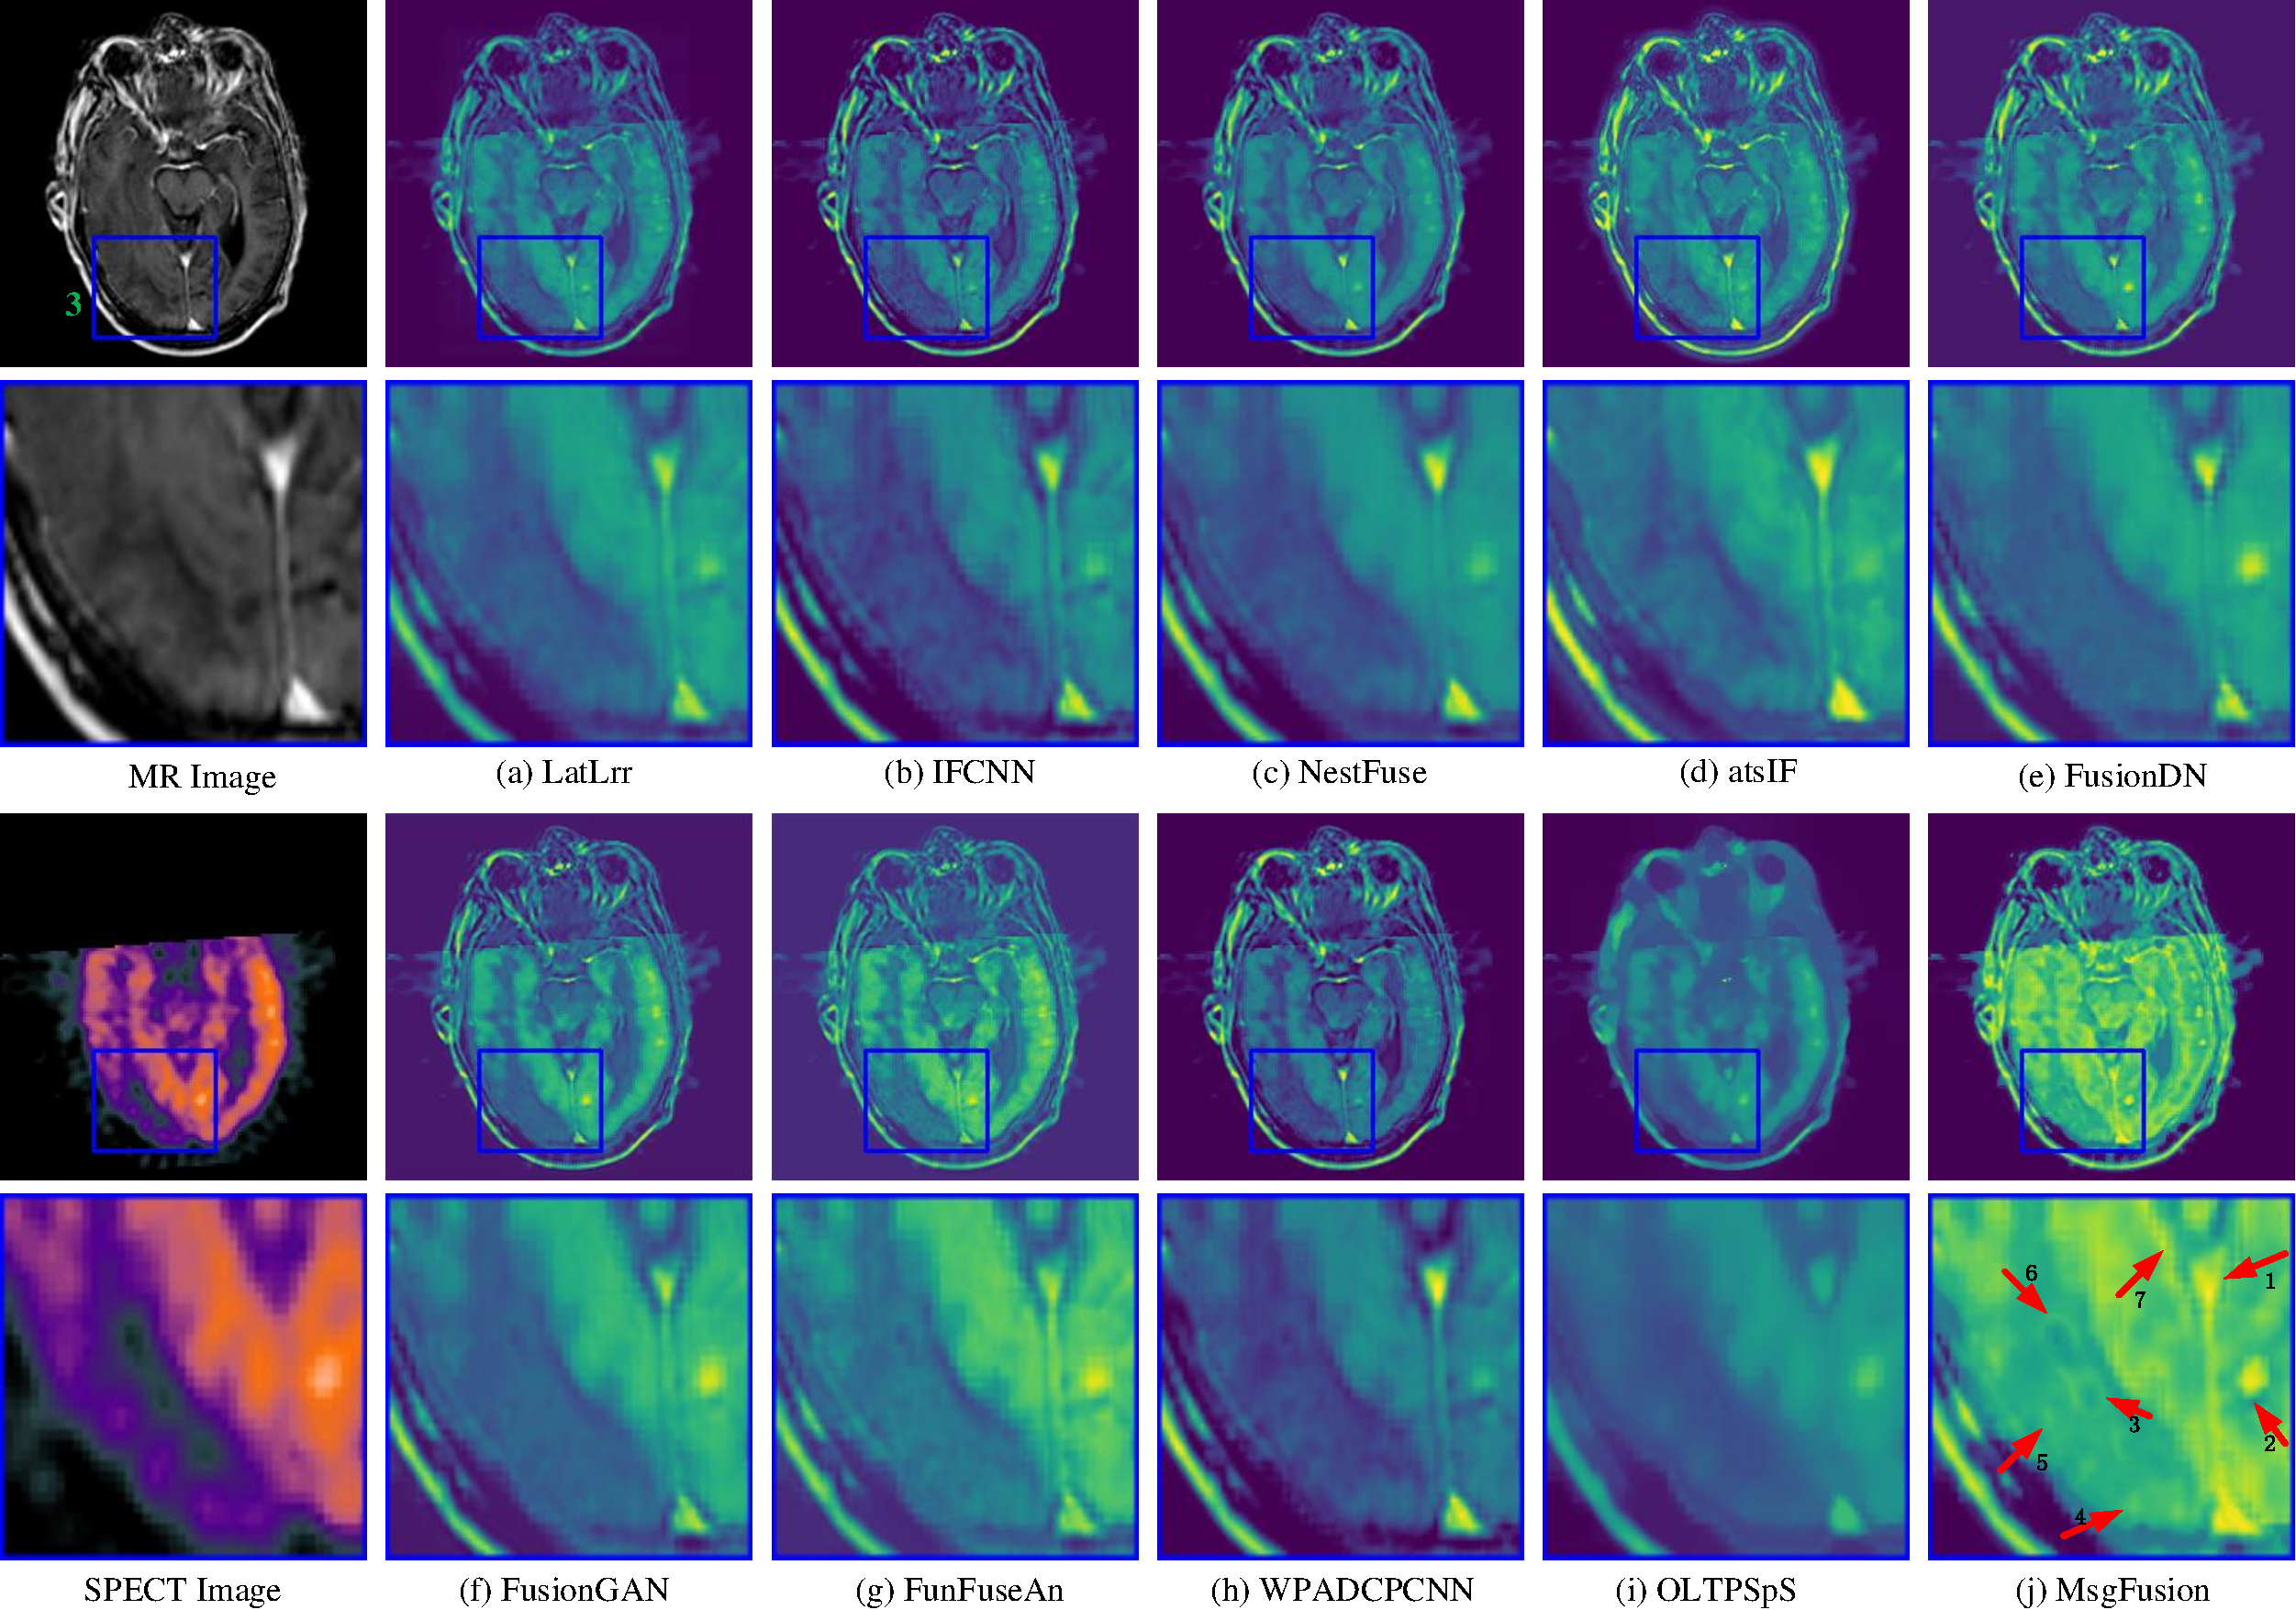
\includegraphics[width=0.9\textwidth]{figs/paper1mpd008roi.pdf}
      \caption{用于脑MRI-SPECT影像融合的不同方法(LatLrr、IFCNN、NestFuse、atsIF、FusionDN、FusionGAN、FunFuseAn、WPADCPCNN、OLTPSpS和本节提出的MsgFusion)性能比较} \label{paper1mpd008roi}
     \end{figure*}
     
箭头1指向小脑结节区域,MRI源影像上可见一个轮廓清晰的白色小三角形,右上角略有模糊。然而,在SPECT源影像中,没有明显的特征。在LatLrr的融合结果中,影像显得模糊,与周围组织无法区分。在IFCNN、NestFuse和FusionDN的融合结果中,它们都比SPECT保留了更多的MRI信息。右上角的增强效果不明显。FusionGan和FunFuseAn结果中的小三角形扭曲。在OLTPSPS的融合结果中,亮度信息明显丢失。

箭头2为左小脑半球区域,主要来自SPECT影像,表现为边缘模糊的亮点,在MRI上看起来像一个小黑洞。在LatLrr、IFCNN、NestFuse、atsIF、WPADCPCNN和OLTPSpS的融合结果中,不容易找到那个亮点。在FusionGAN和FunFuseAn的融合结果中,亮点增强,但略有模糊。在FusionDN的融合结果中,这一亮点很明显,但与周边机构融合,具体位置无法确定。MsgFusion的融合结果中,有明显的亮度和轮廓,位置准确。

箭头3和6代表右小脑半球区域。在MRI中,它是具有灰度值,形状像一片树叶。在SPECT影像中,有三个相邻的灰色空环。从SPECT影像中可以发现,在箭头6指示的位置有一个清晰的灰色空环。在NestFuse和atsIF获得不均匀分布区域的融合影像中可以识别它,但不是很清晰,箭头3处的环消失不见。在IFCNN、FusionDN、FusionGAN、FunFuseAn和WPADCPCNN的融合结果中,它们在第6个ROI的环更清晰,而在第3ROI则不清晰。在本节提出的方法中,几个环可以很好地显示出来,并且很容易找到它们的位置。

箭头4和5分别是枕骨和右小脑半球的边缘区域。MRI中的这个区域看起来像花边,但不容易检测到。它在SPECT中表现为一个不明显的亮度小点。相比之下,MsgFusion保留了MRI的边缘,并且可以很容易地在SPECT中找到几个点。区域7是小脑结节附近的右鞍半球边缘。在由浅白色边缘信息表示的MRI中,在SPECT影像中似乎存在一条直线。对于所有方法的不同结果中,只有MsgFusion可以清楚地找到其边缘。

    \begin{figure}[ht]
      \centering
      % Requires \usepackage{graphicx}
          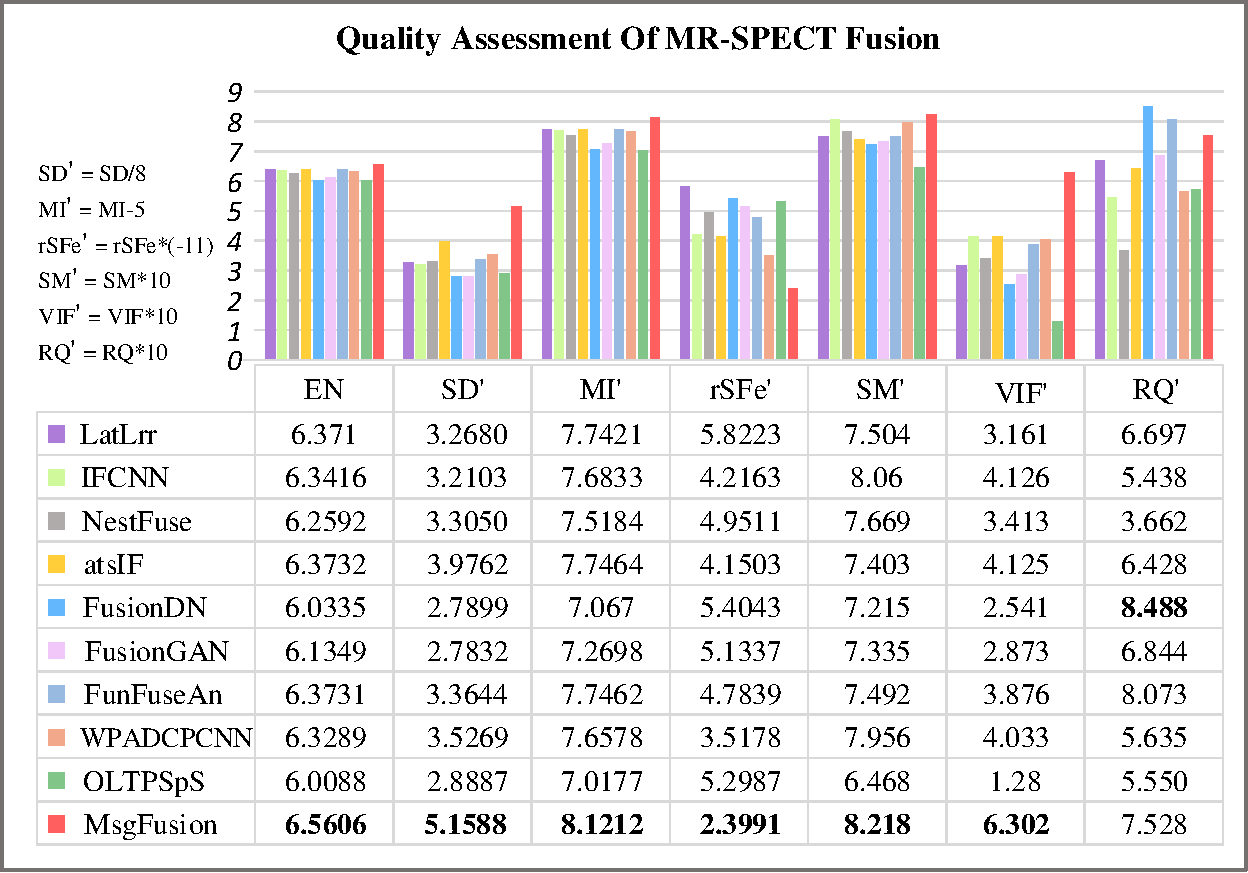
\includegraphics[width=0.9\columnwidth]{figs/paper1MPDindex.pdf}
          \caption{计算不同方法对MRI-SPECT融合的质量评估指标值}\label{paper1MPDindex}
     \end{figure}

图\ref{paper1MPDindex}显示了图\ref{paper1mpd008roi}中融合结果的评估指标,不同的颜色柱条对应不同融合方法。EN、SD、MI、SM、VIF、RQ分别表示融合的熵、标准差、互信息、结构相似度、视觉信息保真度和边缘信息,这些值越大,融合效果越好。rSFe反映了改善的空间频率,其绝对值越小,融合效果越好。除RQ外,其他6个评价指标均表明MsgFusion方法达到最佳融合效果。因此,本节的融合结果具有更合适的亮度、更清晰的轮廓和更精细的纹理。此外,本节的结果保持并增强了重要的医学信息。当大脑出现异常时,可以通过观察SPECT的颜色和亮度信息,并结合MRI的纹理进行有效的分析,来确定可能的疾病类型。

\subsubsection{MRI-CT影像对的融合}
图\ref{paper1cmd010roi}中的第一列显示了原始CT和MRI。很容易在CT影像上找到硬轮廓,如骨骼,在MRI上找到软组织结构。右边是不同融合方法的结果。图\ref{paper1cmd010roi}(j)展示出了MsgFusion的融合结果和获得的局部放大影像,主要关注由箭头指向的六个ROI。

    \begin{figure*}[ht]
      \centering
      % Requires \usepackage{graphicx}
          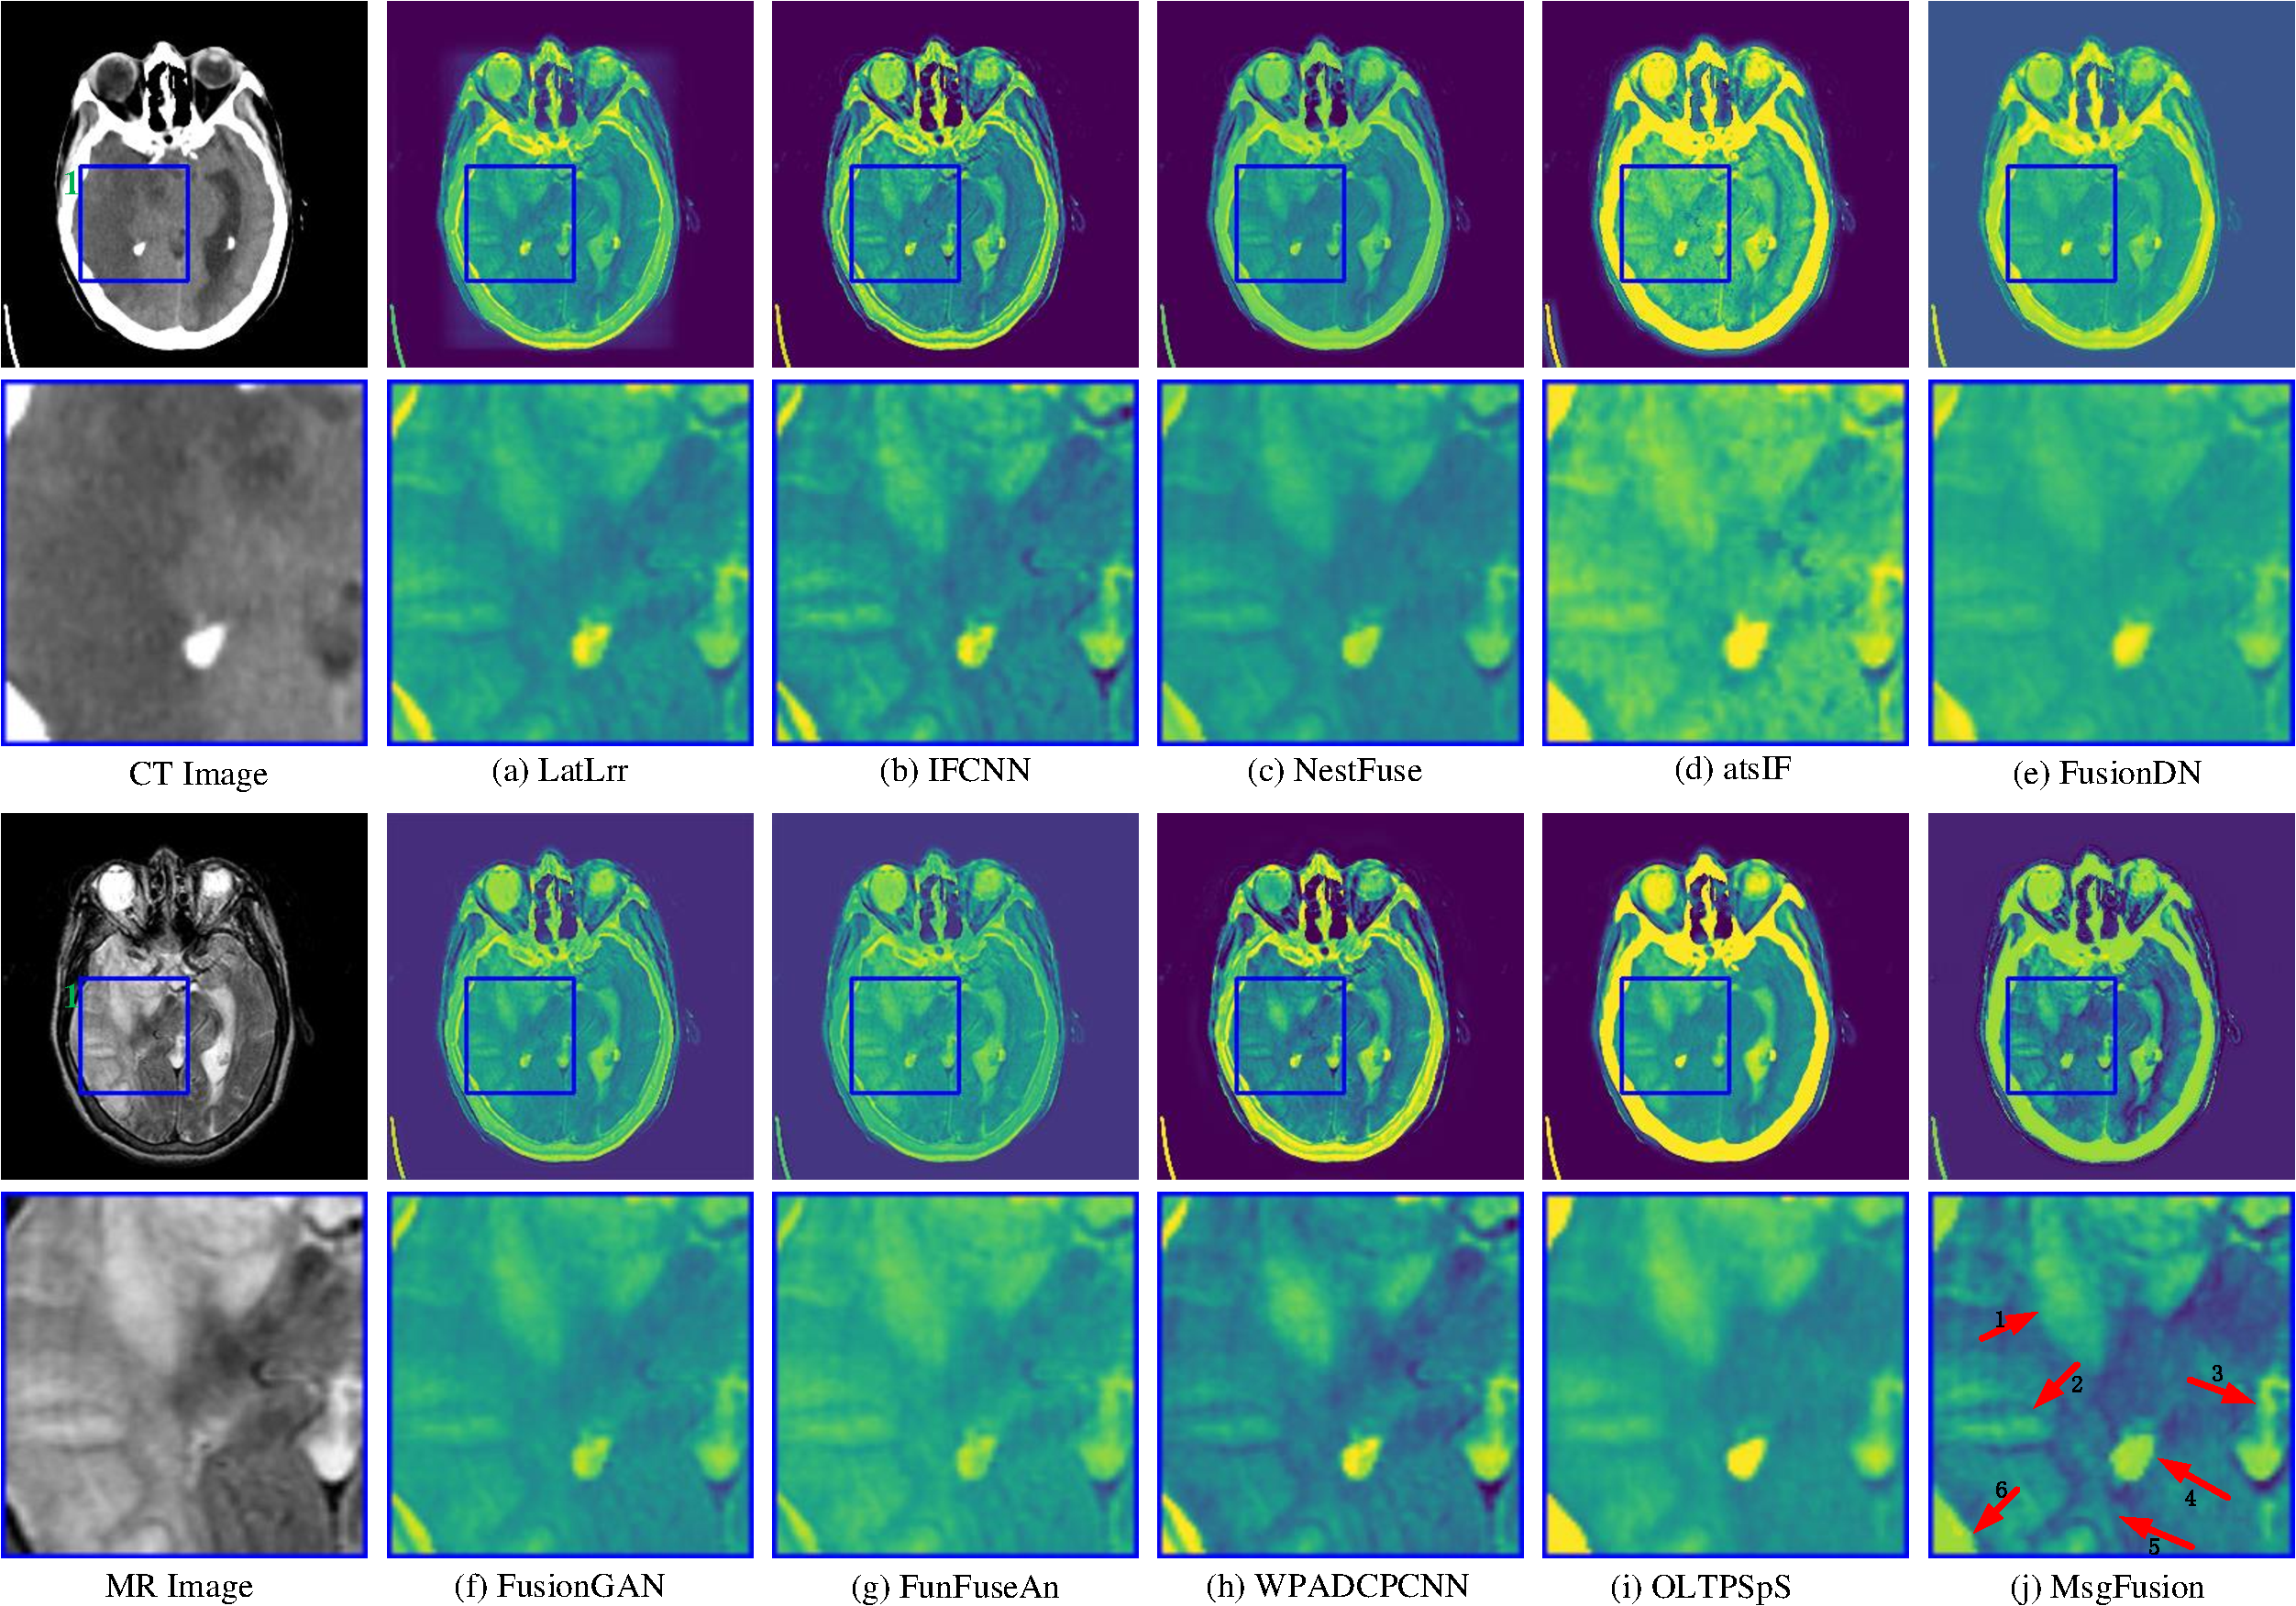
\includegraphics[width=0.9\textwidth]{figs/paper1cmd010roi.pdf}
          \caption{用于脑MRI-CT影像融合的不同方法(LatLrr、IFCNN、NestFuse、atsIF、FusionDN、FusionGAN、FunFuseAn、WPADCPCNN、OLTPSpS和本小节提出的MsgFusion)性能比较}\label{paper1cmd010roi}
     \end{figure*}

箭头1指向的区域代表侧脑室的下角,在CT影像上为深灰色,在MRI上为明亮而清晰。MRI中ROI 1的面积较大,具有重要的MS-Info信息,常被用来判断是否存在病变。在LatLrr、IFCNN、FusionDN、FunFuseAn和OLTPSps的融合结果中,轮廓不明显且不容易找到。在atsIF结果中,位置的亮度得到改善,但边缘出现了平滑现象。在FusionGAN和WPADCPCNN的融合结果中,位置的边缘分类明显,但亮度不够。在本文的融合结果中,可以很容易地找到区域及其边界。箭头2指向的区域呈岛状,主要反映在MRI上。这一区域并不像正常脑部影像中显示的那样完整,这表明组织失去了水分或萎缩。在图\ref{paper1cmd010roi}中可以发现,只有MsgFusion融合结果中的区域明显,并显示出有别于其他组织的清晰轮廓。箭头3指向的区域在CT影像上为第四脑室,在MRI上也有脑桥和基底动脉的部分信息相连。atsIF方法的亮度具有良好的亮暗影像对比度,然而,该区域的结构完整性被破坏。ROI 3中的其他算法的结果清晰但不够明亮,而WPADCPCNN和MsgFusion更好。

箭头4指向的区域为侧脑室后角,主要表现在CT影像上。它在MRI上不是特别明显,但是,通过与周围组织仔细区分可以发现。对于LatLrr、IFCNN、Nesthood和FusionGAN,可以找到ROI 4的轮廓,但其边界附近存在伪影,亮度信息不足。对于FusionDN,这个位置很明显,但周围组织丢失。FunFuseAn融合结果表明,融合区域变得模糊。OLTPSpS的结果有足够的亮度,但面积略小。在本节提出的方法中,ROI 4不仅具有清晰的轮廓和明显的边界,而且具有足够的亮度。在本节提出的方法中,侧脑室后角的重要医学特征存在并得到增强。

箭头5指向的区域为中央沟,主要表现在MRI上。该位置的密度和亮度信息可以帮助医生确定是否存在异常。对于MsgFusion区域,它具有清晰的轮廓和亮度信息,很容易找到。箭头6指向的区域为顶骨,主要在CT影像上反映。当这个区域有边缘缺损或不完整时,就可以判断是否有脑损伤。通过以上分析,可以表明MsgFusion具有相对更好的融合效果。

  \begin{figure}[ht]
      \centering
      % Requires \usepackage{graphicx}
          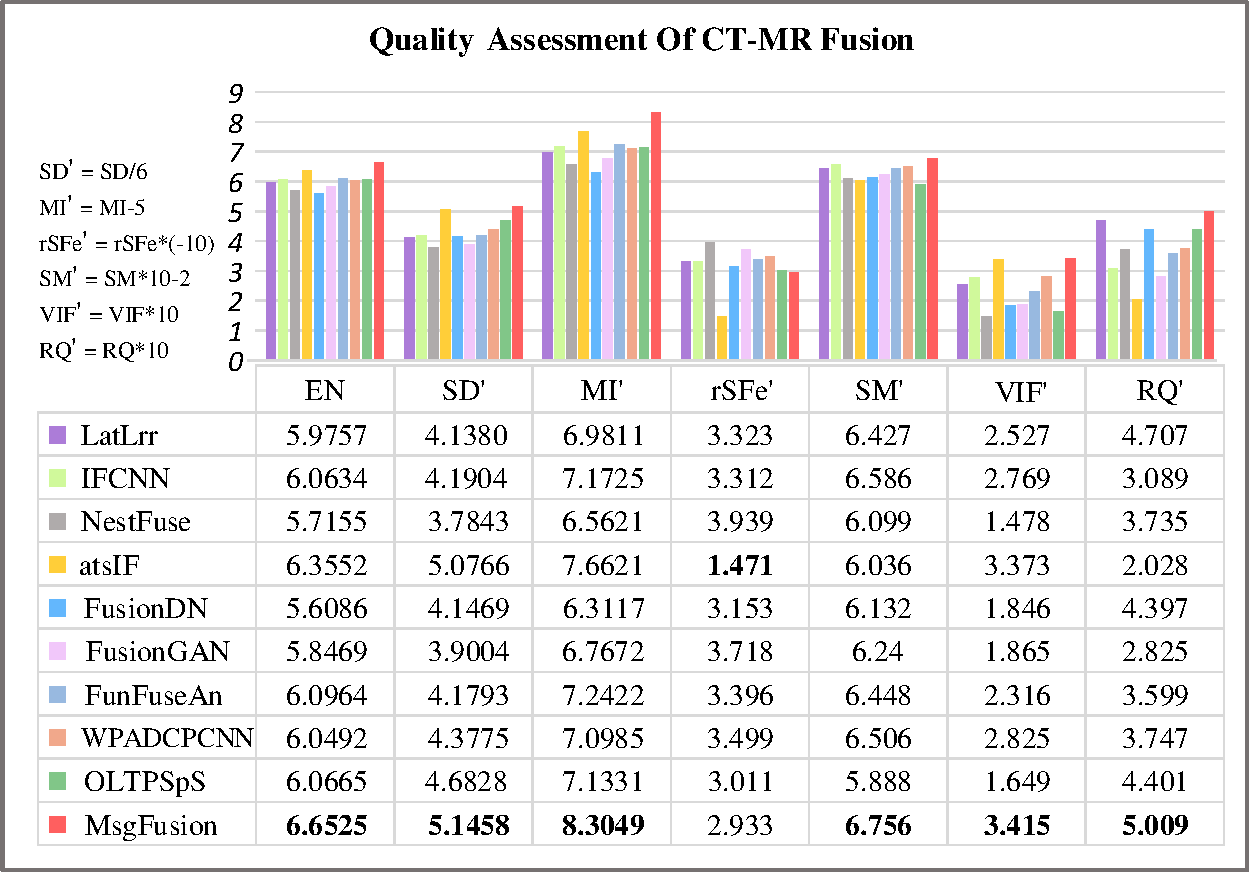
\includegraphics[width=0.9\columnwidth]{figs/paper1CMDindex.pdf}
          \caption{计算不同方法对MRI-CT融合的质量评估指标值}\label{paper1CMDindex}
     \end{figure}
     
此外,图\ref{paper1CMDindex}展示出了对应于图\ref{paper1cmd010roi}的质量评估指标值。结果表明,本节的MsgFusion方法在6个指标值上占优势,在rSFe上是次优的。这意味着原始CT和MRI的信息不仅保持良好,而且在本节的方法的融合结果中也得到了增强。当通过观察MRI密度和面积可以确定脑出血时,CT影像可以发现脑出血的大致范围。


%\subsubsection{计算成本}
%在我们的计算环境下,用10种方法对30对不同的数据形态进行了测试。记录每个方法的平均运行时间。所有结果都列在表\ref{paper1timeCost}中。我们可以看到,我们方法的平均运行时间是2.0048秒。虽然这不是一种快速的方法,但时间成本是可以接受的。

\if 0
  \begin{table}[ht]
    \centering
    \caption{影像融合方法的运行时间(单位:s)}\label{paper1timeCost}
    %\footnotesize
    \begin{tabular}{ccccc}
    \toprule[1pt]
     LatLrr &IFCNN &NestFuse &atsIF &FusionDN \\ \hline
     %1238.7976  &6.7223 &29.2867   &203.9445   &20.6184 \\ \hline
     41.2933  &0.2241 &0.9762   &6.7982   &0.6873 \\ \hline
     FusionGAN  &FunFuseAn &WPADCPCNN &OLTPSpS &MsgFusion\\ \hline
     %14.7726  &10.7955 &1190.1147 &1457.83 &60.1435\\
     0.4924  &0.3599 &39.6705 &48.59 &2.0048\\
    \bottoMRIule [1pt]
    \end{tabular}
 \end{table}
\fi

\subsubsection{影像融合的问卷调查}
对于医学影像融合,最终的目标是为医生提供易于观察的融合影像,以便对病变进行定性、定量和定位分析。因此,这种主观评价可以证实MsgFusion方法在临床意义上的优势。为了验证算法的临床有效性,本节对融合效果进行了在线问卷调查,并分发给了不同医院神经内科和医学影像科的30名医生。这些医生的临床经验:10年以上15人,5-10年3人,3-5年6人,3年以下6人。在这份问卷中,本节根据15组融合实验设计了15个问题。对于每个问题,将6种有代表性的方法(即LatLrr、NestFuse、atsIF、FusionGAN、FunFuseAn和MsgFusion)的融合影像作为选项。不同方法得到的融合影像的顺序是随机排列的。每个受访者被允许选择一个或两个具有最佳融合结果的选项作为每个问题的答案。医生不需要确定融合后的影像保留了多少原始影像信息。他们只需要根据他们的临床经验来判断哪些融合结果更有利于他们的观察和临床诊断。最终,收到了29名参与者的有效答案。
\begin{table}[htbp]
    \centering
  \caption{统计问卷调查表中临床医生选择各种方法的融合影像次数}\label{paper1Questionnaire}
  \small
\begin{tabular}{ccccccccccccccccc}
\hline
& \textbf{LatLrr} &\textbf{NestFuse} &\textbf{atsIF} &\textbf{FusionGAN} &\textbf{FunFuseAn} &\textbf{MsgFusion}
\\ \hline
 \textbf{$Q_1$} & 6 & \textcolor{red}{16} & \textcolor{blue}{9} & 7 & 0 & 7 \\ 
 \textbf{$Q_2$} & \textcolor{red}{12} &\textcolor{blue}{10} & 7 & 8 & 1 & 5 \\ 
 \textbf{$Q_3$} & \textcolor{blue}{9} & 7 & 7 & 7 & 1 & \textcolor{red}{12} \\ 
 \textbf{$Q_4$} & 5 & \textcolor{blue}{9}  & 5 & 0 & 6 & \textcolor{red}{17} \\ 
 \textbf{$Q_5$} & 3 & 8 & \textcolor{blue}{10} & 6 & 4 & \textcolor{red}{12} \\ 
 \textbf{$Q_6$} & 3 & \textcolor{blue}{10} & 2 & 4 & 4 &{\textcolor{red}{21}} \\ 
 \textbf{$Q_7$} & 7 & 8 & \textcolor{blue}{9} & 2 & 5 & \textcolor{red}{13} \\ 
 \textbf{$Q_8$} & 4 & 6 & 8 & \textcolor{blue}{10} & 4 & \textcolor{red}{12} \\ 
 \textbf{$Q_9$} &8 &7 &\textcolor{red}{12} & 4 &\textcolor{blue}{9} &4 \\ 
 \textbf{$Q_{10}$} &4 &1 &5 &\textcolor{red}{15} &7 &\textcolor{blue}{11} \\ 
 \textbf{$Q_{11}$} &7 &6 &\textcolor{blue}{9} &3 &4 &\textcolor{red}{14} \\ 
 \textbf{$Q_{12}$} &4 &5 &\textcolor{red}{15} &2 &6 &\textcolor{blue}{10} \\ 
 \textbf{$Q_{13}$} &10 &5 &3 &\textcolor{red}{11} &6 &\textcolor{blue}{9} \\ 
 \textbf{$Q_{14}$} &6 &6 &\textcolor{blue}{10}&7 &1 &\textcolor{red}{13} \\ 
 \textbf{$Q_{15}$} &\textcolor{blue}{10} &2 &4 &2 &\textcolor{red}{12} &\textcolor{blue}{11} \\ 
 \textbf{$\sum$} &98 &106 &\textcolor{blue}{115}  &88 &70 &\textcolor{red}{172}
               
\\ \hline
\end{tabular}
\end{table}

统计结果如表\ref{paper1Questionnaire}所示,其中记录了从每种方法中为融合影像选择的次数。在用$Q_i(i=1,\cdot\cdot\cdot,15)$标记的每一列中,以下数字对应于医生为六种方法的融合影像选择的次数。在15组实验中,MsgFusion产生的融合影像在8组中被最频繁地选为最佳融合影像,在4组中被第二频繁地选为最佳融合影像。从临床医生的角度来看,MsgFusion的融合效果远远超过其他任何考虑的方法。标记有$\sum$的最后一列列出了其融合影像被选择的每种融合方法的总次数。计算结果表明,本文方法比次优方法选择的次数分别高26.5\%和10.17\%。

   \begin{figure*}[htbp]
      \centering
          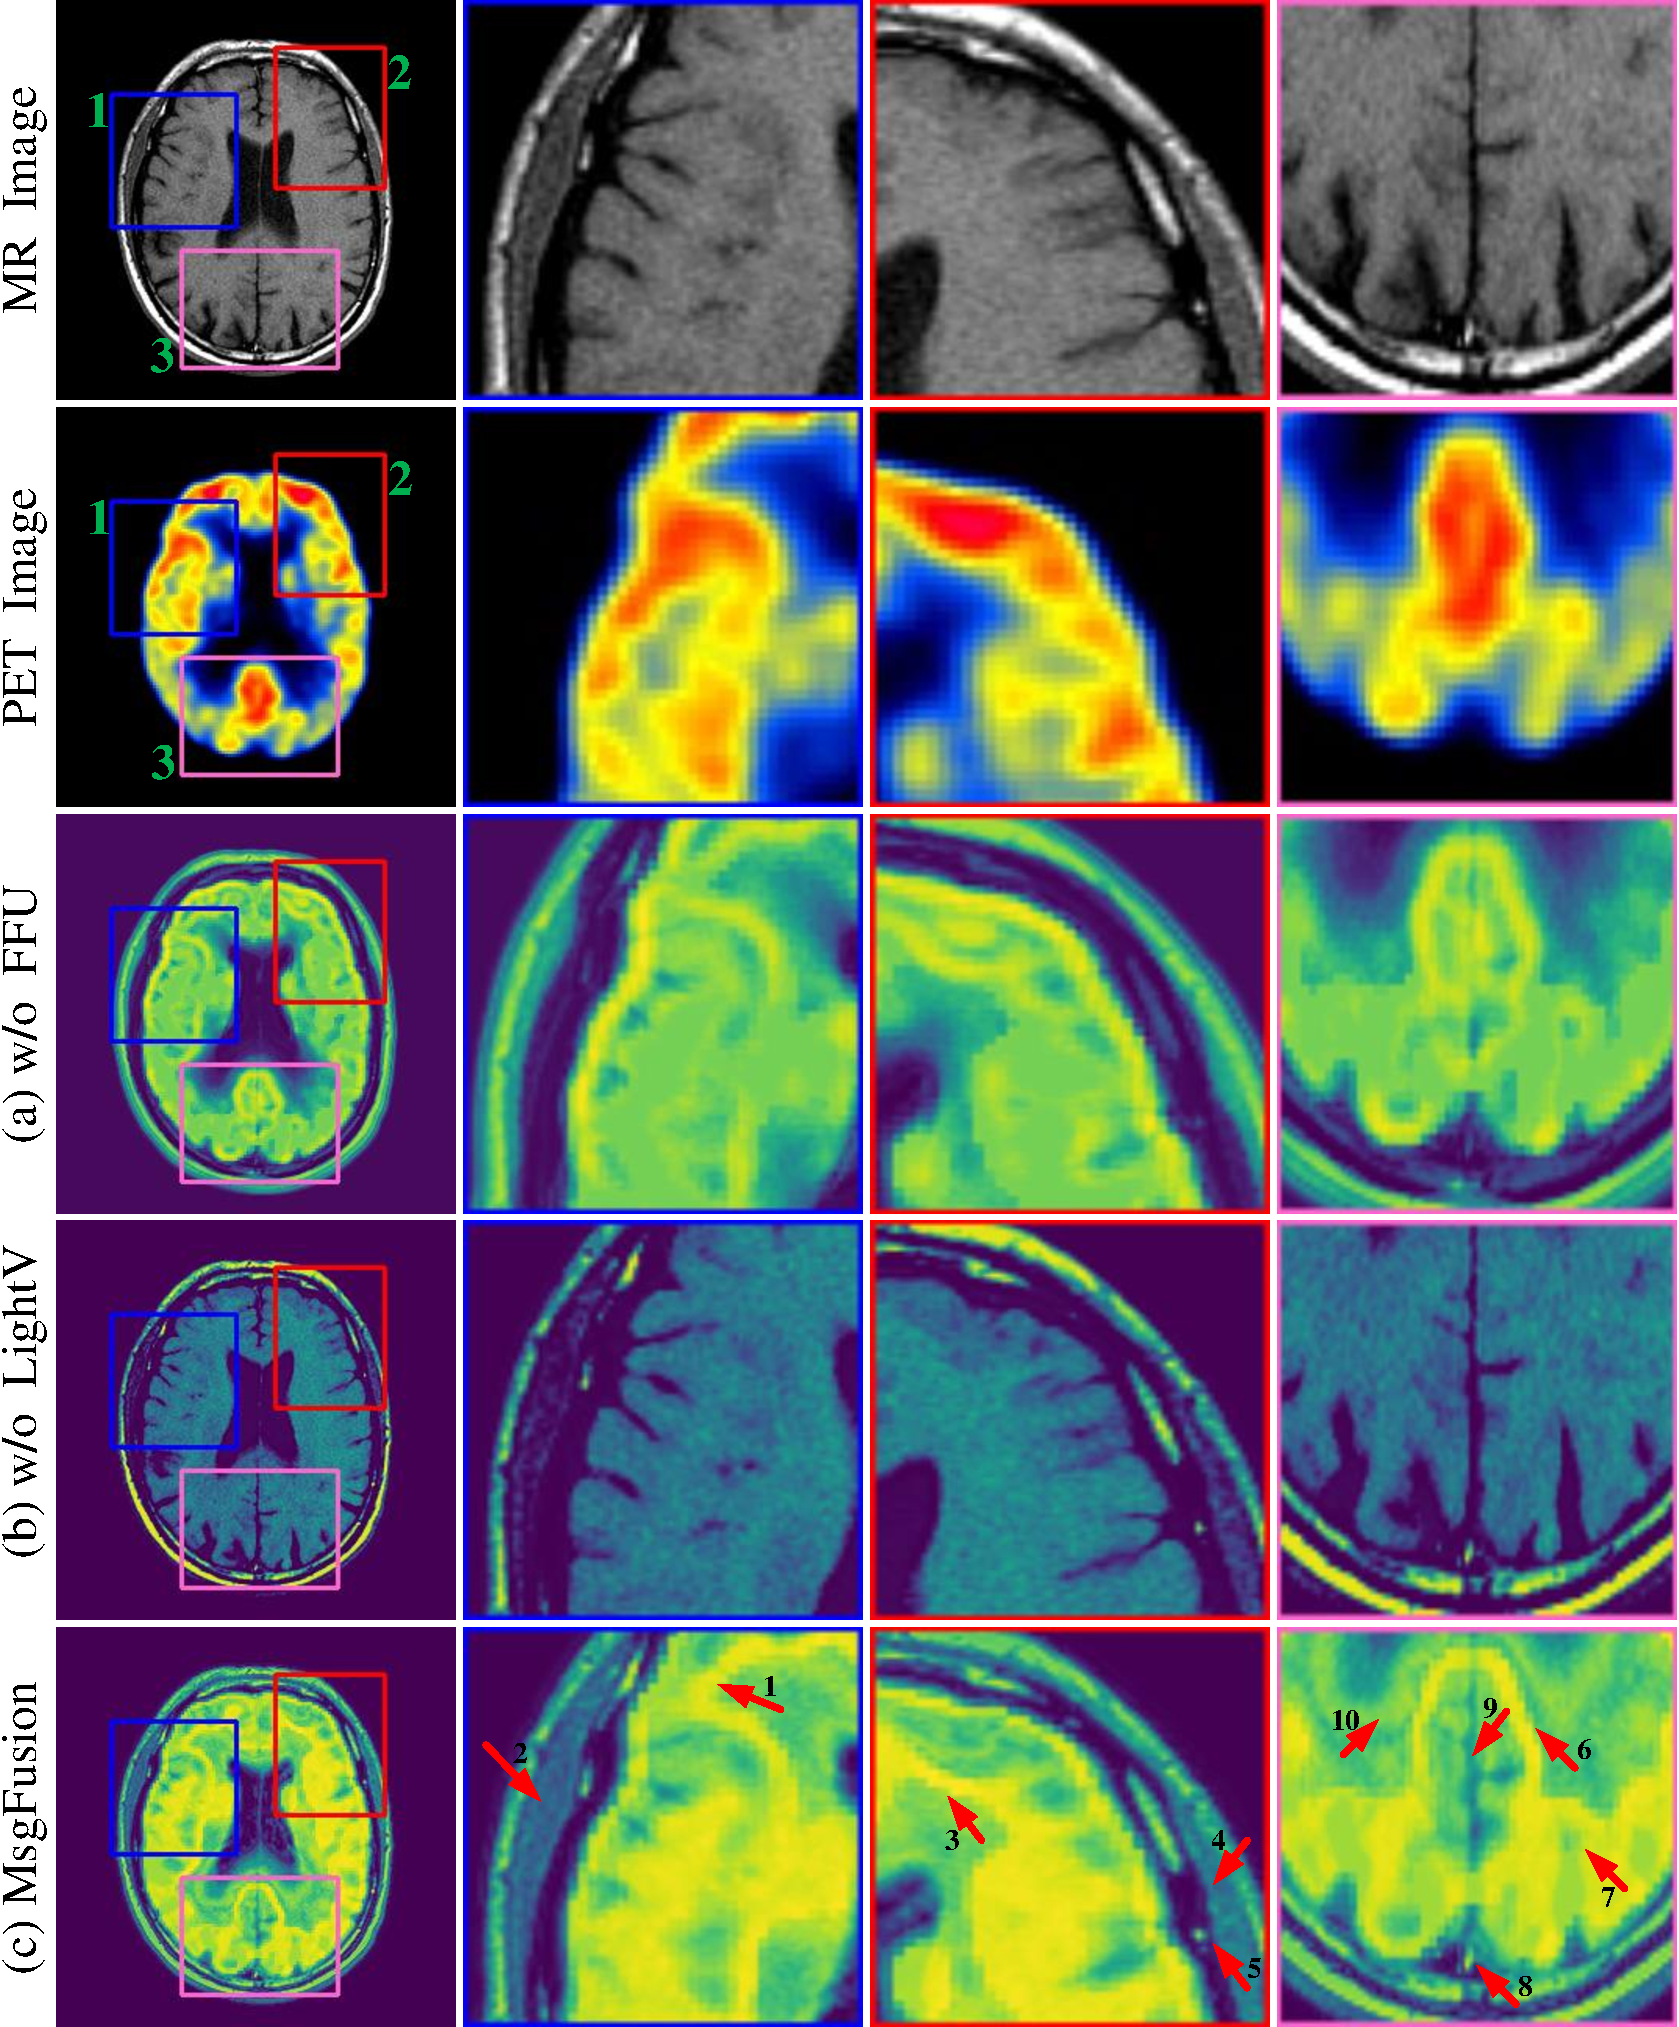
\includegraphics[width=0.8\columnwidth]{figs/paper1noHSVnoFourier_MAD015.pdf}
          \caption{本节所提出的影像融合方法的消融实验}\label{paper1noHSVnoFourier}
     \end{figure*}
     
\subsubsection{影像融合的消融实验}
为了说明在SF-Branch中结合频域和在GV-Branch中结合HSV颜色空间的必要性和有效性,本节对MRI-PET融合进行了消融实验。实验结果如图\ref{paper1noHSVnoFourier}所示。前两行显示MRI和PET的源影像及其各自的三个局部放大的ROI。下面的三行分别显示的是:(a)缺少频域处理,(b)缺少来自HSV颜色空间的改进亮度分量,(c)本节提出的MsgFusion方法。在最后一行局部放大影像中,标记了十个箭头,指向具有明显医学特征信息的区域。箭头1和3指向额叶,箭头2指向的是额骨,箭头4指向的是额骨内面,箭头5指向的是额骨和额叶之间的空间,顶叶区域由箭头6、7和10指示,箭头8指向的是上级矢状窦,并且箭头9指向大脑纵隔。当融合过程中不涉及FFT时,融合结果可以更完整地保留PET中的结构特征,但会丢失更多的MRI信息。当只使用FFT而不考虑HSV颜色空间的改进$V'$分量时,融合结果能较好地保留MRI的完整特征,但不能反映PET的功能信息。如图\ref{paper1noHSVnoFourier}的第五行所示,当同时考虑两者时,融合结果明显变得更好。

     
\begin{table*}[ht]
    \centering
  \caption{图\ref{paper1noHSVnoFourier}中对应的三种融合策略的质量评估}\label{paper1AblationIndex}
\begin{tabular}{ccccccc}
\hline
\textbf{Whole image}  &  EN         &  SD         &  MI         &  rSFe   &  SM         &  VIF  \\ \hline
w/o FFU                   &  \textcolor{red}{ 4.5027}      &  \textcolor{blue}{ 56.8141}     &  \textcolor{red}{ 9.0054}      & -0.5018                        & 0.2704                             &  \textcolor{blue}{ 0.3219} \\ 
w/o LightV                & 3.5768                             & 36.7745                            & 7.1537                             &  \textcolor{red}{ -0.2977} &  \textcolor{red}{ 0.3523}      & 0.1262                        \\ 
MsgFusion             &  \textcolor{blue}{ 4.476}       &  \textcolor{red}{ 67.5634}     &  \textcolor{blue}{ 8.952}       &  \textcolor{blue}{ -0.4103} &  \textcolor{blue}{ 0.3205}      &  \textcolor{red}{ 0.4076} \\ \hline
\textbf{Average ROIs} &  EN         &  SD         &  MI         &  rSFe   &  SM         &  VIF  \\ \hline
w/o FFU                   & 6.9201                        & 52.0514                        & 13.8401                        & -0.4204                   & 0.5594                             & 0.3227                   \\ 
w/o LightV                & 5.9916                             & 34.0278                        & 11.9832                            & -0.3802                   &  \textcolor{red}{ 0.6118} & 0.1738                   \\ 
MsgFusion             &  \textcolor{red}{ 6.9598} &  \textcolor{red}{ 54.9381} &  \textcolor{red}{ 13.9195} &  \textcolor{red}{ -0.3467} &  \textcolor{blue}{ 0.5830} &  \textcolor{red}{ 0.3652} \\ \hline
\end{tabular}
\end{table*}

表\ref{paper1AblationIndex}示出了图\ref{paper1noHSVnoFourier}中的6个评价指标的相应计算结果。表中的红色值是最佳值,蓝色值是次佳值。计算了整幅融合影像的评价指标,结果表明,本文所提出的方法效果较好(最优方法有2个指标,次优方法有4个指标)。此外,本节还计算了图10所示的三个ROI区域的评价指标的平均值,如表\ref{paper1AblationIndex}的接下来的四行所示。从三个ROI区域的评价指标的平均值也可以发现,本文的方法优于其他两种方法(缺少傅立叶应用和缺少V分量计算)。

\subsection{小结}
在这一节中,介绍了一种MS-Info引导下的脑部疾病影像深度特征融合方法MsgFusion。本节分析了MRI/CT/PET/SPECT的关键MS-Info,以获取其对应的影像特征,从而找到最有效的提取策略。为此,设计了一个包括SF-Branch和GV-Branch的双分支网络。SF-Branch结合了空间域和频域信息,GV-Branch结合了HSV颜色空间的多尺度灰度影像和亮度。双网络机制成功地提高了CNN的泛化能力,充分体现了频域信息和颜色空间信息的重要性,保证了融合结果的有效性。对医学脑影像进行了处理和分析,包括MRI-CT影像融合、MRI-SPECT影像融合和MRI-PET影像融合。实验表明,与现有方法相比,该方法具有明显的优势。本节还请求临床医生通过问卷调查的方式对融合结果进行评估。统计数据也证明了所提出的MsgFusion达到了最好的融合效果。在未来将考虑扩展框架,将CT、MRI、PET、SPECT、DTI和两种或两种以上其他成像手段整合在一起,并将其应用于临床诊断。

\section{基于脑影像的多维特征自适应融合} \label{chapter3.2:MdAFuse}
%磁共振成像与正电子发射断层成像的融合,可以将生物解剖信息和生理代谢信息结合起来,对临床诊断和病变定位具有重要意义。基于脑磁共振和正电子发射断层扫描影像的多维特征的基础上,我们提出了一种新的自适应多维特征线性融合方法(MdAFuse)。首先,在特征提取阶段,构建三维特征提取模块,从源影像中提取粗、细和多尺度信息特征。其次,在融合阶段,建立多维特征的仿射映射函数,保持特征间几何关系不变,有效利用特征映射图的结构信息,达到更好的重建效果。此外,我们提出的方法中还含有关键特征可视化增强部分,旨在观察脑病变的动态生长,这可以促进脑肿瘤的早期诊断和治疗。大量的实验结果表明,我们的方法从视觉感知和客观的影像融合指数上优于现有的融合方法。
%我们已在GitHub上分享了该方法的源代码(https://github.com/22385wjy/MdAFuse)。

\subsection{引言}
医学成像在各种临床应用中发挥着重要作用。其中,MRI和PET为多种疾病提供了影像学依据,广泛应用于各种疾病的临床诊断,如脑良恶性肿瘤、抑郁症、早发性AD、脑缺血等。MRI和PET脑影像的融合已被证明具有临床意义\cite{nakamoto2009clinical,heiss2009potential}。各种脑部疾病的诊断通常依赖于MRI-PET成像。脑病变的动态观察和脑肿瘤的定性分析也非常重要\cite{2019Inter}。MRI技术是通过捕捉人体内的电磁信号以实现成像的一种手段;该技术能清晰显示软组织,空间分辨率高,有利于病变范围的确定。PET扫描能够揭示人体内在的详尽生理活动和代谢状态信息,并且尽管空间分辨率低,但能显示人体组织中病变的异常变化。因此,MRI和PET的融合可以联合解剖结构信息和生理代谢信息,帮助医务人员更好地诊断脑部异常。MRI与PET结合的广泛需求也促使了一体化MRI-PET成像设备的发展(混合PET/MRI),但仍存在几个问题:PET和MRI系统相互干扰,购买和维护成本高,采集后的融合方法对设备性能至关重要,而目前应用于混合PET/MRI的融合方法多为传统方法,存在诸多局限性。因此,通过从不同设备开发更好的MRI和PET融合算法以及提高混合PET/MRI的性能来开发更有效的MRI-PET融合方法是重要的。由于不同模态的医学影像各自具有独特的特征属性,MRI-PET影像的融合具有挑战性:1.尽可能保留和增强MRI和PET的关键信息。2.选择适当的客观评价指标具有挑战性。3.在融合任务中,缺少真实对照组,因此损失层的正确选择变得至关重要。

目前,用于MRI-PET医学影像融合的传统方法有简单加权\cite{2018Infrared}、多分辨率金字塔\cite{2014Quantum}、小波变换\cite{2019Waveatom}、颜色空间\cite{2020An}、主成分分析\cite{2018Improved}、人类视觉系统\cite{2017Multifocus}等。近年来,深度学习已成为影像融合的代表性方法和研究热点。各种基于深度学习的影像融合方法相继被提出\cite{2018Deep,Zhong2016Image,liu2019medical}。利用深度学习进行影像融合是一种有效的解决方案,为了追求更好的感知效果,影像融合模型的设计主要是基于一些复杂的设计规则的定义来增强变换和融合策略。本小节提出了一种基于无监督深度学习的MRI-PET医学影像融合新思路。首先建立三维特征提取模块,提取源影像的浅层、深层和多尺度特征,然后建立多维特征的仿射映射函数,融合多维特征。本节工作可以总结为以下三个主要贡献:
\begin{itemize}
    \item 影像的多维分析分为三个模块,分别从源影像中提取浅层特征、深层特征和多尺度特征。这三个模块分别针对源影像中不同信息的重要性,尝试提取不同层次的特征,减少特征传递过程中的特征损失,提高后续特征融合的准确性。
    \item 建立仿射映射变换函数以保持不同维度特征之间的几何关系,并通过学习自适应地生成相关系数。从而在融合后的影像中充分保留MRI影像的空间纹理信息和PET影像的功能代谢信息等多维特征。
    \item 为了进一步增强融合影像的可视化效果,本文提出了一种基于能量的颜色增强算法,主要是增强融合影像中来自原始PET影像的能量信息。当用它来显示同一病例不同时间序列的异常区域时,病变的演变过程(例如,脑肿瘤)可以更好地追踪。
\end{itemize}


\subsection{相关工作}
目前,可应用于MRI-PET医学影像的融合方法包括一些传统的融合方法和基于深度学习(DL-based)的融合方法,每种类型都有自己的优缺点。在本节中,将讨论一些代表性的方法。

1)传统融合方法:在传统的影像融合方法中,简单加权平均法、小波变换应用和颜色空间交换是三种具有代表性的像素级融合方法,常应用于医学影像融合。Li等人\cite{2018Infrared}提出了一种基于潜在低秩表示(LatLrr)的简单有效的影像融合方法,旨在最大程度地保持原始影像中的有价值信息。该方法采用一种简单的加权平均融合策略。利用低秩聚类的思想,将影像分为低秩部分和重要部分,并将低秩部分和重要部分的加权和作为融合结果。LatLrr能突出影像的全局结构信息,但局部结构保持能力和细节提取能力较差。Hla等人\cite{2020Noise}将低秩分解方法用于含噪影像融合,主要通过最小秩正则化得到融合结果。

小波变换也是一种经典的方法。小波不仅具有正交性、双正交性和紧性,而且具有多分辨特性。Zhan等人\cite{zhan2015multifocus}提出了一种基于相位一致性融合(PCF)的影像融合方法;他们使用相位一致性来提取影像中的局部和剧烈变化。该方法在空间上使用Gabor小波滤波器来改善相位一致性。小波变换的应用\cite{2018ImageWen,2019Waveatom}也有利于理解影像,特别是医学影像。小波变换具有多分辨率的特点,可以从粗到细观察信号,但小波变换方法需要一个合适的母小波和一个可行的分解层次。为了便于医生理解影像,特别是观察PET影像中描绘的生理代谢变化,一些研究人员已经开发了融合策略来保持伪彩色。Du等人\cite{2020An}使用双尺度策略和色域变换来保持伪彩色信息,从而整合灰度影像(如MRI)和伪彩色影像(如PET和SPECT),并专注于保留伪彩色信息。然而,颜色空间转换也会造成一些信息损失。综上所述,一些传统的融合方法可以达到高质量的融合效果,但大多数融合方法依赖于人工对特定影像类型的特征提取规则,包括参数设置。随着影像类型和数量的增加,特征提取变得越来越复杂。同时,传统方法的泛化能力很弱。

2)基于DL的融合方法:在多模态影像融合中,将传统的技术手段与深度学习策略相融合,可以提高模型性能。Zhong等人\cite{Zhong2016Image}提出了一种基于CNN的联合影像融合和超分辨率方法。Rajalingam等人\cite{2020Intelligent}提出了一种深度引导混合多模医学影像融合(HMMIF)方法,该方法已应用于神经囊虫病(一种退行性疾病)的神经病理学。经典的传统方法和深度学习方法的结合可以有效地提高网络的性能。然而,一些传统的方法需要先验知识,并结合传统的方法可能会增加时间和空间复杂度。最近,一些端到端的深度神经网络已经应用于医学影像融合\cite{2019MCFNet, 2020Identification}。Rajalingam等人\cite{2018Multimodal}提出的新的医学影像融合方法使用了联合卷积神经网络来生成加权图,以融合来自多模态医学影像的像素运动信息。Zhao等人\cite{xiao2020global}提出了一种基于表示学习的通用融合框架,该框架研究的是基于边缘细节和对比度的特定领域的无参考感知度量损失,以优化学习过程,使融合影像呈现出更具体的表现。

为了加强U-Net在捕捉全局特征上的能力,Xiao等研究者\cite{xiao2020global}设计了两个单元(特征提取单元(GFPE)和注意力联合单元(GACU)),旨在高效地捕获并利用影像中的全局语义和边缘特性。无监督深度神经网络模型,如DeepVTF\cite{2019Deep}和VIFNet\cite{2020VIF}也被提出。DeepVTF方法在输入常规真彩色和融合输出之间建立视觉相似性度量,以获得自然直观的影像。VIFNet是定义了一个强大的混合损失函数,它是由一个修改的结构相似性度量和总变分组成。Nishant等人\cite{kumar2019structural}提出了一种名为FunFuseAn的深度神经网络模型,该模型使用SSIM作为损失函数来融合MRI和PET影像。Xu等人\cite{Xu2020A}介绍了一种基于梯度和连通域多焦点影像的深度融合模型。为了克服深度网络应用于多聚焦影像融合时梯度丢失的障碍,设计了一种掩模网络直接生成二值掩模。采用一致性验证策略,通过调整初始二值模板生成融合结果。Yu等人\cite{2020IFCNN}提出了融合模型IFCNN,它使用了迁移学习技术和最大张量策略。Xu等人\cite{2020FusionDN}介绍了一种无监督和统一的密集连接网络,称为FusionDN,用于不同类型的影像融合任务。该方法基于源影像的保留程度(即,源影像的质量和信息量)。

特别是近两年来,几种新的方法,如\cite{Zhao_2023_CVPR,XuTPAMI2022,LiangECCV2022}被提出。Zhao等人\cite{Zhao_2023_CVPR}提出了一种用于多模态影像融合的双分支变换器-CNN网络架构(CDDFuse)。为了提取特定的模态特征和模态共享特征,他们采用了Restormer、Lite Transformer和可逆神经网络模块。Xu等人\cite{XuTPAMI2022}构建了一种全新的端到端统一无监督影像融合架构(U2Fusion)。通过特征提取和信息测量,U2Fusion自动估计源影像中对应关系的重要性,并提供自适应信息保留。Liang等人\cite{LiangECCV2022}提出了一种强大的影像分解模型(DeFusion),它通过自监督表示学习来执行融合任务,而无需任何配对数据或复杂的损失函数。
深度学习方法的另一个重要分支是基于生成对抗网络(GAN)的方法\cite{xu2020mef,li2020attentionfgan}。受条件生成对抗网络(CGAN)的启发,Ma等人\cite{2019FusionGAN}将GAN引入影像融合和无监督GAN网络影像融合框架FusionGAN。

与传统方法相比,深度学习方法具有自主学习、灵活的实时处理和良好的泛化性能的特点。在基于深度学习的方法中已经发现了相当大的潜力。但目前,专门为医学影像融合设计的深度神经网络仍处于初期。可应用于混合PET/MRI的相应方法更是罕见。在这小节中,专注于从MRI和PET影像中提取和保留关键特征。为了实现这一目标,设计了多维特征模型和自适应线性融合策略。
        
\subsection{多维特征自适应线性融合网络}
如图\ref{paper2flowchart}所示,本文的工作包括两个方面。首先,本节提出了一个基于多维特征自适应线性融合的MRI和PET脑影像融合网络(adaptive linear
fusion method for multi-dimensional features,MdAFuse)。其次,本节提出了一种基于能量的可视化方法,以进一步增强融合影像。在融合网络中,本节采用了多维特征提取方法和自适应线性融合策略,这两方面将分别在\ref{chapter3.2:Feature_extraction}小节和\ref{chapter3.2:Fusion_strategy}小节中详细介绍。\ref{chapter3.2:Loss_function}小节将解释如何设置该网络的损失函数。随后,将在小节\ref{chapter3.2:Enhancement_of_key_features}中描述所提出的可视化方法。
    
\begin{figure*}[ht]
      \centering
      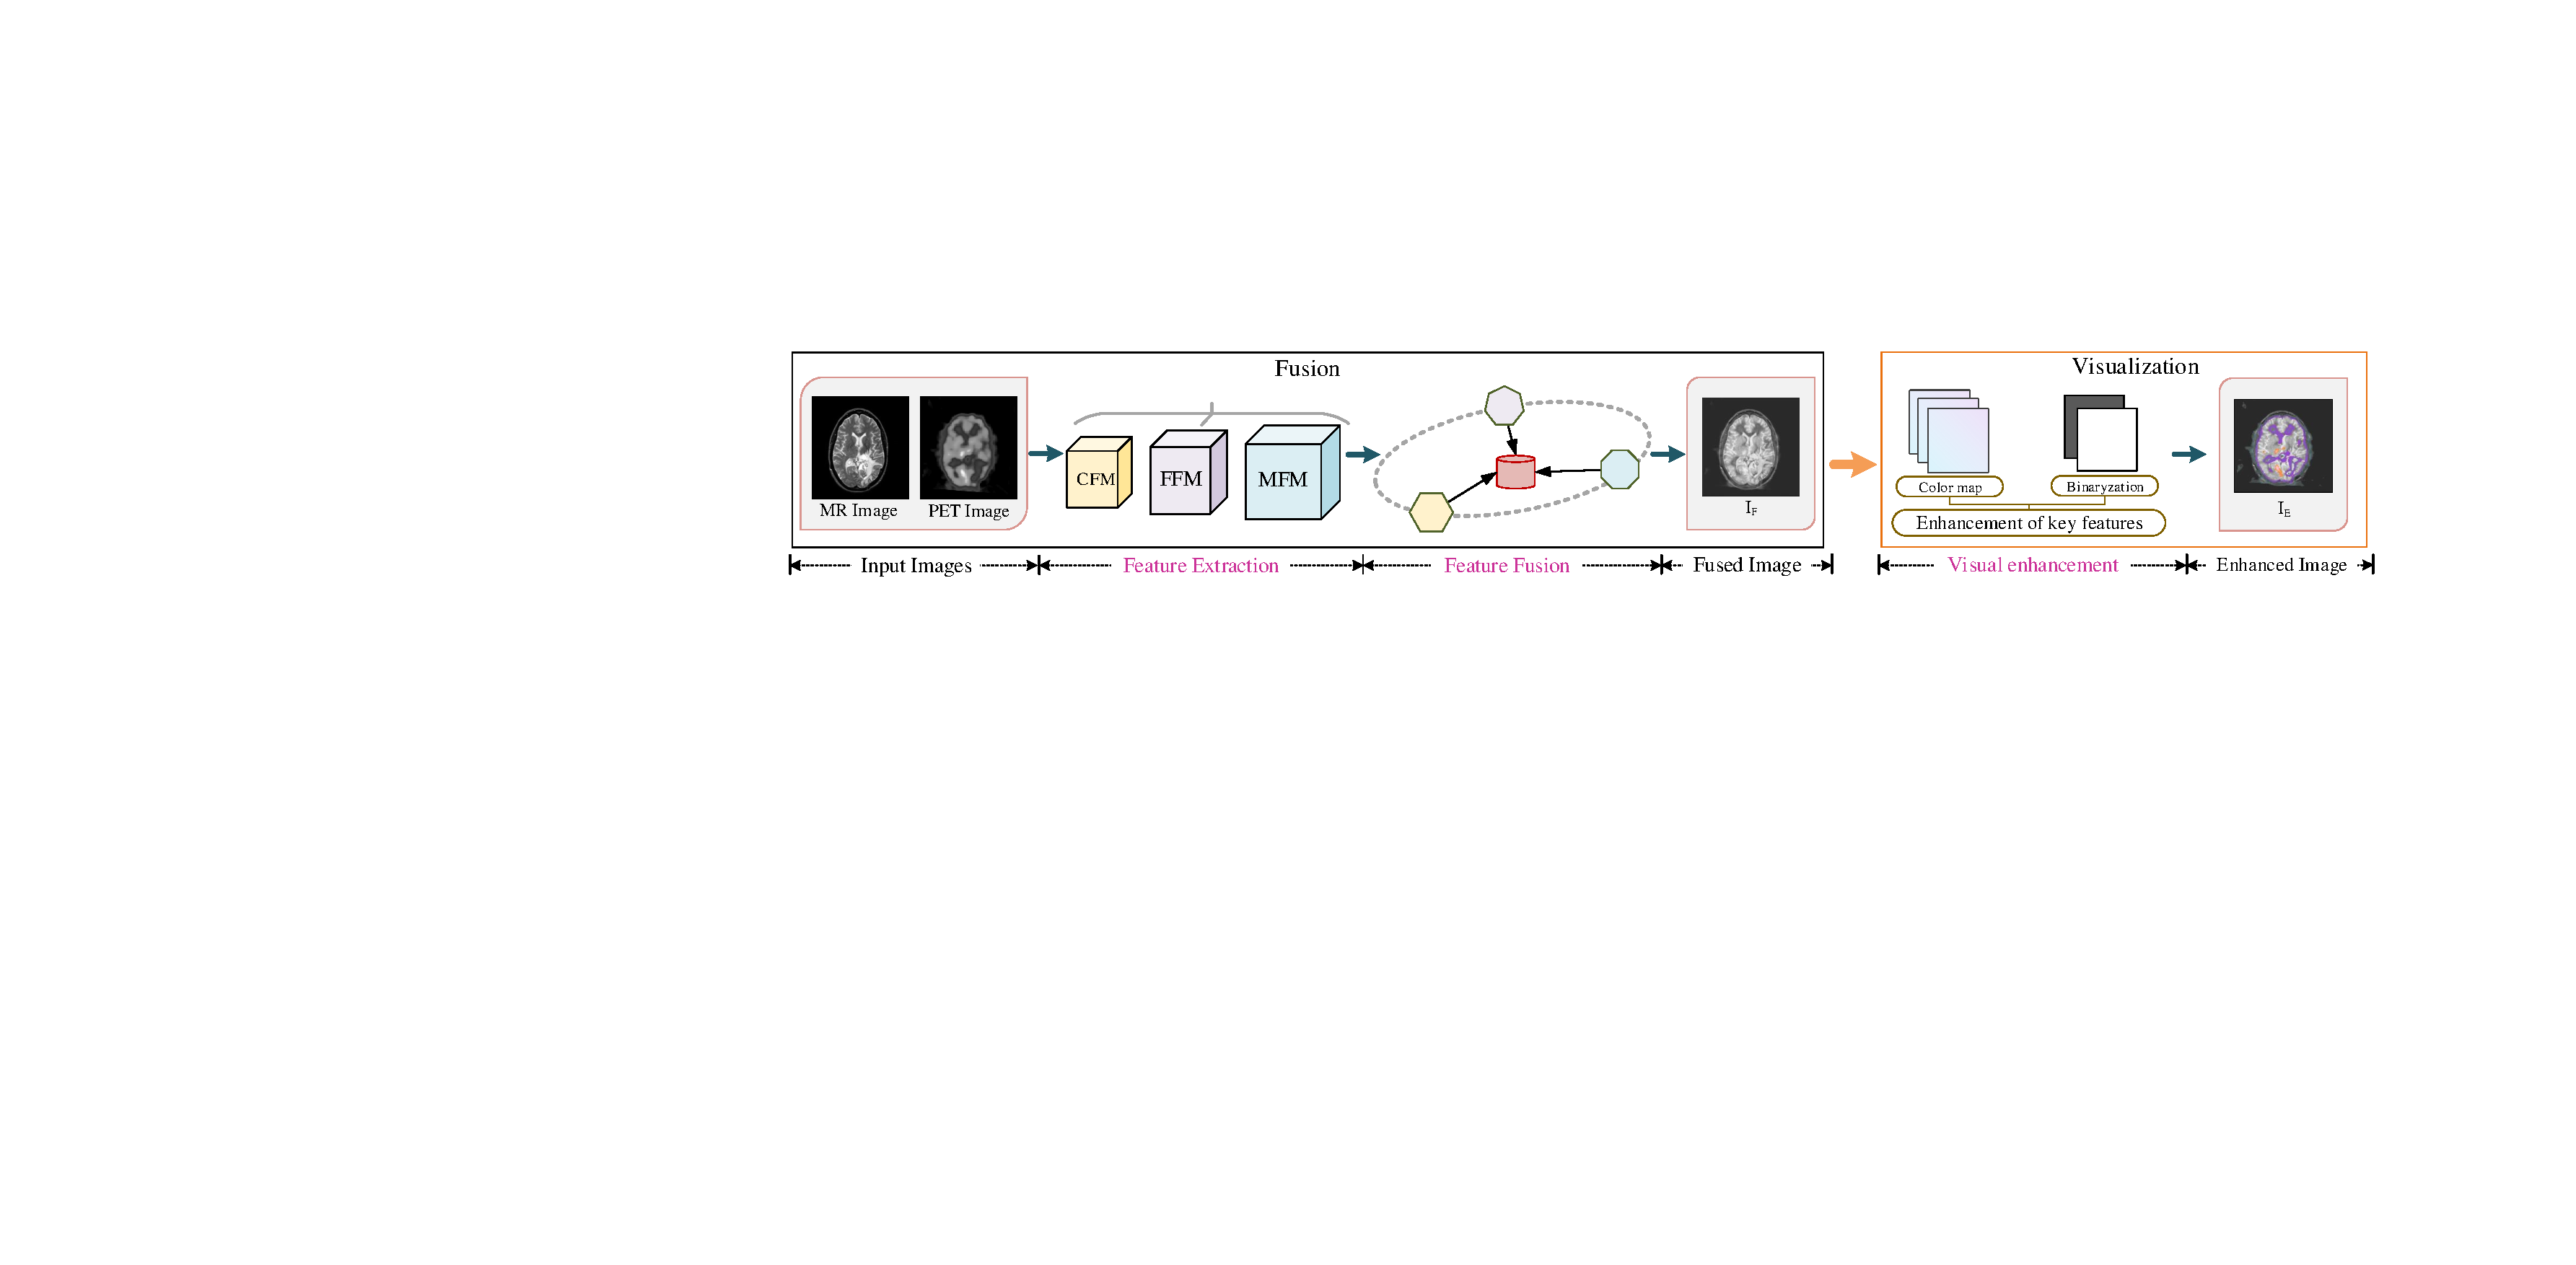
\includegraphics[width=0.97\linewidth]{figs/paper2Outline20230723.pdf}
      \caption{本小节提出的方法流程图(包括两个阶段:影像融合(图\ref{paper2framework})和可视化增强(图\ref{paper2visualization}))}\label{paper2flowchart}
    \end{figure*}

\subsubsection{多维度特征的提取策略}\label{chapter3.2:Feature_extraction}
为了从源影像中提取尽可能多的特征,本节采用多维度策略,充分利用空间和通道特征,建立了浅层特征模块(coarse feature module,CFM),深层特征模块(coarse feature module,FFM)以及多尺度特征模块(multi-scale feature module,MFM),分别提取浅层特征信息、深层特征信息以及多尺度特征信息。图\ref{paper2framework}中的蓝色虚线矩形表示特定的特征提取过程。其中,CFM为紫红色实线边缘黄底区域,FFM为蓝色实线边缘紫底区域,MFM为紫色边缘蓝底区域。在图\ref{paper2framework}中,不同的小方块代表三个步骤的组合(卷积运算,批量归一化和ReLU激活),不同颜色的方块代表不同大小的卷积核,黄色是1,蓝色是3,绿色是5,紫色是7,粉红色是3。不同大小的正方形表示不同的特征图大小和输出通道数。图\ref{paper2framework}右下角的灰色虚线框中有不同通道号的定义,即不同宽度的长方形代表不同通道的输出数量,并且颜色越深,通道的数量越大。对于输入影像,特征提取模块将获得三个维度的特征,即$CF_1$、$FF_1$和$MF_1$。 这些特征提取模块是根据人类视觉感知的感知特性和影像的物理特性设计的。

在图\ref{paper2framework}中,CFM由紫红色实线包围的黄色背景区域表示。CFM代表浅层特征模块,它负责通过卷积运算从影像中提取浅层特征。该模块利用较大的卷积核和较小的特征通道来捕捉影像的主要形状结构和边缘轮廓信息,代表影像背景和物体轮廓等全局低频信息。从图\ref{paper2framework}所示的特征图中,可以观察到,CFM模块提取的CF特征图表现出更清晰的轮廓。
类似地,在图\ref{paper2framework}中,FFM由蓝色实线包围的紫色背景区域表示。FFM指的是深层特征模块,它专注于深层特征提取。该模块采用较小的卷积核和较大的特征通道来捕获纹理细节,例如边缘,精细纹理细节和噪声,表示影像内具有显著变化的局部高频信息。用于深层特征提取的通道数远大于用于浅层特征提取的通道数。从图\ref{paper2framework}所示的特征图中,可以观察到由FFM模块提取的FF特征图显示了更明显的纹理细节。

在图\ref{paper2framework}中,MFM是紫色包围的蓝色背景的区域。MFM主要是从金字塔和分类的思想中获取影像的空间结构,从而获得多尺度影像之间的互补信息,利用多分辨率和多尺度影像之间的互补信息实现精细融合。在MFM中,还使用了深度分离卷积网络,便于挖掘更丰富有用的信息,为后续的影像理解和应用分析提供了良好的基础。另外,本节在构建网络时使用跳跃连接方法,与参考文献\cite{he2016deep,huang2017densely}一样。在本节的特征提取模块的设计中,更强调局部细粒度的信息,而不仅是全局特征。因此,使用短跳跃连接有利于局部信息的传输和保存,使网络能够更好地学习和利用这些局部化特征。因此,在特征提取过程中采用了短跳级联的方法,以获得更详细的信息,实现特征的逐步融合。

    \begin{figure*}[htbp]
      \centering
      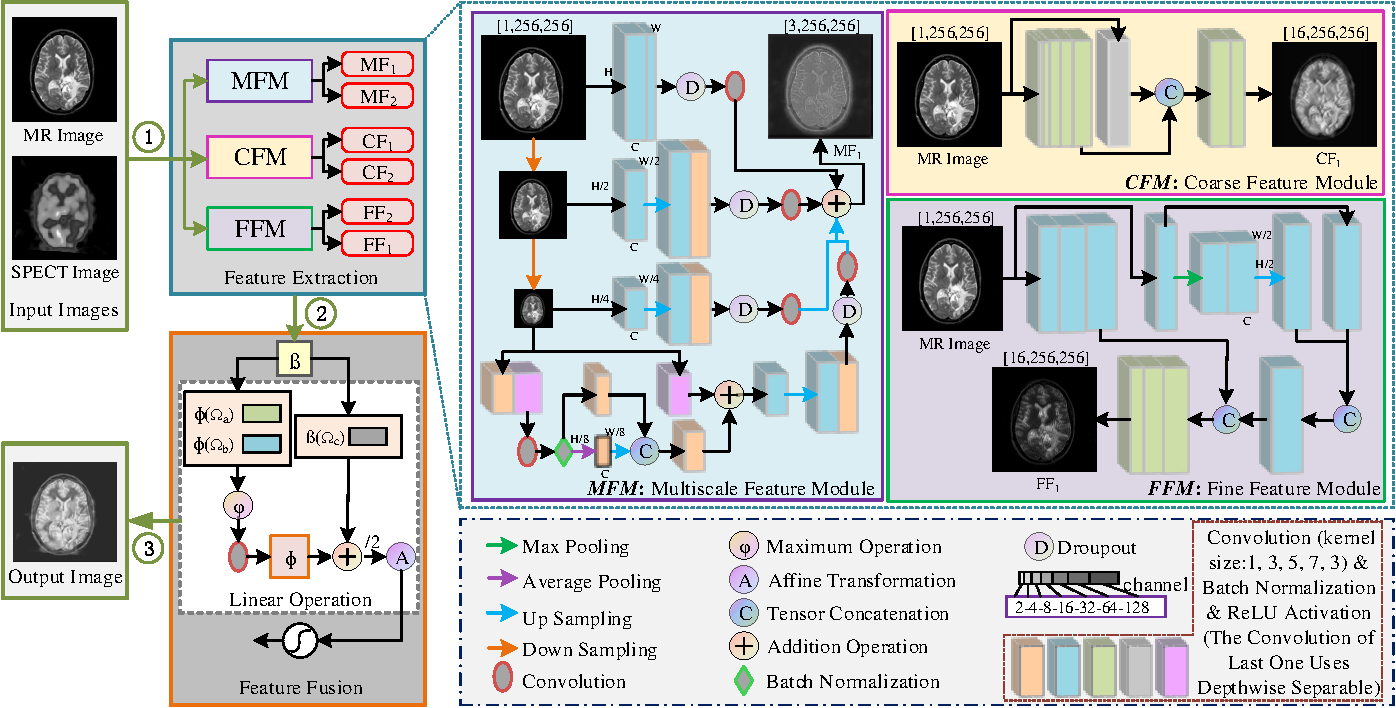
\includegraphics[width=0.9\linewidth]{figs/paper2framework.pdf}
      \caption{多模态影像融合网络的框架及具体的实现步骤}\label{paper2framework}
    \end{figure*}
\subsubsection{多维度特征的融合策略}\label{chapter3.2:Fusion_strategy}
MdAFuse从三个维度提取特征。浅层特征主要体现在边缘轮廓信息上,而深层特征则能保留纹理细节。为了从一幅影像中同时获得高频信息和低频信息,将每幅影像的粗特征和细特征相加,以获得具有更多信息的影像特征。为了突出两幅影像中的显著特征,特别是PET影像上的突出信息(通常对应于异常区域),本节使用最大值来获得更突出的部分。多尺度特征可以提供更多的结构信息,也可以补偿在跨尺度上丢失的局部细节。因此,浅层和深层特征必须是多尺度的。对于每个输入,将获得三个特征(CF、FF和MF)。那么,当输入两个模态影像时,共提取六个特征。并提出了一种自适应融合策略,使融合结果同时包含6个特征。本节设计的目标函数如(\ref{paper2tofuse}):
\begin{equation}\label{paper2tofuse}
   F=\delta(\Phi( (\upsilon (\varphi(\Phi(\Omega_a),~ \Phi(\Omega_b)) ) +\beta(\Omega_c))/2 )),
 \end{equation}
其中,$F$是融合的结果。 $\delta$ 是激活函数,本文采用$tanh$。$\Omega_a = \{ CF_1 \} \cup \{ FF_1 \}$, $\Omega_b = \{ CF_2 \} \cup \{ FF_2 \}$, $\Omega_c$ = $(MF_1+MF_2)/2$. 当计算$\Omega_a$的$\Phi$ 时,$\Gamma_1$和$\Gamma_2$分别表示$CF_1$和$FF_1$特征。类似地,如果计算$\Omega_b$的$\Phi$,$\Gamma_1$和 $\Gamma_2$分别表示$CF_2$和$FF_2$特征。
$\Phi$是通过仿射变换获得的两个特征之和,如等式(\ref{paper2F1})。在这个等式中,$U$表示特征图的大小。$A=Diag(B)$, $\beta(\Gamma)= A\Gamma(i)+e$, $B$和$e$是可学习参数。设置大小的规则与后归一化的规则相同\cite{2021Going}。 初始化$B$的值为1,$e$为0。 $\beta$是仿射变换函数,用于表示特征之间的相关性。在几何学领域,仿射变换被描述为一种结合了非奇异线性映射与平移的变换过程,它连接了两个向量空间并保持了它们的仿射结构,可用于保持二维影像之间的位置关系。因此,仿射变换被用作融合特征,以充分利用特征之间的相关性并保持它们。
 \begin{equation}\label{paper2F1}
\Phi(\Gamma)=\beta(\sum_{i=1}^{U}\Gamma_1(i))+\beta(\sum_{i=1}^{U}\Gamma_2(i))=A\sum_{j=1}^{2}\sum_{i=1}^{U}\Gamma_j(i)+2e,
 \end{equation}

$\upsilon$表示卷积运算,以保持输入和输出维度一致。$\varphi$是取最大值操作为突出显示重要信息。



\subsubsection{损失函数的构建}\label{chapter3.2:Loss_function}
为了更准确地重建源影像,在训练阶段考虑了特征提取阶段和融合过程,并获得了最小损失函数如式(\ref{paper2loss_function}):

 \begin{equation}\label{paper2loss_function}
   L=\alpha L_S +\beta L_M
   %L=L_S + L_M
 \end{equation}

同\ref{chapter3.1:MsgFusion}小节中的损失函数(\ref{paper1loss_function})设计相同,总损失函数由结构相似度$L_{S}$和像素损失$L_{M}$组成,具体计算同式(\ref{paper1L_{SSIM}})和(\ref{paper1L_{P}}):


在等式(\ref{paper2loss_function})中,$\alpha$和$\beta $是设置在区间$[0,1]$中的权重参数。通过对比分析,我将$\alpha $设为0.3,$\beta $设为0.7,结果最佳。在训练过程中,初始学习率为0.0001,60 epoch,批量大小为2,采用批量归一化,优化函数为Adam。

    \begin{figure*}[htbp]
      \centering
      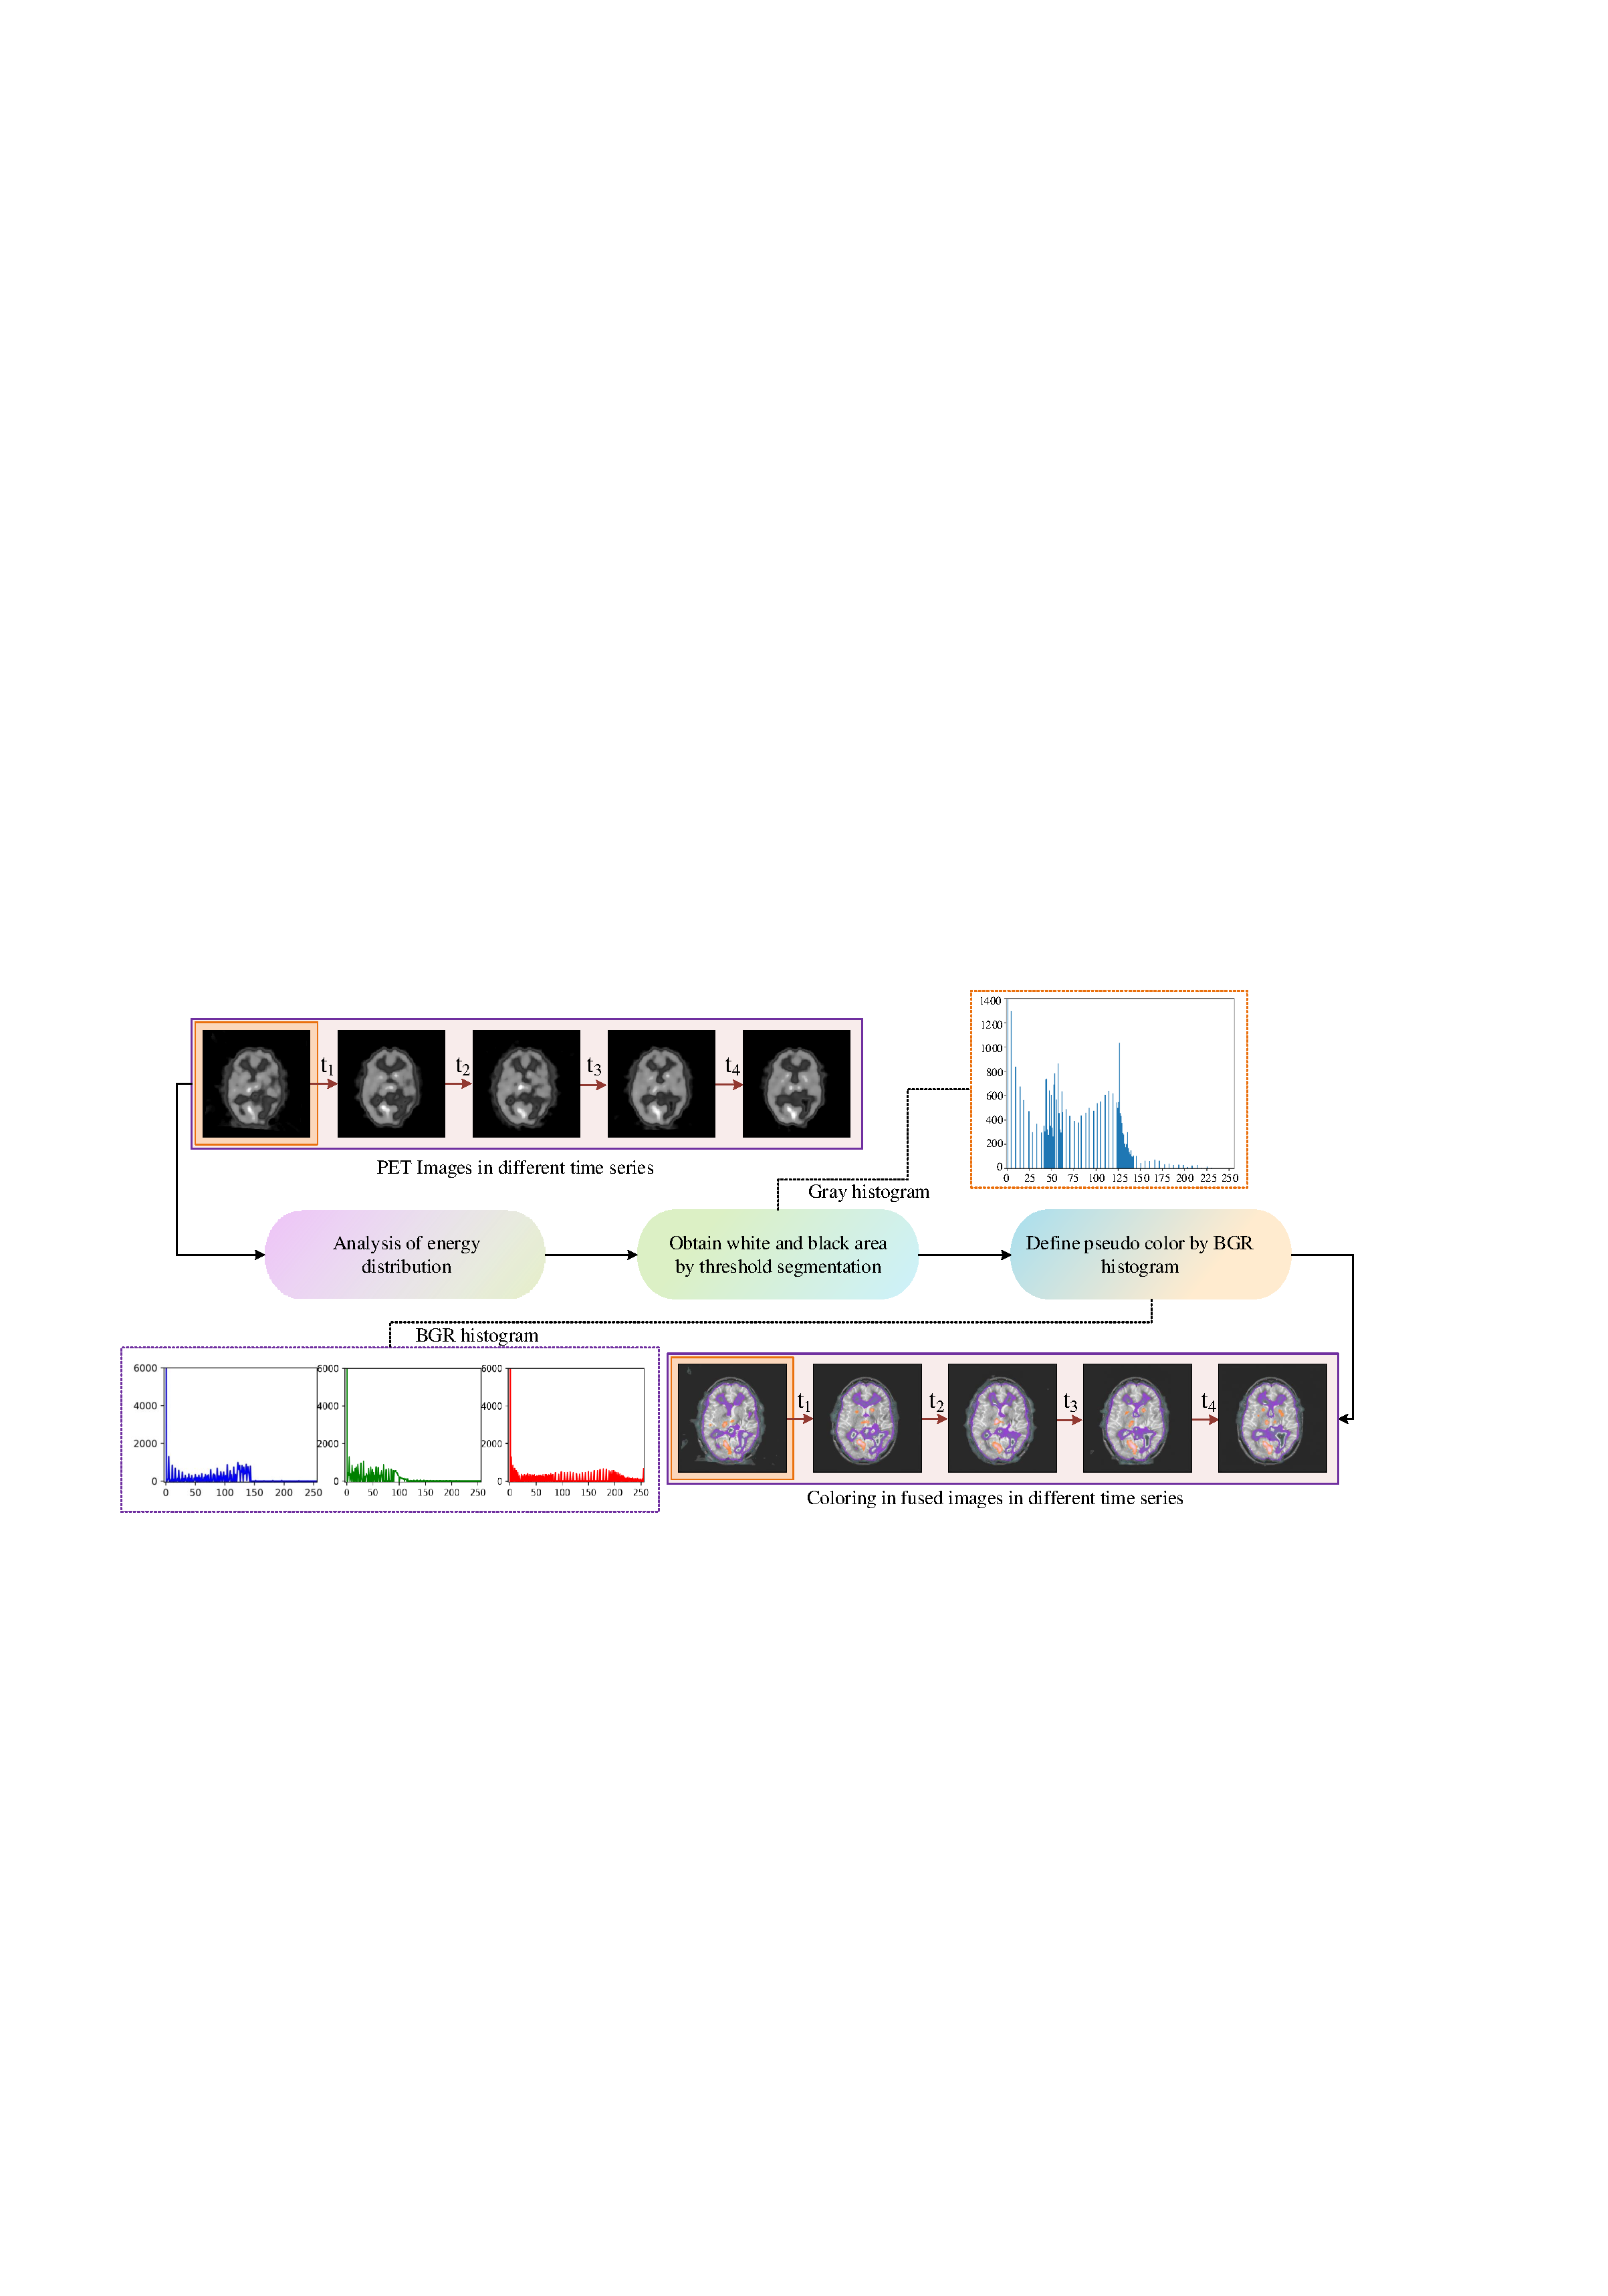
\includegraphics[width=0.9\linewidth]{figs/paper2visualization2023.pdf}
      \caption{增强融合影像中的关键特征策略}\label{paper2visualization}
    \end{figure*}
    
\subsubsection{关键特征的增强方案}\label{chapter3.2:Enhancement_of_key_features}
PET或SPECT影像的空间分辨率有限,边界灰度区分不清,限制了异常和正常区域的区分。为了提高可视性,伪彩色处理通常应用于临床环境,帮助医生识别边界细节并提高疾病诊断的准确性。


\begin{algorithm}[htbp]
\caption{Energy-based color enhancement}\label{paper2enhanceAlgorithm}
\centering
\begin{algorithmic}  [1]
    \Require Images $I_g$, $I_f$  
    \Ensure Image $I_e$
    
    \State $x \leftarrow $ the weight of $I_g$
    \State $y \leftarrow $ the height of $I_g$
    \State $\rho_w \leftarrow$ self-defined color for image of white area
    \State $\rho_b \leftarrow$ self-defined color for image of black area 
    \State $\eta_w,~ \eta_b \leftarrow$ $\gamma(I_g)$  %BinaryImage
    \State $\sigma \leftarrow$ \Call{\text{ColorUp}}{$I_g,~I_f,~ \eta_w,~ \rho_w$}
    \State $I_e \leftarrow$ \Call{\text{ColorUp}}{$I_g,~ \sigma,~ \eta_b,~ \rho_b$}
    %\State $I_e \leftarrow f_2$  
    %\State
    \end{algorithmic} 
    
\begin{algorithmic}[1]
\Function{ColorUp}{$I_g,~ I_f,~ I_a,~ I_c$}
   \State $I \leftarrow I_f.\text{copy}()$
        \If{$I_c == \rho_w$}
            \State $\quad \mu \leftarrow 5\sigma-20, ~\sigma=0,2,6,8$ %[-20,~ -10,~ 10,~ 20]
            \State $\quad \xi \leftarrow 5\iota-20,~0 \le \iota \le 4$
        \ElsIf{$I_c == \rho_b$}
            \State $\quad \mu \leftarrow 5\sigma-20,~0 \le \sigma \le 11 \&~\sigma\neq4$
            \State $\quad \xi \leftarrow 5\iota+10,~0 \le \iota \le 11$
         \EndIf
        \For{$i$=1 to $x$}
            \For{$j$=1 to $y$}
                \If{$I_a(i, ~j) \neq 0$}
                    \State $ a_{ij} \leftarrow I_a(i, ~j)$
                    \State $ \psi \leftarrow I_f(i, ~j) - I_g(i, ~j)$
                    \For{$k$=1 to  $(\text{len}(\mu))$}
                        \State $ I^{'}$  $\leftarrow I[a_{ij}]$
                        \State $ I_{c}^{'}$  $\leftarrow I_c[a_{ij}]$
                        \If{$\psi \leq \mu[k]$}
                            \State $\quad I^{'}(i, ~j) \leftarrow I_{c}^{'}(i, ~j) + \xi[k]$
                         \Else
                            \State $\quad I^{'}(i, ~j) \leftarrow I_{c}^{'}(i, ~j) + \xi[-1]$
                         \EndIf
                    \EndFor
                 \EndIf
            \EndFor
        \EndFor
      \State \Return $I^{'}$
\EndFunction
\end{algorithmic}
\end{algorithm}

在通过MRI-PET/SPECT融合生成灰度融合影像时,来自MRI的空间纹理是清晰的,而低分辨率灰度PET/SPECT影像难以揭示葡萄糖代谢的显著异常。现有的伪彩色方法涉及基于灰度的离散颜色映射和从灰度到颜色属性的连续转换。然而,这些技术中没有一种侧重于突出PET/SPECT影像中的这些显著异常。为了强调这些异常,基于PET/SPECT能量的灰度直方图,本节提出了一种颜色增强算法。该算法增强了异常信息的视觉效果,详细描述见算法\ref{paper2enhanceAlgorithm}和图\ref{paper2visualization}。


其中,$I_g$表示灰度PET/SPECT,$I_f$为融合的影像,$I_e$为增强的影像,$\eta_w$和$\eta_b$分别为阈值二值化过程中的白色和黑色区域。$\rho_w$和$\rho_b$是白色和黑色区域的两种自定义颜色。$I_c[a_{ij}](i,~j)$表示$I_c$中对应于$I_a$的区域。关键特征增强过程如图\ref{paper2visualization}所示。在这部分工作中,主要目的是获得可以代表葡萄糖含量或生理代谢的PET/SPECT影像和增强融合结果中的重要信息。


首先,分析灰度PET/SPECT影像中的能量分布,包括不同像素的大小分布、不同位置像素的分布、有用信息的集中区域以及代表相似信息的区域数量。在PET/SPECT中主要存在两种形式的能量分布。一种是葡萄糖含量高或代谢旺盛的组织,显示在白色区域。另一种是葡萄糖含量低或代谢弱的组织,用黑色区域表示。其次,需要在灰色PET/SPECT中获得黑色和白色区域。使用阈值法来提取这两种类型的影像。阈值化的关键在于阈值的设置,$\tau_w$是提取白色区域块的阈值,其由等式(\ref{paper2Tw})获得,$\zeta$是指直方图中峰值的灰度值,$\kappa$表示指峰的总数。在公式(\ref{paper2Pks})中的函数表示直方图的计算,$\phi$表示其转换到一维的操作。参数$\chi$表示峰与其周围谷之间的最小高度差,在图\ref{paper2visualization}的示例中设置为100。$\vartheta$的作用是寻找直方图中的峰值。对于黑色区域,设置了两个阈值。为了消除一些噪声并避免假溢出,添加另一个阈值$\tau_{b1}$,其被设置为10。$\tau_{b2}$是通过Otsu方法获得的全局阈值。算法1中的$\gamma$表示白色特征和黑色特征的两个二值影像,这两个二值影像是由公式(\ref{paper2Ia})和(\ref{paper2Ib})分别的计算获得。在式(\ref{paper2Ia})和(\ref{paper2Ib}),$I_{g}(i,~j)$表示影像$I_{g}$中第$i$行第$j$列的位置处的像素值。
 
\begin{equation}\label{paper2Pks}
\zeta =\vartheta\left(\chi\left( \phi \left(I_g\right)\right), ~p\right) ,
\end{equation}
\begin{equation}\label{paper2Tw}
%\tau_w =P_{k s}\left[N_{k s}-1\right] 
\tau_w =\zeta^{l},~ l=\kappa-1,
\end{equation}
\begin{equation}\label{paper2Ia}
\begin{aligned}
I_{w}(i,~ j)=\begin{cases}
0,  & I_{g}(i,~ j)\le \tau_w\\
255,  & I_{g}(i,~ j)>\tau_w\\
\end{cases} \\
\end{aligned},
\end{equation}
\begin{equation}\label{paper2Ib}
\begin{aligned}
I_{b}(i,~ j)=\begin{cases}
0,  & I_{g}(i,~ j)< \tau_{b1} ~\|~ I_{g}(i,~ j)>\tau_{b2}\\
255,  & I_{g}(i,~ j)>\tau_{b1} ~\&~ I_{g}(i,~ j)\le \tau_{b2}\\
\end{cases} \\
\end{aligned},
\end{equation}


最后,根据BGR直方图定义伪彩色,具体过程如算法2所示,在图\ref{paper2visualization}中包含三幅影像的直方图(根据伪彩色PET/SPECT影像计算的相应BGR的三种颜色的直方图)。为了便于观察,纵轴的值仅小于6000。从BGR直方图中,可以确定蓝色、绿色和红色像素值的大致范围。因此,白色区域呈现黄色显示,黑色区域呈现深蓝色显示。$\rho_w$和$\rho_b$分别用于表示黄色和深蓝色区域。亮度根据像素的大小而变化,并且对于没有辅助诊断的区域不显示颜色。然后,将融合影像与原始PET/SPECT灰度影像之间的像素值进行比较,并做出相应的改变。具体过程如算法\ref{paper2enhanceAlgorithm}的$ColorUp$所示,以及得到的影像的着色效果如图\ref{paper2visualization}所示。


\subsection{多模态影像融合的实验}
本节使用Python 3.7.9和Pytorch版本1.7.1+cu110及其相应的CUDA版本11.1。GNU/Linux x86,GeForce RTX 3090 Ti GPU 20GB RAM-64系统。在训练过程中,使用的数据来自ADNI(https://adni.loni.usc.edu/data-samples/access-data/),本节下载了555个MRI和PET影像对。样本的年龄从55岁到90岁不等,样本的性别有男有女。所有影像均作为轴向切片进行分析,体素尺寸为1.0$\times$1.0$\times$1.0 $mm^{3}$。通过非相交数据集测试对本节的训练模型进行交叉验证。
从ADNI和全脑图谱(http://www.med.harvard.edu/AANLIB/home.html.)中获得了80个独立不重复受试者的137个影像对进行测试。其中,74对MRI-SPECT,42对MRI-PET,21对MRI-CT。在图\ref{paper2d2roi}和图\ref{paper2029_1_roi}的融合实验中,测试数据是具有胶质瘤的MRI和SPECT脑影像,这是脑神经系统中的典型应用。MRI与PET/SPECT的融合可以整合生物解剖信息和生理代谢信息,帮助医生对病变进行定位和诊断。实验中还分析和比较了现有的几种基于传统方法和深度学习方法的融合算法。

为了定量衡量不同融合方法的融合效果,本节采用了9种质量评价指标,信息熵(EN)\cite{2008Assessment},互信息(MI)\cite{2005Feature},标准差(SD)\cite{Yun1997In},视觉信息保真度(VIF)\cite{2013A},结构相似性(SSIM)\cite{wang2004image},差异相关性之和(SCD)\cite{Aslantas2015A},相关系数(CC)\cite{han2008study},均方误差(MSE)\cite{willmott2005advantages}和空间频率误差比(rSFe)\cite{2007A}。对于MSE,较小的值表示更好的性能。对于rSFe,其较小绝对值对应于较好的融合效果。而其他七个评价指标则相反。rSFe是一个相对不常见的评价指标,用于衡量影像的整体活动水平,它由像素点中的四个空间频率(行、列、主对角线、次对角线)和四个方向的一阶梯度值(水平、垂直、主对角线、次对角线)整合而成,其数值绝对值越小,则表明融合效果越佳。为了便于比较和分析,本节对部分指标的计算结果进行了归一化处理。如表\ref{lineTransformation}所示,本节对每个度量执行线性变换,其中$k_i$和$b_i$ ($i=1, 2, 3$)分别表示图\ref{paper2d2_10roi_value}、图\ref{paper2029_1_roi_value}和图\ref{paper2ablation_value1}中的变换系数。

\begin{table}[ht]
%\small
\centering
  \caption{每个度量指标值上的线性变换,其中$k_i$和$b_i$ ($i=1, 2, 3$)分别表示图\ref{paper2d2_10roi_value}、图\ref{paper2029_1_roi_value}和图\ref{paper2ablation_value1}中的变换系数}\label{lineTransformation}
\begin{tabular}{cccccccccc}
\hline
\textit{\textbf{}} & \textbf{EN} & \textbf{MI} & \textbf{SD} & \textbf{VIF} & \textbf{SCD} & \textbf{SSIM} & \textbf{CC}  & \textbf{MSE} & \textbf{rSFe} \\ \hline
$k_1$                 & 8           & 6           & 1/2.1     & 48           & 29  & 16   & 42  & 18  & -37  \\
$b_1$                 & -11         & 0           & 0           & 0            & 2   & 0    & 5   & 5   & 8    \\
$k_2$                 & 5.6         & 5           & 0.4         & 31           & 18  & 16   & 26  & 240 & -32  \\
$b_2$                 & 0           & 0           & 0           & 0            & 0   & 0    & 0   & 3   & 6    \\
$k_3$                 & 1           & 1           & 1/13     & 5            & 2   & 10   & 100 & 15  & -8   \\
$b_3$                 & -1          & 0           & 0           & 0            & 0   & -14  & 90  & 0   & 0    \\
\hline
\end{tabular}
\end{table}

\subsubsection{与传统方法的实验对比分析}
在本小节测试了三种传统的融合方法,并将它们与本节提出的方法进行了比较。如图\ref{paper2d2roi}所示,第一列和第二列分别显示来自具有脑异常的一些病例的MRI和SPECT源影像。以下各列显示了通过三种传统方法和建议方法获得的结果,每种方法各一列。在图\ref{paper2d2roi}中,可以观察到来自不同融合方法的融合影像之间的差异。PCF是一种利用小波变换原理实现影像融合的方法,融合后的影像信息丢失严重。LatLrr是一种低秩表示方法,其融合策略是简单的加权平均。这种方法的结果可以保持良好的纹理细节,但较少的SPECT影像的信息。atsIF(自适应双尺度影像融合)\cite{2020An}是一种通过颜色空间转换的融合策略,可以保留更多的SPECT信息,但MRI细节丢失。与其他方法相比,本节提出的方法可以更好地保持两个源影像的信息。在第一行中,每个影像的三个局部区域使用三个彩色正方形包围并被放大,并分别显示在第二,第三和第四行中,以进行更清晰的比较。

   \begin{figure}[ht]
      \centering
      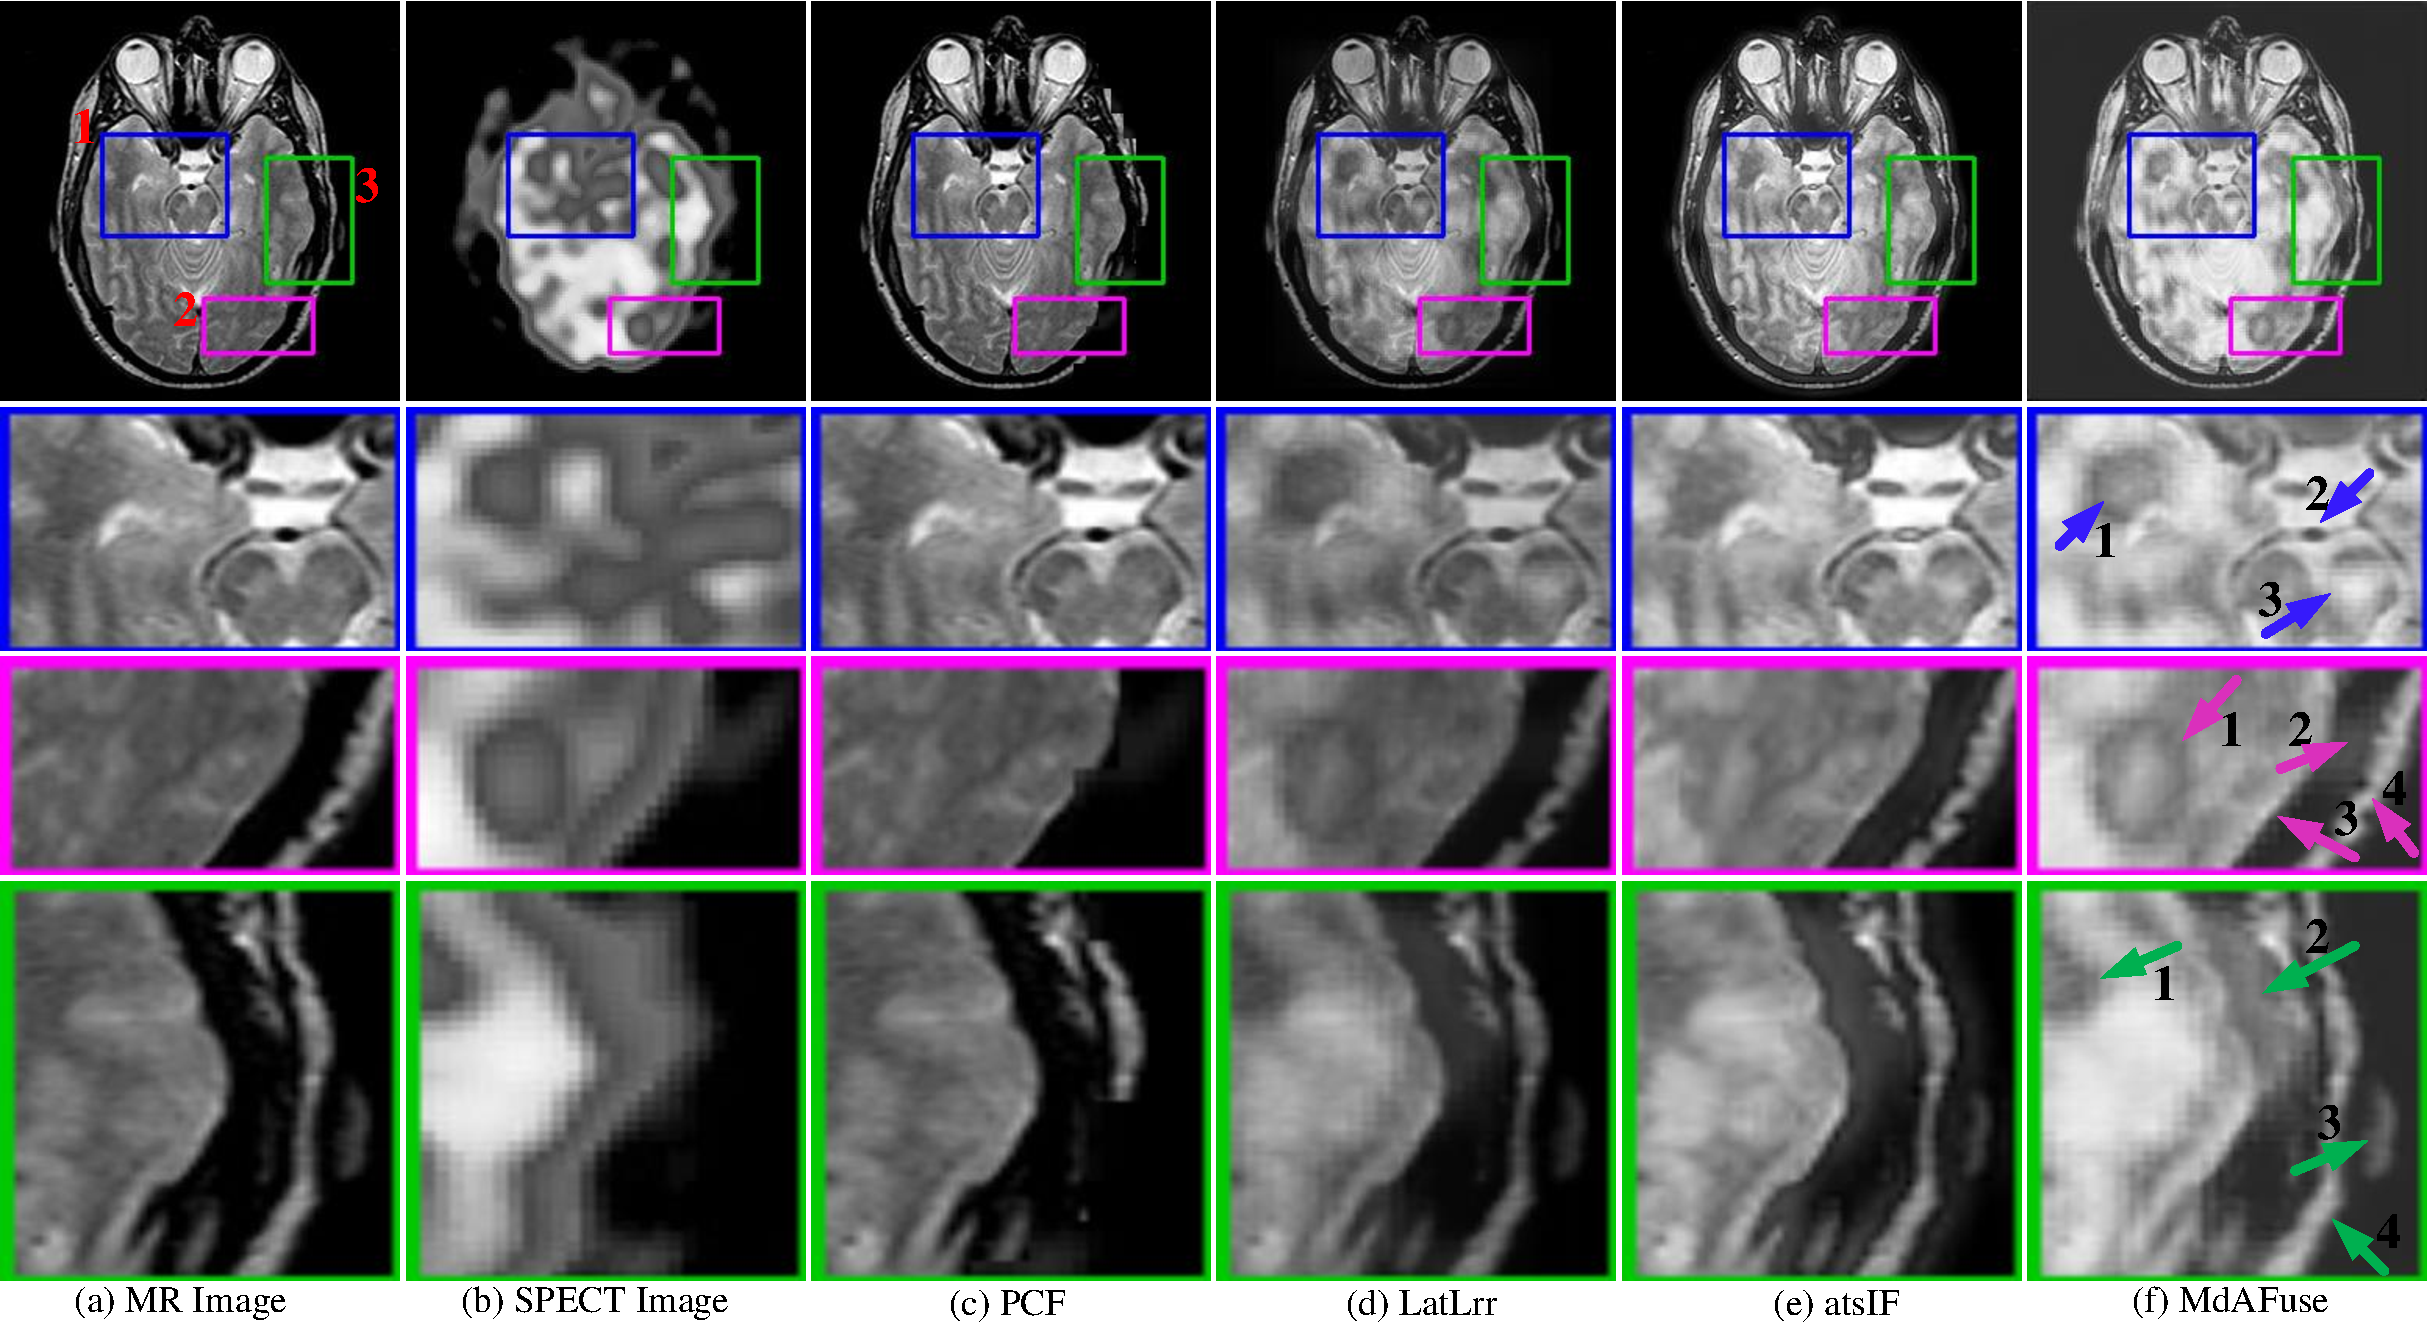
\includegraphics[width=0.9\linewidth]{figs/paper2d2_10_roi.pdf}
      \caption{比较传统的融合方法和本节提出的MdAFuse方法的MRI-SPECT融合结果}\label{paper2d2roi}
    \end{figure}
图\ref{paper2d2roi}中的第二行列出了与第一行中蓝色正方形内的部分相对应的放大影像。在最后一列,本节用三个箭头标记了颞叶、基底动脉和脑桥。颞叶在MRI上呈灰色,不规则。SPECT显示较浅的灰色圆圈,具有明显的色差。在PCF结果中,该区域不明显,MRI上的特征完全保留,但SPECT上没有。在LatLrr融合的结果中,该区域可以保留两个源影像的信息,但也丢失了部分SPECT信息,例如颞叶周围的像素值,这是没有区别的。atsIF方法的效果在亮度方面有了很大的提高,可以在SPECT中保留更多的信息,但合并后的源影像会出现信息丢失。与其他方法相比,本节提出的方法可以很好地保留颞叶区域的特征。对于基底动脉区,也注意到明显的差异。在MRI中,该区域是一个小的黑色椭圆,而在SPECT中,它是一个均匀的灰色区域,没有形状特征。PCF完全保留了MRI上的信息,LatLrr和所提出的方法显示该位置区域为深灰色,形状没有改变。atsIF的融合结果变成了一个白色区域,在小椭圆的外面有一个黑色的圆圈很明显。箭头3指向脑桥区,这是MRI上灰度分布不均匀的区域,SPECT影像上亮度明显且类似三角形的小区域。同样,在PCF的融合结果中找不到SPECT的特征信息,在LatLrr和atsIF结果中该位置区域的亮度信息也不明显。相对而言,本小节提出的方法的结果能清晰地反映MRI和SPECT的特征。

图\ref{paper2d2roi}中的第三行列出了与第一行中紫色方块内的区域相对应的放大影像。同样,在最后一列中,标记了指向枕叶、枕骨、侧窦和枕叶轮廓的四个箭头。从四个箭头的显示也证明了该方法的融合效果更好,尤其是在第一个箭头区域。图\ref{paper2d2roi}中的第四行列出了与第一行中蓝色方块内的部分对应的放大影像。最后一列中的四个箭头指向颞叶、颞肌、耳廓和外侧枕骨。从四个箭头的显示也证明了本小节方法的融合效果更好。

    \begin{figure}[ht]
      \centering
      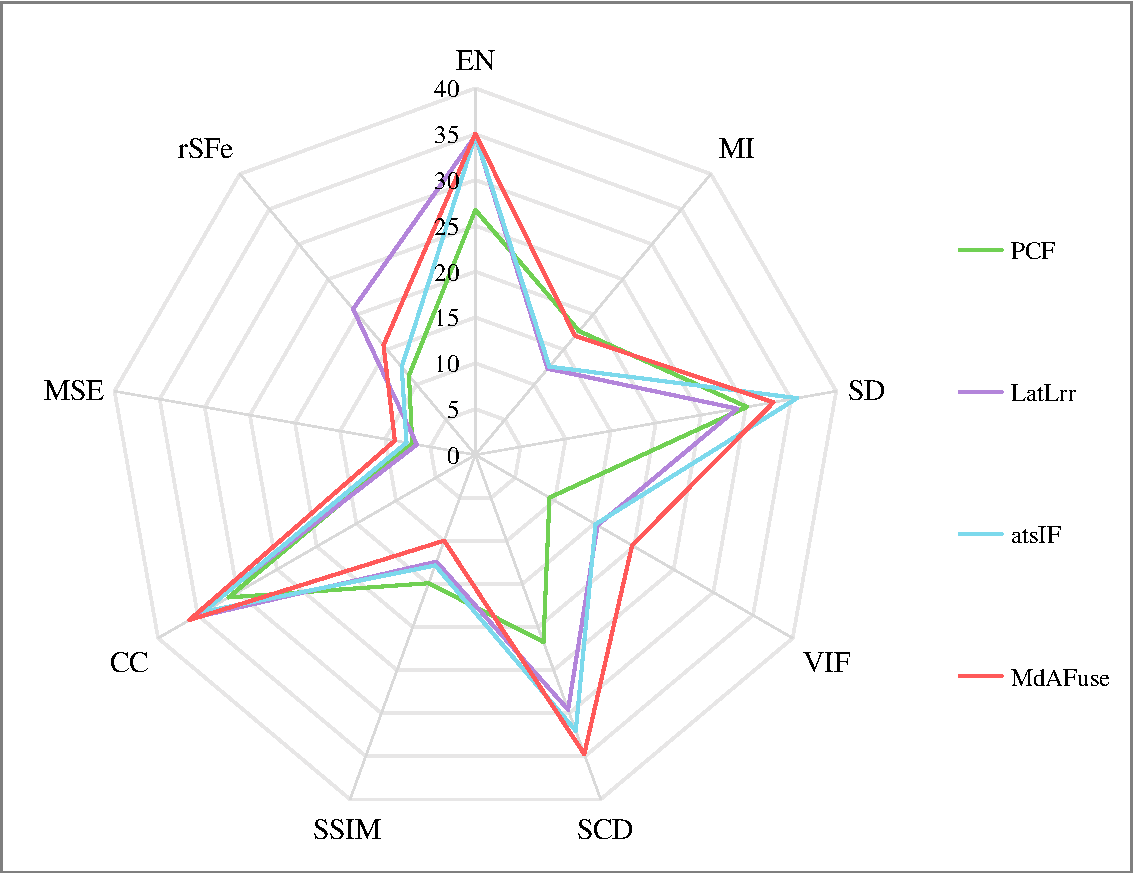
\includegraphics[width=0.9\linewidth]{figs/paper2traditionMetrics2024.pdf}
      \caption{图\ref{paper2d2roi}中与基于传统医学影像融合方法的客观评估比较分析}\label{paper2d2_10roi_value}
    \end{figure}

传统的影像融合方法主要属于像素级的融合操作,这种方法追求的是最大限度地保留信息。为了充分验证所设计的影像融合模型的实际效能,使用9个度量(EN,MI,SD,VIF,SSIM,SCD,CC,MSE,rSFe)来评估融合结果的质量,如图\ref{paper2d2_10roi_value}所示。在图\ref{paper2d2_10roi_value}中,可以观察到本节的MdAFuse方法的大多数度量都具有优势。具体地,SCD值比次优值高9\%。


\subsubsection{与新型方法的实验对比分析}
在这一部分中,对几种基于DL的影像融合方法进行了实验,并对它们的融合结果进行了比较。如图\ref{paper2029_1_roi}所示,第一列和第二列示出了要融合的MRI和SPECT源影像,并且随后的6列展示出了通过6种融合方法(包括所提出的方法:MdAFuse)获得的融合结果。从这些结果中,可以观察到不同的融合方法之间的差异。总体而言,可以观察到U2Fusion和CDDFused生成的融合影像似乎没有考虑SPECT的信息。虽然FusionDN和DeFusion方法保留了源影像中的SPECT信息,但仍然可以观察到一些信息丢失。FunFuseAn方法的影像融合效果相对较好,与本文提出的MdAFuse方法在视觉上具有相似性。因此,放大了三个小区域,以进一步比较和分析。在第一行中,使用三种颜色标记三个不同的区域并将其放大,如第二至第四行所示。



 \begin{figure}[ht]
      \centering
      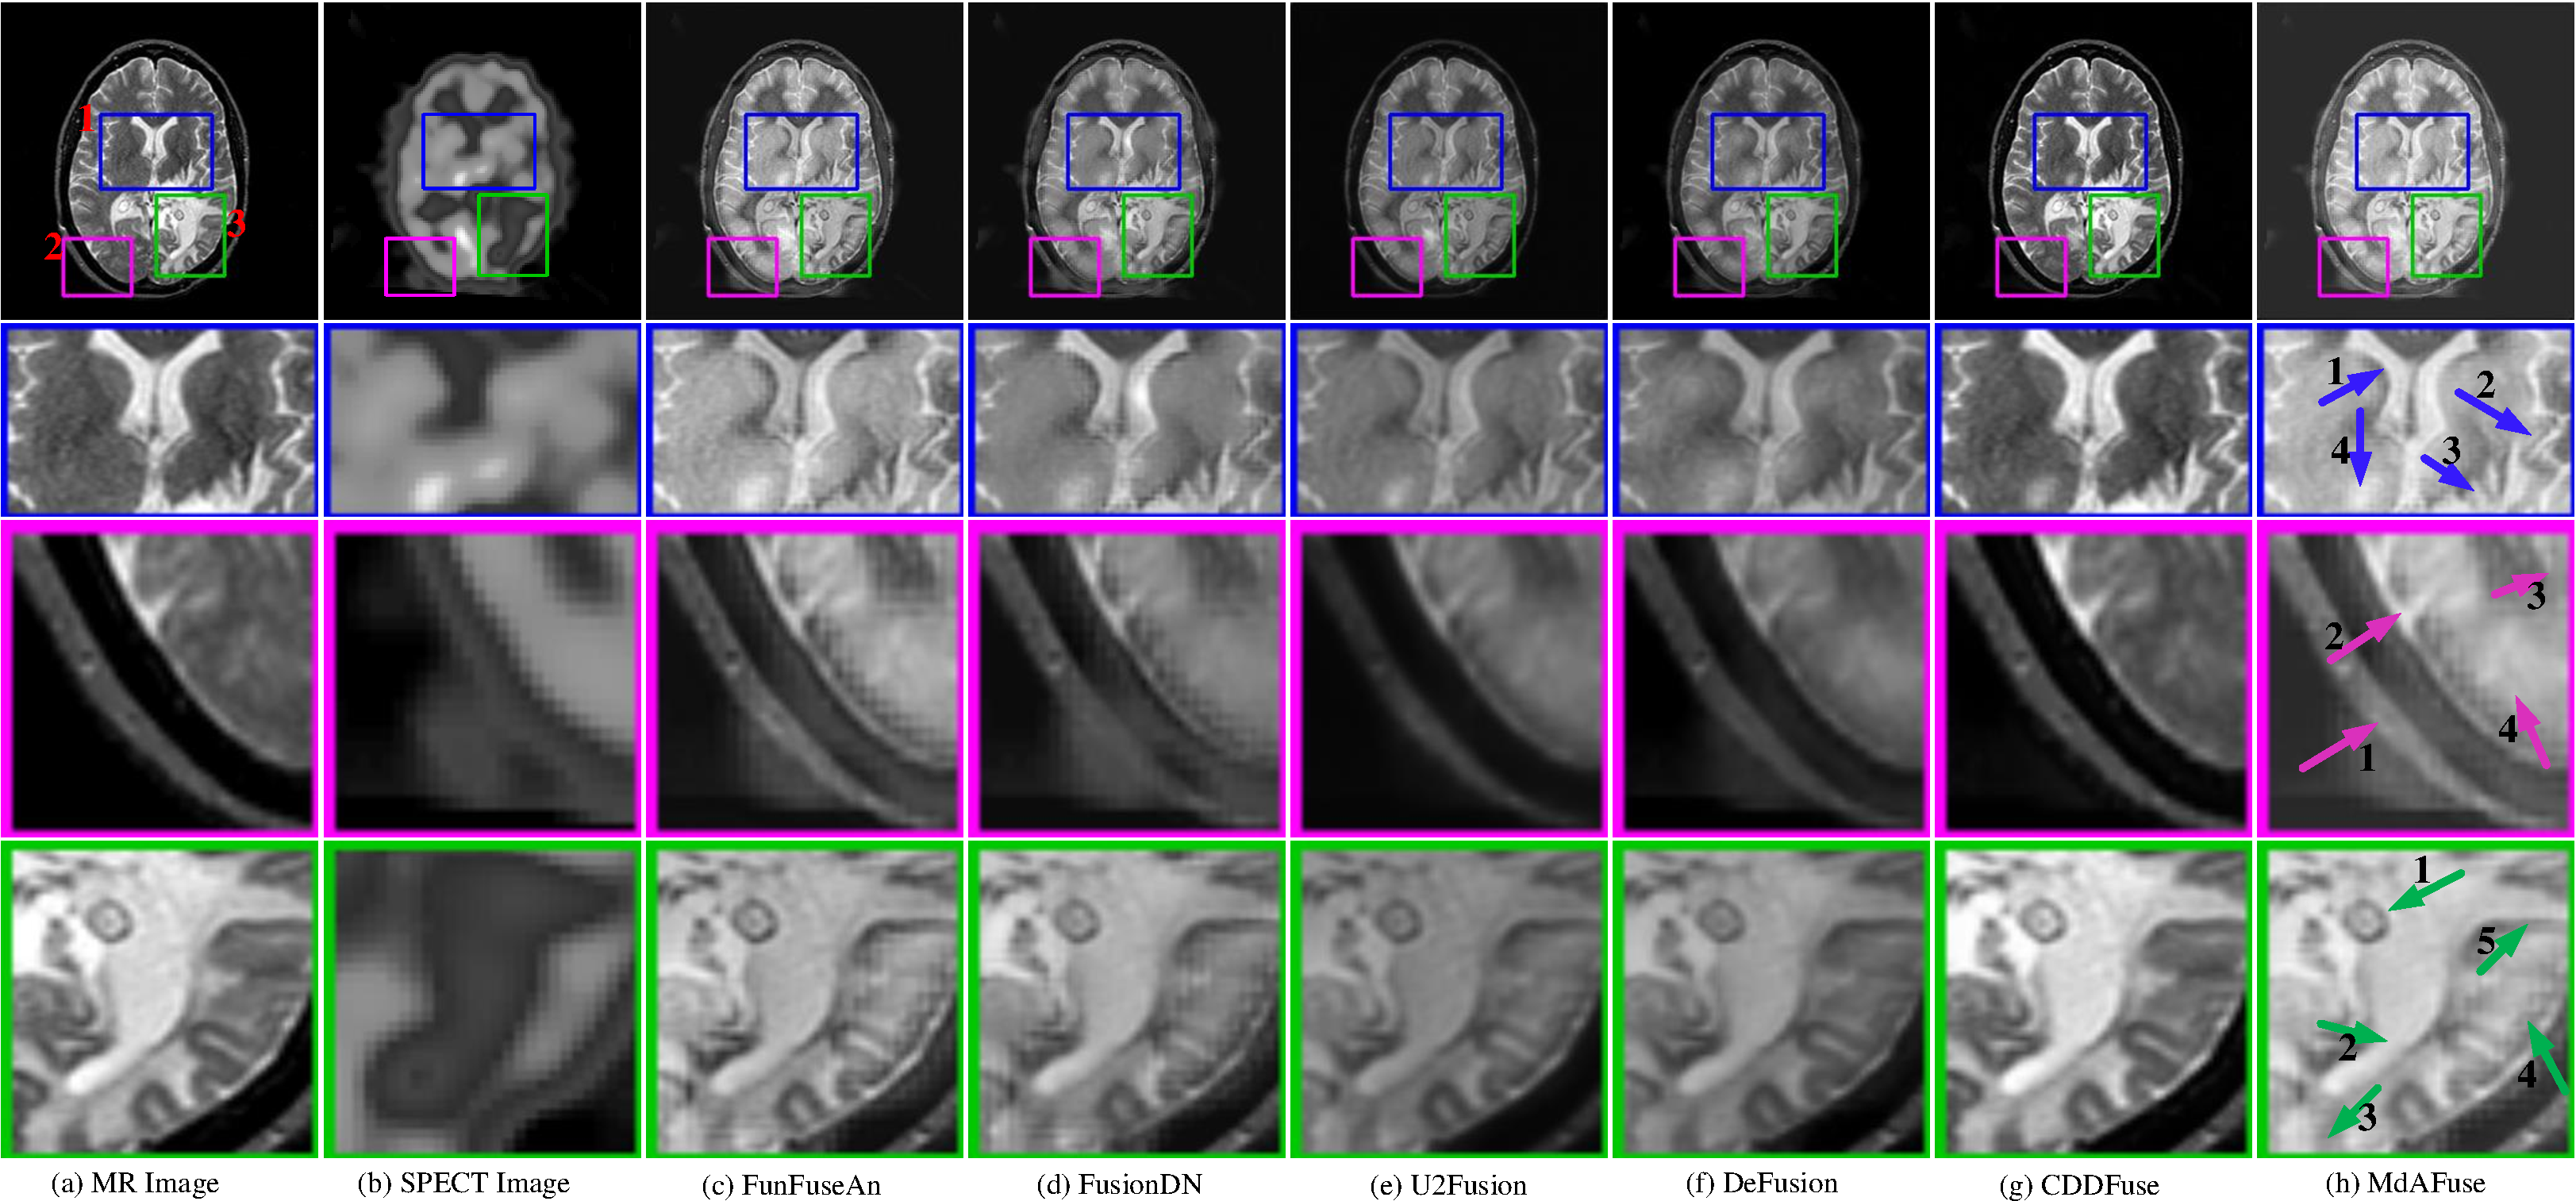
\includegraphics[width=0.9\linewidth]{figs/paper2_29_1_roi2024.pdf}
      \caption{本节提出的MdAFuse方法与现有的基于DL的方法性能比较}\label{paper2029_1_roi}
    \end{figure}

首先,图\ref{paper2029_1_roi}中蓝色方块标记的ROI主要反映侧脑室前角、丘脑和颞叶的信息。在MRI中,侧脑室的前角呈白色且对称,而在SPECT影像中,左侧脑室是灰色的。左侧丘脑区域在MRI中为深灰色,而晶状体区域在SPECT影像中为明亮。右侧丘脑区域呈白色,在MRI中看起来像丛林,而在SPECT影像中,它呈黑色,不规则。颞叶的面积在蓝色方块的左右两侧测量,主要反映在MRI上,是连续的。在图\ref{paper2029_1_roi}的最后一列中,四个区域用彩色方块标记。区域1为侧脑室左前角。
U2Fusion和DeFusion中这个位置的结构相对完整,但影像看起来模糊。CDDFuse突出显示MRI信息。FunFuseAn类似于FusionDN,两者都有色差。侧脑室左前角FusionDN较完整,而侧脑室右前角像素值分布不均匀。相比之下,MdAFuse可以更完整地保留MRI特征。区域2是颞叶。在FunFuseAn和FusionDN的结果中,结构相对完整和连续,但颜色相对较暗。U2Fusion和DeFusion的结果可以很好地保留MRI特征,但存在伪影。区域3是丘脑右侧的位置,在MRI上应该反映更多的纹理细节。在U2Fusion和DeFusion的结果中,位置不明显。FunFuseAn、FusionDN和CDDFuse很相似,组织结构不完整。相比之下,MdAFuse可以完全保留右侧丘脑。区域4为左侧丘脑,应显示一个亮点的扩散区。FusionDN和DeFusion的结果显示无明显状态。U2Fusion的结果可以识别出一个亮度块,但该区域的灰度值比较均匀,没有发现差异变化;其他方法可以明显地发现亮度块,可以检测出更多层次的亮度特征。

   \begin{figure}[htb]
      \centering
      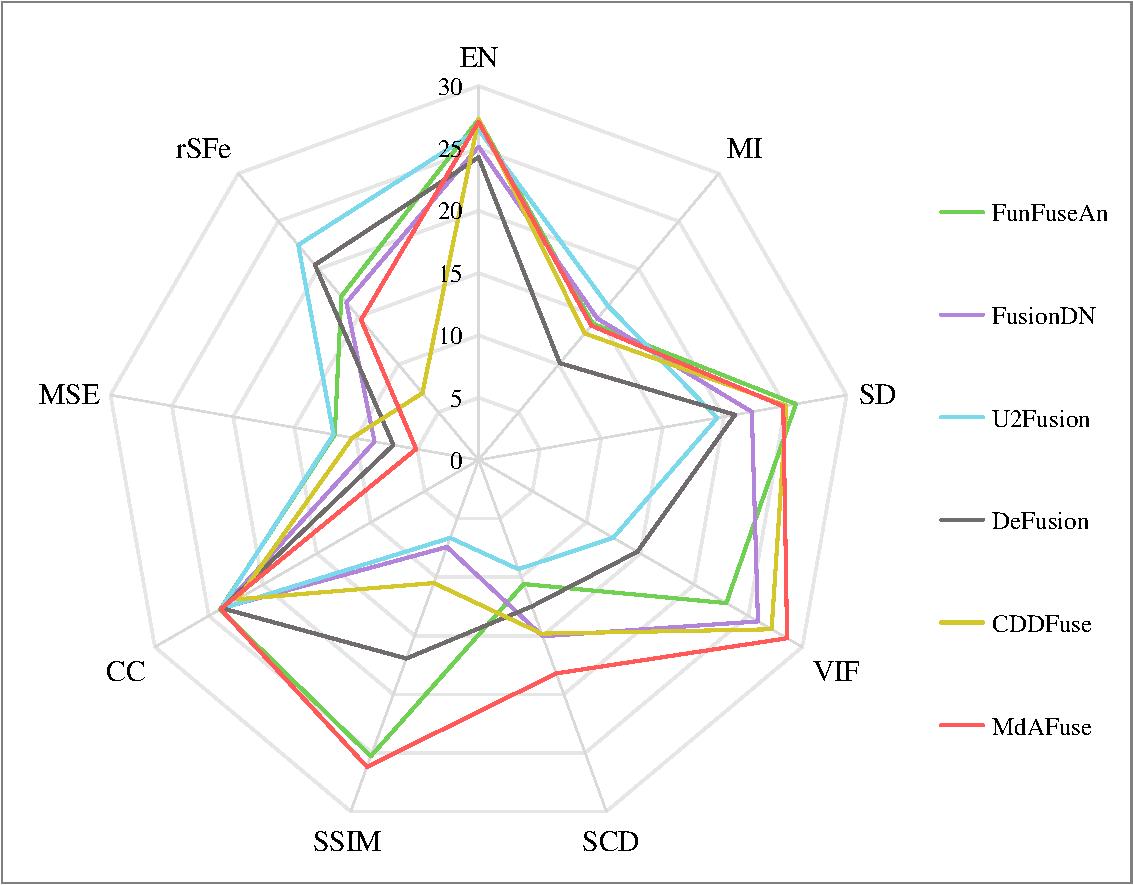
\includegraphics[width=0.9\linewidth]{figs/paper2DLMetrics2024.pdf}
      \caption{图\ref{paper2029_1_roi}中与基于DL医学影像融合方法的客观评估比较分析}\label{paper2029_1_roi_value}
    \end{figure}

其次,在图\ref{paper2029_1_roi}中放大的第二个紫色方块中,最后一列标记的四个区域是脑膜、枕叶、侧脑室枕角和大脑皮层(灰质)。在MRI中,ROI 1显示为粗灰色柱,而SPECT影像显示不均匀的波浪状灰色块。FusionDN和DeFusion的结果都显示出一些丢失,并且没有保留MRI的完整结构信息。U2Fusion和CDDFuse主要保留MRI信息,忽略SPECT特征。相比之下,FunFuseAn和MdAFuse考虑到了两幅原始影像中更重要的信息,并更完整地保留有用的特征。ROI 2是枕叶,在U2Fusion和DeFusion结果中不容易找到其。在FusionDN的结果中,未观察到位置区域与周围区域之间的显著差异。ROI 3是侧脑室的左枕角。可以在MRI上找到枕角的特征信息,这是SPECT影像上灰度值均匀的区域。FunFuseAn可以发现细微的变化,但本节的方法的结果更明显。箭头4指的是大脑皮层的一部分(灰质)。在这一区域的MRI中,可以发现一个灰度值分布不均匀的散在区域,并且可以观察到精细的纹理特征。在SPECT影像中,该区域是具有均匀灰度值的浅灰色。从测试结果来看,只有FunFuseAn和MdAFuse的灰度值层次结构比较突出,能够比较完整地保留MRI的特征信息,而其他方法的灰度值层次结果都难以识别。

最后,对于图\ref{paper2029_1_roi}中第三个蓝色正方形区域,信息量丰富,包括脉络丛、侧脑室枕角、枕叶、岛叶和小脑。五个箭头指向本节的方法的结果,这是明显不同于其他方法。区域1是脉络丛。在MRI中,整个位置是两个灰色同心圆。外圆的灰度值比内圆的灰度值深,差异明显。圆心的灰度值仅次于外圆,也比较突出。在SPECT影像中,灰度值更均匀。U2Fusion和DeFusion的结果显示,内圆的半径相对较大,圆心不明显,内圆区域的像素值没有差异。FunFuseAn,FusionDN,CDDFuse和本节的MdAFuse方法可以更好地保留MRI信息,并且可以清楚地找到内圈和外圈以及圆心之间的明显差异。类似地,其他箭头指向在本节的MdAFuse方法中获得更好的效果。

基于深度学习的融合方法主要可以从它们在特征级的操作来区分,同样地使用9个质量评估度量(EN、MI、SD、VIF、SSIM、SCD、CC、MSE、rSFe)来评估融合影像结果的质量,如图\ref{paper2029_1_roi_value}所示。从图\ref{paper2029_1_roi_value}中,可以观察到,与其他方法相比,本节的方法在6个指标上具有优势,特别是在SSIM,SCD,VIF和MSE中,与次优值的差异非常明显。对于rSFe度量,CDDFuse方法的值最小,但这个相对较小的值似乎有点异常。这可能是由于其较少保留SPECT影像中的信息,如图\ref{paper2029_1_roi}(g)所示。相比之下,本节的方法在这个指标上表现得更好。虽然在SD和MI指标上的表现并不突出,但与最大值和第二大值的差距并不明显。


    \begin{figure}[htbp]
      \centering
      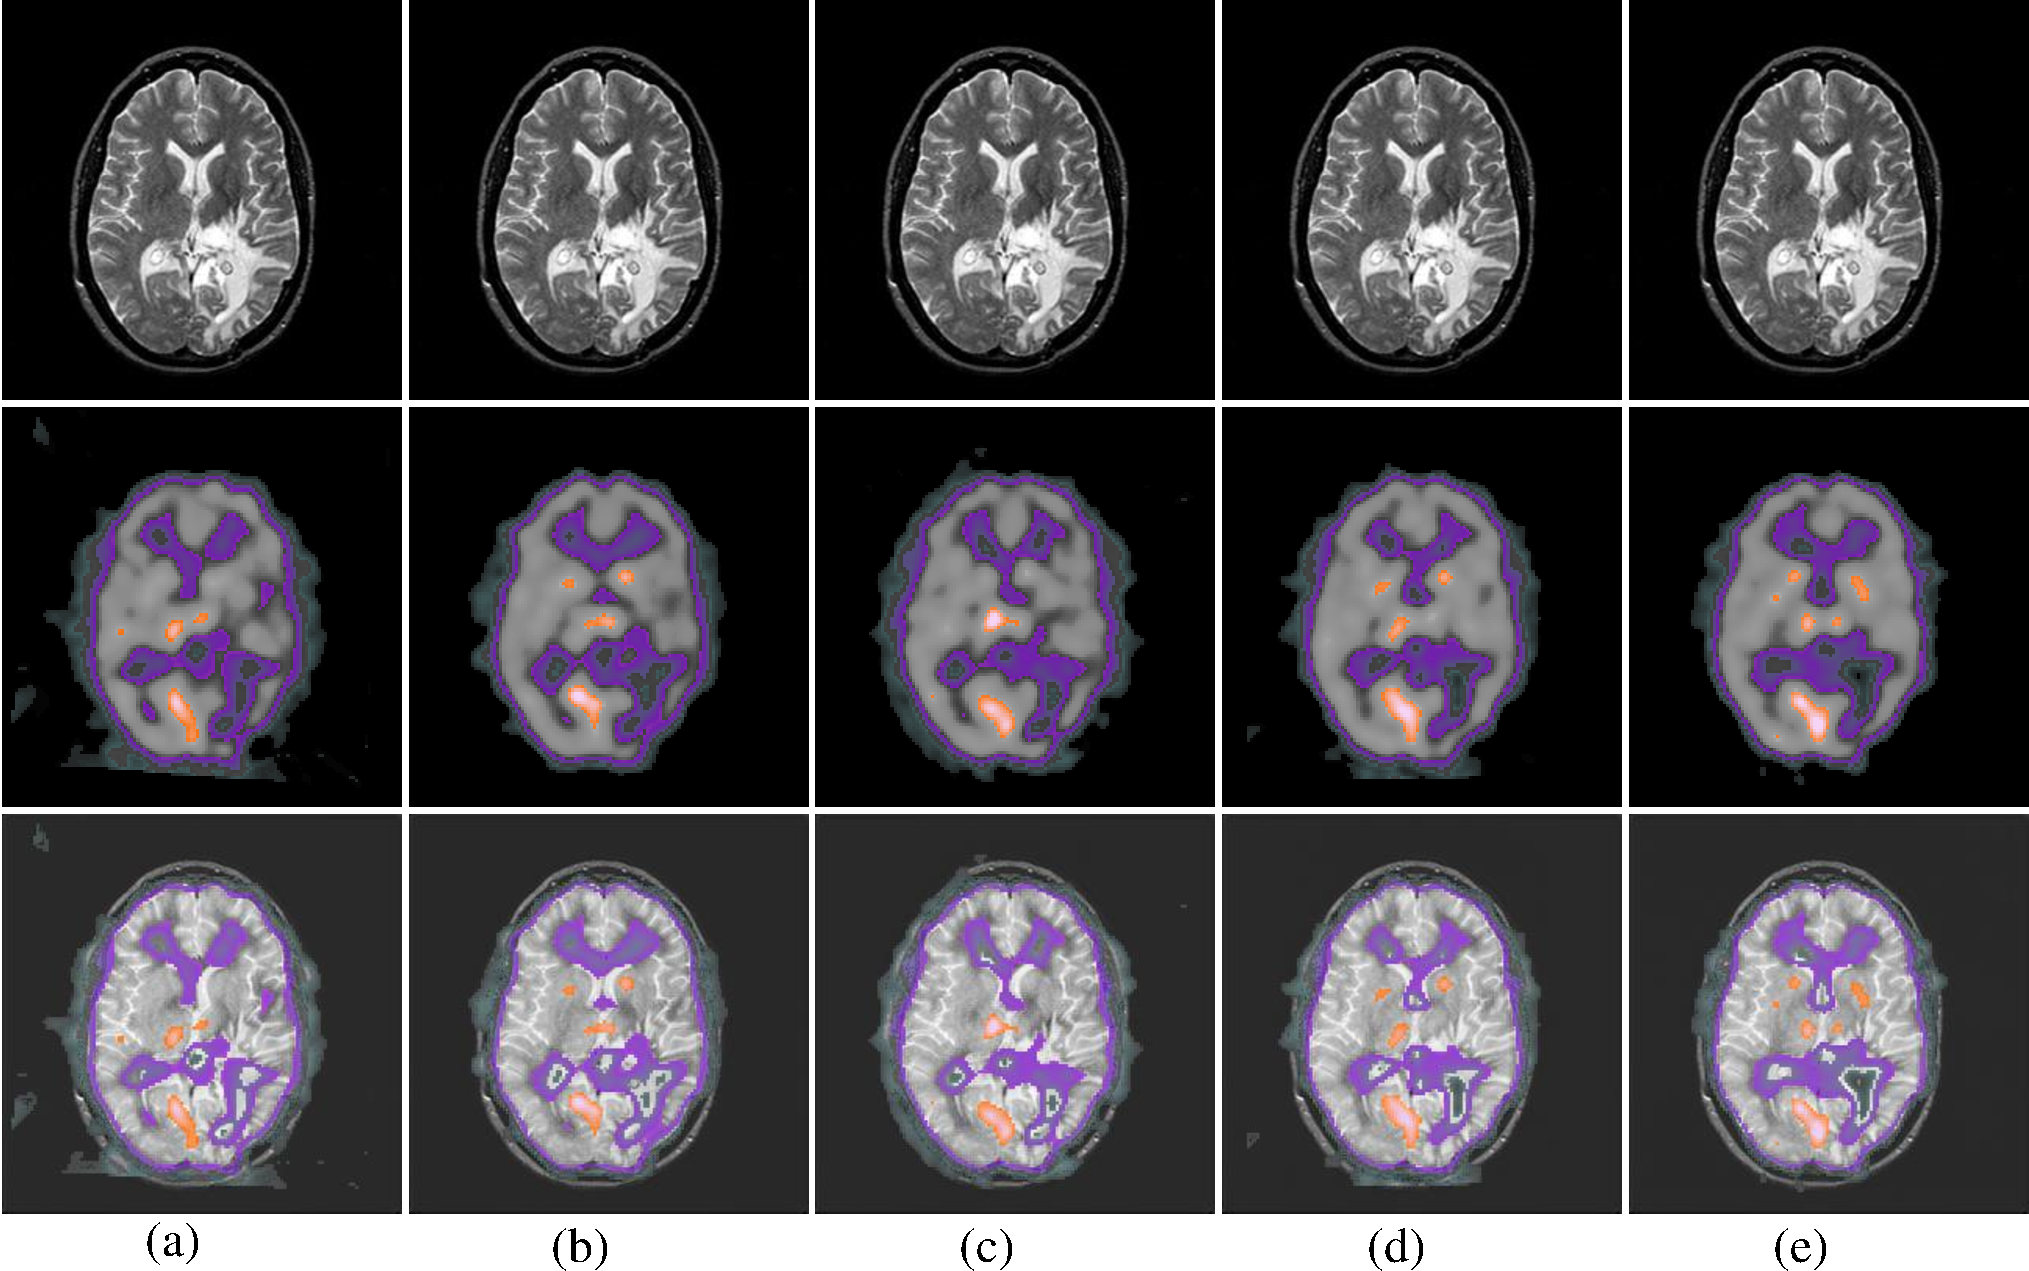
\includegraphics[width=0.9\linewidth]{figs/paper2029color.pdf}
      \caption{增强某一受试者融合影像中的关键特征}\label{paper2029_color_i}
    \end{figure}

采用74对MRI-SPECT、42对MRI-PET和21对MRI-CT医学影像融合结果与几种SOTA方法的定量分析结果见表\ref{paper2quantitativeMetrics}。表中的值表示每种方法在各种度量中的平均性能。在表\ref{paper2quantitativeMetrics}中,以粗体显示的值表示最佳值,而那些带下划线的值表示次优值。总体而言,本节的MdAFuse方法优于其他方法,在大多数指标中显示出上级结果,特别是在EN、VIF、SSIM和MSE上。CDDFuse是目前最先进的方法,当应用于MRI-SPECT融合时,本节提出的方法在VIF和SSIM中分别获得了11.14\%和18.38\%的提升。此外,本节提出的方法将MSE降低了2.63\%。在MRI-PET融合的情况下,本节的方法使得VIF和SSIM分别提高了13.76\%和5.61\%,而MSE降低了4.50\%。

\begin{table*}[htb]
\centering
  \caption{多模态医学影像融合结果与SOTA方法的定量比较与分析}\label{paper2quantitativeMetrics}
  \scriptsize
\begin{tabular}{cccccccccc}
\hline

\textit{MRI-SPECT} & \textbf{EN}     & \textbf{MI}     & \textbf{SD}      & \textbf{VIF}   & \textbf{SCD}    & \textbf{SSIM}   & \textbf{CC}     & \textbf{MSE}    & \textbf{rSFe}    \\ \hline
FunFuseAn                  & \underline{4.2348}    & \underline{2.6155}          & 55.3604          & 0.8947          & 1.0452          & \underline{ 1.5794}    & \textbf{0.8917} & 0.0535          & -0.3340          \\
FusionDN                  & 3.9001          & \textbf{2.6912} & 56.5726          & 0.5216          & 0.9051          & 0.4167          & 0.8756          & 0.0388          & -0.2623          \\
U2Fusion                        & 4.0581          & 2.4404          & 42.2308          & 0.3188          & 1.7674          & 0.3016          & 0.8832          & 0.0344          & -0.5399          \\
DeFusion                       & 3.7698          & 1.7543          & 49.9900          & 0.5393          & 0.7180          & 1.4480          & 0.8654          & \underline{ 0.0225}    & -0.3775          \\
CDDFuse                    & 3.9151          & 2.4925          & \textbf{58.3698} & \underline{ 0.9666}    & \underline{ 1.3458}    & 1.4717          & 0.8381          & 0.0375          & \textbf{-0.0449} \\
\textbf{MdAFuse}                    & \textbf{4.4135} & 2.5343    & \underline{ 58.0256}    & \textbf{1.0780} & \textbf{1.1483} & \textbf{1.6555} & \underline{ 0.8838}    & \textbf{0.0112} & \underline{ -0.2508}    \\ \hline

\textit{MRI-PET}            & \textbf{EN}     & \textbf{MI}     & \textbf{SD}      & \textbf{VIF}   & \textbf{SCD}    & \textbf{SSIM}   & \textbf{CC}     & \textbf{MSE}    & \textbf{rSFe}    \\ \hline
FunFuseAn                  & \underline{ 4.5540}    & \underline{ 2.5407}    & 57.5225          & \underline{ 0.7334}    & 1.1915          & 1.4668          & \textbf{0.8122} & 0.1123          & -0.3633          \\
FusionDN                  & 4.2210          & \textbf{2.6952} & \underline{ 64.5598}    & 0.4297          & 1.4188          & 0.4453          & 0.8024          & 0.0756          & -0.2153          \\
U2Fusion                        & 4.4952          & 2.0185          & 50.1283          & 0.3383          & \underline{ 1.5538}    & 0.2741          & 0.7760          & \underline{ 0.0453}    & -0.5511          \\
DeFusion                        & 4.1463          & 1.6765          & 63.5379          & 0.5199          & 1.4278          & 1.4335          & 0.7909          & 3.3017          & -0.2963          \\
CDDFuse                   & 4.2248          & 2.0258          & \textbf{70.7307} & 0.7056          & \textbf{1.6863} & \underline{ 1.4905}    & 0.7958          & 0.0700          & \textbf{-0.0316} \\
\textbf{MdAFuse}                    & \textbf{4.7241} & 2.3880          & 60.5385          & \textbf{0.8432} & 1.2910          & \textbf{1.5466} & \underline{ 0.8094}    & \textbf{0.0250} & \underline{ -0.3086}    \\ \hline

\textit{MRI-CT}             & \textbf{EN}     & \textbf{MI}     & \textbf{SD}      & \textbf{VIF}   & \textbf{SCD}    & \textbf{SSIM}   & \textbf{CC}     & \textbf{MSE}    & \textbf{rSFe}    \\ \hline
FunFuseAn                 & \underline{ 5.0245}    & \underline{ 3.1844}    & 58.5545          & \underline{ 0.6295}    & 0.9037          & \underline{ 1.5134}    & 0.8263          & 0.0940          & \underline{ -0.4218}    \\
FusionDN                   & 4.8268          & \textbf{3.2174} & \underline{ 69.0312}    & 0.3832          & 0.9328          & 0.4696          & 0.7698          & 0.1007          & -0.4246          \\
U2Fusion                     & 4.9148          & 2.1846          & 55.1028          & 0.3055          & \textbf{1.6707} & 0.4371          & \textbf{0.8347} & \underline{ 0.0460}    & -0.5763          \\
DeFusion                       & 4.6002          & 2.1969          & 66.1716          & 0.4649          & 1.1152          & 1.2976          & 0.8153          & 3.1185          & -0.4319          \\
CDDFuse                  & 4.8309          & 2.2431          & \textbf{79.4820} & 0.6100          & \underline{ 1.4100}    & 1.3094          & 0.8285          & 0.0753          & \textbf{-0.0255} \\
\textbf{MdAFuse}                    & \textbf{5.1195} & 3.0399          & 56.9286          & \textbf{0.6790} & 0.9250          & \textbf{1.5666} & \underline{ 0.8343}    & \textbf{0.0241} & -0.4661         \\\hline
\end{tabular}
\end{table*}

 
    \begin{figure}[htbp]
      \centering
      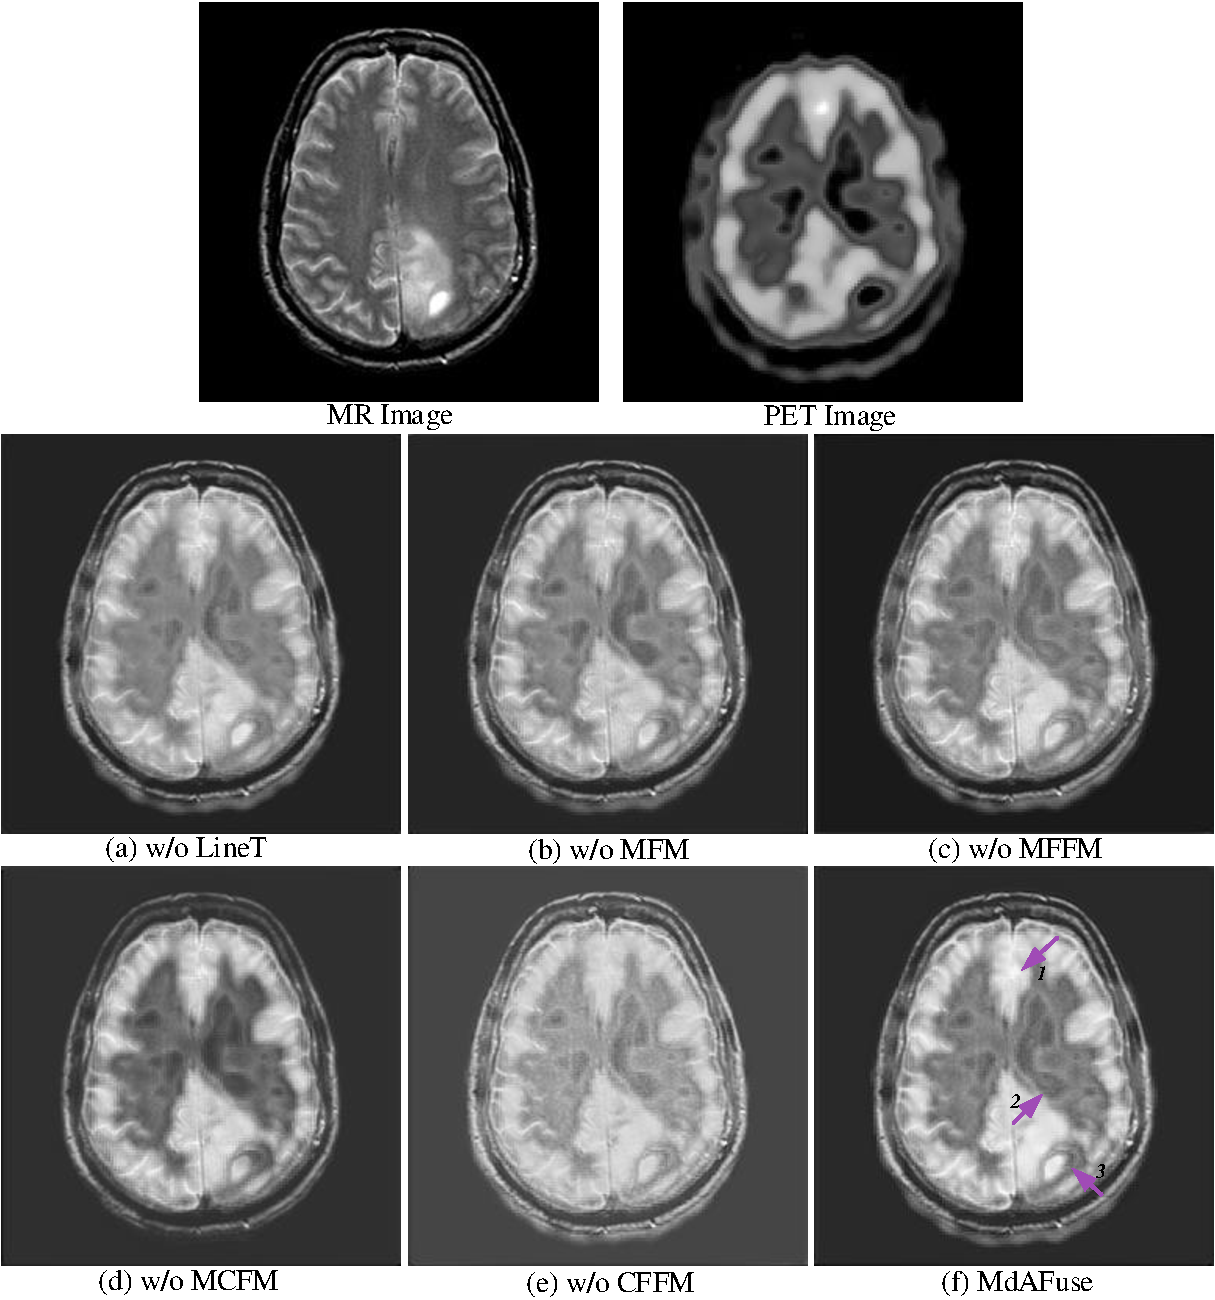
\includegraphics[width=0.85\columnwidth]{figs/paper2ablation1.pdf}
      \caption{本节所提出的影像融合方法的消融实验}\label{paper2ablation}
    \end{figure}

\subsubsection{脑影像的关键特征增强实验}
图\ref{paper2029_color_i}中的前两行显示了在五个周期内从具有脑异常的同一病例中采样的MRI-SPECT源影像。SPECT影像第二行的白色和黑色变化可用于确定病变的位置和病变的严重程度,有助于肿瘤的定位、分割和辅助诊断。第三行是前两行对应的MRI-SPECT影像对的融合结果,代表本节提出的方法的着色效果。从左到右的每列表示不同时间的成像结果。从图\ref{paper2029_color_i}中可以发现SPECT中能量信息的变化和容易判断异常的关键位置,主要体现在黄色轮廓和紫色区域。从左到右,融合结果上的黄色区域数量增加,左下顶叶的黄色区域增加,白色区域的亮度也提高。如果这种亮度代表较高的葡萄糖能量,则很可能在该位置发生糖尿病和高血糖。对于有黑点的区域,黑色块的数量随时间减少,但面积和浓度增加。例如,侧脑室枕角在图\ref{paper2029_color_i}(a)中只有一个小点,在图\ref{paper2029_color_i}(b)中形成两个小的蓝黑色区域。图\ref{paper2029_color_i}(c)中的黑蓝色区域的面积变大并向下移动,而图\ref{paper2029_color_i}(d)中的两个小区域合并,最后在图\ref{paper2029_color_i}(e)中面积扩大。表明该区存在异常。如果彩色区域代表细胞代谢能力,那么葡萄糖和蛋白质的严重缺乏可能会引起侧脑室枕角相应的疾病。因此,对融合结果进行着色可以增强融合后的效果,不仅可以揭示异常组织结构位置,还可以揭示能量变化,有助于准确诊断疾病演变。

\subsubsection{影像融合的消融实验}
为了充分说明浅层特征提取、深层特征提取、多尺度特征提取和线性变换融合策略的必要性和有效性,本节进行了五组消融实验,结果如图\ref{paper2ablation}所示。图\ref{paper2ablation}中的第一行表示一对多模态(MRI-PET)影像,第二至第三行展示出缺失线性变换操作的融合结果(w/o LinearT)、缺失多尺度特征提取模块(w/o MFM)、缺失多尺度和深层特征提取模块(w/o MFFM)、缺失多尺度和浅层特征提取模块(w/o MCFM)、缺失浅层和深层特征提取模块(w/o CFFM)以及所提方法的融合策略。在图\ref{paper2ablation}(f)中,三个箭头包含不同结果中的不同信息。在区域1中,应保留PET上的亮度信息。在图\ref{paper2ablation}(b)和图\ref{paper2ablation}(c)中,该位置的亮度不明显。在图\ref{paper2ablation}(a)和图\ref{paper2ablation}(d)中,位置模糊,这可能是由低亮度强度引起的。区域2是PET影像中的黑色区域,并且在MRI中灰度不均匀。在图\ref{paper2ablation}(b)和图\ref{paper2ablation}(d)中,它是具有均匀灰度级的区域。在图\ref{paper2ablation}(a)和图\ref{paper2ablation}(c)中,灰度级以特定梯度布置,但是边缘出现平滑现象。在图\ref{paper2ablation}(f)中,效果更好,并且保留了更多的结构信息。MRI上箭头3所指的区域是一个比扁豆大的小区域,亮度强而均匀,与周围的色差有层次关系。在这六种情况下,本节的MdAFuse方法都能反映出该位置的增强效果,取得了较好的效果。

  \begin{figure}[htbp]
      \centering
      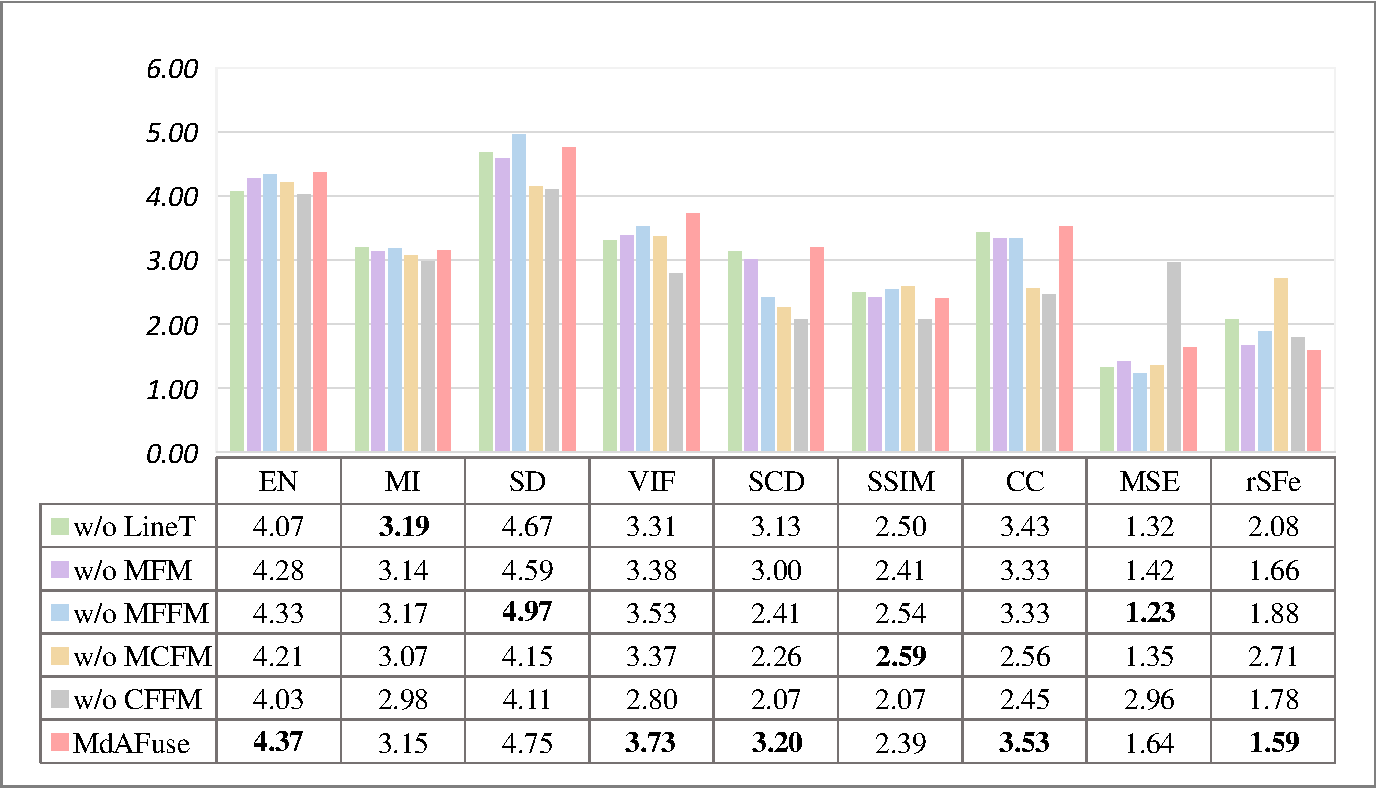
\includegraphics[width=0.9\columnwidth]{figs/paper2ablation2024_value1.pdf}
      \caption{消融实验结果(图\ref{paper2ablation})的9种质量评价指标显示}\label{paper2ablation_value1}
    \end{figure}
    
图\ref{paper2ablation_value1}显示了一些用于质量评估的指标值。在图\ref{paper2ablation_value1}中,下半部分是原始的六个度量值,上半部分是条形图显示。为了更好地观察和比较同一图表中不同的度量值,对每个度量值进行了线性变换,变换系数如表\ref{lineTransformation}所示。在图\ref{paper2ablation_value1}中,可以观察到本节的方法在5个指标中具有最优值,在1个指标中具有次优值。因此,相比较而言,本节提出的方法表现出了最佳的性能。因此,也说明了本节提出的MdAFuse方法对于其他融合方法在9种客观评估指标上的结果是最好的,这也证明了通过增加多维特征并使用自适应融合策略构建的网络可以获得更好的融合结果。
    

\subsection{小结}
在这小节中,本节提出了一种新的基于DL的融合框架,结合空间特征和通道特征的多维特征。同时,采用深度分离卷积网络,挖掘更丰富的有用信息,可为源影像提供显著特征和丰富细节特征,供后续影像理解和应用分析。采用三种不同的特征提取模块和一种基于各维特征相关性的自适应线性融合机制来保留MRI的空间纹理信息和PET/SPECT影像的生理代谢信息。此外,本节还提出了一种关键特征增强方法,该方法可以增强同一病例不同时期融合影像的可视化效果,有助于肿瘤定位、分割和疾病跟踪等临床应用。不同的疾病采用不同的常用影像学检查进行评价,多模态医学影像融合也是多种多样的。后续工作将持续研究不同类型的医学融合方法,并将其应用于人工智能医学诊断。

虽然本节的方法在MRI-PET/SPECT影像融合中表现出了一定的优势,但仍然存在一些局限性。本节的方法只关注MRI和PET/SPECT影像的关键特征,而不考虑某种疾病的特异性。此外,对于大脑影像的融合,没有增加对潜在疾病区域的神经科学分析。将联合神经科学与人工智能方法更深入地结合将是今后研究的一个有意义的方向。


\section{本章小结}
在\ref{chapter3.1:MsgFusion}节中,本节介绍了一种基于MS-Info引导的脑部疾病影像深度特征融合方法,被称为MsgFusion。该方法通过分析MRI/CT/PET/SPECT的关键MS-Info,获取相应的影像特征,并设计了一个包括SF-Branch和GV-Branch的双分支网络。SF-Branch结合了空间域和频域信息,GV-Branch结合了HSV颜色空间的多尺度灰度影像和亮度。这一双网络机制成功提高了CNN的泛化能力,充分考虑了频域信息和颜色空间信息的重要性,确保了融合结果的有效性。实验证明,在医学脑影像的处理和分析中,包括MRI-CT影像融合、MRI-SPECT影像融合和MRI-PET影像融合等方面,该方法相较于现有方法具有显著优势。通过临床医生的问卷调查评估和统计数据的支持,MsgFusion的融合效果被证实为最佳。

在\ref{chapter3.2:MdAFuse}小节中,本节提出了一种新的基于DL的融合框架,被称为MdAFuse,采用了空间特征和通道特征的多维度结合。引入深度分离卷积网络,旨在挖掘更丰富的有用信息,为源影像提供显著特征和丰富细节特征,以支持后续影像理解和应用分析。提出了三种不同的特征提取模块和一种基于各维特征相关性的自适应线性融合机制,以同时保留MRI的空间纹理信息和PET影像的生理代谢信息。此外,本节提出了一种关键特征增强方法,可提升同一病例不同时期融合影像的可视化效果,有助于肿瘤定位、分割和疾病跟踪等临床应用。考虑到不同疾病使用不同常用影像学检查进行评价,未来将持续研究和拓展多模态医学影像融合方法,以适应人工智能医学诊断的不断发展。
尽管本节的方法在MRI-PET/SPECT影像融合中表现出一定的优势,但仍存在一些局限性。本节的方法侧重于提取MRI和PET/SPECT影像的关键特征,而未考虑某种疾病的特异性。此外,在大脑影像的融合中,本节未加入对潜在疾病区域的神经科学分析。

未来,计划扩展框架,将两种以上的医学影像进行融合,并应用于更广泛的临床诊断场景。另外,将更深入地探讨如何将神经科学与人工智能方法更加紧密地结合,以实现更全面和准确的医学影像融合。

%%% Local Variables:
%%% mode: latex
%%% TeX-master: "../main"
%%% End:

% !TEX root = ../main.tex
\chapter{阿尔茨海默症的智能辅助分类} 
\label{chapter:fineClassify}
当前神经网络驱动的图像分类算法普遍存在仅能捕获局部空间特征的问题,这在一定程度上制约了特征抽取的有效性,进而可能影响到分类性能的整体准确性。特别是在AD早期阶段的诊断分类任务中,面对从EMCI、MCI到LMCI这一连续进展阶段的精细化分类任务,亟需发展更加稳健且智能的分类策略,以实现对疾病进程的精准评估与预测。
在这一章中,将介绍一种以影像为导向的新小波卷积单元神经网络。一方面,为了获得非局部的感受野以及避免信息丢失,本章定义了一个新的卷积运算单元。使用该小波卷积单元,进一步设计了一个基于它的细粒度AD多分类网络\cite{wen2023fine},在细粒度多分类任务上实现了更高的分类精度。
%到目前为止,只有少数方法研究了一种或多种AD的细粒度分类,能够同时实现细粒度和多类分类的方法更少。本章采用了新的网络在DTI影像上实现细粒度分类,达到了较先进的水平。
%,实验得到的八种细粒度分类的准确率分别为97.30\%,95.78\%,95.00\%,94.00\%,97.89\%,95.71\%,95.07\%,93.79\%。
%为了建立AD分类的参考标准,本章实现了所有粗粒度和细粒度的12种分类。结果表明,本章提出的方法实现了更高的分类精度。

\section{引言}
AD是在老年人群中非常常见的一种疾病。目前,还没有有效的治疗方法可以治愈AD或改变其进展。MCI是介于AD和NC之间的中间阶段。临床研究表明,MCI可分为EMCI和LMCI。EMCI阶段是可逆的,及时发现和干预可以避免AD的发展,而在LMCI阶段及时诊断和治疗可以延缓AD的发展或治愈AD,因此痴呆的早期发现和诊断将成为主要目标。AD的早期准确诊断是一个有意义和挑战性的任务。


卷积神经网络在非医疗影像分类领域取得了显著成效,因此众多研究开始探索将其技术应用于医学影像分类以及智能化辅助疾病的诊断。尤其是在过去的十年间,学者们提出了一系列基于深度学习技术针对AD分类的方法,如表\ref{paper3accuracy1}所示。但同时,这些现有方法也暴露出一些局限性问题。
\begin{itemize}
    \item 当前大多数运用深度学习技术对AD进行分类的方法,通常采用的是为非医学影像设计的标准卷积操作,其局限性在于局部感受野受限。尽管空洞卷积能有效拓宽局部感知范围,但同时也会导致大量信息的丢失问题。与自然图像不同,整个医学影像中的细节特征都比较重要。另外,细粒度AD分类的实现和准确性面临着一定的挑战和瓶颈。为了更有效地提取医学影像的深度特征,需要一种新的非局部感受野卷积运算。
    \item 现有的大多数AD分类方法只能实现粗粒度的分类。只有少数方法,例如\cite{Fangmeie2022,de2021dti},研究了某些类型的细粒度分类,而细粒度的分类具有更重要的临床意义。此外,AD分类方法很多,但它们所能实现的分类组合参差不齐。需要一种能够实现12种全分类的方法,为该领域的研究提供参考。
    \item 大多数现有的工作采用MRI数据进行AD分类。根据临床医学理论,DTI反映了脑内纤维束间组织结构的连续性,与AD密切相关。因此,本章选择DTI进行细粒度的AD分类。
\end{itemize}

关于DTI数据的选择,本章给予以下详细的解释。神经影像学检查的方式(包括DTI扫描、正电子发射断层扫描(PET)扫描、MRI扫描等)通常用于AD的诊断。DTI\cite{huynh2019multi}也称为基于水分子运动的特殊MRI模态。DTI成像的原理是水分子在梯度场中的扩散改变磁矩。因此,这项创新技术能够清晰展示大脑白质区域中神经束的布局,以揭示人体中枢神经系统的纤维构造细节。脑中纤维束之间组织结构的连续性可以从水中扩散纤维束的成像中推断\cite{frisoni2010clinical}。在AD患者的研究中,DTI影像显示为灰质、白质等的FA(各向异性分数)异常降低和MD(平均扩散率)值异常增加。因此,与其他影像数据相比,DTI数据更有利于实现早期的细粒度分类。

为了突破现有AD分类方法的上述局限性,本章将小波理论应用于卷积运算中,定义了一种新的卷积单元,并将单尺度和多尺度小波分解的特征融合在一起,以获得非局部的感受野,避免信息丢失。采用新的小波卷积单元(wavelet convolution unit,WCU),本章基于DTI数据实现了12种所有组合分类,特别是对于细粒度分类,提高了分类精度。
总之,本章提出了一个小波卷积单元来构建一个有效的WCU网络,用于细粒度和多AD分类。使用WCU的深度学习方法和DTI数据主要证明本章提出的方法实现了更高精度的细粒度AD分类。
本节工作的三个主要创新点:
\begin{itemize}
    \item 本章提出了一种新的卷积单元(WCU),将小波变换与传统的卷积函数相结合,以获得非局部的感受野,避免信息丢失。嵌入WCU的网络大大提高了卷积神经网络的性能。WCU是首个将小波分析嵌入到初级的卷积神经网络中的智能辅助阿尔茨海默症分类的工作。
    \item 本章提出了一种基于WCU和脑影像DTI数据的AD分类网络框架(WCU-Net)。首次实现了所有粗粒度和细粒度的组合分类。大多数现有的AD分类方法限于AD与MCI与NC之间的粗粒度分类,少数方法实现了一种或几种细粒度分类。本章所提出的方法实现了所有八种细粒度分类,其中,首次出现细粒度三分类。该方法为以后的AD分类研究提供了参考标准。
    \item 本章的工作实现的所有12种分类获得了高准确率,特别是对8种细粒度分类的准确率从92.5\%,92.6\%,93.5\%,90.9\%,81\%,无,无,92.6\%提高到97.30\%,95.78\%,95.00\%,94.00\%,97.89\%,95.71\%,95.07\%,93.79\%。首先,提出了细粒度的三分类方法,准确率达到95\%以上。细粒度二分类EMCI与LMCI相比,分类准确率提高了16.89\%。细粒度四分类的准确率达到93.79\%,比现有方法提高了1.19\%。此外,通过使用来自合适的预训练经典网络模型的初始权重,可以进一步提高准确性。
\end{itemize}


\ref{chapter4.2}节简要介绍了包括小波分析在内的频域分析方法及其在图像处理中的应用,并介绍了基于神经网络的AD辅助诊断和分类的研究现状。\ref{chapter4:WCU-net}节详细介绍了新的小波卷积单元、基于WCU的神经网络框架和训练方法。\ref{chapter4.4}节描述了基于WCU-Net的AD细粒度多分类方法在脑DTI影像数据上的实现,并进行了一系列的实验和结果分析。最后,\ref{chapter4.5}节对本小节的工作进行了总结,并提出了未来的研究方向.


\section{相关工作}\label{chapter4.2}

\subsection{基于传统智能辅助分类技术}
在AD的分类任务中,传统的方法大多集中于AD、NC和MCI的粗分类\cite{payan2015predicting}。Xiao等人\cite{xiao2017brain}提出了一种新的分类框架,以准确识别AD患者。该方法分析了多特征组合相关技术,并利用协方差法对SVM-RFE算法进行了改进,结果表明多特征组合方法优于单特征方法。白质(White matter,WM)损伤是AD病理级联反应的重要组成部分,在AD的诊断中常被忽视\cite{rathore2017review}。研究白质最有力的工具是DTI,它是一种无创的体内成像技术。通过色散特性识别白色物质纤维趋势和损伤程度可以揭示AD的结构完整性并描述白质的恶化\cite{horgusluoglu2020systems}。Ben Ahmed等人\cite{ahmed2017recognition}提出从DTI和sMRI中提取局部影像衍生的生物标志物,以构建多模态AD特征。很少有学者采用常规方法进行细粒度的二分类\cite{prasad2015brain}。Ashburner和Friston\cite{ashburner2000voxel}提出了一种基于体素形态测量的传统特征表示的方法。Zhang等人\cite{zhang2016detecting}提出了一种基于地标的形态特征方法。

\subsection{基于新型智能辅助分类技术}
患者往往在被确诊患有AD时已经发展到疾病的中期或晚期。鉴于此,在利用人工智能进行AD的早期诊断时,迫切需要一个既具备高灵敏度又具有高效率的诊断方案\cite{shehata2018computer,bringas2020alzheimer,liu2018joint}。近年来,随着DL在各个领域取得的优异成绩,DL逐渐在医学领域得到广泛应用。CNN是最常见的深度学习方法,由于其在影像分析和分类领域的成功而受到广泛关注\cite{golla2020convolutional,liang2021cameranet}。尽管如此,深度学习技术在诊断AD时面临巨大挑战,这主要归因于医学影像数据缺乏适当的预处理、存在采集误差以及知识库的不足。Aderghal及其同事\cite{aderghal2017classification}设计了一种专门针对结构性磁共振成像(sMRI)扫描特性的数据增强方法,以优化连续切片样本的训练与分类过程。另一方面,Lei\cite{lei2016discriminative}探索了一种融合MRI与PET数据的判别式特征学习技术。多模态成像融合手段在增强对AD的诊断准确度方面具有明显优势,但其涉及的多步骤影像处理流程常常导致预处理阶段所需时间增加。
为克服这一问题,Fang等人的研究\cite{fang2020ensemble}中创新性地构建了一个新框架,该框架整合了三种最先进的深度卷积神经网络模型,并应用于多模态影像数据,旨在提高AD分类任务的精确度。

在AD分类任务中,主要使用MRI数据,如AD和NC的二分类\cite{xing2020dynamic,ebrahimi2021convolutional},以及AD,MCI和NC的三种成对组合\cite{ahmed2015alzheimer,yang2017active,madusanka2019alzheimer,pan2020early,liu2022diagnosis}。文献\cite{vu2018non}描述了一种用于检测和识别AD的MRI和PET影像的自动化和稳健的方法。Bi等人\cite{bi2020computer}提出了一种新的深度学习技术应用于AD的预测。该方法在AD与NC分类中的准确度比较,MCI分型为91.25\%。DTI已间歇性用于识别AD的分类任务\cite{qu2021ai4ad,lella2021ensemble},实现了二分类(AD与NC),准确度分别为0.885,0.8235。Ebadi等人\cite{ebadi2017ensemble}研究了关于通过使用集成分类模块执行分类任务来应用大脑连接模式辅助诊断AD和MCI的潜力。表\ref{paper3accuracy1}列出了这些方法和相应的分类精度,表中的每种粗粒度分类的最高准确率和次高准确率分别用红色和蓝色标记 (D-1: AD vs. NC, D-2: AD vs. MCI, D-3: MCI vs. NC, T-1: AD vs. NC vs. MCI)。

\begin{table*}[ht]
\centering
\caption{AD的粗粒度分类的相关工作及其相应的准确率}\label{paper3accuracy1}
\footnotesize
\begin{tabular}{p{3.7cm}<{\centering}|p{1.8cm}<{\centering}|p{1.35cm}<{\centering}|p{1.35cm}<{\centering}|p{1.35cm}<{\centering}|p{1.35cm}<{\centering}}
\hline
\multicolumn{1}{c|}{\multirow{2}{*}{ Methods }}
& \multicolumn{1}{c|}{\multirow{2}{*}{Modality}}
& \multicolumn{4}{c}{Accuracy ("-": not classified)}
\\ \cline{3-6}
\multicolumn{1}{c|}{}                         & \multicolumn{1}{c|}{}                       & \multicolumn{1}{c|}{ D-1 } & \multicolumn{1}{c|}{ D-2 } & \multicolumn{1}{c|}{ D-3 } & \multicolumn{1}{c}{T-1} \\ \hline
Ben Ahmed et al. \cite{ahmed2015alzheimer} & MRI  & 0.838 & 0.695 & 0.621 & - \\

Payan and Montana \cite{payan2015predicting} & MRI  & 0.954 & 0.868 & 0.921 & 0.895 \\

Aderghal et al. \cite{aderghal2017classification}          & MRI & 0.914 & 0.695 & 0.656  & -  \\
Yang et al. \cite{yang2017active}  & MRI  & 0.91  & 0.877 & 0.855  & -  \\
Xiao et al. \cite{xiao2017brain}    & MRI & 0.8571 & 0.7944 &0.8611 & 0.75 \\
Madusanka et al. \cite{madusanka2019alzheimer}              & MRI & 0.8661  & 0.8205 & 0.7896 & - \\
Bi et al. \cite{bi2020computer}    & MRI  & 0.8915  & \textcolor{red}{{0.9701}} & 0.926  & \textcolor{blue}{{0.9125}} \\
Duc et al. \cite{duc20203d}         & MRI & - & -  & - & 0.8715\\

Xing et al. \cite{xing2020dynamic} & MRI  & 0.92 & -  & - & -    \\
Pan et al. \cite{pan2020early}     & MRI  & 0.89 & 0.83  & 0.68  & -\\
Ebrahimi and Luo \cite{ebrahimi2021convolutional}            & MRI  & 0.9375  & -  & -  & -   \\
Liu et al. \cite{liu2022diagnosis} & MRI & \textcolor{blue}{{0.9896}}  &0.9537 &0.926 & - \\
\hline
Lei et al. \cite{lei2016discriminative}               & MRI+PET   & 0.969& -  & 0.866 & -   \\
Vu et al. \cite{vu2018non}         &  MRI+PET   & 0.988 & 0.93  & \textcolor{blue}{{0.95 }} & 0.9113 \\
Ben Ahmed et al. \cite{ahmed2017recognition}                & MRI+DTI   & 0.902 & 0.766 & 0.794  & - \\
\hline
Ebadi et al. \cite{ebadi2017ensemble}               & DTI & 0.8  & 0.833 & 0.7   & -   \\
Qu et al. \cite{qu2021ai4ad}       & DTI& 0.8235  & - & -  & - \\
Lella et al.  \cite{lella2021ensemble}                    & DTI  & 0.885   & -  & -   & - \\
Bigham et al.  \cite{bigham2022features}                   & DTI & 0.958 & 0.833  & 0.833  & - \\
\textbf{Ours} & DTI
& \textcolor{red}{{0.992}}
& \textcolor{blue}{{0.9668}}
& \textcolor{red}{{0.9616}}
& \textcolor{red}{{0.9362}}                 \\
\hline
\end{tabular}
\end{table*}


随着越来越多的学者开始关注AD、NC和MCI的粗粒度二分类问题,其方法也在不断改进,并达到了令人满意的准确率。也有学者使用DL方法对AD进行细粒度分类\cite{ 2020Convolutional},将MCI进一步细化为EMCI和LMCI。Liu等人\cite{liu2018joint}提出了一种通过深度多任务多通道学习框架进行AD诊断的联合分类和回归框架。Basaia等人\cite{2018Automated}提出了一种基于CNN的MRI数据MCI细粒度分类方法,实现了6种组合的二分类器,分别为EMAD、LMCI、EMCI和NC。Fang等人\cite{Fangmeie2022}提出了一种通过二次迁移学习的细粒度分类方法,在5种细粒度分类任务上实现了精度的提高。De和Chowdhury\cite{de2021dti}提出了DTI数据中AD与NC与EMCI与LMCI的四分类方法。VoxCNN \cite{korolev2017residual}网络分别用于FA,MD和EPI数据的训练,并对FA和MD的平均数据使用随机森林进行分类。对四种网络模型的输出结果进行融合,提出了一种分层平均融合决策来实现分类任务,分类准确率达到92.6\%,优于现有方法。表\ref{paper3fine_classify}列出了这些方法和相应的分类精度,其中,D-1: AD VS. NC, D-4: AD VS. EMCI, D-5: AD VS. LMCI, D-6: NC VS. EMCI, D-7: NC VS. LMCI, D-8: EMCI VS. LMCI, T-2: AD VS. EMCI VS. LMCI, T-3: NC VS. EMCI VS. LMCI, QC: AD VS. NC VS. EMCI VS. LMCI。表中红色值表示最高准确度,蓝色值表示第二高准确度。显然,本章提出的方法对所有列出的分类都达到了最高准确度。

\begin{table*}[ht]
\centering
\caption{AD的细粒度分类的相关工作及其相应的准确率}\label{paper3fine_classify}
\footnotesize
\begin{tabular}{p{1.8cm}<{\centering}p{1.0cm}<{\centering}p{0.75cm}<{\centering}p{0.75cm}<{\centering}p{0.75cm}<{\centering}p{0.75cm}<{\centering}p{0.75cm}<{\centering}p{0.75cm}<{\centering}p{0.75cm}<{\centering}p{0.75cm}<{\centering}p{0.75cm}<{\centering}}
%\begin{tabular}{c|c|c|c|c|c|c|c|c|c|c}
\hline
Methods &Modality & D-1 & D-4   & D-5 & D-6    & D-7   & D-8   & T-2    & T-3   & QC     \\ \hline
Ashburner and Friston \cite{ashburner2000voxel} &MRI &0.884 & - & - & - & - & - & - & - &0.404\\
Zhang et al. \cite{zhang2016detecting} &MRI &0.870 & - & - & - & -  & - & - & - &0.431 \\
Liu et al. \cite{liu2018joint} &MRI &0.937 & - & -  & - & - & -  & - & - &0.518  \\
Basaia et al. \cite{2018Automated} &MRI &\textcolor{red}{{0.992}} & 0.754 & 0.859 & 0.871 & 0.761 & 0.751 & - & - & - \\
Wen et al. \cite{2020Convolutional} &MRI &0.91 & - & - & - & -
& \textcolor{blue}{{0.81}} & -  & -   & -   \\
\hline
Prasad et al. \cite{prasad2015brain} &DTI &0.78 & -  & -  & - & -               & 0.63  & -  & -   & - \\
De and Chowdhury \cite{de2021dti}  &DTI  & - & -   & -  & - & - & -  & -  & -   &\textcolor{blue}{{0.926}} \\
Fang et al. \cite{Fangmeie2022}  &DTI & \textcolor{blue}{{0.946 }}            & \textcolor{blue}{{0.925 }}
& \textcolor{blue}{{0.926 }}
& \textcolor{blue}{{0.935 }}
& \textcolor{blue}{{0.909}}
& 0.808  & -  & -   & -  \\
\textbf{Ours} &DTI & \textcolor{red}{{0.9920}}    & \textcolor{red}{{0.9730}}  & \textcolor{red}{{0.9578}}   & \textcolor{red}{{0.9500}}  & \textcolor{red}{{0.9400}}  & \textcolor{red}{{0.9789}} &
\textcolor{red}{{0.9571}} & \textcolor{red}{{0.9507}} & \textcolor{red}{{0.9379}} \\

 \hline
\end{tabular}
\end{table*}

\subsection{基于频域理论分析的技术} 
频域分析是从频率的角度进行分析,可以发现与时域不同的特性。其中,傅立叶变换和小波变换是两种典型的频域分析方法。小波由小波基函数组成,可以描述信号时间(空间)和频率(尺度)域的局部性质,而傅里叶变换只具有频率分析的性质。此外,相较于快速傅立叶变换,小波变换在速度上具有快一个数量级的优势。假设信号长度为$L$,则傅立叶变换和小波变换的计算复杂度分别为$Llog_{2}L$和$L$。小波分析在图像分析中有着广泛的应用,如图像特征提取、图像压缩、图像水印等。

近年来,有少许论文将小波变换引入CNN\cite{liu2019multi,fujieda2018wavelet,salyers2018continuous}。Liu等人\cite{liu2019multi}应用小波分解来获得高频和低频信息,低频信息被连续分解4次。并且高频信息与下一层中的低频信息连续地结合以被更新。最后,对最后的高频和低频信息进行了融合。所有这些操作都出现在卷积之前。Fujieda等人\cite{fujieda2018wavelet}使用小波分析来代替最大池化操作,以优化U-Net架构,这是扩张滤波和子采样的推广。但在现有的工作中,小波变换只是作为一个固定系数的滤波器,参与或替代网络结构中的某个过程,例如下采样。他们并没有将小波变换和卷积运算作为一个新的单元,而是将它们结合在一起。


\section{细粒度多分类的辅助诊断网络}\label{chapter4:WCU-net}
在细粒度和多分类任务中,本章提出了一种新的AD分类方法。接下来,将介绍本章自定义的小波卷积单元 (Wavelet Convolution Unit,WCU)、细粒度多分类网络(WCU-Net),以及WCU-Net对AD的细粒度多分类问题,分别对应\ref{paper3WCU}节、\ref{paper3WCU-Net}节与\ref{paper3WCUNetClassify}节。

\subsection{小波卷积单元的设计思路}\label{paper3WCU}
小波分析在空间域和频率域都具有良好的局部化特性,并且小波变换具有多分辨率的特点,有利于提取各个分辨率的不同特征。通过二维小波函数分解,将一定尺度的低频部分分解为四个部分:高阶尺度的近似信息和三个方向的详细信息(即,水平、垂直和对角线),如公式(\ref{paper3fwt}):
\begin{equation}\label{paper3fwt}
\begin{aligned}
f_{wav}(x, y)=& \frac{1}{\sqrt{M N}} \sum_{m} \sum_{n} W_{\varphi}(0, m, n) \varphi_{0, m, n}(x, y)+\\
& \frac{1}{\sqrt{M N}} \sum_{j=0}^{\infty}\left(\sum_{m} \sum_{n} W_{\psi}^{H}(j, m, n) \psi_{j, m, n}^{H}(x, y)\right.\\
& +\sum_{m} \sum_{n} W_{\psi}^{V}(j, m, n) \psi_{j, m, n}^{V}(x, y)+\\
&\left.\sum_{m} \sum_{n} W_{\psi}^{D}(j, m, n) \psi_{j, m, n}^{D}(x, y)\right),
\end{aligned}
\end{equation}

其中$M$和$N$表示特定影像的大小。$\varphi_{0, m, n}(x, y)$表示尺度函数,计算如式(\ref{paper3chidu})所示。$\psi_{j, m, n}^{Dir}(x, y)$表示小波基函数,计算如式(\ref{paper3xiaobomu})所示。$j$表示阶数,它决定了范围和缩小范围。$Dir$显示方向,可以是水平、垂直或对角线。$m$和$n$表示运动的位置。在\ref{paper3fwt}中,$W_{\varphi}(0, m, n)$表示近似系数,其计算如式(\ref{paper3lf})所示。$W_{\psi}\left(j, m, n\right)$表示细节系数,其计算如式(\ref{paper3hf})所示。


\begin{equation}\label{paper3chidu}
\varphi_{0, m, n}(x, y)=2^{\frac{j}{2}} \varphi\left(2^{j} x-m, 2^{j} y-n\right),
\end{equation}
\begin{equation}\label{paper3xiaobomu}
\psi_{j, m, n}^{Dir}(x, y)=2^{\frac{j}{2}} \psi^{Dir}\left(2^{j} x-m, 2^{j} y-n\right), Dir=\{V, H, D\},
\end{equation}
\begin{equation}\label{paper3lf}
W_{\varphi}(0, m, n)=\frac{1}{\sqrt{M N}} \sum_{x=0}^{M-1} \sum_{y=0}^{N-1} f(x, y) \varphi_{0, m, n}(x, y),
\end{equation}
\begin{equation}\label{paper3hf}
W_{\psi}\left(j, m, n\right)=\frac{1}{\sqrt{M N}} \sum_{x=0}^{M-1} \sum_{y=0}^{N-1} f(x, y) \psi_{j, m, n}^{Dir}(x, y).
\end{equation}

小波变换可以将影像分解成不同大小、位置和方向的分量。在小波变换的基础上,本章对它进行了改进,如式(\ref{paper3mywt})所示。小波分解后,在近似和细节系数上使用了$\xi(\cdot)$函数。$\xi(\cdot)$表示将卷积、BN和激活三个操作进行组合,如式(\ref{paper3xi}),它可以使小波分解的系数比获得的整体信息更局部、更完整。在式(\ref{paper3xi})中,$Fm$表示特征图。

\begin{equation}\label{paper3mywt}
\begin{aligned}
\xi_{wav}(x, y) &=\xi(Approx)+\xi(Detail) \\
&=\xi\left(\frac{1}{\sqrt{M N}} \sum_{m} \sum_{n} W_{\varphi}(0, m, n) \varphi_{0, m, n}(x, y)\right)+\\
& \xi\left(\frac { 1 } { \sqrt { M N } } \sum _ { j = 0 } ^ { \infty } \left(\sum_{m} \sum_{n} W_{\psi}^{H}(j, m, n) \psi_{j, m, n}^{H}(x, y)+\right.\right.\\
& \sum_{m} \sum_{n} W_{\psi}^{V}(j, m, n) \psi_{j, m, n}^{V}(x, y)+\\
&\left.\left.\sum_{m} \sum_{n} W_{\psi}^{D}(j, m, n) \psi_{j, m, n}^{D}(x, y)\right)\right),
\end{aligned}
\end{equation}

\begin{equation}\label{paper3xi}
\xi(Fm)=ReLU(BN(Conv(Fm))).
\end{equation}

众所周知,初始卷积具有有限的局部感受野,这往往会导致在深层抽象特征中丢弃一些非局部结构信息。通常采用空洞卷积来扩大局部感受野,信息损失较大。而对于医学影像,非局部结构信息和局部细节信息往往具有重要的临床意义。因此,本章定义了上述新的卷积,将小波变换集成到卷积运算中,以同时获得非局部感受野并避免信息丢失。

    \begin{figure}[ht]
      \centering
      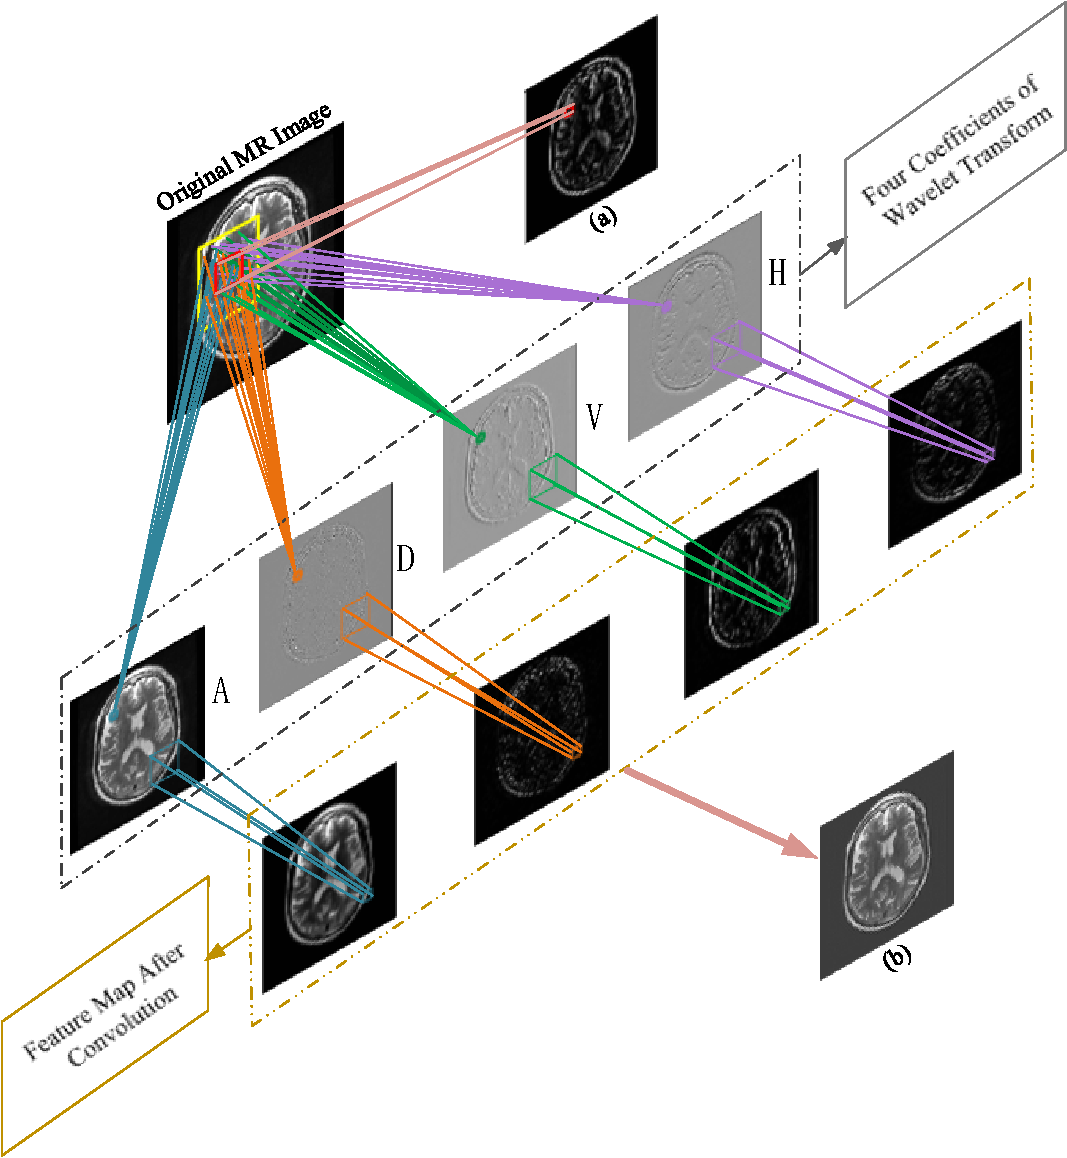
\includegraphics[width=0.8\linewidth]{figs/paper3nonLocalField2.pdf}
      \caption{卷积嵌入小波提取非局部感受野}\label{paper3nonLocalField2}
    \end{figure}
图\ref{paper3nonLocalField2}以一幅原始MRI为例的实现过程。根据新定义的卷积,首先通过小波变换生成四个系数分量(A:原始影像的近似表示,D:原始影像的对角边缘特征,V:垂直方向的奇异特征,H:水平方向的奇异特征)。然后对每个分量进行卷积,可得到四幅特征图。由于小波分解的四个系数表示不同的影像特征,因此在图\ref{paper3nonLocalField2}的原始MRI中,将它们堆叠后的区域用黄色框标记。初始卷积的局部感受野也用红框标记以供比较。根据小波变换理论,进一步的频域逐点更新将对小波变换中涉及的所有输入特征产生全局特征。当进行逆小波变换以获得最终的特征图(见图\ref{paper3nonLocalField2}(b))时,扩展的局部感受野进一步扩散到非局部感受野。并且,可以看到特征图影像非常接近原始影像,没有太多的信息损失。初始卷积的最终特征图如图\ref{paper3nonLocalField2}(a)所示,与原始影像有很大的不同,有很多信息丢失。

基于自定义的小波分解函数,本章提出了一个小波卷积单元,如图\ref{paper3framework}中黄色方块所示。它由四部分组成:编码器,WCU,解码器,全连接。WCU(wavelet convolution unit)是一个自定义的跨尺度信息提取模块,它利用小波分析和嵌入卷积来提取跨尺度信息。为了获得非局部的感受野,本章对单尺度小波分解系数进行卷积运算。此外,多尺度小波分解可以获得更全面的多尺度特征信息。此外,为了解决奇异点定位不准确的问题,本章将这些跨尺度特征融合到小波卷积单元中。本章的WCU如算法\ref{paper3algorithmWCU}所示。


\begin{algorithm}[ht]
\caption{Wavelet Convolution Unit}\label{paper3algorithmWCU}
\begin{algorithmic}[1]
\State {\textsc{WCU}}$~(X)$
\State \hspace{0.5cm}$W_s \gets$ SinScaT$~(X,~wave)$;
\State \hspace{0.5cm}$W_m \gets$ MulScaT$~(X,~wave)$;
\State \hspace{0.5cm}$W \gets$ Concatenate$~([W_s,~W_m],~1)$;
\State \hspace{0.5cm}$X_r \gets$ $\xi_{wav}~(W)$;
\State \hspace{0.5cm}\textbf{return} $X_r$;

\State \textbf{Function} {SinScaT}$~(X,~wave)$
\State \hspace{0.5cm}$C:\{c_i\}_{i=0}^3 \gets$ dwt$~(X,~wave)$;
\State \hspace{0.5cm}$\Hat{C}:\{\hat{c}_i\}_{i=0}^3 \gets$ $\xi_{wav}~({c}_0,~{c}_1,~{c}_2,~{c}_3)$;
\State \hspace{0.5cm}$\Gamma_s \gets$ idwt$~((\hat{c}_0,~\hat{c}_1,~\hat{c}_2,~\hat{c}_3),~wave)$;
\State \hspace{0.5cm}\textbf{return} $\Gamma_s$;

\State \textbf{Function} {MulScaT}$~(X,~wave)$
\State \hspace{0.5cm}$\Hat{C} \gets$  wavedec$~(X,~wave,~3)$;
\State \hspace{0.5cm}$\Gamma_{0,1} \gets$ idwt$~(\hat{c}_0,~\hat{c}_1,~wave)$;
\State \hspace{0.5cm}$\Gamma_{3,2} \gets$ idwt$~(\Gamma_{0,1},~\hat{c}_2,~wave)$;
\State \hspace{0.5cm}$\Gamma_m \gets$ idwt $~(\Gamma_{3,2},~\hat{c}_3,~wave)$;
\State \hspace{0.5cm}\textbf{return} $\Gamma_m$;
\end{algorithmic}
\label{alg1}
\end{algorithm}

\if 0
    \begin{figure}
      \centering
      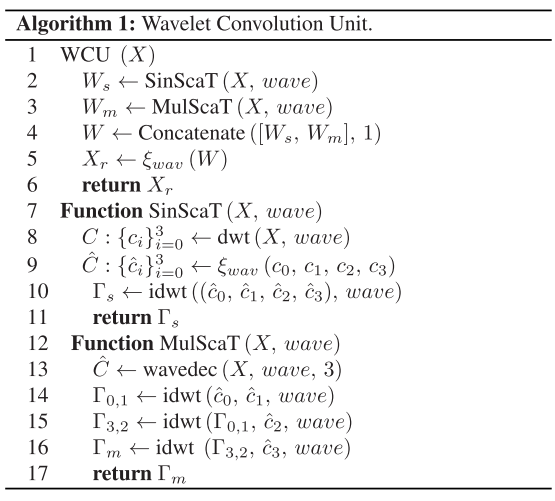
\includegraphics[width=0.75\linewidth]{figs/paper3Algorithm1WCU.png}
      \caption{WCU(Wavelet Convolution Unit)算法}\label{paper3algorithmWCU}
    \end{figure}
\fi
首先对影像进行单尺度分解,得到低频近似系数和三个(水平、垂直和对角)高频细节系数,并对每个系数应用$\xi$函数,然后对系数进行逆变换。在逆变换之前,先用$\xi$函数改变小波变换域的局部系数,可以选择性地扩大局部细节的分类,减少无用成分。同时将影像分解为三个尺度,根据不同尺度系数进行重构,得到变换后的特征图。最后,将两次重构的结果连接在一起,并再次应用$\xi$函数,以获得小波卷积单元的输出结果。在实验测试中,本章选择的小波基函数是Haar小波(一阶Daubechies小波),这是唯一直接适用于离散二维影像的不连续小波。Haar小波具有正交性和对称性。此外,在多尺度分解部分,本章设置了3尺度分解。在单尺度小波分解的卷积中,设置$size=1, stride=1, padding=0$在单尺度和多尺度组合的卷积中,设置$kernel size=3, stride=1, padding=1$。
    
    \begin{figure*}[t]
      \centering
      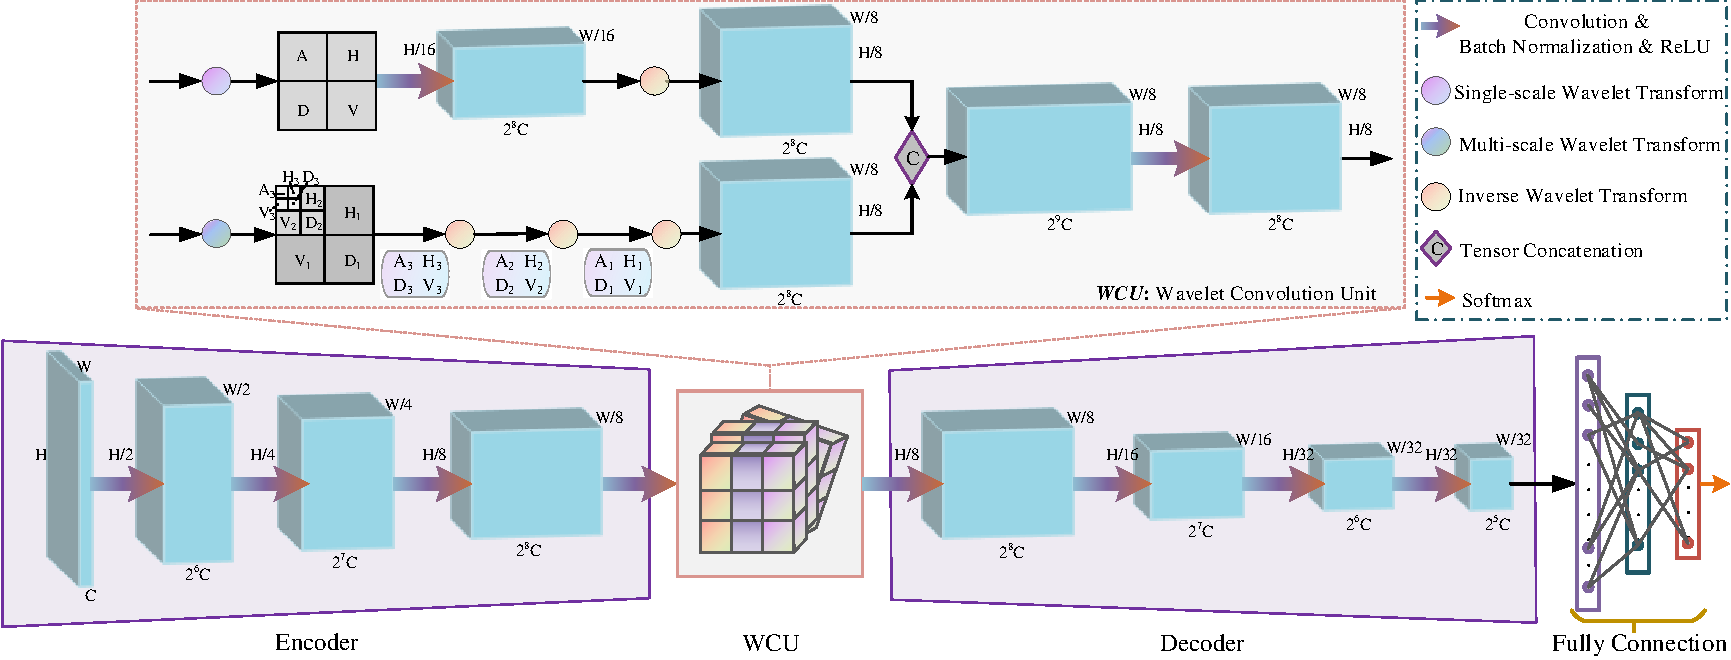
\includegraphics[width=0.9\linewidth]{figs/paper3framework.pdf}
      \caption{本节提出的小波卷积网络的框架图}\label{paper3framework}
    \end{figure*}


\subsection{细粒度多分类的网络结构}\label{paper3WCU-Net}
CNN作为深度学习中的一种典型网络结构,它由几层组成,包括但不限于卷积层、池化层、激活层和全连接层。本章方法的框架主要由四部分组成,包括编码,小波卷积单元,解码和全连接层,如图\ref{paper3framework}所示。为了有效地处理变长/短序列,使用编码和解码的思想。在编解码阶段,主要采用初级卷积运算来不断调整网络层的深度。在这两个过程中,使用了卷积层、BN和激活层的组合来提高网络模型的拟合能力。深度CNN的卷积层用于提取影像局部区域的尺度/位移不变特征。卷积层的主要好处是在同一特征图中共享权重,这减少了参数并导致模型的简单化。卷积层的不同层中的输入和输出通道的数量如图\ref{paper3framework}中蓝色框周围的值所示。在所有卷积层中,$kernel size=4, stride=2, padding=1$。卷积层后面是BN层,它本质上是一个归一化的网络层。

接着,将每个隐藏层神经元的输入逐步对接到非线性激活函数,最终归入该函数的值区间的极限饱和区域。将其设计为一般正态分布,其中,0为平均值,1为方差值。为了避免梯度消失,非线性函数被设计来处理输入特征。接下来是为模型引入激活层,以学习复杂的表示。为了提高收敛速度,本节中使用的激活函数(除了最终输出)是非线性激活函数ReLU。CNN的性能主要取决于层结构和滤波器集合,研究表明网络结构设计是提高CNN性能的有效途径\cite{liang2021cameranet}。本节基于小波的局部化和多分辨率特性,设计了一种小波卷积单元。最后一部分是全连接层。在前面的部分中处理的特征图已经变成了一个矢量,它不再是空间定位的。通过增加全连接层,可以发现卷积层中局部特征之间的非线性关系。本章使用了3层全连接,并通过softmax输出预测的类别。为了提高网络模型的泛化能力,在全连接前后采用了dropout方法,并将系数设置为0.5。在训练过程中,本章使用经典的交叉熵损失函数计算真实的标签和预测输出之间的损失。


\subsection{临床特征驱动型辅助分类}\label{paper3WCUNetClassify}

\subsubsection{临床特征驱动的脑影像数据}
众所周知,数据预处理一直是深度学习模型的重要步骤,尤其是在医学领域。DTI是MRI的一种特殊表现形式,是一种能有效观察和追踪白色纤维束的无创性方法。MRI主要用于AD和其他症状的诊断。一般来说,DTI能更好地反映脑部疾病的特征,有利于诊断。

在三维视图中,用对称矩阵的概念量化扩散各向异性的信号数据,定义为$D$,如等式(\ref{paper3dti})。其中,$D_{xx}$、 $D_{yy}$、 $D_{zz}$是沿着空间直角坐标系的$x$、$y$、$z$轴三个相互正交方向上传播的弥散系数。DTI表现为一个3$\times$3对称正定矩阵,它包含三个特征值($\lambda_{1}$, $\lambda_{2}$, $\lambda_{3}$)和相关的特征向量$V=(v_1, v_2, v_3)^T$。这3个特征向量分别指示了水分子扩散的三个主要方向,而与之对应的特征值则体现了水分子在这三个方向上的弥散强度。

\begin{equation}\label{paper3dti}
\begin{aligned}
D &=\left(\begin{array}{lll}
D_{xx} & D_{xy} & D_{xz} \\
D_{xy} & D_{yy} & D_{yz} \\
D_{xz} & D_{yz} & D_{zz}
\end{array}\right) & = V^T\left(\begin{array}{ccc}
\lambda_{1} & 0 & 0 \\
0 & \lambda_{2} & 0 \\
0 & 0 & \lambda_{3}
\end{array}\right)V.
\end{aligned}
\end{equation}

在本章的方法中,使用DTI的FA和MD指标($Ind_{FA}, Ind_{MD}$分别由式(\ref{paper3FA})和(\ref{paper3MD})表达),这两个指标可以使用FSL软件或脚本对DTI数据进行预处理获得。如图\ref{paper34classify}中黄色背景的方块所示。MD影像在第一行,第二行是FA影像。FA的值与白质内部髓鞘的完整性、纤维束的密集程度以及纤维排列的平行性呈正相关关系。因此,FA影像对脑内白质纤维结构的观察最为清晰,灰质边界明显。$Ind_{FA}$的计算公式如(\ref{paper3FA})所示。其中,$\bar{\lambda}$ 是三个特征值的平均值。MD反映了分子的整体扩散水平和阻力。MD仅反映了扩散的整体程度,而不涉及扩散的具体方向。$Ind_{MD}$越大,组织中包含的游离水分子越多。$Ind_{MD}$的计算公式如(\ref{paper3MD})所示。$Tr(D)$是$D$的迹,它是一个矩阵不变量。

 \begin{equation}\label{paper3FA}
Ind_{FA}=\sqrt{\frac{\sum_{i=1}^{3}3\left(\lambda_{i}-\bar{\lambda}\right)^{2}}{\sum_{i=1}^{3}2\lambda_{i}^{2}}},
\end{equation}
\begin{equation}\label{paper3MD}
Ind_{MD}=Tr(D)/3=\left(D_{xx}+D_{yy}+D_{zz}\right)/{3}.
\end{equation}


\subsubsection{细粒度与多分类的技术路线}\label{4.3.3.2}
本节建立了一个新的框架,通过WCU-Net实现AD的细粒度和多分类。对于二、三和四分类框架通用,在实验装置中,只有它们的输入和输出不同。如图\ref{paper34classify}所示,该框架包括三个部分:数据输入,编码器、WCU、解码器、FC和激活函数的网络架构,以及类别预测的输出。在第一部分中,对DTI数据进行了预处理。FSL(https://fsl.fmrib.ox.ac.UK/fsl/fslwiki/Fsl Installation/Linux)工具对原始DTI数据进行b0影像提取、剥脑、涡流校正、张量计算等预处理操作。从所获得的张量指数中选择FA和MD作为输入的数据。在第二部分中,依次输入4个类别(AD,NC,EMCI,LMCI)的FA和MD,并分别通过编码器,WCU,解码器,FC和激活函数(Softmax)。在这一部分中,主要对WCU中的流程进行了扩展和展示。WCU采用自定义的小波卷积单元,结合单尺度小波分解和多尺度小波分解的特点,获得完整的跨尺度特性。最后一部分是网络的预测输出,其将概率分布转换为标签数据。最终的预测类别取决于具有最高概率的类别。
    \begin{figure*}[ht]
      \centering
      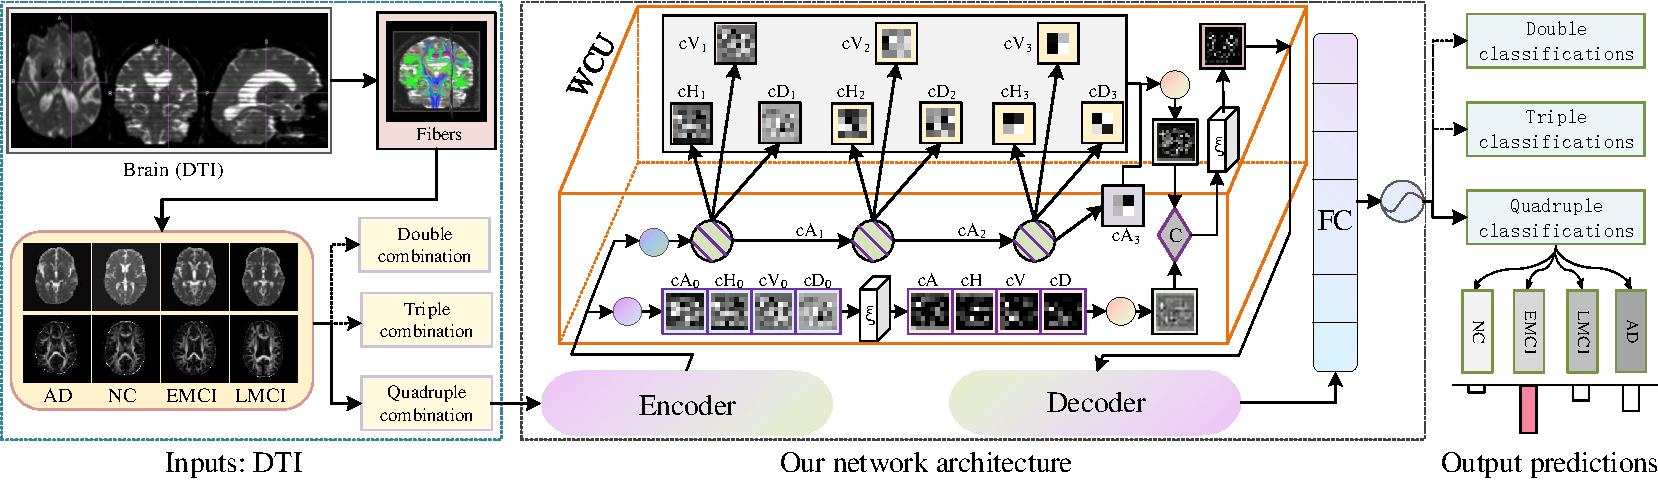
\includegraphics[width=0.9\linewidth]{figs/paper34classify.pdf}
      \caption{WCU-Net应用于细粒度多分类任务中的具体步骤} \label{paper34classify}
    \end{figure*}


%\subsubsection{预训练模型参与应用的分析}
CNN是深度智能系统中最常用于检测AD的网络,一些研究倾向于设计CNN的结构\cite{bringas2020alzheimer}。经典的网络结构,如ResNet,DenseNet,SqueezeNet,Inception,AlexNet,VGGNet和GoogLeNet,已成功应用于影像分类任务\cite{ananda2021classification},这有助于权重初始化过程。在本节中,利用这7个经典的网络模型初始化本章提出的网络结构权重。表\ref{paper3withPretrained}列出了WCU-Net与预训练CNN的分类准确度,其中,D-1: AD vs. NC, D-4: AD vs. EMCI, D-5: AD vs. LMCI, D-6: NC vs. EMCI, D-7: NC vs. LMCI, D-8: EMCI vs. LMCI, T-2: AD vs. EMCI vs. LMCI, T-3: NC vs. EMCI vs. LMCI, QC: AD vs. NC vs. EMCI vs. LMCI),2-9列的每一列表示不同的网络模型参与的应用(Net\_1: ResNet101, Net\_2: DenseNet161, Net\_3: SqueezeNet1\_1, Net\_4: Inception\_v3, Net\_5: AlexNet, Net\_6: VGG13, Net\_7: GoogLeNet, Net\_8:w/o pretrained CNNs。在权重初始化过程中是否采用预训练CNNs模型的分类准确率也列在最后一列以供比较。从表\ref{paper3withPretrained}可以看出,每个预训练模型都能在一定程度上提高2-4种组合分类的准确率,在第2-8列用红色或蓝色值标记。特别是对于细粒度的NC vs. EMCI和NC vs. LMCI二分类,预训练的效果明显。总之,九种组合分类的最高准确度值分别达到0.9920,0.9730,0.9611,0.9870,0.9611,0.9900,0.9636和0.9379,其中AD与NC,AD与EMCI和AD与LMCI与EMCI与NC的最佳分类准确度由WCU-Net得到,无预训练CNNs模型参与。而在本节中,所提出的方法则是使用未经预训练网络初始化参数的WCU-Net,并获得的结果与现有的AD分类方法进行比较。

\begin{table}[ht]
 \centering
\caption{权重初始化过程中是否采用预训练模型的精度比较}
%\small
\begin{tabular}{ccccccccc}
\toprule
Class   &  Net\_1 &  Net\_2   &  Net\_3 &Net\_4   & Net\_5  & Net\_6  &  Net\_7   &\textbf{Net\_8}    \\ \midrule
D-1 & 0.9840 & 0.9890 & 0.9790  & 0.9710 & 0.9701 & 0.9850 & 0.9890 &\textcolor{red}{{0.9920}}  \\
D-4 & 0.9630 & 0.9550 & 0.9690 & 0.9670  & 0.9500 & 0.9480 & 0.9680 &\textcolor{red}{{0.9730}}  \\
D-5 & 0.9533 & 0.9556 & 0.9533 & 0.9511 & 0.9478 & \textcolor{red}{{0.9611}} & 0.9522 & 0.9578    \\
D-6  & \textcolor{green}{{0.9750}}           & \textcolor{green}{{0.9720}}
& \textcolor{green}{{0.9650}}
& \textcolor{green}{{0.9710}}
& \textcolor{green}{{0.9690}}
& \textcolor{red}{{0.9870}}
& \textcolor{green}{{0.9700}}
& 0.9500    \\
D-7 & \textcolor{red}{{0.9611}}
& \textcolor{green}{{0.9533}}
& \textcolor{green}{{0.9456}}
& \textcolor{green}{{0.9489}}
& \textcolor{green}{{0.9567}}
& 0.9089
& \textcolor{green}{{0.9590}}
& 0.9400    \\
D-8
& \textcolor{green}{{0.9800}}
& \textcolor{green}{{0.9800}}
& 0.9722
& \textcolor{green}{{0.9833}}
& 0.9644
& 0.9778
& \textcolor{red}{{0.9900}}
& 0.9789\\
T-2
& 0.9350
& \textcolor{green}{{0.9586}}
& 0.9490
& 0.9521
& \textcolor{green}{{0.9600}}
& \textcolor{green}{{0.9586}}
& \textcolor{red}{{0.9636}}
& 0.9571\\
T-3
& 0.9257
& 0.9243
& 0.9464
& \textcolor{red}{{0.9833}}
& 0.9193
& 0.9407
& 0.9429
& 0.9507
\\
QC
& 0.9353
& 0.9168
& 0.9284
& 0.9068
& 0.9358
& 0.9337
& 0.9053
& \textcolor{red}{{0.9379}}
\\ \bottomrule
\end{tabular}
\label{paper3withPretrained}
\end{table}


\section{细粒度多分类的实验}\label{chapter4.4}
\subsection{实验验证的数据说明}
本节中使用的数据来自ADNI(www.adni-info.org)。由于每个类别的数据量不相等,并且数据的总数不足以训练深度学习模型,因此使用数据扩大来增加每个少数类别的样本数量。另外,医学影像可视化后是灰度影像,为了不对影像造成较大的改变,数据增强方法主要是通过加入随机噪声和亮度进行扩大。为了增加数据的大小,本章将使用数据增强来扩展所获得的数据。数据增强的方法与文献\cite{Fangmeie2022}一致,数据增强后的情况见表\ref{paper3sourceData}。

\begin{table}[ht]
\centering
\caption{增强前后的数据集详情}\label{paper3sourceData}
\begin{tabular}{ccccc}
\hline
\normalsize
Diagnosis      & \multicolumn{1}{c}{AD}      & \multicolumn{1}{c}{EMCI}      & \multicolumn{1}{c}{LMCI}     & \multicolumn{1}{c}{NC}        \\ \hline
Age            & \multicolumn{1}{c}{75.23}   & \multicolumn{1}{c}{73.95}     & \multicolumn{1}{c}{73.45}    & \multicolumn{1}{c}{74.52}     \\
Gender(M/F)   & \multicolumn{1}{c}{99 / 54} & \multicolumn{1}{c}{225 / 138} & \multicolumn{1}{c}{108 / 59} & \multicolumn{1}{c}{110 / 109} \\
Subjects       & \multicolumn{1}{c}{153}     & \multicolumn{1}{c}{363}       & \multicolumn{1}{c}{167}      & \multicolumn{1}{c}{219}       \\
MMSE           & \multicolumn{1}{c}{18-27}   & \multicolumn{1}{c}{24-30}     & \multicolumn{1}{c}{24-30}    & \multicolumn{1}{c}{25-30}     \\ \hline\hline
Train data & \multicolumn{1}{c}{9273}    & \multicolumn{1}{c}{9748}      & \multicolumn{1}{c}{10154}    & \multicolumn{1}{c}{10113}     \\
Valid data & \multicolumn{1}{c}{2100}    & \multicolumn{1}{c}{2088}      & \multicolumn{1}{c}{2100}     & \multicolumn{1}{c}{2200}      \\
Test data   & \multicolumn{1}{c}{500}     & \multicolumn{1}{c}{400}       & \multicolumn{1}{c}{500}      & \multicolumn{1}{c}{500}       \\ \hline
\end{tabular}
\end{table}

DTI是MRI的一种特殊形式,但其获取比MRI困难。DTI可以捕捉脑内的白色物质束和灰质束,并通过测量活体组织内水分子的扩散来工作。由于扩散张量是一个对称的$3 \times3$矩阵,它可以用它的特征值($\lambda_{i}$)和特征向量($V_{i}$)来描述,然后使用特征值和特征向量来处理标量指数。两个主要的扩散指数(FA和MD)是基于本征值和代表的扩散过程的幅度。年龄是AD的主要危险因素,因此选择年龄在73-76岁之间且认知功能评分差异显著的人群(AD:18-27,EMCI/LMCI:24-30,NC:25-30)进行研究分析。所下载的数据集来自902个样本,分为四类:153个AD患者,167个LMCI,363个EMCI和219个NC。选择DTI数据集作为模型的训练集、验证集和测试集,数量如表\ref{paper3sourceData}所示。

\subsection{实验验证的参数说明}
在网络训练过程中,影像的大小为128 × 128。在训练过程中,初始学习率为0.001,40个epoch,批量大小为32,使用批量归一化。优化函数是SGD,动量的值为0.85。此外,实施了一种动态调整的学习率策略,每隔8个训练周期将学习率降低至初始值的10\%。本章使用Python 3.8.12和Pytorch 1.10.2版本,CUDA版本为10.2,系统为Tesla T4 16 G RAM 64 GNU/Linux x86。

\subsection{早期细粒度分类应用}
临床研究表明,AD的细粒度分型具有重要意义。关于AD的分类有很多研究,然而,大多数现有的方法局限于粗粒度的二分类,即,AD vs. NC、AD vs. MCI和MCI vs. NC。一些方法实现了粗粒度的三分类,即,AD与NC与MCI分类。近年来,一些学者对MCI进行了进一步的细粒度分类。早期很少有学者利用DTI数据做细粒度的二分类\cite{prasad2015brain, 2020Convolutional},其较高的准确率为0.81。一些学者使用MRI数据对AD进行了细粒度的四分类。Ashburner和Friston\cite{ashburner2000voxel}、Zhang等人\cite{zhang2016detecting}和Liu等人\cite{liu2018joint}提出应用于AD细粒度四分类并使用MRI数据的方法,但准确性较低。也有一些方法使用MRI数据应用于三分类和四分类,可以获得更好的性能。例如,在\cite{sorensen2018ensemble}中,三分类准确率可以达到68.8\%,四分类准确率可以达到59.1\%。然而,三分类是AD vs NC vs(EMCI+LMEC),这与传统的粗粒度三分类相似。在文献\cite{dimitriadis2018random}中四分类的准确率可达61.9\%。Basaia等\cite{2018Automated}提出了基于CNN的MRI数据MCI细粒度分类方法,实现了AD、LMCI、EMCI、NC六种组合双分类。Fang等人\cite{Fangmeie2022}提出了一种通过二次迁移学习的细粒度方法,提高了5种细粒度二分类的准确性。目前,De和Chowdhury\cite{de2021dti}实现了细粒度的四分类,精度为0.926。

     \begin{figure*}[ht]
      \centering
      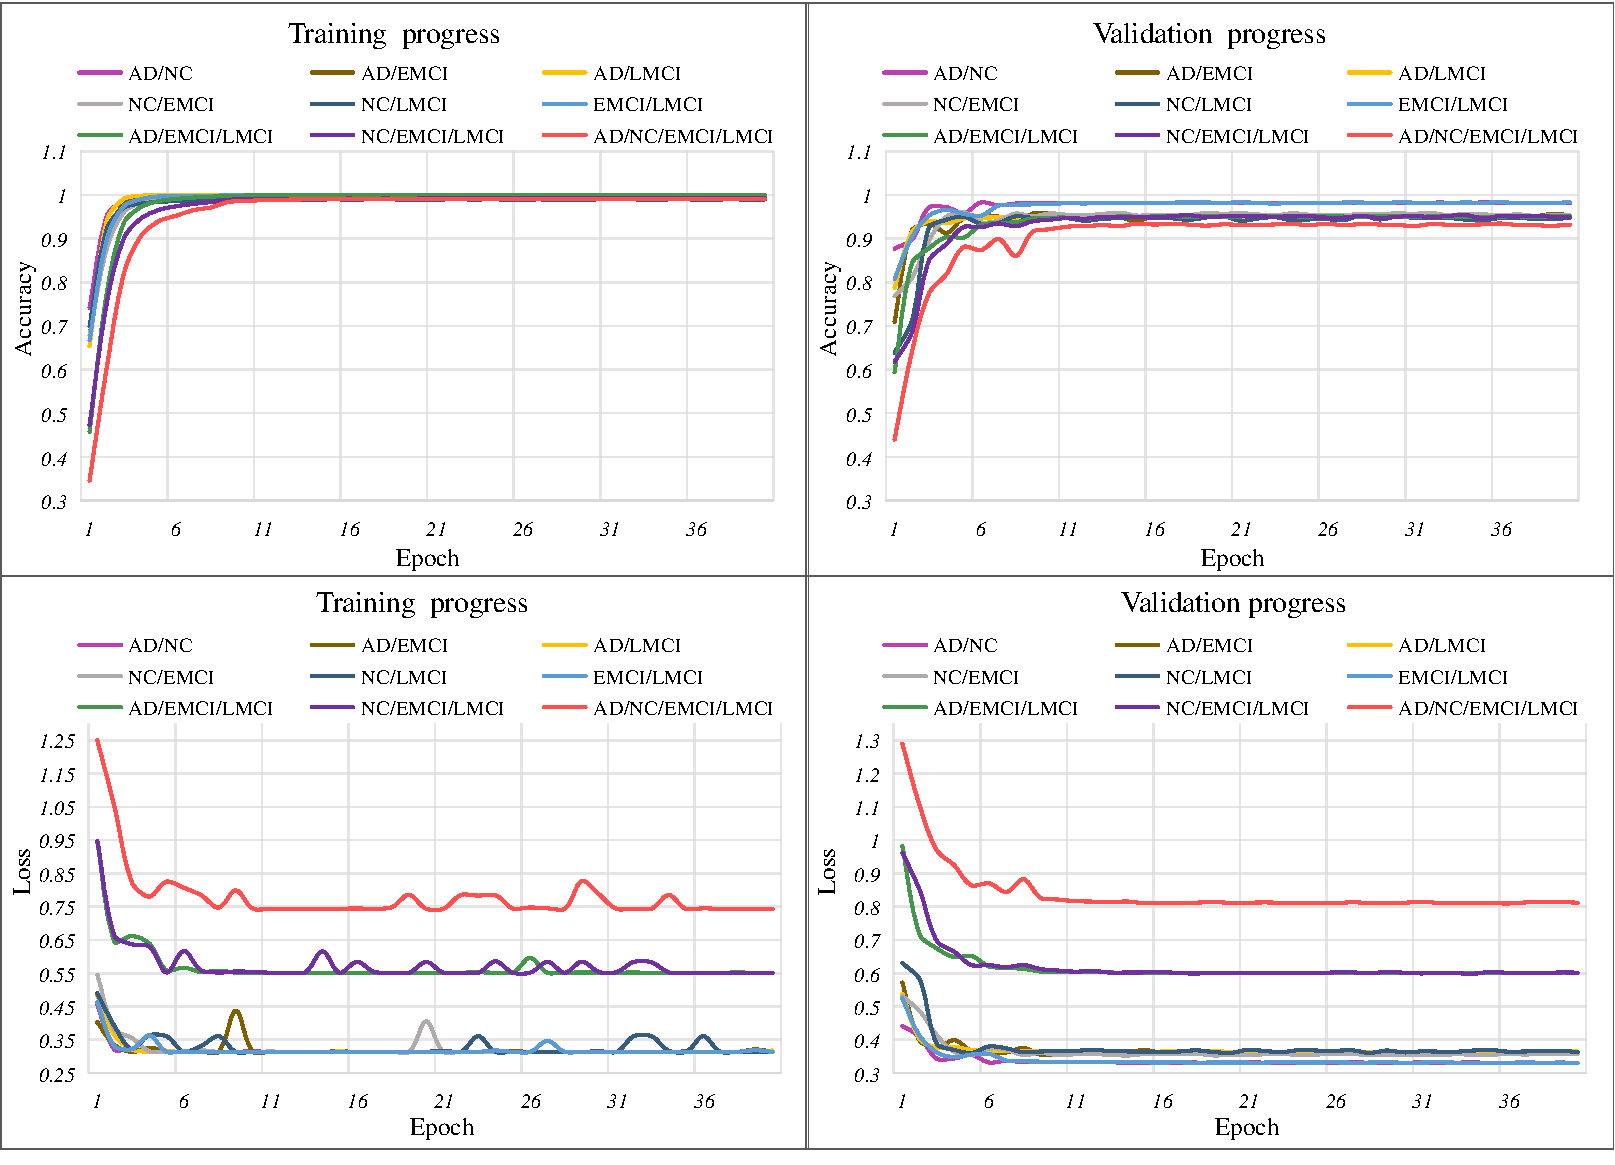
\includegraphics[width=0.9\linewidth]{figs/paper3lossandaccuracy.pdf}
      \caption{准确度曲线和损失曲线}\label{paper3curves}
    \end{figure*}
    
在本节中,为了便于尽可能准确地诊断AD分类,展开了12种组合分类,包括4种粗粒度分类和8种细粒度分类,如表\ref{paper3accuracy1}和\ref{paper3fine_classify}的所示。本章提出的方法是首次出现两种细粒度的三分类(AD vs. LMCI vs. EMCI和NC vs. LMCI vs. EMCI)。
表\ref{paper3fine_classify}列出了本章提出的方法对AD与NC分类以及8种粒度多分类的准确性。为便于比较,表\ref{paper3fine_classify}还列出了现有细粒度分类方法的准确性。可以观察到,对于实现的6种二分类,本章提出的方法的准确性比现有的方法\cite{2018Automated,Fangmeie2022}要好得多。对于细粒度的四分类,本章提出的方法准确率为0.9379,也比\cite{de2021dti}提高了1.19\%,首次实现了细粒度的三分类,其中AD vs. EMCI vs. LMCI、NC vs. EMCI vs. LMCI的准确度分别达到0.9571和0.9507。

图\ref{paper3curves}中的第一行显示了在没有预训练的网络模型作为初始化权重参数的情况下,所提出的方法的预测精度曲线分布,并且在训练阶段和验证阶段之间的分布存在一定的偏差。在训练过程中,准确率曲线没有波动,并且随着训练时期的增加,在不同分类组合中的准确率更接近于1。在验证过程中,1-8轮出现了小范围的振荡,但总体上升趋势是正确的。在验证过程中,参数不断更新。随着轮数的增加,AD vs. NC和EMCI vs. LMCI分类的准确率接近1,四分类的准确率稍低,但也在0.9-1之间。在其他数据组合分类的情况下,精度也稳定在第11轮。图\ref{paper3curves}中的第二行显示了训练和验证阶段的损失曲线。二分类的损失较小,而四分类的损失相对较大。而训练和验证过程中的损失明显减少,并趋于稳定。因此,表明本节提出的网络模型具有良好的泛化性能。

    \begin{figure*}[ht]
      \centering
      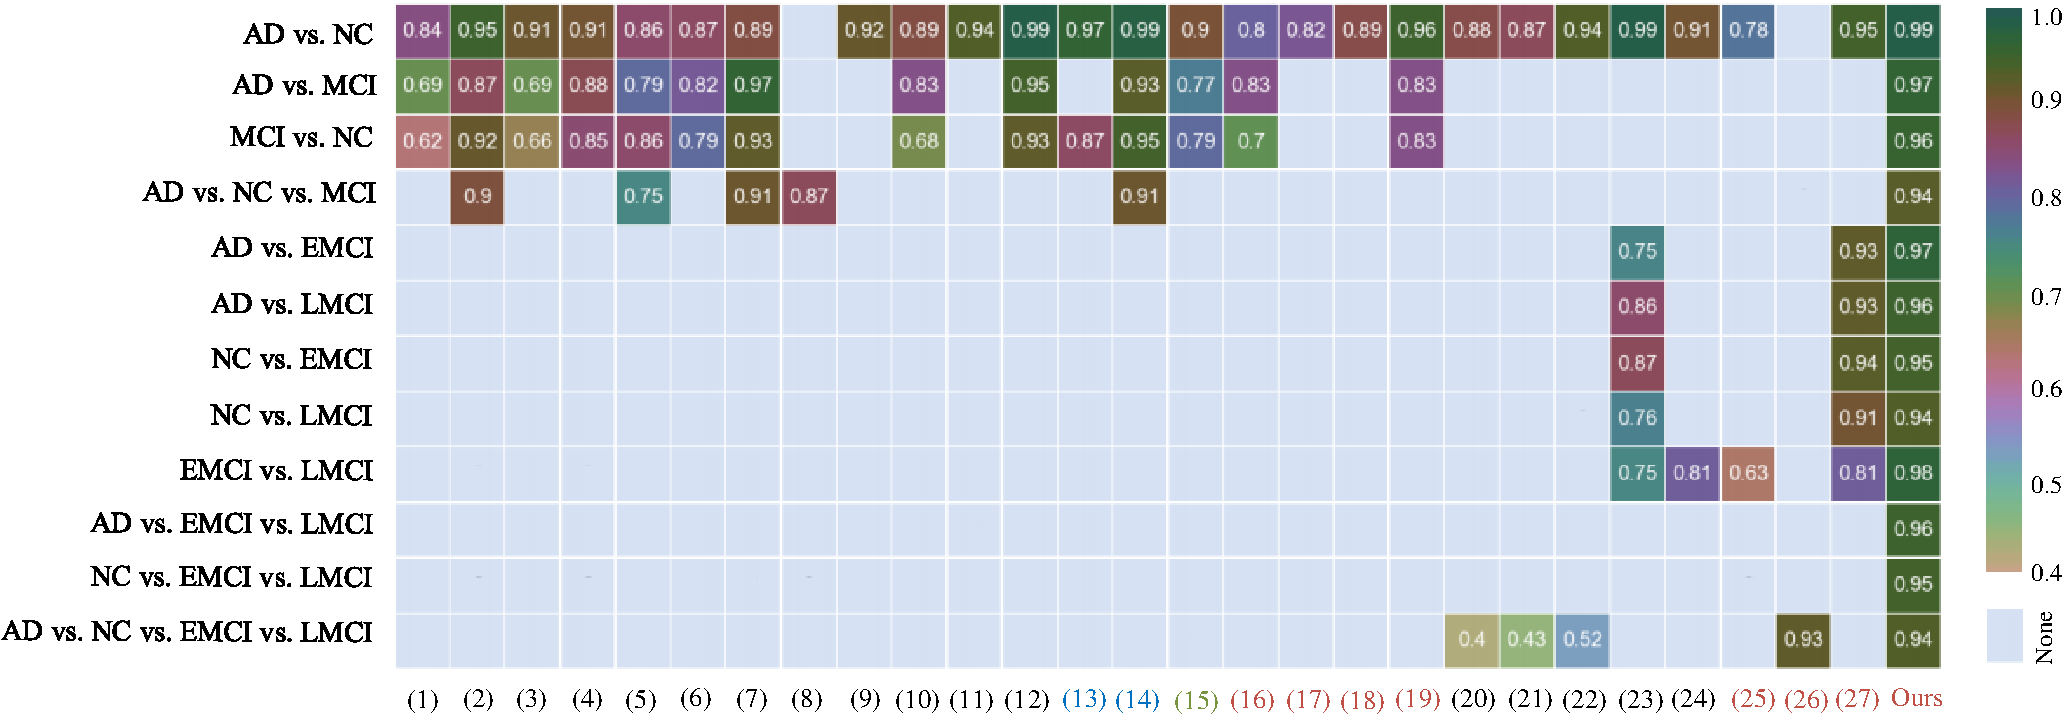
\includegraphics[width=0.9\linewidth]{figs/paper3rlt20230306-2.pdf}
      \caption{各种粗粒度和细粒度AD分类方法精度比较的热力图}\label{paper3heatmap}
    \end{figure*}
    
\subsection{多类别分类应用分析}
图\ref{paper3heatmap}显示了本文所涉及的所有粗粒度和细粒度AD分类的准确性比较的热力图。图中的小矩阵单元颜色越深,其相应方法的准确度越高。淡蓝色单元格表示没有相应的分类工作。大面积的浅蓝色单元表明,大多数现有的方法只关注于少数组合分类。但本章提出的方法实现了所有12种分类,对于所有细粒度分类都具有较高精度,为以后该领域的研究工作提供了完整的参考。图中横轴上颜色相同的数字表示这些方法使用的数据模态是相同的。红色、蓝色、绿色和黑色分别对应于DTI、MRI+PET、MRI+DTI和MRI。(1)-(27)列分别指下列参考文献中提出的不同方法:Ben Ahmed et al. \cite{ahmed2015alzheimer}, Payan and Montana \cite{payan2015predicting}, Aderghal et al. \cite{aderghal2017classification}, Yang et al. \cite{yang2017active}, Xiao et al. \cite{xiao2017brain}, Madusanka et al. \cite{madusanka2019alzheimer}, Bi et al. \cite{bi2020computer}, Duc et al. \cite{duc20203d}, Xing et al. \cite{xing2020dynamic}, Pan et al. \cite{pan2020early}, Ebrahimi and Luo \cite{ebrahimi2021convolutional}, Liu et al. \cite{liu2022diagnosis}, Lei et al. \cite{lei2016discriminative}, Vu et al. \cite{vu2018non}, Ben Ahmed et al. \cite{ahmed2017recognition}, Ebadi et al. \cite{ebadi2017ensemble}, Qu et al. \cite{qu2021ai4ad}, Lella et al. \cite{lella2021ensemble}, Bigham et al. \cite{bigham2022features}, Ashburner and Friston \cite{ashburner2000voxel}, Zhang et al. \cite{zhang2016detecting}, Liu et al. \cite{liu2018joint}, Basaia et al. \cite{2018Automated}, Wen et al. \cite{2020Convolutional}, Prasad et al. \cite{prasad2015brain}, De and Chowdhury \cite{de2021dti}, Fang et al. \cite{Fangmeie2022}。从这张热图中,可以得出以下结论:
\begin{itemize}
    \item 大多数方法只能实现粗粒度的分类。一些方法实现了一种或几种细粒度分类。本章的方法实现了所有12种的组合分类,而且只有本章的方法实现了细粒度的三分类。
    \item 大多数方法对于不同类别组合的精度不稳定,甚至存在许多精度小于0.70。本章的方法实现了稳定的分类且精度高于0.935的有12种组合分类。

\end{itemize}
    
  \begin{figure}[ht]
      \centering
      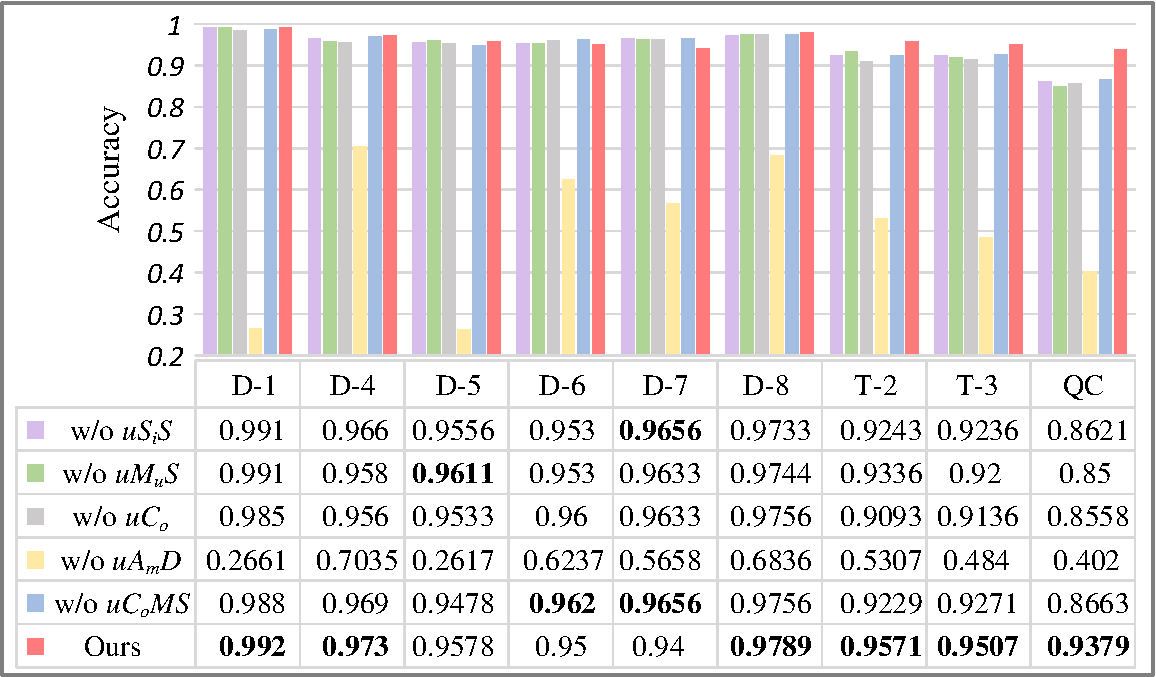
\includegraphics[width=0.9\linewidth]{figs/paper3ablation4.pdf}
      \caption{本章提出的方法的消融实验}\label{paper3ablation}
    \end{figure}  
关于AD分类的研究工作似乎很多,但他们通常专注于不同的数据模态和类别的组合,各种方法之间的可比性不是很强。本章方法实现了所有12种粗粒度和细粒度分类,具有较高的准确率,为后续基于DTI数据的AD分类研究提供了一个合适的参考标准。不过,有一点需要特别说明。在本章中,主要集中在DL方法的准确性,但忽略了神经科学的部分,潜在的目标对的ROI可以关联到AD的不同阶段。实际上,这对于基于神经科学的疾病研究和基于深度学习方法的智能辅助诊断的可解释性非常重要。在未来的研究中,将神经科学与人工智能方法更深入地结合将是一个有意义的研究方向。

\subsection{细粒度多分类的消融实验}

如第\ref{chapter4:WCU-net}节所述,本章的方法的最佳性能主要取决于单尺度小波分解($uS_{i}S$)、多尺度小波变换($uM_{u}S$)、$\xi$函数运算($uC_{o}$)和数据扩增$uA_{m}D$。为了进一步证明这四个部分的有效性,本章设计了五组方法进行消融实验,即,缺少$uS_{i}S$、缺少$uM_{u}S$、缺少$uC_{o}$、缺少$ uA_{m}D$和缺少$uC_{o}MS$(缺少$uM_{u}S$和$uC_{o}$)。所有的实验结果都显示在图\ref{paper3ablation}中,与本章的方法进行比较。表格中的每行表示的是不同的方法,每列代表不同的组合分类,各组合同章节\ref{4.3.3.2}定义的相同。从图\ref{paper3ablation}可以发现,数据扩增至关重要,其他部分对于细粒度分类也很重要。特别是在细粒度的四分类中,各组件的结合使用,分类精度有了明显的提高。



\section{本章小结}\label{chapter4.5}
本章提出了一种新的网络WCU-Net,它在小波卷积单元中结合了单尺度和多尺度变换。该策略不仅获得了非局部感受野,而且实现了跨尺度信息融合。然后将WCU-Net成功地应用于AD细粒度和多分类中,并达到SOTA精度。细粒度分类对于认知障碍的准确诊断和正确治疗具有重要意义。细粒度分类特别是细粒度的四分类准确率还有待进一步提高。后续将会尝试在AD的更多分期中应用WCU-Net,以及基于医学影像的不同性质疾病的分类,并进行更多研究。

%%% Local Variables:
%%% mode: latex
%%% TeX-master: "../main"
%%% End:

% !TEX root = ../main.tex
\chapter{帕金森疾病的智能辅助预测} 
\label{chapter:pdPrediction}
%帕金森病(PD)作为神经运动功能障碍及神经组织退行性变疾病中最为普遍和常见的一种,目前面临的主要挑战之一是许多患者在临床确诊时已经处于疾病的中晚期,导致错过了进行最佳临床治疗的黄金时期\cite{de2019prognosis,papagno2018cognitive}。因此,需寻找更快速、准确、和有效的筛查方法,以便在早期阶段诊断PD患者。这一挑战促使了对机器学习(ML)在PD分类预测中的研究,ML技术的发展为智能辅助诊断与健康测评提供了智能决策技术,有望解决特殊情况下的误诊或无法确诊的问题。
%在当前的研究趋势中,对于PD预测的关键问题之一是如何克服临床诊断的滞后性,使患者能够更早地接受有效的治疗。多模态数据融合成为研究的热点之一,通过整合临床数据、基因表达数据和影像数据等不同类型的信息,有望提供更全面和准确的PD分类预测。

%在第\ref{chapter5.1:pdPredictReview}节中基于机器学习的智能辅助PD分类预测进行了综述,突出了机器学习技术在提高PD智能辅助诊断与健康测评方面的潜力。ML模型的发展不仅有助于解决特殊情况下的误诊或无法确诊的问题,而且通过挖掘海量数据中的潜在规律,构建了一套相应规律的决策模型,为早期诊断提供了新的可能性。
%在第\ref{chapter5.2:pdCMF-Net}节中,我们提出了一种跨模态数据融合的机器学习方法(CMFP),通过综合利用基线DTI和临床特征数据,提出了一种智能辅助PD进展预测的创新方法。该方法的重要性在于通过纵向数据研究方法,结合机器学习,建立了早期PD基线DTI及临床特征的疾病进展模型。研究结果表明,跨模态的数据融合能够显著提高单模态预测的精确度,尤其在传统机器学习方法的应用中。这一发现为未来的PD研究提供了新的思路,强调了跨模态数据融合在提高预测性能方面的潜在优势。

PD的发生机制因素除复杂性外,还涵盖了遗传背景、环境暴露及生活习惯等多个层次的交织影响。其中,$\alpha$-突触核蛋白聚合现象是其生物学标识的核心组成部分。现有多模态影像整合技术在探究医学信息与影像特征深层次相关性方面存在不充分的问题,这在一定程度上限制了其在脑部疾病诊断中的表现力。
为了提升对PD等多种脑疾病的精确诊断能力,亟需引入跨模态数据集成分析的方法。
机器学习(ML)技术的进步为智能辅助诊断与健康评估提供了智能的决策支持,有望应对特殊情况下的误诊或难以确诊的挑战。第\ref{chapter5.1:pdPredictReview}节综述了ML的智能辅助PD分类预测方法\cite{jyWen}。ML模型通过挖掘大量数据中的隐藏规律,为早期辅助诊断提供了新的机会。
在第\ref{chapter5.2:pdCMF-Net}节中,提出了一种跨模态数据融合的ML方法(CMFP),它是通过综合DTI和临床数据的一种PD早期进展预测的新方法,可显著提高单模态预测的精确度。

\section{引言}
%帕金森病(PD)是一种以神经运动功能障碍和神经组织退行性变为特征的常见疾病。目前,我们面临的一个主要问题是,许多患者在确诊时已经进入疾病的中晚期,从而错过了最佳的治疗时机\cite{de2019prognosis,papagno2018cognitive}。为了解决这个问题,我们需要寻找更快速、更准确、更有效的筛查方法,以便能够及早地诊断出PD患者。这样做可以帮助我们更早地开始治疗,从而可能改善患者的预后和生活质量。

PD 是一种常见的神经系统疾病,主要影响人类的神经系统和运动控制\cite{2020Comparison},表现为静止时的颤抖、动作缓慢、身体活动受限以及平衡失调\cite{ameiPhdthesis}。PD随时间缓慢恶化,诊断依赖于患者的临床症状;肢体功能障碍和非运动症状不仅损害生活品质,还与较高死亡率相关,故早期预测和及时治疗至关重要\cite{agosta2015propagation}。至今为止,尚未发现能够准确反映PD的疾病进程的临床数据或生物指标\cite{ameiPhdthesis}。而且,对临床效果的评估往往需要较长的时间,且其结果易受到患者当时健康状况的影响而发生变化\cite{ameiPhdthesis}。标准的MRI能够展现清晰的组织差异,但在诊断疑似PD患者方面,它的主要价值在于帮助排除其他脑部疾病,而不是直接用来确认是否为PD\cite{post2008clinical}。PD 是一个异质性疾病,根据起病的年龄、临床表现及进展的快慢可以被分成不同的亚型\cite{thenganatt2014parkinson,rajput2009course}。PD疾病的发展会随着时间的演变而发生不同的变化,一些患者病情会保持稳定,而一些则进展为帕金森病痴呆(PDD)。因此,有必要预测PD疾病的进展。

研究发现,白质微观结构的变化在皮层神经元显著退化前就已发生,且这种变化未必与灰质体积减少相关\cite{ameiPhdthesis}。通过使用扩散张量成像(DTI)技术,研究者能够监测到帕金森病患者的大脑白质损伤,并发现这些损伤的程度与患者接下来一年中运动能力和认知功能的改变有着紧密的联系\cite{ameiPhdthesis,schwarz2013diffusion}。最新研究运用DTI技术揭示,在早期PD患者中,全脑体素分析指出胼胝体的分数各向异性(FA)和平均弥散度(MD)出现了明显的变化,特别是在膝部和压部区域更为显著\cite{amandola2022longitudinal}。研究还发现,胼胝体FA值的降低与大脑广泛皮质及皮质下区域的FA和MD值降低存在相关性\cite{amandola2022longitudinal}。进行多元回归分析后,结果表明在研究的起始点及两年后的跟进中,患者的运动刚性程度与胼胝体的FA值之间存在显著的负向关联,且这种关联在胼胝体前部区域最为突出。这些发现提示研究者们,在PD的早期阶段,胼胝体的微观结构变异可能是一个有用的生物标志物,用于监测运动刚性症状及其疾病进程的变化\cite{amandola2022longitudinal}。

\begin{table}[htbp]
\centering
\caption{基于机器学习技术在PD某一时刻智能辅助预测的相关工作}
\label{paper4MLpredictJt}
\small
\begin{tabular}{p{1.8cm}<{\centering}p{3.2cm}<{\centering}p{3.4cm}<{\centering}p{1.35cm}<{\centering}p{1.35cm}<{\centering}}
%\begin{tabular}{cccccc}
\hline 
\multicolumn{1}{c}{文献}  &方法    &数据及来源 &ACC(\%) &AUC(\%)  \\ \hline
文献\cite{sivaranjini2020deep}    &Transfer Learning (AlexNet)  &PMI 中的 MRI  &88.90  & -  \\ \\
文献\cite{martinez2018convolutional}   &Lenet 和Alexnet  &PPMI 中的 FP-CIT SPECT  &94.10  &98.40   \\ \\
文献\cite{kim2018artificial}    &Transfer Learning (Inception V3)  &PPMI 中的 SPECT  & -  &87.00   \\ \\
文献\cite{castillo2018robust}    &SVM和KNN的集成分类  &PPMI 中的 SPECT 和多种异质生物标志物
(CSF,Plasma,RNA和 Serum)  &96.00  & -   \\ \\
文献\cite{al2021feature}    &RF、XGBT和CatBoost的集成分类  &UCI 库中的声学特征  &86.25  & -   \\ \\
文献\cite{almeida2019detecting}   &KNN,MLP,OPF 和 SVM  &文献\cite{vaiciukynas2017detecting}中的发音与语言数据  &94.55  &87.00   \\ \\
文献\cite{nahar2021feature}    &GBT,XGBT,Bagging 和ExtraTree  &UCI 库中的声学特征  &82.35  & -   \\ \\
文献\cite{patra2019prediction}    &DT,LR和KNN的集成分类  &UCI 库中的声学特征  &84.59  & -   \\ \\
文献\cite{wang2020early}  &文献\cite{wang2020early}中提出的一种新颖的深度
学习方法  &PPMI中的REM,CSF、嗅觉丧失和SPECT数
据  &96.45  & -   \\ \\
文献\cite{prashanth2016high}     &NB,SVM,Boosting 和RF  &PPMI 中的睡眠行为障碍、CSF、嗅觉丧失和
DAT 数据  &96.40  &98.88   \\ \\
文献\cite{grover2018predicting}   &DNN  &UCI 库中的声学特征  &81.67  & -   \\  \\
文献\cite{masud2021crowd}   &文献\cite{masud2021crowd}中提出的一种新颖的深度
学习方法(CROWD)  &UCI 库中的声学特征  &96.00  & -   \\ \\
文献\cite{pahuja2022deep}    &CNN  &PPMI 中的 MRI,SPECT 和CSF  &93.33  & -   \\  \hline

\end{tabular}
\end{table}

%帕金森病是一种慢性退行性疾病,主要影响人类的神经系统和运动控制\cite{2020Comparison}。虽然PD的主要症状是运动障碍,如僵硬,但随着PD的进展,极有可能出现非运动症状,如抑郁或认知障碍\cite{2020Development}。随着人口老龄化的增加,帕金森病患者也在迅速增加,因此,用于评估和跟踪帕金森病的远程监测和远程诊断设备的进展已变得越来越重要\cite{2020Optimized,2005Fluorodopa}。Raval等人开发了一个模型,使用步态和姿势稳定性的临床测量和生物力学测量来预测个人PD超过两年的进展,该研究也证明了通过机器学习分析临床和生物力学测量来预测个体PD进展率和丰富试验的潜力\cite{2019Prediction}。Nguyen等人的工作中,来自82名帕金森病受试者的ReHo和fALFF特征被用于训练机器学习预测基线临床严重程度和进展,随访1年、2年和4年,这是第一次将rs-fMRI和机器学习结合起来预测未来的疾病进展\cite{2020Predicting}。在临床上,预测轻度认知障碍(MCI)的进展和诊断帕金森病(PD)的痴呆是困难的。Yang等人专注于研究帕金森病进展过程中脑结构连通性的改变,通过连接组范围的关联分析来检测随着PD进展的脑结构网络的重组,研究表明大脑皮层和皮层下的8个脑种子区随着PD的进展表现出显著的结构模式变化\cite{2021Alteration}。当前只有较少的学者研究全DTI和临床特征的结合预测PD进展,但其对PD的进展至关重要。DTI数据具有异质性,可描述早期PD疾病微观白质的变化。Shu等人开发和验证了基于全脑白质和临床特征的放射组学模型,以预测帕金森病(PD)的进展,也说明了传统结构MRI可以预测PD的进展\cite{2020Predicting2}。

ML,特别是与数据挖掘技术相结合时,关注的是一种算法的发展,它可以从已知数据中学习规律形成模型,然后将模型应用到未知数据中进行预测\cite{kuang2015comparison}。因此,ML被广泛应用于PD及其进展的预测,以提高其预测\cite{hill2017parkinson,2018A,2020Machine}的性能。目前的统计模型预测PD的临床进展具有挑战性。过去来自横断面试验的单变量纵向或多变量分析在预测单个结果或单个时刻的能力有限\cite{2017Predicting}。因此,跨模态及混合模型的设计将有利于PD进展的研究。

\section{基于机器学习的智能辅助预测技术}\label{chapter5.1:pdPredictReview}

\begin{table}[htbp]
\centering
\caption{基于机器学习在PD智能辅助进展预测的相关工作}
\label{paper4MLpredictDt}
\small
\begin{tabular}{p{1.8cm}<{\centering}p{3.2cm}<{\centering}p{3.4cm}<{\centering}p{1.35cm}<{\centering}p{1.35cm}<{\centering}}
%\begin{tabular}{cccccc}
\hline
\multicolumn{1}{c}{文献} &方法    &数据及来源 &ACC(\%) &AUC(\%)  \\ \hline
文献\cite{latourelle2017large}    &BN  &PPMI 中的临床、分子和基因数据  & -  & -   \\ \\
文献\cite{simuni2016predictors}    &RF  &PPMI 中的受试者人口统计学、疾病特征、
CSF 和DAT 数据  & -  & -   \\ \\
文献\cite{nilashi2020remote}   &DBN,SVR和 SOM  &基于真实世界 PD 数据的 Total-UPDRS 和
Motor-UPDRS  & -  & -   \\ \\
文献\cite{bi2021novel}    &CERNNE  &PPMI 和 ADNI 中的 SNP 和 fMRI  &88.60  & -   \\ \\
文献\cite{lei2017joint}    &SVM  &PPMI中的临床评分(睡眠、嗅觉)、MRI和DTI  &92.08  &94.44   \\ \\
文献\cite{kiryu2019deep}    &CNN  &英国脑库中的 MRI  &96.80  &99.50   \\ \\
文献\cite{adams2021improved}    &CNN  &PPMI 中的 DAT,SPECT 和非成像临床指标
(UPDRS\_III 评分)  &83.00  &90.00   \\ \\
文献\cite{khoury2019data}    &KNN,DT,RF,NB,SVM,
K-Means 和GMM  &PhysioNet 网站上的步态周期 vGRFs  &90.00  & -   \\ \\
文献\cite{khoury2018cdtw}    &KNN,DT,RF,SVM和GMM  &PhysioNet 网站上的步态周期CDTW  &97.00  & -   \\ \\
文献\cite{prince2018multi}   &多源集成学习与CNN  &mPower 数据集文献\cite{he2016deep}中的敲击、行走、声
音和记忆数据  &82.00  & -   \\  \hline
\end{tabular}
\end{table}

本节将PD的预测归纳为静态与动态(进展)预测\cite{jyWen}。静态预测方法通常依赖于某一特定时间点的临床基线数据来进行分类预测。这种方法只考虑了单一时刻的数据,而没有将随时间变化的数据纳入考量。多数相关研究采用这种方式来尝试预测疾病发展情况,如\cite{sivaranjini2020deep,martinez2018convolutional,kim2018artificial,castillo2018robust,al2021feature,almeida2019detecting,nahar2021feature,patra2019prediction,wang2020early,prashanth2016high,grover2018predicting,masud2021crowd,pahuja2022deep}。另外,动态指代涉及到在一段时间内收集的多个连续的临床状态数据,用以进行分类预测。这种动态预测方式通过分析患者在不同时间点的数据变化,来更好地预测疾病的进展情况,例如PD的发展趋势。这种方法比静态预测更能反映疾病随时间的演变过程,因而对于制定长期的治疗计划和管理策略尤为重要。如文献\cite{latourelle2017large,simuni2016predictors,nilashi2020remote,bi2021novel,lei2017joint,kiryu2019deep,adams2021improved,khoury2019data,khoury2018cdtw,prince2018multi}。

本节在PubMed检索平台通过搜索PD的静/动态预测并统计出了近33年(1990—2022年)相关研究成果,如图\ref{paper4JinDongTai}所示。图\ref{paper4JinDongTai}显示,在过去33年间,PD的预测研究主要集中在静态预测领域,且自2010年以来研究数量呈现持续上升趋势,至2022年已增长至648篇。尽管动态预测的相关成果较少,但自2016年起其增长速度显著加快。这些研究表明,借助智能辅助技术可以有效促进临床诊断和疾病治疗。动态预测在医疗健康领域的研究与实践正在逐步扩展,并日益受到重视。

    \begin{figure}[htbp]
      \centering
      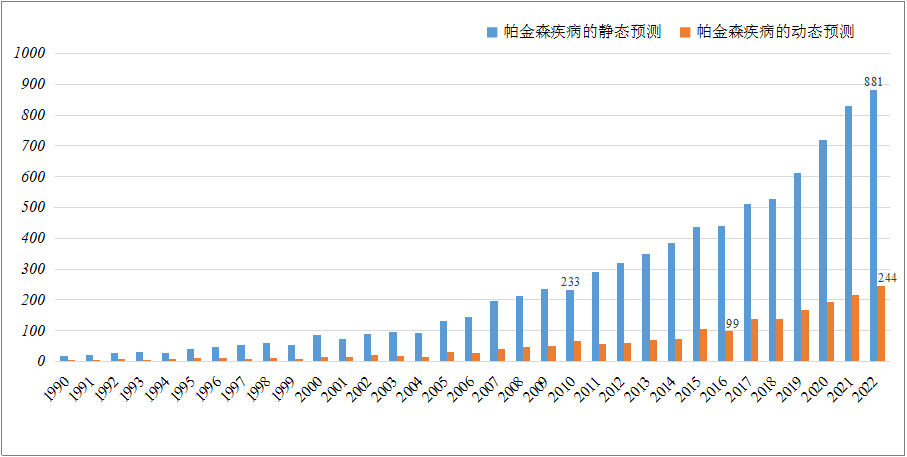
\includegraphics[width=0.9\linewidth]{figs/paper4JinDongTai.png}
      \caption{PD的静态及动态智能辅助预测发文量统计}\label{paper4JinDongTai}
     \end{figure} 

数据的丰富性提高、计算技术的进步以及神经网络设计的优化共同促进了深度学习技术的发展和普及。作为ML领域中的先进技术,深度学习通过构建更加复杂的神经网络来增强模型的表现力和准确度。在PD的预测领域,深度学习方法同样取得了令人瞩目的成效\cite{sivaranjini2020deep,prashanth2016high,vaiciukynas2017detecting,naranjo2016addressing,masud2021crowd,pahuja2022deep,sharanyaa2022optimized,oh2020deep,adams2021improved}。
表\ref{paper4MLpredictJt}和表\ref{paper4MLpredictDt}汇总了近年来运用机器学习技术对帕金森病(PD)进行静态和动态评估的多项研究成果,涵盖了所采用的不同ML技术、数据来源以及预测的准确率(ACC和AUC)。其中,大多数研究倾向于使用传统ML技术,而采用深度学习技术的研究相对少见。数据主要来自PPMI,并且大多数医学影像数据采用的是SPECT。在这些研究中,仅使用单一数据类型进行预测的成功率通常较低,而使用步态周期数据进行预测的成功率较高。同时,将脑脊液(CSF)等临床评分与医学影像数据相结合,能够显著提高预测的性能。


当前,多模态分类预测模型在帕金森病(PD)的研究中正逐渐受到重视并展现出发展潜力。尽管如此,这一领域仍面临诸多挑战,特别是在收集和整合PD患者全面数据方面存在限制。因此,开发无需人工干预即可从多种模态中自动提取特征的早期PD分类预测模型显得尤为重要。这样的模型能够利用更为丰富的数据资源,从而构建更精确的分类预测网络。此外,表\ref{paper4MLpredictDt}的分析表明,目前只有少数研究尝试结合基因数据与医学影像数据来探索它们与PD之间的关联。这种跨模态的数据融合方法有望进一步加深学者对PD遗传背景及其与疾病发展之间联系的理解。


\section{临床信息主导的智能辅助进展预测}\label{chapter5.2:pdCMF-Net}
随着人口老龄化的增加,帕金森病患者也在迅速增加,因此,对评估和跟踪帕金森病进展的动态监测变得越来越重要。为了找到一种更为高效的帕金森病进展预测方法,本节通过分析单模态(DTI、DAT及临床)特征在PD疾病5年后进展预测的临床价值,并提出一种跨模态数据融合(DIT\&临床、DAT\&临床)对帕金森病的进展进行预测的方法(Cross-Modal Fusion prediction model,CMFP)。
该方法的步骤主要是数据准备, 建模, 预测。数据涉及到临床, DTI及DAT这3种模态, 不同模态数据类型均使用Lasso方法进行特征筛选。各单模态采用AdaBoost进行分类, 将结果应用于新的融合策略CMF中得到新的模型。最后使用新的模型进行预测。CMFP在PD进展上的预测获得的AUC为0.7791。与单独的临床数据、DTI数据和DAT数据预测所获得的AUC分别提高了0.2448、0.3078、0.327。测试临床与DTI结合预测相对于单独使用临床数据预测的结果具有统计学显著性, p值为9.183e-4。该方法还确定了与PD相关的关键的脑区和重要的临床指标。本节的研究结果表明, CMFP是有效的, 其有助于改善单模态数据预测性能低的不足, 提高PD进展预测的准确性。并能确定PD的潜在生物标志物信息, 为了解PD提供了新的途径, 值得进一步研究。

\subsection{智能辅助预测的数据与方案}

    \begin{figure*}[ht]
      \centering
      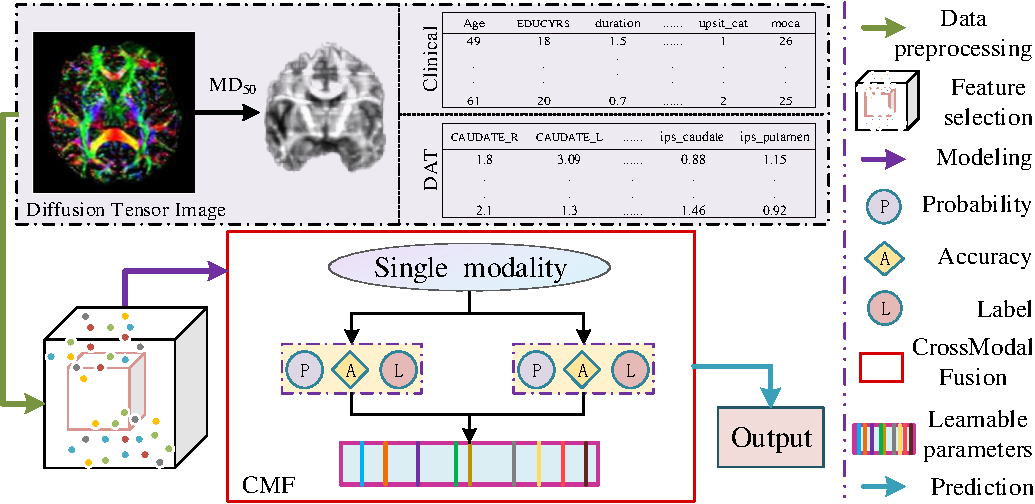
\includegraphics[width=0.9\linewidth]{figs/paper5FrameworkNew.pdf}
      \caption{本节提出的方法(CMFP)框架图}\label{paper5FrameworkNew}
     \end{figure*} 

\subsubsection{进展预测的数据说明}
本项研究利用了帕金森病进展标志物倡议(PPMI)的丰富资源,该资源汇集了多个研究中心的PD患者纵向数据。所有参与PPMI的研究站点均已获得相应伦理审批,且所有参与者在加入前都签署了知情同意书。研究中,本节采用HYS量表会考虑运动功能的退化、生活质量的降低以及多巴胺水平的减少等多个因素,并据此将PD分为五个不同的阶段(1至5期)。研究入选标准包括:至少有5年的纵向随访记录且HYS评分完整的PD患者;基线数据中含有完整的MRI影像资料,包括3D T1WI和DTI扫描;使用3T Siemens MRI进行扫描。筛选条件包括临床信息不完整、成像质量不佳以及图像处理出现失误等情况。

在本研究中,共有123名PD患者符合入选条件。通过分析PPMI数据库中这些患者5年的HYS评分动态,本节观察到74例患者的评分高于初始水平,46例患者评分持平,而3例患者评分低于起始水平。据此,本节将评分提升的患者定义为进展组(共72例),评分未变或下降的患者则归为稳定组(共49例)。研究还收集了一系列临床信息,包括性别、年龄、教育背景以及PD运动评定量表等,并测量了脑脊液中的生物标志物:A$\beta$42、$\alpha-syn$、$t-tau$和$p-tau$的蛋白浓度。123位受试者接受了3T Siemens MRI的非对比增强3D T1加权成像和DTI扫描。DTI影像的预处理使用了PANDA软件,包括去除非脑组织、纠正涡流效应和轻微头部移动、计算DTI矩阵以及应用连续跟踪(FACT)算法进行纤维追踪。若追踪过程中遇到曲率角度大于45°或体素分数各向异性(FA)值小于0.2,则追踪终止。在构ML模型时,本节选取了与PD进展相关的基线期临床指标、DAT水平及DTI脑网络特征作为输入变量,并运用Lasso的方法进行特征选择,旨在提升模型的预测准确度和泛化能力。


\subsubsection{进展预测的特征选择} 
在构建人工智能机器学习模型时,特征选择扮演着至关重要的角色,其重要性不容忽视。不同的特征选择会直接影响模型的预测准确性和在未见数据上的泛化能力。在本节的研究工作中,通过整合基线时的临床参数、多巴胺转运体(DAT)扫描数据以及扩散张量成像(DTI)所揭示的网络特性,本节创建了一个机器学习框架,用以预测五年后PD患者疾病的演变情况。为了提高模型的预测效果,本节对数据进行了严格的预处理,剔除了无效、不规范和错误的数据。
在原始的临床数据中,在本研究中,对16项临床指标进行了系统分析,这些指标包括三类基础信息、九种用于评估运动能力和认知水平的测试量表,以及四项反映脑脊液中蛋白质浓度的生化测量值。通过应用Lasso方法进行特征筛选,本节成功识别并保留了4个最为关键的临床变量(UPDRS Part III Score、UPDRS Total Score、Age、UPSIT score),这些变量与PD的疾病进展有着较高的相关性。对于DTI变量为脑区MD(50)矩阵,也使用Lasso方法进行数据选择,最终选择7个特征(Splenium of Corpus Callosum、Fornix (Column and Body of Fornix)、Inferior Cerebellar Peduncle (Left)、Superior Cerebellar Peduncle (Left)、Fornix (Crescent)/Stria Terminalis (Right)、Tapetum Left、Tapetum Right),分别代表终纹、胼胝体压部、穹窿、左侧小脑下脚、左侧小脑上脚、左内矢状层、右内矢状层这几个脑区。对于DAT数据,也使用Lasso方法进行数据选择,最终选择4个特征:
Putamen Left、High Putamen、Low Striatum和High Striatum,它们分别代表了左侧腹核、高腹核、低纹状体和高纹状体。这样的特征选择策略不仅提高了模型的解释能力,还有助于增强模型预测效果及应对不同情况的广泛适用性。



\subsubsection{跨模态数据融合的进展预测}
本节通过整合基线时的临床参数、多巴胺转运体(DAT)扫描数据以及扩散张量成像(DTI)所揭示的网络特性来训练机器学习模型,用以预测五年后PD患者疾病的演变情况。 在单模态建模过程中, 本节采用AdaBoost算法进行的分类。
AdaBoost(自适应增强算法)是一种集成方法,它能够将多个表现一般的弱分类器协同工作以构建一个强大的综合分类器。其“自适应”体现在:每当一个弱分类器在训练中对某些样本判断错误时,这些样本的权重会被相应增加。随后,在下一轮迭代中,所有样本根据更新后的权重再次参与训练新的弱分类器。此过程不断循环,每轮迭代都会依据全体样本调整权值并确定每个新加入的弱分类器的贡献度,继续迭代直到满足预定错误率条件或达到最大循环次数。AdaBoost能够根据弱分类器提供的信息动态调整错误率预期,并且以高效率运作,已有研究使用AdaBoost对PD进行早期预测\cite{anisha2020early}。

为了进一步改进单变量基线数据对5年后进展预测的性能, 本节采取跨模态数据组合的方式, 并提出一种新的决策策略以提高预测性能。图\ref{paper5FrameworkNew}是本研究的总框架图, 包括数据预处理, 特征筛选, 分类器建模, 预测4部分构成, 具体步骤:
%设置参数、数据准备、单模态训练、多模态融合、循环训练、模型保存、测试集验证
\begin{enumerate}
\item 设置参数epoch=120, 使用Adam作为优化算法, 初始学习率为0.01, 每50个epoch学习率下降0.1, 损失的计算采取的是MSE的计算过程, $\beta$为1 , $\alpha$为0.4;
\item 使用Lasso方法对多模态数据进行特征筛选, 将筛选出的特征作为训练集、验证集和测试集, 并按照6:3:1分配三个子集;%\item 3 分别单独输入两个不同模态的数据的训练集与验证集, 并打乱这两个集合的顺序;
\item 将不同的单模态的训练集数据使用AdaBoost方法进行训练, 得到的模型使用验证集数据进行预测, 得到预测的概率、预测的标签和精确度, 并分别保存单模态训练好的模型;
\item 将不同模态预测的结果(预测的概率、预测的标签和精确度)输入多模态融合算法(CMF:CrossModalFusion)中, 得到一组新的预测结果(预测的概率、预测的标签和精确度), 并保存融合模型;
\item 重复3-5步骤, 直到epoch=120结束循环;
\item 查找单模态训练过程中保存的精确度最高的模型Ms和两模态融合过程中保存的精确度最高的模型Mc。
\item 将测试集数据输入模型Ms, 得到预测的结果(预测的概率、预测的标签和精确度), 并将这组结果输入到模型Mc中进行测试, 得到两模态融合的预测概率和标签。
\end{enumerate}

在决策之前本节获取到了两种单模态数据的预测结果, 包括预测标签, 预测概率及精确度,分别记作$\rho_{a},~\rho_{b},~\eta_{a},~\eta_{b},~\varphi_{1}~and~\varphi_{2}$。根据这些单模态预测结果,使用本节提出的决策策略CMF可以得到决策融合的预测结果$\Phi$,它由预测概率和预测标签组成,即$\Phi = [\rho,~\eta].$。本节定义预测类别的差异$\Omega = abs(\rho_{a} - \rho_{b})$,即两个模型预测的类别之间的绝对差值。准确率的差异的符号$\sigma = sign(\varphi_{1} - \varphi_{2})$,即两个模型准确率之差的符号。sign函数返回-1、0或1,表示差异为负、零或正。预测概率的差异$\upsilon = abs(\eta_{a} - \eta_{b})$,即两个模型预测的概率之间的绝对差值。$\lambda$是通过概率差异$\upsilon$计算的权重。$\mathrm{\lambda=}\iota/(1+\mathrm{e}^{-\alpha * \upsilon} )$。其中,$\iota$为1 ,$\alpha$为0.4; 最终的预测概率和预测标签由公式(\ref{paper5pro})和(\ref{paper5pre})获得,根据$\Omega,~\sigma$和$\upsilon$的取值,选择不同的分支来组合预测结果。 $\zeta(A,~B,~C)$表示条件函数,如果$A$为真,则结果为$B$,否则为$C$。

\if 0
\begin{equation}\label{paper5Ldif}
\mathrm{\lambda=}\iota/(1+\mathrm{e}^{-\alpha * \upsilon} )
\end{equation}
\fi

\if 0
\begin{equation}\label{paper5proB}
\psi=\mathrm{\zeta}(\sigma>0,~\mathrm{\eta_{a}},~\mathrm{\eta_{b}})
\end{equation}

\begin{equation}\label{paper5proC}
\tau=\mathrm{\zeta}(\sigma>0,~\mathrm{\lambda}+\mathrm{\eta_{a}},~\mathrm{\lambda}+\mathrm{\eta_{b}})
\end{equation}

\begin{equation}\label{paper5pro}
\mathrm{\rho}=\mathrm{\zeta}(\Omega=0,~\psi,~\tau)
\end{equation}
\fi


\begin{equation}\label{paper5pro}
\mathrm{\rho}=\mathrm{\zeta}(\Omega=0,~\mathrm{\zeta}(\sigma>0,~\mathrm{\eta_{a}},~\mathrm{\eta_{b}}),~\mathrm{\zeta}(\sigma>0,~\mathrm{\lambda}+\mathrm{\eta_{a}},~\mathrm{\lambda}+\mathrm{\eta_{b}}))
\end{equation}



\if 0
\begin{equation}\label{paper5preB}
\phi=\mathrm{\zeta}(\sigma>0,~\mathrm{\rho_{a}},~\mathrm{\rho_{b}})
\end{equation}

\begin{equation}\label{paper5preC}
\mu=\mathrm{\zeta}(\mathrm{\rho}<0,~-1,~\mathrm{\rho}>0.5,~1,~0)
\end{equation}

\begin{equation}\label{paper5pre}
\mathrm{\eta}=\mathrm{\zeta}(\Omega=0,~\phi,~\mu)
\end{equation}
\fi

\begin{equation}\label{paper5pre}
\mathrm{\eta}=\mathrm{\zeta}(\Omega=0,~\mathrm{\zeta}(\sigma>0,~\mathrm{\rho_{a}},~\mathrm{\rho_{b}}),~\mathrm{\zeta}(\mathrm{\rho}<0,~-1,~\mathrm{\rho}>0.5,~1,~0))
\end{equation}



\subsection{智能辅助预测的实验分析}
本节使用的是Python 3.7.9语言编程,在GNU/Linux x86 64 system of GeForce RTX 3090 Ti 12 Intel Core Interl(R) Xeon(R) CPU E5-2678 v3 2.50GHz 64GB RAM 平台上运行。为了提高模型的性能,在输入模型进行训练与验证之前样本顺序都进行了随机的打乱。

\begin{table}[ht]
\centering
%\scriptsize
\caption{临床数据、DTI数据和DAT数据的特征组合 }
\label{paper5combinations}
%\begin{tabular}{c|ccccccc}
\begin{tabular}{p{1.5cm}<{\centering}|p{1.3cm}<{\centering}p{1.3cm}<{\centering}p{1.3cm}<{\centering}p{1.3cm}<{\centering}p{1.3cm}<{\centering}p{1.3cm}<{\centering}p{1.3cm}<{\centering}p{1.3cm}<{\centering}}
\hline  \hline
\textbf{$\delta_2$} & Age  & UP3s &      &      &           &     &     \\
\textbf{$\delta_3$} & Age  & UP3s & PTs  &      &           &     &     \\
\textbf{$\delta_4$} & Age  & UP3s & PTs  & Uts  &           &     &     \\
\textbf{$\delta_5$} & Age  & UP3s & PTs  & Uts  & STs       &     &     \\ \hline 
\textbf{$\gamma_2$} & SoCC & Fcb  &      &      & \textbf{} &     &     \\
\textbf{$\gamma_3$} & SoCC & Fcb  & ICPl &      & \textbf{} &     &     \\
\textbf{$\gamma_4$} & SoCC & Fcb  & ICPl & SCPl &           &     &     \\
\textbf{$\gamma_5$} & SoCC & Fcb  & ICPl & SCPl & FcSTr     &     &     \\
\textbf{$\gamma_6$} & SoCC & Fcb  & ICPl & SCPl & FcSTr     & TaR &     \\
\textbf{$\gamma_7$} & SoCC & Fcb  & ICPl & SCPl & FcSTr     & TaR & TaL \\ \hline 
\textbf{$\vartheta_2$}    & PuL  & HPu  &      &      &           &     &     \\
\textbf{$\vartheta_3$}    & PuL  & HPu  & LSt  &      &           &     &     \\
\textbf{$\vartheta_4$}    & PuL  & HPu  & LSt  & HSt  &           &     &    \\\hline \hline
\end{tabular}
\end{table}


\subsubsection{不同类型数据预测分析}
使用单一或双模态数据来预测帕金森病(PD)的进展会得到不同的结果。
表\ref{paper5singalAvg_AUC}展示了使用三种模态分别预测PD进展的平均AUC值,可以观察到每个AUC值相对较低。其中,$\Gamma$指的是特征选择,而$\Gamma_i$指代特定的特征组合,$i$表示组合的序号。不同数据集对应不同的特征组合,具体的特征组合显示在表\ref{paper5combinations}中。在表 \ref{paper5combinations}中,$\delta_{i}$,$\gamma_{i}$和$\vartheta_{i}$ 分别代表临床数据、DTI数据和DAT数据的特征组合,其中$i$表示特征组合的数量。$\Gamma_{21}$, $\Gamma_{23}$和$\Gamma_{50}$代表每个模态的所有特征组合。UP3s: UPDRS Part III score,PTs: UPDRS Total Score,Uts: UPSIT score,STs: STAI scores. SCC: Splenium of Corpus Callosum,Fcb: Fornix (Column and Body of Fornix),ICl: Inferior Cerebellar Peduncle (Left),SCl: Superior Cerebellar Peduncle (Left),FcSr: Fornix (Crescent)/Stria Terminalis (Right),TaR: Tapetum Right,TaL: Tapetum Left. PuL: Putamen Left,HPu: High Putamen,LSt: Low Striatum,HSt: High Striatum。


\begin{table*}[ht]
\centering
\caption{单模态数据预测PD进展的平均AUC值}
\label{paper5singalAvg_AUC}
\footnotesize
\begin{tabular}{cccccccccc}
\hline \hline
  & \textbf{$\Gamma_2$} & \textbf{$\Gamma_3$} & \textbf{$\Gamma_4$} & \textbf{$\Gamma_5$} & \textbf{$\Gamma_6$} & \textbf{$\Gamma_7$} & \textbf{$\Gamma_{21}$} & \textbf{$\Gamma_{23}$} & \textbf{$\Gamma_{50}$} \\ \hline
\textbf{Clinical}     & 0.4077      & 0.4371      & 0.4515      & 0.4478      & -           & -           & -            & 0.4629       & -            \\
\textbf{DTI}          & 0.4208      & 0.4476      & 0.4489      & 0.4310      & 0.4770      & 0.4191      & -            & -            & 0.4381       \\
\textbf{DAT}          & 0.5017      & 0.4767      & 0.4631      & -           & -           & -           & 0.4506       & -            & -      \\ \hline    \hline  
\end{tabular}
\end{table*}

   \begin{figure}[ht]
      \centering
      \includegraphics[width=0.85\linewidth]{figs/paper5MAEF1SCOREvariance.pdf}
      \caption{不同策略进行五次预测的MAE和F1 score的方差}\label{paper5MAEF1variance}
     \end{figure}

通过本节提出的跨模态融合预测方法(CMFP),对DTI和DAT的临床组合进行了测试,AUC结果如表\ref{paper5cmfDifferFeature_AUC}所示。其中,$\delta_i$,$\gamma_i$和 $\vartheta_i$分别代表临床数据、DTI数据和DAT数据的特征组合。它们的定义与表 \ref{paper5combinations} 中的相同。 表\ref{paper5cmfDifferFeature_AUC}中的A表示临床数据与DTI的结合预测;B表示临床数据与DAT的结合预测。不同数量的特征选择会导致AUC值的变化,当选择了4个临床特征和7个DTI特征时,结果相对较高,达到了0.7791。因此,在随后的分析中,将以该组合作为实验对象。然而,临床和DAT的联合预测效果相对较差。当选择2个临床特征和DAT特征进行预测时,AUC最高为0.6。使用本节提出的方法,对于预测4个临床特征和7个DTI特征的组合,方差为0.1085。相反,在预测2个临床特征和2个DAT特征的组合八次后,方差为0.1929。总体而言,临床和DTI的联合预测效果优于临床和DAT的联合预测效果。


    \begin{figure*}[ht]
      \centering
      \includegraphics[width=0.95\linewidth]{figs/paper5ROCs_1case.pdf}
      \caption{五种不同策略预测PD进展的ROC曲线对比分析}\label{paper5ROCs_}
     \end{figure*}


在表 \ref{paper5cmfDifferFeature_AUC} 中可以观察到,当将临床数据的 4 个特征与 DTI 数据的 7 个特征结合起来进行预测时,所得到的 AUC 值在所有特征组合中表现最佳。同样地,当将临床数据的 2 个特征与 DAT 数据的 2 个特征结合起来进行预测时,也得到了更优异的 AUC 值。为了更深入地分析单模态数据预测和双模态数据预测的模型性能,计算了MAE和F1分数。图 \ref{paper5MAEF1}(a) 和 (b) 分别展示了五种预测情况的 MAE 和 F1 分数评估结果。其中,Clin-Dti代表临床数据与DTI结合的预测结果,Clin-Dat代表临床数据与DAT结合的预测结果。MAE 用于衡量预测结果与实际观察值之间的平均偏差。较小的 MAE 值表示模型的预测结果更接近真实值。而 F1 分数是基于精确度和召回率的调和平均值,较高的值表示模型的分类性能更好。

\begin{table}[htbp]
\centering
%\footnotesize
\caption{临床数据分别与DTI和DAT融合预测的AUC值}
\label{paper5cmfDifferFeature_AUC}
%\begin{tabular}{|c|ccccc|}
\begin{tabular}{|p{1.1cm}<{\centering}|p{1.8cm}<{\centering}p{1.8cm}<{\centering}p{1.8cm}<{\centering}p{1.8cm}<{\centering}p{1.8cm}<{\centering}|}
\hline
 \textit{\textbf{A}} & $\delta_{23}$         & $\delta_2$                   & $\delta_3$          & $\delta_4$                   & $\delta_5$          \\ \hline 
\textbf{$\gamma_{50}$}               &  0.6409   &  0.4647          &  0.5539  &  0.4873          &  0.4859  \\
\textbf{$\gamma_2$}                &  0.4955   &  0.5113          &  0.5506  &  0.5102          &  0.6459  \\
\textbf{$\gamma_3$}                &  0.5315   &  0.5161          &  0.5053  &  0.5193          &  0.5858  \\
\textbf{$\gamma_4$}                &  0.5458   &  0.4963          &  0.5435  &  0.4566          &  0.6038  \\
\textbf{$\gamma_5$}                &  0.5288   &  0.4936          &  0.4623  &  0.6019          &  0.4905  \\
\textbf{$\gamma_6$}                &  0.4872   &  0.6439          &  0.7096  &  0.5681          &  0.6135  \\
\textbf{$\gamma_7$}                &  0.6677   &  0.5228          &  0.4717  &  \textbf{0.7791} &  0.5172  \\ \hline
 \textit{\textbf{B}}  & $\delta_{23}$         & $\delta_2$                   & $\delta_3$          & $\delta_4$                   & $\delta_5$   \\ \hline 
\textbf{$\vartheta_{21}$}               &  0.5759   &  0.4670          &  0.4144  &  0.4606          &  0.4960  \\
\textbf{$\vartheta_2$}                &  0.5592   &  \textbf{0.6000} &  0.5683  &  0.5694          &  0.5842  \\
\textbf{$\vartheta_3$}                &  0.5591   &  0.5990          &  0.4982  &  0.4657          &  0.5146  \\
\textbf{$\vartheta_4$}                &  0.5729   &  0.5207          &  0.5518  &  0.5130          &  0.5882      \\
\hline 
\end{tabular}
\end{table}

   \begin{figure}[ht]
      \centering
      \includegraphics[width=0.95\linewidth]{figs/paper5MAEF1SCORE.pdf}
      \caption{采用不同策略进行五次预测PD进展的MAE和F1得分的平均值}\label{paper5MAEF1}
     \end{figure}

在图 \ref{paper5MAEF1}(a) 的展示中,可以发现在三种单模态数据预测方法中,基于DTI数据的预测方法在平均绝对误差(MAE)方面取得了最优表现。而在两种双模态数据融合预测中,结合临床数据与DTI数据的预测方法在MAE上展现出了更佳的性能。进一步地,图 \ref{paper5MAEF1}(b) 揭示了五种预测方法中,临床数据和DTI数据结合的预测方法在F1得分上位居首位。此外,单模态预测的F1得分显著低于双模态预测的F1得分。另外,对不同预测方法在MAE和F1得分上的方差进行计算,结果如图 \ref{paper5MAEF1variance} 所示。

\if 0
    \begin{figure*}[h]
      \centering
      \includegraphics[width=0.7\linewidth]{figs/paper5accemsemae.pdf}
      \caption{采用不同ML技术的模型性能对比}\label{paper5accemsemae}
     \end{figure*}
\fi
     
    \begin{figure*}[ht]
      \centering
      \includegraphics[width=0.85\linewidth]{figs/paper5accML.pdf}
      \caption{嵌入不同ML技术的模型ACC对比分析}\label{paper5accML}
     \end{figure*}

     
    \begin{figure*}[ht]
      \centering
      \includegraphics[width=0.85\linewidth]{figs/paper5rmsemaeML.pdf}
      \caption{嵌入不同ML技术的模型RMSE与MAE对比分析}\label{paper5rmsemaeML}
     \end{figure*}
     
\subsubsection{集成机器学习技术分析}
在本研究中,提出了一个集成了Adaboost算法的新模型。为了验证该模型的有效性,对其进行了一系列的性能测试,并将结果与其他几种流行的ML技术(支持向量机(SVM)、逻辑回归(LR)、高斯朴素贝叶斯(GaussianNB)、K最近邻(KNN)、决策树(DT)、随机森林(RF)、极端树(ExtraTree))进行了对比,如图~\ref{paper5accML}和图~\ref{paper5rmsemaeML}所示。本节采用了准确率(ACC)、均方根误差(RMSE)和平均绝对误差(MAE)这三个核心指标来衡量模型的预测能力。
ACC是衡量分类模型性能的常用标准,它反映了模型正确预测的样本占总样本数的比例。当准确率接近1时,表明模型具有极高的预测准确性。
RMSE则提供了预测值与实际值之间差异的量化度量。由于它是误差的平方根,因此对于较大的误差值,RMSE会更加敏感。一个较低的RMSE值意味着预测模型在数据拟合上更为精准。
MAE同样衡量预测值与实际值之间的差距,但与RMSE不同的是,MAE对所有误差值赋予相同的权重,因此它对异常值的影响较小。一个较低的MAE值通常指示着模型的预测误差较小,即模型性能较好。

\if 0
    \begin{figure*}[h]
      \centering
      \includegraphics[width=0.7\linewidth]{figs/paper5aucroc.pdf}
      \caption{通过采用其他ML算法替代Adaboost的四项评价指标比较分析}\label{paper5aucroc}
     \end{figure*}
\fi
     
    \begin{figure*}[ht]
      \centering
      \includegraphics[width=0.85\linewidth]{figs/paper5aucML.pdf}
      \caption{嵌入不同ML技术的模型AUC对比分析}\label{paper5aucML}
     \end{figure*}
     
    \begin{figure*}[ht]
      \centering
      \includegraphics[width=0.95\linewidth]{figs/paper5rocML.pdf}
      \caption{嵌入不同ML技术的模型ROC对比分析}\label{paper5rocML}
     \end{figure*}

通过图~\ref{paper5accML}到图~\ref{paper5rocML}的直观展示,本节的方法在所有三个性能指标上都表现出色。特别是在ACC方面,本节的模型比其他算法表现得更为突出,比排名第二的随机森林算法(RF)高出了6.73个百分点。在RMSE和MAE的数值对比上,本节的模型也显示出了相对于RF算法分别低6.81\%和6.73\%的显著优势。
综上所述,本节的模型不仅在理论上设计精巧,而且在实际应用中也展现出了卓越的预测性能。这些结果充分证明了本节提出的方法在处理相关问题时的有效性和优越性。

\subsection{进展预测模型的探索与发现}  
弥散张量成像(DTI)作为一项先进的磁共振成像技术,已在近年来得到迅速发展。它利用多个不同强度的扩散敏感梯度,能够精确地描绘出人体内水分子的扩散能力及其移动方向,从而深入揭示生物组织,尤其是脑组织的微观结构特点。这种成像技术不需要对活体进行任何侵入性操作,便能直观地观察和分析白质纤维束的完整性和方向性,这对于研究神经系统的疾病具有重要意义。一些学者基于弥散张量成像(DTI)的研究探索了白质的变化,并发现与对照组相比,PD-MCI患者的额叶白质损伤更为显著,且与整体认知功能的损害以及多个认知领域的损害存在关联\cite{wang2020changes}。对于PD的复杂多样的神经机制,通过整合多种模态MRI特征,从多个层面和不同角度进行综合评估和分析,为进一步提高PD早期诊断和干预提供了潜在的生物标志物\cite{pyatigorskaya2018comparative,gu2016automatic,bowman2016multimodal}。Pyatigorskaya等人\cite{pyatigorskaya2018comparative}研究者结合了NMS-MRI中的黑质体积和信号强度特征以及DTI中的部分各向异性特征,成功地将PD诊断的准确率提升至93\%。Lei等人\cite{lei2018longitudinal,lei2017joint}开发的基于MRI和DTI的预测模型能够智能识别PD,并对临床评分进行准确预测,这在临床实践中具有重要的应用价值。Chougar等人\cite{chougar2021automated}则进一步探索了如何利用脑区(13个大脑区域)体积和DTI参数作为输入,并使用监督ML算法准确预测PD、PSP和MSA-P的分类。Shin等人\cite{shin2021cortical}的研究关注了MRI皮层厚度在预测PD患者从轻度认知障碍向痴呆转变中的作用。他们的研究结果显示,MRI皮层厚度能够有效预测个体的疾病进展,并且当与临床数据相结合时,其预测性能得到了进一步提升。这一发现强调了MRI技术在个体化医疗和精准治疗策略制定中的重要作用。

通过合并表 \ref{paper5singalAvg_AUC} 和表 \ref{paper5cmfDifferFeature_AUC} 中的数据,可以确定对PD预测贡献相对显著的临床指标,进而推断出与PD进展相关的潜在特征。这些关键的临床数据特征包括年龄、UPDRS第三部分分数、UPDRS总分以及UPSIT分数。

当前,可靠的网络表征技术的发展为在全脑连接层面理解神经疾病提供了新的途径。然而,目前关于使用白质数据来预测帕金森病(PD)进展的研究相对有限。Wee等人\cite{wee2011enriched}开发了一种基于网络的多变量分类算法,该算法利用白质纤维束数据,能够有效区分正常对照组和轻度认知障碍(MCI)患者。研究结果显示,这种分类框架能够为临床诊断以及与认知障碍相关的脑结构变化提供一种创新的替代和辅助手段。尽管如此,这项研究主要集中在阿尔茨海默病领域,对于PD的应用尚需进一步探索。


在本研究的预测模型中,除了纳入临床特征,还挑选了七个来自DTI变量的特征,这些特征涉及到脑白质的MD。研究发现,这些脑白质的特征在预测PD的发展进程方面具有重要作用,并且当与传统的临床特征相结合时,能够显著提升模型的预测准确性。
具体来说,仅依赖DTI全球白质特征构建的预测模型获得了0.44035的AUC值(方差为0.0185),而独立使用临床特征的模型AUC值稍高,为0.4414(方差为0.0187)。然而,当这两类特征被整合到同一个预测模型中时,模型的性能得到了显著的增强,AUC值跃升至0.7791(方差为0.1085),这表明DTI白质特征与临床特征之间存在着互补作用,共同为预测PD提供了更加丰富和精确的信息。


多模态融合技术通过整合来自不同来源和类型的数据,能够提供更为丰富和立体的信息,从而在理解复杂的生物医学问题时发挥着至关重要的作用。在PD的研究中,多模态融合尤其展现了其独特优势。例如,结合临床症状评估、扩散张量成像(Diffusion Tensor Imaging, DTI)和多巴胺转运体(Dopamine Transporter, DAT)显像等多种数据源,不仅能够揭示PD患者大脑结构和功能的细微变化,还能帮助医生更准确地评估病情的严重程度和进展速度。
图\ref{paper5ROCs_}所展示的五条ROC曲线直观地证明了多模态融合的有效性。在图\ref{paper5ROCs_}中,不同的颜色用于表示不同数据组合的预测结果。特别是在图(b)中,阴影区域展示了置信区间。分析结果指出,将临床数据与DTI或DAT影像数据结合使用的多模态方法,相较于单一数据源的预测方法,在预测帕金森病进展方面更为精确。尤其是将临床数据与DTI数据相结合的方法,展现出了最优的预测效果。单独使用某一种数据源的曲线(如临床数据、DTI数据或DAT数据)通常只能提供有限的信息,而一旦将这些数据结合起来,ROC曲线就会明显上升,表明模型的预测能力得到了显著提升。特别是当临床数据与DTI数据结合时,预测性能的提升尤为显著,这进一步验证了多模态融合在提高PD预测准确性方面的潜力。

\begin{table}[ht]
\centering
\caption{临床数据分别与DTI和DAT相结合进行预测}
\label{paper5twoClinDtiDat}
%\small
%\begin{tabular}{ccccc}
\begin{tabular}{p{2.3cm}<{\centering}p{2.2cm}<{\centering}p{2.2cm}<{\centering}p{2.2cm}<{\centering}p{2.2cm}<{\centering}}
\hline
\textit{Avg} & \textbf{AUC} & \textbf{ACC} & \textbf{SEN} & \textbf{SPE} \\ \hline
Clin-Dti           & \textbf{0.7791}       & \textbf{0.8077}       & \textbf{0.9464}       & \textbf{0.7470}       \\
Clin-Dat           & 0.6000       & 0.7385       & 0.8679       & 0.6298     \\ \hline
\textit{Vac} & \textbf{AUC} & \textbf{ACC} & \textbf{SEN} & \textbf{SPE} \\ \hline
Clin-Dti             &\textbf{0.1085}   & 0.1490       & 0.1417       & 0.1890       \\
Clin-Dat           & 0.1929    & \textbf{0.0923}      & \textbf{0.1041}       & \textbf{0.1516}     \\ \hline
\end{tabular}
\end{table}

正如表\ref{paper5singalAvg_AUC}、表\ref{paper5cmfDifferFeature_AUC}以及图\ref{paper5ROCs_}所展示的,将临床数据与DTI数据结合起来进行预测,其效果优于结合临床数据与DAT数据。此外,本节还进行了Mann-Whitney U检验,该检验进一步证实了临床数据与DTI数据结合预测的显著性,其结果在统计学上显著优于单独使用临床数据,p值达到了9.183e-4。这一结果强调了多模态数据融合在提高预测准确性方面的潜力。


  \begin{figure}[ht]
      \centering
      \includegraphics[width=0.85\linewidth]{figs/paper5F1_MLs2.pdf}
      \caption{嵌入不同ML技术的模型F1 score对比分析 }\label{paper5F1_MLs}
     \end{figure}

为了深入比较临床数据与DTI及DAT数据结合的预测效果,采用了ACC(准确率)、SEN(灵敏度)和SPE(特异性)这三项关键指标进行了详尽的分析,并将结果呈现于表\ref{paper5twoClinDtiDat}中。该表格所展示的数据是在经过8次测试后,各项指标的平均值(Avg)和方差值(Vac)。通过观察可以清晰地发现,在将临床数据与DTI数据相结合的情况下,无论是哪一项指标,其表现均显著优于其他组合,这一结果凸显了多模态融合在提高预测准确性方面的重要价值。

为了展现本节方法的卓越性,对不同机器学习算法替代情境下的AUC值进行了详细分析。AUC作为衡量模型分类能力的指标,其值从0至1不等,数值越大表明模型的性能越优。图\ref{paper5aucML}和图\ref{paper5rocML}可见,即使在AUC值上SVM算法排名第二,本节的方法仍领先SVM 2.09个百分点。

本节还计算了各模型的F1分数,并将结果呈现于图\ref{paper5F1_MLs}。从图中可以明显看出,本节的方法在F1分数上取得了最佳成绩,相比RF高出了7.19\%。虽然SVM在AUC指标上位居第二,但在F1分数方面却表现不佳。根据多维度的评估结果,本节的方法展现出了卓越的性能,证实了其在实际应用中的可靠性和稳定性。

综上所述,本节的研究发现将DTI的白质纤维束数据与临床特征相结合,能够显著提高对PD进展的预测能力。通过采用本文提出的CFMP方法构建的网络模型,不仅能够有效评估PD患者的疾病严重度,还能实时监控疾病的进展情况。这一突破性成果对于改进PD的早期诊断和治疗方案具有深远的影响,有望为患者提供更加精准和个性化的医疗服务,从而改善他们的生活质量。

\subsubsection{小结}
PD的发展是一个缓慢而持续的过程,其确诊通常依赖于临床表现和体征。随着疾病进入中期至晚期,治疗变得复杂且困难。因此,早期预测疾病进展对于实施及时有效的干预方案极为关键。但是,迄今为止还未发现精准的生物指标可以预判PD的病程发展,因此,构建一个能早期智能诊断该疾病的模型对于临床实践具有重大的意义。
DTI是一种能够量化大脑内水分子扩散性能的技术,它能够准确地衡量大脑中白质束的结构完好性,并且有助于识别早期病症的潜在迹象。本小节的研究采用基于纵向数据的研究方法,结合ML技术,整合早期PD患者的DTI数据和临床特征,构建了一个疾病进展预测模型。该模型有望为PD的早期诊断和治疗决策提供有力的影像组学支持。
该小节主要局限性在于仅利用了脑白质的平均扩散率(MD)指标进行分析,未能纳入其他相关指标,如分数各向异性(FA)和纤维密度(FN)等。此外,研究未从其他数据库获取数据来验证模型的泛化能力。在未来的研究中,将探索多模态融合分析,包括脑灰质结构数据、基因信息等,以期对PD及其他神经退行性疾病进行更深入的理解和研究。




\section{本章小结}
本章节主要对PD的预测展开了研究与分析,包括PD的静态与动态预测。其中,
在第\ref{chapter5.1:pdPredictReview}节中,回顾了基于ML的智能辅助帕金森疾病分类预测,强调ML技术的发展为帕金森病的智能诊断与健康测评提供了解决误诊或无法确诊的解决方案。通过对分类器训练的概述,强调了ML模型在挖掘大量数据中潜在规律方面的关键作用。
在第\ref{chapter5.2:pdCMF-Net}节中,提出了一种CMFP方法,基于跨模态数据融合的ML,用于智能辅助PD进展预测。该方法结合了DTI和临床特征数据,强调了PD疾病进展的漫长过程和对早期预测的需求。研究发现跨模态结合预测提高了单模态预测的准确性,DTI数据对临床预测性能的提升具有显著作用。
然而,本节的研究未涵盖神经科学机制,未来需要更深入地结合方法与神经科学,以提高准确性。
% !TEX root = ../main.tex
\chapter{总结与展望} \label{chapter:Conclusions}
人工智能的飞速进步为人类探索生命奥秘开辟了广阔天地,尤其在处理生老病死等根本问题时,人们对健康和长寿的追求从未停止。在医疗领域,人工智能的广泛应用正引领着一场深刻的变革:它不仅在临床诊断中协助医生和放射科专家提高工作效率、降低误诊概率,同时让患者得以获取更多的医学信息,增强了对自身病情的理解,显著提升了他们的健康意识。

影像组学的兴起为医疗影像分析带来了前所未有的革新,它为医生提供了全新的诊断工具。通过整合不同模态的影像数据与关键的临床信息,如基因数据和病理信息,影像组学能够为医生呈现更全面、更精确的疾病影像。
深度学习在影像组学中的运用为整合这些数据提供了强大的支持。深度学习模型能够自动学习并挖掘多模态数据间的复杂联系,发现隐藏在数据背后的模式与规律。借助深度学习技术,影像组学能够更精确地定位和分析疾病特征,为医生提供更为可靠的辅助诊断信息。这种高度智能化的方法不仅提高了诊断的准确度,还加速了医学界对疾病机理和治疗方法的深入理解。

本研究专注于基于医学影像组学的辅助诊断算法以及其在临床实践中的应用。通过紧密结合临床需求,运用融合多模态数据及深度学习技术的手段,成功实现了对脑肿瘤、阿尔茨海默病(AD)和帕金森病(PD)的智能辅助诊断。在临床医生的指导和支持下,本文完成了以下研究工作:
\begin{enumerate}
\item 提出两种多模态融合的方法,成功在两模态的医学影像数据融合方面取得显著效果。这为更全面、多角度地理解患者病情提供了可行性,并且在提高诊断准确性方面具有重要意义;
\item 引入一种新的网络模型,该模型在对AD进行细粒度多分类任务中表现出较高的精度。这一模型的应用不仅提高了诊断的准确性,同时也为更细致的疾病分类奠定了坚实的基础;
\item 深入调研并综述了帕金森病分类预测的研究现状及趋势,并针对跨模态数据融合提出了一种创新的PD进展预测模型。这种模型有望为未来更加精准的帕金森病预测提供新的思路和方法。
\end{enumerate}


当前研究尚处于初级阶段,未来有望探索以下几个研究方向:

(1)全面整合临床数据: 未来的研究将更加强调对临床数据的全面整合,特别是将基因数据与影像数据相结合用于辅助诊断。在影像组学的理念下,将医学数据看作一个复杂的网络,通过将来自不同来源的数据相互关联,协同构建患者的整体健康画像。这种多模态数据的整合,尤其是与基因数据和病理信息的结合,将为医生提供更全面的疾病理解,为个性化治疗方案的制定提供更准确的依据,从而提高治疗的针对性和有效性。

(2)网络模型的优化与设计: 将进一步优化网络模型,设计更适应医疗诊断需求的结构。考虑采用更先进的策略,例如卷积神经网络(CNN)与图卷积网络(GCN)的结合,以提高模型性能。通过深入研究和改进网络结构,期望能实现更准确、可靠且高效的医学影像辅助诊断模型。这将有助于提高诊断的准确性,使其更适应不同疾病特征的处理,并更好地满足临床医生的实际需求。

(3)神经科学与深度学习的融合: 未来的研究将致力于将神经科学的原理与深度学习应用相融合,以更深层次地探索潜在的疾病与感兴趣区域(ROI)之间的关系,从而进一步提高预测精度。通过深入研究大脑神经网络的结构和功能,可以更好地理解不同疾病对特定脑区域的影响。深度学习模型在此过程中将学习并捕捉微妙的神经影像特征,有望揭示潜在的疾病标志物。

(4)强化医疗AI安全框架:鉴于医疗数据敏感性,未来的医学影像系统需内置强大的安全措施,如专用加密确保数据安全,区块链技术保护隐私与数据完整性,及动态监控防御网络攻击。通过融合深度学习与先进网络安全技术,构建智能安全的医疗数据生态,推动精准医疗同时,维护数字医疗环境的安全信任,保障医患利益。

这些研究方向将为医学影像组学辅助诊断领域提供新的动力和方向,有助于更好地迎接临床挑战,为患者提供更为个性化、精准的医疗服务。
\appendix  % 附录

\backmatter  %% 附件部分
\bibliographystyle{style/gbt7714-2005-numerical}

% 参考文献使用 BibTeX
\bibliography{reference/myref}

% \nocite{*} %如果需要列出所有参考文献, 即使这些参考文献没有被正文引用到

\ifblind
\else
  % !TEX root = ../main.tex
\chapter{简称列表}
  
\begin{longtable}{p{2.5cm}<{\centering}p{10.0cm}<{\centering}}
%\caption{中英文的简称列表}\centering
  \hline
  \textbf{英文简称} & \textbf{中文含义及英文全称}  \\  \hline
  \endfirsthead % 表示这是第一页的表头
  \hline
  \textbf{英文简称} & \textbf{中文含义及英文全称} \\ % 后续页表头,与第一页相同
  \hline
  \endhead
  % 表格内容部分
%\hline
%简称 &全称     \\ \hline
AI & 人工智能(Artificial intelligence)   \\ 
DL & 深度学习(Deep Learning) \\ 
AD    &阿尔茨海默症(Alzheimer's disease)    \\ 
PD    & 帕金森疾病(Parkinson's disease)  \\
CT  & 计算机断层成像(Computed Tomography)    \\
MRI    &磁共振成像(magneticrResonance imaging)    \\ 
SPECT  & 单光子发射计算机断层显像(single-photon emission computed tomograph)    \\
PET  & 正电子发射型计算机断层显像(Positron Emission Tomography)    \\ 
fMRI  & 功能性磁共振成像(functional magnetic resonance imaging)    \\
sMRI  &结构磁共振成像(structural Magnetic Resonance Imaging)    \\
X-Ray  &X射线(X Radiography) \\
Microscopy    &显微影像(Microscopic Imaging)    \\
 US   &超声成像(Ultrasound)    \\
DTI  &弥散张量(Diffusion Tensor Imaging)     \\
DAT  &多巴胺转运蛋白(Dopamine transporter)     \\
NC  & 正常认知(Normal Cognition)    \\
EMCI  & 早期轻度认知障碍(Early Mild Cognitive Impairment)    \\
LMCI  & 晚期轻度认知障碍(Late Mild Cognitive Impairment)    \\
SOTA  &最前沿的技术水平(state-of-the-art)     \\
 NSCT   &非子采样轮廓波变换(Non-Subsampled Contourlet Transform)    \\
 CNN   &  卷积神经网络(Convolutional Neural Network)  \\
 GAN   & 生成对抗网络(Generative Adversarial Network )   \\
DDcGAN    &带有双重鉴别器的条件式生成对抗网络(Dual-Discriminator Conditional Generative Adversarial Network)    \\
 ROI   & 感兴趣区域(Region of Interest)   \\
 SVM   &支持向量机(support vector machine)    \\
DBM    &玻尔兹曼机(Deep Boltzmann Machine)    \\
GLCM    & 灰度共生矩阵(Gray-Level Co-occurrence Matrix)   \\
SCD    & 主观认知下降(Subjective Cognitive Decline)   \\
 VBM   &基于体素的形态测量学(voxel-based morphometry)    \\
PCA    &主成分分析(Principal Component Analysis)  \\
rs-fMRI    & 静息态功能磁共振成像(Resting-state functional magnetic resonance imaging)   \\
 PDD   &PD患者常伴有帕金森病痴呆(Parkinson’s disease dementia)    \\
 MoCA   & 蒙特利尔认知评估(Montreal Cognitive Assessment)  \\
 DRS-2   & 马蒂斯痴呆分级量表(Mattis Dementia Rating Scale, 2nd Edition)   \\
 MMSE   &简易的精神状态测评表(Mini-Mental State Examination)    \\
 SOM   & 自组织映射(Self-Organizing Map)   \\
  RMSE   & 均方根误差(Root Mean Square Error)    \\
 R2    &决定系数(Coefficient of Determination)     \\
MAE     & 平均绝对误差(Mean Absolute Error)    \\
 MSE    & 均方误差(Mean Squared Error)    \\
  RMSE   & 均方根误差(Root Mean Squared Error)    \\
MAPE    &平均绝对百分比误差(Mean Absolute Percentage Error)  \\
  EN   &信息熵(Entropy)     \\
  MI   & 互信息(Mutual Information)    \\
FMI  &特征互信息(Feature Mutual Information)   \\
$Q_E$   &边缘相关融合质量(Edge Correlation Fusion Quality)  \\
AG   &平均梯度(Average Gradient)  \\
 SSIM    & 结构相似性(Structural Similarity Index)    \\
  SD   & 标准差(Standard Deviation)    \\
SF   & 空间频率(Spatial Frequency)    \\
rSFe  & 空间频率误差比(the ratio of spatial frequency error )     \\
VIF    & 视觉信息保真度(Visual Information Fidelity)    \\
CC   &相关系数(Correlation Coefficient)   \\
ACC    &准确率(Accuracy)     \\
ROC    & 受试者工作特征曲线(Receiver Operating Characteristic)    \\
AUC  & 曲线下面积(Area Under the Curve)    \\
SEN     &敏感性(Sensitivity)   \\
SPE   & 特异性(Specificity)   \\
TP     & 真正例(True Positive)    \\
TN     & 真负例(True Negative)    \\
FP     & 假正例(False Positive)    \\
 FN    & 假负例(False Negative)    \\
MS-Info & 医学语义信息(medical semantic information)     \\
WCU  & 小波卷积单元(Wavelet Convolution Unit)     \\
WM  & 白质(White matter)     \\
BN  & 批归一化(Batch Normalization)    \\
FA  &分数各向异性(Fractional Anisotropy)      \\
MD  & 平均扩散系数 (Mean Diffusivity)    \\
CSF  & 脑脊髓液(Cerebro spinal fluid)     \\
RNA  & 核糖核酸(ribonucleic acid)     \\
REM  &眼皮快速颤动(arapid eye movement)      \\
UCI  & University of CaliforniaIrvine     \\
PPMI  & The Parkinson’s Progression Markers Initiative     \\
GMM  & 高斯混合模型(Gaussian mixture models)     \\
OPF  & 优化路径森林(optimum-path forest)     \\
DNN  & 深度神经网络(deep neural network)     \\
NB  &贝叶斯(Naive Bayes)      \\
GaussianNB  & 高斯朴素贝叶斯(Gaussian Naive Bayes)    \\
MLP    &多层感知机(multi-layer perceptron)    \\
KNN    &K近邻算法(K-nearest neighbour)    \\
LR    & 逻辑回归(logistic regression)   \\
 GBT   &  梯度提升(gradient boosting tree)  \\
DBN  &  深度信念网络(Deep Belief Network)  \\
  SVR  &  支持向量回归(support vector regression) \\
 RF   &随机森林(random forest)    \\
 DT   & 决策树(decision tree)   \\
ExtraTree  & 极端随机树(extremely randomized trees)    \\
XGBT  &  极端梯度提升(eXtreme gradient boosting tree)   \\
CROWD  & 乌鸦搜索和深度学习组合分类模型(crow search and deep learning)     \\
CERNNE  & 聚类进化随机集成神经网络(clustering evolutionary random neural network ensemble)  \\
vGRFs  & 垂直地面反作用力(vertical ground reaction forces)     \\
CDTW  & 连续动态时间归整(continuous dynamic time warping)     \\
\hline
%\end{tabular}
\end{longtable}
%\end{table}  % 简称列表
  % !TEX root = ../main.tex
\begin{publications}{99}
\ifphd
\addcontentsline{toe}{chapter}{\bf Papers published in the period of doctor education}
\else
\addcontentsline{toe}{chapter}{\bf Papers published in the period of master education}
\fi
%\thispagestyle{empty}

%%盲审时候提交版本
\if 0
\item[1.]
**. ------------ [J]. \textit{IEEE Transactions on Multimedia (TMM)}.  (第一作者, Q1, 中科院一区, 影响因子:7.3,已发表)

\item[2.]
**. ------------ [J]. \textit{IEEE Transactions on Biomedical Engineering (T-BME)}.  (第一作者, Q1,中科院二区, 影响因子:4.6,已发表)

\item[3.]
**. ------------ [J]. \textit{IEEE Transactions on Image Processing (TIP)} (第一作者, Q1, 中科院一区, 影响因子:10.6,已录用)

\item[4.]
**. ------------ [J].\textit{npj Parkinsons Disease}. (第一作者, Q1, 中科院一区, 影响因子:8.7,审稿中)

\item[5.]
**. ------------ [J].\textit{图学学报}. (第一作者, 中文核心,已发表)

\item[6.]
**. ------------ [C]. \textit{ML4CS}.  (共一作者, EI会议, EI检索,已发表)


\item[7.]
**. ------------ [J]. \textit{放射学实践}. (第二作者,中文核心, 已发表)

\fi



%%正式答辩后提交版本
%\if 0
\item[1.]
\textbf{Jinyu Wen}, Asad Khan, Amei Chen, Weilong Peng, Meie Fang, Ping Li and C. L. Philip Chen. High-Quality Fusion and Visualization for MR-PET Brain Tumor Images via Multi-Dimensional Features[J]. \textit{IEEE Transactions on Image Processing}, May 2024, published online, DOI: 10.1109/TIP.2024.3404660. (中科院一区,IF:10.6)

\item[2.]
\textbf{Jinyu Wen}, Feiwei Qin, Jiao Du, Meie Fang, Ping Li, Xinhua Wei, and C. L. Philip Chen. MsgFusion: Medical Semantic Guided Two-Branch Network for Multi-Modal Brain Image Fusion[J]. \textit{IEEE Transactions on Multimedia}, 26, 944-957, 2024.  (中科院一区,IF:7.3)

\item[3.]
\textbf{Jinyu Wen}, Yang Li, Meie Fang, Lei Zhu, David Dagan Feng, and Ping Li. Fine-Grained and Multiple Classification for Alzheimer's Disease with Wavelet Convolution Unit Network[J]. \textit{IEEE Transactions on Biomedical Engineering}, 70(9), 2592-2603, 2023.  (中科院二区,IF:4.6)

\item[4.]
\textbf{Jinyu Wen}, Amei Chen, Meie Fang, Xinhua Wei. Computer aided prediction of Parkinson's disease progression by machine learning from cross-modal data[J]. \textit{npj Parkinsons Disease}. (审稿中,中科院一区,IF:8.7)

\item[5.]
\textbf{温金玉}, 方美娥. 基于机器学习的计算机辅助帕金森疾病分类预测研究综述[J].\textit{图学学报}, 44(6), 2023. (中文核心)

\item[6.]
Danyang Yao, \textbf{Jinyu Wen}, Amei Chen, Meie Fang, Xinhua Wei, Zhigeng Pan. Trimodal Fusion Network Combined Global-Local Feature Extraction Strategy and Spatial-Frequency Fusion Strategy. \textit{ML4CS} (3): 212-226, 2022.  (共一,EI会议收录)

\item[7.]
陈阿梅, \textbf{温金玉}, 黄俊祥, 成小芳, 阮秀杭, 方美娥, 魏新华. 血管周围间隙扩散张量成像指数在评估帕金森病患者脑类淋巴系统功能中的价值[J]. \textit{放射学实践}, 8: 954-959, 2022. (中文核心)

\item[8.]
Jipeng Hu, \textbf{Jinyu Wen}, Meie Fang. A survey on adversarial attack and defense of deep learning models for medical image recognition[J]. \textit{Metaverse} 2023; 4(1): 17,2023. 

\item[9.]
Asad Khan, Sakander Hayat, Muhammad Ahmad, \textbf{Jinyu Wen}, Muhammad Umar Farooq, Meie Fang, Wenchao Jiang. (2022). Cross‐modal retrieval based on deep regularized hashing constraints[J]. \textit{International Journal of Intelligent Systems}, 37(9), 6508-6530. (中科院 二区,IF:7)


\item[10.]
方美娥, 姚丹阳, \textbf{温金玉}. 一种基于深度学习的多模态医学图像融合方法. 2022-08-05, ZL 202210936228.6
%\fi




\end{publications}
     % 发表文章目录
  % !TEX root = ../main.tex
\begin{projects}{99}
\ifphd
\addcontentsline{toe}{chapter}{\bf Projects Participated in the period of doctor education}
\else
\addcontentsline{toe}{chapter}{\bf Projects Participated in the period of master education}
\fi
%\thispagestyle{empty}

\item[1.]
%主持****研究生“基础创新”项目《 ------------ 》(项目编号: ****** )
主持广州大学研究生“基础创新”项目《基于张量计算的多模态医学图像脑网络构建及AD/MCI细粒度分类诊断应用研究》(项目编号:2021GDJC-D16)

\item[2.]
%参与国家自然科学基金项目《 ------------ 》(项目号: ****** )
参与国家自然科学基金项目《CAGD 与 CAD/CAE/AI 深度融合的类B样条等几何方法研究》(项目号:62072126 )

\item[3.]
%参与**市重点研究计划项目《 ------------ 》(项目号: ****** )
参与广州市重点研究计划项目《基于类B样条的等几何边界元分析及形状优化》(项目号:202102010439)

\end{projects}
 % 参与项目目录
  % !TEX root = ../main.tex
\begin{thanks}
\addcontentsline{toe}{chapter}{\bf Acknowledgement}
%\thispagestyle{empty}

白驹过隙,时光匆匆。行文至此, 多年的学生时代即将谢幕,回首过去,仿佛一场梦。四年的博士生活在紧张而充实的科研中默默度过,回顾这段难忘的时光,心头留下了痛苦的泪水,也回荡着欢乐的笑声,然而更多的是对经历困难后那抹明媚阳光的深刻感受。

我清晰地记得,在开始写作的第一周里,每天都凝望着论文题目下的一片空白,愁眉不展,默许着心底涌动的渴望。随着日子一天天流逝,当我在反复修改论文框架时,心急如焚,突然想起年幼时母亲对我说的一句普通却蕴含哲理的话语。
我出生于群山环抱的乡村,在高中之前时常与黄土为伍。小时候,我喜欢和小伙伴在家乡的田野间玩家家,用泥土捏出各种形状的食物,搭建简陋的灶台,甚至用泥巴堆起小墙,划定自己的领地。到了不再玩家家的年纪,每天放学后都帮助家人从事各种农活。其中最难忘的是在炎热的夏天下地处理烟杆。或许很多人对烟杆不了解,也不清楚它的意义。我的老家位于闽西北地区,大多数家庭都务农,上半年种烟叶,下半年转种水稻。没错,烟叶就是那个“吸烟有害健康”包装盒里的原材料,但它让我们的村实现了小康。种烟叶不仅能够维持生计,还能积攒一些存款。每年暑假烟叶都已基本采收结束,每到这个时候,就逃不过处理剩余烟杆,将田地改成水田以便种植水稻。回忆那时,望着一片又一片的烟田,心头充满泪水。面对未来的日子,气温只会越来越高,而烟杆处理任务还有很多。我是家中的长女,其他的弟弟妹妹们都能尽情玩耍,而我一想到这就不满,不愿再继续。直到有一天,母亲走过来,轻轻拍了拍我的肩膀。她的眼神里充满了理解和鼓励,她说:“孩子,累了就休息一下吧。每天在太阳升起之前努力工作,总能完成的。”这番话让我感到内疚。父母辛勤劳作,几乎每天都在田间辛勤劳作,年复一年地重复同样的农事,只为了让我们接受更好的教育,走出大山。回首儿时的生活,虽然没有芭比娃娃、琴棋书画等多种多样的玩具和兴趣爱好,但那个时候的生活中充满了勤劳和淳朴的气息。从回忆起母亲的话开始,我努力克制内心的不安,每天不少于8小时呆在电脑前看论文和写论文,累了就休息。尽管这期间难免感到孤独,但每天都过得充实。如今,我已经走出了大山,来到了城市求学。每当我想起儿时的生活和母亲的教诲,我都会感到一股无形的力量在支撑着我前进。我知道,无论未来遇到多少困难和挑战,只要我坚持不懈地努力下去,就一定能够实现自己的梦想。

我是一个性格介于内向和外向之间的人,在公共场合也会显得胆怯。踏入广州大学求学生涯,可谓是我的幸运之选,因为在这里,我得以认识了一群非凡的才华横溢之人。
在即将毕业的时刻,我首先要感谢母校为我提供的培养,母校为我的科研学习提供了一片滋润的土壤,更使我明白了“博学笃行,与时俱进”不仅是一种态度,更是一种科研方法。我要向我的导师方美娥教授表达我最崇高的敬意和最真挚的谢意!在攻读博士学位的四年里,方老师为我提供了宽松与自由的学术研究环境,同时以一丝不苟、精益求精的学术风范和认真严谨的治学态度教会我如何做科研。正是导师的严格要求和在论文撰写过程中的耐心指导,我才得以在科研的海洋中乘风破浪,逐渐成长。因此,我真诚地向方美娥教授表达我的敬意和谢意,感谢她在这四年中对我的栽培和帮助,这将是我一生中最珍贵的记忆。

感谢这四年多来与我并肩作战、共同探索知识的同窗们:法代东、李聪、杨逸伦、胡济鹏、姚丹阳、毛家辉、余柳浩、陈庆丰、张泽初、罗屹、尹俊杰、杨志豪、钟承志、周昊、解梦达、龙芳、杨家谋、鲜俊兰、黄晚桃、杨伟、魏伟明、陈泓宇。感谢你们在工作和生活中给予我的帮助与关心,使得我的科研生活既充实又充满乐趣。希望在再见之际,我们都能保持那份青春的热情与活力。此外,衷心感谢友谊团队尤其是魏新华医师和陈阿梅医师,在医学数据分析和临床难题解答上给予的大力支持和专业指导。

感谢多年来家人在我的学业和生活中所给予的重要支持和帮助,特别是要感谢我的先生------李玉琪。感谢你十年之久的陪伴,无论是顺风顺水还是逆境挫折,你始终如一地陪伴在我的左右。感谢在我攻读博士期间对我无尽的包容和理解,让我得以全身心投入学业和科研。是你的支持、关爱和鼓励,让我在面对困难时更有信心去克服。感谢你毫不犹豫地成为我坚强的后盾,让我可以轻松愉快地渡过博士学习生活。

同时,我也要感谢自己在每次遇到挫折时,我都能勇敢地站起来,继续前进。感谢自己一直坚守理想信念,认真对待每一项工作。更要感谢自己做出了正确的选择,引领我走向了今天的生活。


最后, 感谢在百忙之中参与评阅本文和学位答辩的各位专家和老师们! 




\vskip 26pt
\hspace{10.5cm} \textit{温金玉}

\vskip 6pt
\hspace{9.0cm} 2024年5月于广州大学 
\end{thanks}
  % 致谢 
\fi

\end{sloppypar} % 处理行溢出
\end{document}
